\documentclass[12pt,a4paper, twoside]{book}
\usepackage[latin1]{inputenc} 
\usepackage[T1]{fontenc} 
\usepackage{graphicx} 
\usepackage{amsmath,amssymb}
\usepackage{color}
\usepackage{listings}
\usepackage[pdftex,colorlinks=true,bookmarks=true, linkcolor=blue]{hyperref}
\lstset{language=c++}
\lstset{basicstyle=\small}
\lstset{backgroundcolor=\color{white}}
\lstset{frame=single}
\lstset{stringstyle=\ttfamily}
\lstset{keywordstyle=\color{red}\bfseries}
\lstset{commentstyle=\itshape\color{blue}}
\lstset{showspaces=false}
\lstset{showstringspaces=false}
\lstset{showtabs=false}
\lstset{breaklines}
 
\newcommand{\be}{\begin{equation}}
\newcommand{\bes}{\begin{equation*}}
\newcommand{\bea}{\begin{eqnarray}}
\newcommand{\beas}{\begin{eqnarray*}}

\newcommand{\bml}{\begin{multline}}
\newcommand{\eml}{\end{multline}}

\newcommand{\bs}{\begin{split}}
\newcommand{\es}{\end{split}}

\newcommand{\bi}{\begin{itemize}}
\newcommand{\ei}{\end{itemize}}

\newcommand{\ee}{\end{equation}}
\newcommand{\ees}{\end{equation*}}
\newcommand{\eea}{\end{eqnarray}}
\newcommand{\eeas}{\end{eqnarray*}}

\newcommand{\dd}[1]{\frac{d^2}{d {#1}^2}}
\newcommand{\ddf}[2]{\frac{d^2 #1}{d {#2}^2}}

\newcommand{\sd}[1]{\frac{d}{d {#1}}}

\newcommand{\deriv}[2]{\frac{d{#1}}{d {#2}}}
\newcommand{\pd}[1]{\frac{\partial {}}{\partial {#1}}}
\newcommand{\pdd}[1]{\frac{\partial^2 {}}{\partial {#1^2}}}
\newcommand{\pdn}[1]{\frac{\partial^n {}}{\partial {#1^n}}}
\newcommand{\pdnm}[2]{\frac{\partial^{#1} {}}{\partial {#2^{#1}}}}
\newcommand{\pdf}[2]{\frac{\partial {#1}}{\partial {#2}}}
\newcommand{\pdff}[2]{\frac{\partial^2 {#1}}{\partial {#2^2}}}
\newcommand{\pdfn}[3]{\frac{\partial^#1 {#2}}{\partial {#3^#1}}}

\newcommand{\f}[1]{\boldsymbol{#1}}
\newcommand{\mmbf}[1]{$\mathbf{#1}$}
\newcommand{\mbf}[1]{\mathbf{#1}}

\newcommand{\mmxtp}{\mmbf{X_T}}
\newcommand{\mxtp}{\mbf{X_T}}

\newcommand{\psiij}{\psi_{ij}}
\newcommand{\psiji}{\psi_{ji}}

\newcommand{\psisd}{\psi_{SD}}
\newcommand{\psisdx}{\psi_{SD}(\f x)}
\newcommand{\psisdy}{\psi_{SD}(\f y)}

\newcommand{\psisdu}{\psi_{SD\uparrow}}
\newcommand{\psisdux}{\psi_{SD\uparrow}(\f x)}
\newcommand{\psisduy}{\psi_{SD\uparrow}(\f y)}
\newcommand{\psisdd}{\psi_{SD\downarrow}}
\newcommand{\psisddx}{\psi_{SD\downarrow}(\f x)}
\newcommand{\psisddy}{\psi_{SD\downarrow}(\f y)}

\newcommand{\varparam}{\f \alpha}
\newcommand{\PsiTrial}{\Psi_{\varparam}}

\newcommand{\delratio}[1]{ \frac{\nabla_k \psisd (\f #1)}{\psisd (\f #1)} }
\newcommand{\ratio}{\frac{\psisdx}{\psisdy}}
\newcommand{\ratioup}{\frac{\psisdx}{\psisdy}}
\newcommand{\delsqratio}[1]{ \frac{\nabla_k^2 \psisd (\f #1)}{\psisd (\f #1)} }

\newcommand{\sminv}{S^{-1}}
\newcommand{\detsm}{|S|}
\newcommand{\detsmx}{|S(\f x)|}
\newcommand{\detsmy}{|S(\f y)|}

\newcommand{\rij}{r_{ij}}
\newcommand{\rijvec}{\f r_{ij}}
\newcommand{\rikvec}{\f r_{ik}}
\newcommand{\rkivec}{\f r_{ki}}

\newcommand{\rkj}{r_{kj}}
\newcommand{\rik}{r_{ik}}
\newcommand{\rki}{r_{ki}}

\newcommand{\psicorr}{\psi_C}
\newcommand{\psipj}{\psi_{PJ}}

\newcommand{\gij}{g_{ij}}
\newcommand{\gkj}{g_{kj}}
\newcommand{\gik}{g_{ik}}
\newcommand{\gki}{g_{ki}}

\newcommand{\gfij}{g(\rij)}

\newcommand{\fij}{f_{ij}}
\newcommand{\ffij}{f(\rij)}
\newcommand{\fkj}{f_{kj}}
\newcommand{\fik}{f_{ik}}
\newcommand{\fki}{f_{ki}}

\newcommand{\Sum}{\displaystyle\sum}
\newcommand{\Prod}{\displaystyle\prod}
\newcommand{\Int}{\displaystyle\int}

\newcommand{\sumik}{\sum_{i=1}^{k-1}}
\newcommand{\sumki}{\sum_{i=k+1}^{N}}

\newcommand{\prodik}{\prod_{i=1}^{k-1}}
\newcommand{\prodki}{\prod_{i=k+1}^{N}}

\newcommand{\Hop}{\hat{H}}
\newcommand{\Hopz}{\hat{H}_0}
\newcommand{\hop}{\hat{h}}
%\newcommand{\Hi}{\hat{H}_i}
%\newcommand{\hi}{\hat{h}_i}

\newcommand{\omegasq}{\omega^2}
\newcommand{\omegazsq}{\omega_0^2}
\newcommand{\eps}{\epsilon}

\newcommand{\xtoinf}{x\rightarrow \infty}

\newcommand{\meff}{m^*}

\newcommand{\Pij}{\hat P_{ij}}
\newcommand{\Pji}{\hat P_{ji}}
\newcommand{\Pall}{\hat P}

\newcommand{\braket}[2]{\langle #2|#1|#2\rangle}
\newcommand{\norm}[1]{\langle #1|#1\rangle}
  
\newcommand{\expval}[1]{\langle #1 \rangle}

\newcommand{\cov}{\mathrm{Cov}}
\newcommand{\var}{\mathrm{Var}}

\newcommand{\inv}{^{-1}}

\newcommand{\powi}{^{(i)}}
\newcommand{\powii}{^{(i+1)}}
\newcommand{\powm}{^{(m)}}
\newcommand{\powz}{^{(0)}}

%\newcommand{}{}

\begin{document} 
%Forside
\thispagestyle{empty}
\begin{center}        % Sentrerer teksten
  %Tittel
  \vspace{5mm}          % Vertikalt mellomrom
  \LARGE
  %\Large
  \textbf{COUPLED CLUSTER CALCULATIONS ON NUCLEAR MATTER} \\
  \Large
  \vspace{5mm}
  \textbf{by} \\
  \vspace{5mm}
  %Forfatter
  \large
  \textbf{JOHANNES A. REKKEDAL} \\
  %Avdeling for mekanikk
  \vspace{20mm} 
  \Large
  {\bf{\textsl{THESIS}}} \\
  \textsl{for the degree of} \\
  \vspace{2mm}
  %%%%%%%OLD%%%%%%{\bf{\textsl{CANDIDATUS SCIENTIARUM}}} \\
  {\bf{\textsl{MASTER OF SCIENCE}}} \\
  \vspace{5mm}
  {\large \textsl {(Master i Computational physics)}}\\
  \vspace{10mm}
  \centerline{

\includegraphics[width=32mm,height=32mm]{uiologo}}
  \vspace{5mm}
  \index{\footnote{}}% \textsl{Mechanics Division, Department of Mathematics} \\
  %\textsl{Faculty of Mathematics and Natural Sciences} \\
  \textsl{Department of Physics} \\
  \textsl{University of Oslo} \\
  %Maaned, aar
  \vspace{10mm}
  \large
  \textsl{March 2009} \\
  \vspace{5mm}
  \normalsize
  % \textsl{Avdeling for mekanikk, Matematisk institutt} \\
  \textsl{Det matematisk- naturvitenskapelige fakultet} \\
  \textsl{Universitetet i Oslo} \\
\end{center}
\thispagestyle{empty}


\tableofcontents

%\chapter*{Preface}

Oppgave \newline
Kapitler



\pagenumbering{arabic}     % 1,2,3,4,...
%\chapter{Introduction}
\label{introduction}

\section{Historical Background}

In order to make useful progress the equations must be solved numerically. 
About 2400 years ago, the Greek philosopher Anaxagoras invented the
idea that matter could be devided into infinitly small parts;
\emph{spermata}. 
This concept was expanded a few years later by
Democritus, who believed matter was composed of tiny particles of
finite size or mass. He called the invisible particles of matter
\emph{atoms}; which in greek means 'undevidable'. 
No experimental techniques needed to test the atomic
hypotheses existed at the time, and there was no advance in the
understanding of atoms for more than 2000 years! 

\subsection*{Discovery of the Atom}

In 1807, John Dalton postulated that atoms of each element had a
unique mass. Dalton's atomic theory contained a simple prediction for
the case where two elements combine to form two different compounds;
\emph{The Law of Multiple Proportions}. (For example, 16 g of oxygen, O,
combines with 12 g of carbon, C, to form carbonmonoxide, CO, and
32 g of O combines with 12 g of C to form carbondioxide, CO$_2$).
%
\newline
%
A great leap in the understanding of the structure of matter was made
in 1811 by Amedeo Avogadro. Avogadro correctly hypothesized that the
particles of a gas were small compared to the distance between the
particles. He determined that these particles were often made up of
more than one atom; \emph{molecules}. This important result is the
basis for the \emph{Ideal Gas Law}, and the discovery provided a
systematic method for measurement of the atomic mass numbers.

\subsection*{The Periodic Table}

In 1869, Dmitri Mendeleev made the first classification of the
elements. The elements were ordered with increasing atomic mass
number, and placed in several columns according to their chemical
properties. Mendeleev discovered some gaps, that made him to correctly
predict the existance of undiscovered elements!

\subsection*{Discovery of the Electron}

A type of radiation, called \emph{cathode rays}, was observed to be
emitted from metallic surfaces when voltage was applied. At the end of
the 19$^{th}$ century there was much speculation about the fundamental
properties of the cathode rays. One school of thought held the belief
that cathode rays were particles, while the other school believed it
was a wave-phenomenon. In 1897, Joseph John Thomson preformed a
definitive set of experiments that proved that cathode rays had
a particle behavior. Thomson developed the necessary technique to
observe the deflection of chatode rays in an electric field. This led
to the interpretation of chatode rays as charged particles;
\emph{electrons}.

\subsection*{Measurement of the Electric Charge}

In 1909, Robert Millikan made the first accurate measurement of the
electron charge. \emph{The Millikan Oil-Droplet Experiment} was
performed by spraying tiny droplets of oil between two conducting
plates. By switching the electric field between the two plates on and
off, Millikan was able to accuratly estimate the electron charge. The
result of numerous measurements by Millikan, was that the charge was
allways an integer multiple of $1.6 \cdot 10^{-19}C$.
Figure \ref{oil_droplet} illustrates the forces acting on the
oil-droplet.

\begin{figure}[hbtp]
\begin{center}
  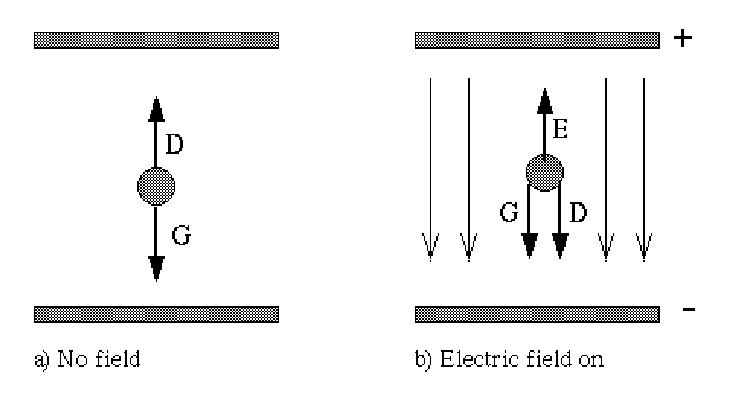
\epsfig{file=Introduction/oil_droplet.eps, height=5cm}
  \caption{
    Forces on an oil-droplet in: \newline
    \hspace*{1.5cm}
           a) Free fall          \newline
    \hspace*{1.5cm}
	   b) Electric field     \newline
    (G=Gravitation, D=Drag, E=Electric force)
  }
  \label{oil_droplet}
\end{center}
\end{figure}

His results were systematically low by about 4\% due to inaccurate
knowledge of the coefficient of viscosity. \newline
The electron charge is -e,
where $e = 1.602 \cdot 10^{-19}C$. All free particles are observed to
have values of electric charge equal to an integer times the
fundamental charge e:

\begin{equation*}
  q=n e
\end{equation*}

where the integer $n=\dots,-1,0,1,\dots$ is the electric charge
\emph{quantum number}.

\subsection*{The Nucleus}

In 1912, Ernest Rutherford and his associates discovered that the
positive charge of the atom is concentrated in a \emph{nucleus}. The
charge of the $\alpha$ particle, discovered by Becquerel, was
determined to be $2e$, and the mass of the $\alpha$ particle was
determined to be about four times the mass of the hydrogen
atom. \newline
A new particle with zero electric charge was discovered by bombarding
beryllium atoms with $\alpha$ particles. James Chadwick showed that
the new particle, the \emph{neutron}, had mass nearly equal to that of
the \emph{proton}.

\subsection*{The Bohr Model of the Atom}

In 1913, Niels Bohr made the first qunatitatively successful model of
the atom. Inspired by the work of Rutherford, Bohr made a planetary
model of the atom; with electrons moving in circular orbits about the
nucleus. This model may seem quite simple in retrospect, but for the
time it was a great advancement of science. In addition to the
classical circular orbits, the second part of Bohr's atomic model
contains a bold hypothesis of new physics. The new physics recognizes
that \emph{angular momentum} is \emph{quantized}; it can take only
certain values:

\begin{equation*}
  L = mvr = n \hbar
\end{equation*}

where $n$ is a positive integer. Solving the energy equations result
in orbits of radius:

\begin{equation*}
  r_n = \frac{n^2\hbar^2}{mke^2}
\end{equation*}

where the \emph{Bohr radius}

\begin{equation*}
  a_0 \equiv r_1 = \frac{\hbar^2}{mke^2} \approx 0.053 nm
\end{equation*}

is in the correct order of magnitude for the size of the atom!

{\bf Planc }





%               The Two First Excited states of Helium
\subsection{The Two First Excited states of Helium}

We will not make any calculations regarding exited states in this
thesis, but it is a really important issue in quantum mechanics. The
ground state energy does not tell much about the 
chemical properties of the atom on its own. Therefore good
approximations of the exited states are needed. Also, when discussing
different numerical approaches for solving the many body-problem,
including linear combinations of exited states may greatly improve
some original approximation to the ground state. Furthermore,
understanding how we include exited states is important for fully
understanding the application of the Slater determinant.
\newline
%
\newline
The state of helium with the $1s$ and the $2s$ orbitals occupied
with one electron each. 








The construction of the
periodic table in the second half of the $19^{\mathrm{th}}$ century
was based on the chemical properties of the different atoms. These
properties were not understood until the development of quantum
mechanics. The electrons are filled from the energetically lowest
orbitals. In the $s$ orbitals only two electrons of different
spins are allowed. Disregarding electron repulsion this would imply
that twice the energy is needed in removing an electron from ground
state helium than from the ground state hydrogen. This due to the 
double electric charge of the helium nucleus. The ionization energy of
hydrogen is $13.60 eV$ and the ionization energy of helium is $24.58
eV$ (ref. \cite{atkins2003}). The electron repulsion thus reduce the
ionization energy by almost $10\%$.
\newline
%
\newline
The early development of quantum theory may be summarized through the
four postulates of quantum mechanics.


%*************** The Postulates of Quantum Mechanics **************
%*
%*
\section{The Postulates of Quantum Mechanics}

A common formulation of quantum mechanics is by means of linear
algebra. In this formulation every state is represented as a (usually
infinite dimensional) complex vector, and an operator is represented
as a complex, linear and hermitian matrix. 
The postulates of quantum mechanics fall naturally into two sets: the
first three, which tell us how the system is depicted at a given time,
and the fourth, which specifies how this picture changes with time. 
\newline

%*                     The First Postulate                              *
%\subsection{The First Postulate}

{\bf \large Postulate 1}
\emph{
The state of a quantum mechanical particle is described by a vector
$\Psi$ in a Hilbert space ${\cal H}$. All the possible states of the
particle are ${\cal H}$ except the zero vector.
\newline
}

The first postulate states that a particle is described as a vector in
the Hilbert space. So a particle with finite degrees of
freedom $\mathbf{x}$ and $\mathbf{p}$ in classical
mechanics, now has infinite degrees of freedom. 
\newline

%*                     The Second Postulate                              *
%\subsection{The Second Postulate}

{\bf \large Postulate 2}
\emph{
Every observable are represented by an Hermitian linear operator in
${\cal H}$. For every classical dynamical variable
$\omega(\mathbf{x},\mathbf{p})$ there is a corresponding quantum
mechanical operator $\Omega$  obtained by operator substitution of the
fundamental position and momentum operators $\mathbf{X}$ and
$\mathbf{P}$, respectively: 
}
%
\begin{equation*}
  \Omega(\mathbf{X},\mathbf{P}) = \omega(\mathbf{x} \to
  \mathbf{X},\mathbf{p} \to \mathbf{P})
\end{equation*}
%
\emph{
The components of $\mathbf{X}$ and $\mathbf{P}$ are operators defined
through the fundamental commutation relation
}

\begin{equation*}
  \left[ X_i, P_j \right] = i \hbar \delta_{ij}
\end{equation*}

The second postulate tell us how to to move from the classical to the
quantum mechanical picture. The observables (or measurable quantities)
are defined through an operator. This operator may be obtained by
simple substitution of the position and the momentum of the
corresponding classical observable.
\newline

%*                     The Third Postulate                              *
%\subsection{The Third Postulate}

{\bf \large Postulate 3}
\emph{
The only possible values obtainable in an (ideal) measurement of an
observable $\Omega$ are its eigenvalues $\omega_n$. Each have a
probability
}
%
\begin{equation*}
  P(\omega_n) = \frac{\int \Psi^* \Phi_n }{\int \Psi^* \Psi }
\end{equation*}
%
\emph{
with $\Phi_n$ the eigenfunction corresponding to the eigenvalue
$\omega_n$. Immediately after a measurement the state collapses into
$\Phi_n$.
}
\newline

The third postulate tells what may be extracted from the quantum
mechanical picture by means of measurements. Note that the eigenvalues
may either have a continuous spectrum or be \emph{quantized}.
\newline


%*                     The Fourth Postulate                              *
%\subsection{The Fourth Postulate}

{\bf \large Postulate 4}
\emph{
The time development of the quantum state $\Psi$ is given by the time
dependent Schr\"odinger equation,
}

\begin{equation*}
  \hat{H} \Psi(\mathbf{x},t) = i\hbar \frac{\delta}{\delta
  t}\Psi(\mathbf{x},t) 
\end{equation*}

The fourth and final postulate defines the Schr\"odinger
equation. This equation describes how the quantum mechanical state
evolve in time.
\newline






\chapter{Electronic Systems}
\label{ch:electronic_systems}
This chapter will be devoted to the theoretical treatment of some of the systems our program will be able to handle. The aim is to present single-particle wave functions which are good starting points 
for our many-body studies. Examples of such widely used 
single-particle wave functions are the the solutions 
to the harmonic oscillator problem or the solutions to hydrogen-like problems.

These single-particle wave functions are in turn used in constructing the so-called Slater determinant,
which together with a correlation part, is a key part of our ansatz for the trial wave functions
used in the Monte Carlo algorithm. 
\section{The Harmonic Oscillator}
The harmonic oscillator describes systems where the force 
on a particle is proportional to the distance from an equilibrium position. 
The most famous example is of course that of a mass coupled to a spring which abides to Hooke's law. However, many other systems such as molecules, motions of an atom in a lattice and phonons can be described as either one or a collection of harmonic oscillators. In this section we will first review the one particle system in one dimension and then generalize to $d$ dimensions. 
Since we confine ourselves to electronic systems, our particles are electrons. However, our formalism
can easily be extended to other particle species, such as neutrons and protons.

%Finally we will discuss the problems of interacting particles for which an analytical solution only exist in the two-particle case for specific values of $\omega$.
\subsection{One Dimension}
 The one-particle harmonic oscillator Hamiltonian in one dimension is 
%
\bea
H &=& \frac{1}{2m_e} {p}^2 + \frac 1 2 m_e\omegasq x^2,\\
     &=& - \frac{\hbar^2}{2m_e}\dd x + \frac 1 2 m_e\omegasq x^2,
\eea
%
where $\omega$ is the oscillator frequency and $m_e$ is the electron mass.  The time independent Schr\"odinger equation $H \phi = E\phi$ becomes
%
\be
- \frac{\hbar^2}{2m_e}\ddf \phi x + \frac 1 2 m_e\omegasq x^2 \phi = E\phi.
\ee
%
Before we solve this it is convenient to introduce  dimensionless variables
%
\bea
\underline x &=& \frac{x}{\sqrt{\hbar/m_e\omega}},\\
\eps &=& \frac{2E}{\hbar \omega}.
\eea
% 
Dropping the underline in $\underline x$ and using the prime notation to indicate derivation we get
%
\be
\phi''  + (\eps-x^2)\phi = 0. 
\label{eq:schrodinger}
\ee
%
This is a second-order linear homogeneous differential equation. 
To solve it we first look at the behaviour when $x\rightarrow \infty$. In this case we can neglect the $\eps$ term and get
%
\be
\phi'' = x^2\phi, \quad x\rightarrow \infty.
\label{eq:schrodingeratinf}
\ee
%
We need a function that when derivated gives back the original function times $x$. The two functions $\phi(x) = e^{\pm \frac {x^2}{2}}$ do exactly this.  Inserting them into eq.~(\ref{eq:schrodingeratinf})
%
\be
\phi'' = (x^2+1)\phi \approx x^2\phi, \quad x\rightarrow \infty.
\ee
%
Since a wave function must be normalizable, only the function $\phi(x) = e^{-\frac {x^2}{2}}$ belongs to the physical Hilbert space. The solution is therefore of the type $\phi(x) = f(x)e^{-\frac {x^2}{2}}$ for some unknown function $f$. Inserting this into eq.~(\ref{eq:schrodinger}) we end up with 
%
\be
f''-2xf'+(\eps-1)f=0.
\label{eq:power}
\ee
%
This type of equation is solved by the power series method where we assume that $f(x)$ is represented
by a polynomial in $x$, namely 
$f(x) = \Sum_{k=0}^\infty a_k x^k$. The derivatives are
%
\bea
f'  &=& \Sum_{k=0}^\infty k a_k x^{k-1},\\
f'' &=& \Sum_{k=0}^\infty k(k-1) a_k x^{k-2},
\eea
%
which inserted into eq.~(\ref{eq:power}) give
%
\be
\Sum_{k=0}^\infty  k(k-1) a_k x^{k-2} + 2k a_k x^{k} + (\eps-1)a_k x^k = 0.
\ee
%
To obtain a recursion relation we notice that the two first terms in $f''$ will be zero because of the $k(k-1)$ factor. Changing variables $k$ with $k+2$ we get
%
\be
f'' = \Sum_{k=0}^\infty k(k-1) a_k x^{k-2} = \Sum_{k=0}^\infty (k+2)(k+1) a_{k+2} x^{k}, 
\ee
%
which results in
%
\be
\Sum_{k=0}^\infty  \left[ (k+2)(k+1) a_{k+2} -(2k + 1 -\eps)a_k\right] x^k = 0,
\ee
%
which is only fulfilled for all $x$ when the terms inside the brackets vanish for all $k$, viz.,
%
\be
a_{k+2} = \frac{2k + 1 -\eps}{(k+2)(k+1)}a_k, \quad k=0,1,2,\ldots
\ee
%
and the first two coefficients, $a_0$ and $a_1$, can be chosen freely. The series will diverge for large $x$ if there are no restrictions on $\eps$. We show this by noting that for large $x$, the coefficients for large $k$ will be dominate the series
%
\be
\frac{a_{k+2}}{a_k} \simeq \frac 2 k.
\ee
%
Comparing this result with the recursion relation for the power series expansion of $e^{x^2}$
%
\bea
e^{x^2} &=& \Sum_{k=0,2,4,\ldots} b_k x^k,\\
b_k &=& \frac{1}{(\frac 1 2 k)!}
\eea
%
which gives the coefficient ratio
%
\be
\frac{b_{k+2}}{b_k} = \frac{(\frac 1 2 k)!}{(\frac 1 2 (k+2))!}=\frac 1 {\frac 1 2 k +1} \simeq \frac 2 k,
\ee
%
we see that the divergence is a fact. The only way to avoid this is by terminating the series so that $f(x)$ becomes a  polynomial with a finite number of powers in $x$. 
This is possible by restricting
%
\be
\eps = \eps_n = 2n + 1, \quad n=0,1,2,\ldots,
\label{eq:quantized_energy}
\ee
%
and choosing $a_1=0$ for even $n$ or $a_0=0$ for odd $n$. We have in other words just showed that the energy for the harmonic oscillator is quantized. To find the polynomials $f_n(x)$ we insert eq.~(\ref{eq:quantized_energy}) into eq.~(\ref{eq:power}) and get
%
\be
f_n'' - 2xf_n' + 2nf_n, \quad n=0,1,2,\ldots
\ee
%
It can be shown that the solution to these equations are the Hermite polynomials $H_n(x)$ which are defined as
%
\be
H_n(x) = e^{x^2}\left( -\sd x \right)^n e^{-x^2}.
\ee
%
Using recursion relations
\bea
H_{n+1} &=& 2xH_n -2nH_{n-1},\\
H_n' &=& 2nH_{n-1}.
\eea
the first five terms are 
\bea
H_0 &=& 1, \\
H_1 &=& 2x, \\
H_2 &=& 4x^2 -2, \\
H_3 &=& 8x^3 - 12x, \\
H_4 &=& 16x^4 - 48x^2 +12.
\eea
The Hermite polynomials have alsotwo other important properties
%
\bea
\int_{-\infty}^{\infty} H_n(x)H_m(x) e^{-x^2} &=& 0, \quad n \neq m\\
\int_{-\infty}^{\infty} H_n^2(x) e^{-x^2} &=& 2^n n! \int_{-\infty}^{\infty} e^{-x^2} = \sqrt \pi \,2^n n!, 
\eea
%
which tells us that the wave functions are orthogonal and normalized. 
Switching back to normal coordinates (that it is inserting the correct dimensions) we get 
%
\bea
\phi_n(x) &=& \left( \frac{m_e\omega}{\pi\hbar} \right)^{\frac 1 4} \frac{1}{\sqrt{2^n n!}}e^{-m_e\omega x^2/2\hbar} \, 
H_n(x\sqrt{m_e\omega /\hbar})\\
E_n &=& (n+\frac 1 2)\hbar \omega
\eea
%
We see that the ground state has a non zero energy whereas the classical counterpart has not. %which has implications
\subsection{Harmonic oscillator in $d$ dimensions}
It is fortunately very easy to solve the general $d$ dimensional case once the one dimensional case is obtained. The Hamiltonian is
%
\be
H = \Sum_{r=1}^d H_r = \Sum_{r=1}^d \left(-\frac{\hbar^2}{2m_e}\dd{x_r} + \frac 1 2 m \omegasq_r x_r^2\right), 
\ee
%
which is a sum over $d$ independent parts. This suggests a wave function on the form
%
\be
\phi_N(x_1,\ldots,x_d) = \Prod_{r=1}^d \phi_{n_r}(x_r), \quad N=n_1,\ldots,n_d.
\ee
%
If we identify $n_1=n_x$, $n_2=n_y$, $x_1=x$, $x_2=y$ and so forth, the Schr\"odinger equation 
can be written as 
\be
\phi_N^{-1}H\phi_N=E_N,
\ee
resulting in
%
\be
\Sum_{r=1}^d \left( -\frac{\hbar^2}{2m_e} \frac{\phi_{n_r}''}{\phi_{n_r}} + \frac 1 2 m \omegasq_r x_r^2 \right) = E_N.
\ee
%
This can only be fulfilled if each term in the sum is a constant that adds up to $E_N$
%
\bea
-\frac{\hbar^2}{2m_e} \frac{\phi_{n_r}''}{\phi_{n_r}} + \frac 1 2 m \omegasq_r x_r^2 &=& E_r, \quad r=1,2,\ldots,d\\
\Sum_{r=1}^d E_r &=& E_N.
\eea
%
We thus end up with $d$ one dimensional equations that we already know the solution to 
%
\bea
\phi_N(x_1,\ldots,x_d) &=& \Prod_{r=1}^d 
\left( \frac{m_e\omega_r}{\pi\hbar} \right)^{\frac 1 4} \frac{1}{\sqrt{2^{n_r} 
n_r!}}e^{-m_e\omega_r x_r^2/2\hbar}\nonumber\\ && \times H_{n_r}(x_r\sqrt{m_e\omega_r /\hbar})\\
E_N &=& \Sum_{r=1}^d (n_r+\frac 1 2)\hbar \omega_r.
\eea
%
In the special case of an isotropic oscillator potential $\omega_r=\omega$ the energy is 
%
\bea
E_N &=&  (N +\frac d 2)\hbar \omega\\
N &=& \Sum_{r=1}^d n_r. 
\eea
%
Thus all the excited states are degenerate because different combinations of $n_r$ will yield the same $N$. To calculate the spatial degeneracy $g_r(N)$ we note that $n_x = 0,1,\ldots,N$ which are $N+1$ different values. In the two dimensional case $n_y=N-n_x$ so the degeneracy is just $g_2(N)=N+1$. If we include the spin degrees of freedom, the total degeneracy $G_2(N)$ becomes
%
\be
G_2(N)=2(N+1).
\ee
%
As we add more and more electrons to the system (obeying the Pauli principle), 
they will be in the state which gives the lowest total energy for the system. If we measure how much energy is required to add or remove an electron it will depend on how many electrons $N_e$ currently 
are in the system. The energy needed will have spikes at certain magic numbers $N_e = S_r(N)$ which corresponds to the case when all degenerate statesup to a given single-particle level 
are occupied. This is given by the formula
\be
S_r(N) = \Sum_{i=1}^N G_r(i).
\ee
The resulting shell structure for the two dimensional case is displayed in table~(\ref{table:2DHOShellStructure})
\begin{table}[h!]
  \centering
  \[
  \begin{array}{r|r|r|r|r}
    N&n_x&n_y&G_2(N)&S_2(N)\\
    \hline
    0&0&0&2&2\\
    1&1/0&0/1&4&6\\
    2&2/1/0&0/1/2&6&12\\
    3&3/2/1/0&0/1/2/3&8&20\\
  \end{array}
\]
\caption{Shell structure for two dimensional harmonic oscillator including combinations of $n_x$ and $n_y$}
\label{table:2DHOShellStructure}
\end{table}
The spatial degeneracy in three dimensions case is found by noting that $n_y = 0,1,\ldots,N-n_x$ which are $N-n_x+1$ different values for each $n_x$. To get the total number of different values we have to sum over all $n_x$
%
\bea
g_3(N) &=& \Sum_{n_x=0}^N (N+1-n_x),\\
       &=& (N+1)^2 - \frac{N(N+1)}{2},\\
       &=& (N+1)(N+1-\frac N 2),\\
       &=& \frac 1 2 (N+1)(N+2),
\eea
%
which gives a total degeneracy
\be
G_3(N)= (N+1)(N+2).
\ee
The shell structure is showed in table~\ref{table:3DHOShellStructure}
\begin{table}[h!]
  \centering
  \[
  \begin{array}{r|r|r}
    N&G_3(N)&S_3(N)\\
    \hline
    0&2&2\\
    1&6&8\\
    2&10&20\\
    3&20&40\\
  \end{array}
\]
\caption{Shell structure for three dimensional harmonic oscillator}
  \label{table:3DHOShellStructure}
\end{table}
The spatial degeneracy is related to the symmetry in the potential 
%
\be
V(x_1,\ldots,x_d) = \Sum_{r=1}^d \frac 1 2 m_e\omega x_r^2 = \frac 1 2 m_e\omega r^2 = V(r),
\ee
%
because when the harmonic oscillator is isotropic, each dimension contributes the same amount of energy.

\section{Quantum Dots}
Quantum dots are a man made system of trapped electrons that share some properties with atoms, 
hence the popular name ``designer atoms''. Their size ranges between 100 nm to 1 $\mu$m which 
is much larger than a regular atom. Atoms have typically spatial extensions that are of the size of 
0.05-0.4 nm. The quantum dot is created in a semiconductor, typically gallium arsenide (GaAs), 
and confined either by a physical barier, such as an insulator like aluminum gallium arsenide (AlGaAs), 
or an electric field. The confinement gives rise to a bowl shaped potential that can be 
approximated by the harmonic oscillator potential. 
One application of the quantum dot is as the qubit in a quantum computer by manipulating the electron states. Another is in biology for fluorescent labelling of both normal and cancer cells .  
\newline

We will first consider the two dimensional quantum dot and then extend our system 
to three dimensions. The purpose is to show that as long as the two-particle repulsive Coullomb interaction does not depend on spin, that the magnetic field will only result in an 
effective harmonic oscillator potential and a constant shift in the energy spectrum. 

\subsection{Two dimensions}
We first consider the case with no electron-electron repulsion.
This means that the Hamiltonian contains only onebody operators.
The Hamiltonian is derived in \ref{app:qdhamiltonian} and the result is 
%
\bea
\hat H &=& \frac{1}{2\meff} \left(\f p - \frac e c \f A\right)^2 + \frac 1 2 \meff\omegazsq (x^2+y^2) + e\phi - \f \mu_S \cdot \f B,   
\eea
%
where $\f A$ and $\phi$ is the vector and scalar potentials associated with the external electromagnetic field. The last term in the Hamiltonian is the coupling of the electron spin magnetic moment $\f \mu_S$, to the magnetic field and $\meff$ is the effective electron mass. We will consider the special case of a constant and uniform magnetic field along the z-axis, $\f B=(0,0,B)$, and no electric field. The vector and scalar potentials are related to the electromagnetic field by the equations
%
\bea
\f E &=& -\frac 1 c \pdf {\f A} t - \nabla \phi\\
\f B &=& \nabla \times A. 
\eea
%
It is easy to see that we can only obtain a constant magnetic field if also $\f A$ is constant in time. The scalar potential is now given by
%
\be
\nabla \phi = 0,
\ee
%
which has  only the solution $\phi = k$ where $k$ is a constant. We will however set $k=0$ for the rest of this derivation. Before choosing $\f A$, we expand the first term in the Hamiltonian
\be
(\f p - \frac e c \f A)^2 = p^2 - \frac e c (\f p \cdot \f A + \f A \cdot \f p) + \frac {e^2}{c^2}A^2,
\label{eq:pminusAsq} 
\ee
and in general 
\be
\f A(x,y,z) = (A_x(x,y,z), A_y(x,y,z), A_z(x,y,z) ).
\ee
This means that $\f A$ and $\f p$ will not commute unless we demand 
\be
\f A(x,y,z) = (A_x(y,z), A_y(x,z), A_z(x,y) ).
\ee
In this case we have $\nabla \cdot A = 0$, which means that we are working in the coulomb gauge. One 
possibility for the vector potential is $\f A = \frac B 2 (-y, x, 0)$ and by inserting this into eq.~(\ref{eq:pminusAsq} ) we get
\be
(\f p - \frac e c \f A)^2 = p^2 - \frac{eB}c (xp_y - yp_x) + \frac{e^2B^2}{4c^2}(x^2 + y^2)
\ee
We note that $xp_y - yp_x = L_z$, where $L_z$ is the angular momentum operator in the z direction. Inserting this into the Hamiltonian we get
\bea
H &=&  \frac 1 {2\meff} \left[p^2 - \frac{eB}{c} L_z + \frac{e^2B^2}{4c^2}(x^2 + y^2) \right] + \nonumber \\
&&     \frac 1 2 \meff\omegazsq (x^2+y^2)  + \frac{e g_s^* B}{2\meff c} S_z
\eea
where $g_s^*$ is the effective spin-gyromagnetic factor. It is easy to check that both $L_z$ and $S_z$ commute with the Hamiltonian. This means that the solution of the 
stationary Schr\"odinger equation will be an eigenfunction of $L_z$ and $S_z$. The $L_z$ operator has a simple representation in polar coordinates 
\be
L_z = -i\hbar \left(x \pd y - y \pd x \right) = -i\hbar \pd \varphi
\ee
with eigenfunction $e^{im\varphi}$ and eigenvalue $\hbar m$. Because the angles $\varphi$ and $\varphi + 2\pi$ are required to give the same eigenfunction, $m$ is restricted to the values $m=0,\pm 1, \pm 2,\ldots$. The spin operator $S_z$ is represented by the matrix
\be
S_z = \frac \hbar 2 \begin{pmatrix} 1&0\\0&-1 \end{pmatrix}
\ee
 and its eigenfunction is the two component spinor
\be
 \f \chi = \begin{pmatrix} c_1\\c_2 \end{pmatrix}
\ee
where $|c_1|^2$ and $|c_2|^2$ are the probabilities for a state with spin up and spin down, 
respectively. The eigenvalues are $\pm \hbar/ 2$ and tell us that the spin up state has a higher energy than the spin down state. This is the Pauli equation modified with the addition of a harmonic oscillator potential and we know that the spatial part of the wave function is equal for both spinor components. More formally we write the total wave function as
\be
\f \phi = \phi \f \chi,
\ee
and split the Hamiltonian in a spatial part and a spin part
\be
H = H_\Omega + H_s, 
\ee
where
\be
H_s = \frac{e g_s^* B}{2\meff c} S_z.
\ee
The stationary Schr\"odinger equation becomes
\be
\f \chi H_\Omega \phi + \phi H_s \f \chi = E \phi \f \chi 
\ee
which separates into the following system of coupled equations
\bea
\label{eq:spatial}
 H_\Omega \phi &=& E_\Omega \phi,\\
 H_s \f \chi &=& E_s \f \chi,
\eea
where $E_\Omega + E_s = E$. Solving the last one is very easy since $H_s$ is just a constant times $S_z$
\be
E_s = \frac{e \hbar g_s^* B}{2\meff c}s, 
\ee
where $s=1/2$ for spin up and $s=-1/2$ for spin down. 
\newline
\newline
We now move on to solving eq.~(\ref{eq:spatial}). Due to the spatial symmetry in the Hamiltonian we switch to polar coordinates and define
\bea
\omega_B &=& \frac{eB}{2\meff c}\\
\omegasq &=& \omegazsq + \omega_B^2.
\eea
The spatial part of the Hamiltonian is now
\be
H_\Omega = H_{r\varphi} = -\frac{\hbar^2}{2\meff}\left(\pdd r + \frac 1 r \pd r + \frac 1  {r^2} \pdd \varphi \right) 
               + i\hbar\omega_B \pd \varphi  + \frac 1 2 \meff \omegasq r^2,
\ee
which is separable in $r$ and $\varphi$. This means that the spatial part of the wave function is also separable
\be
\phi_m(r,\varphi) =R(r)e^{im\varphi}.
\ee
Feeding this into the stationary Schr\"odinger equation results in the following linear ODE in $R(r)$
\be
 - \frac{\hbar^2}{2\meff}\left(\pdd r + \frac 1 r \pd r - \frac{m^2}{r^2} \right)R(r)
 + \frac 1 2 \meff \omegasq r^2 R(r) = \eps_m R(r),
\ee
where $\eps_m = E_\Omega-\hbar m \omega_B$. This equation is solved by using the same technique as for the one-dimensional harmonic oscillator. We omit therefore the derivation. The normalized solution is
\bea
\label{eq:radial2d}
R_{nm}(r) &=& \sqrt{\frac{2n!}{(n+|m|)!}} \beta^{(|m|+1)/2} r^{|m|}e^{-\beta r^2/2} L_n^{|m|}(\beta r^2),\\
E_\Omega = E_{nm}    &=& (2n + |m| + 1)\hbar\omega + \hbar m\omega_B ,
\eea
where $n=0,1,2,\ldots,$ and
\be
\beta = \frac{\meff \omega} \hbar,
\ee
and $L_n^{|m|}(\beta r^2)$ is the associated Laguerre polynomial which in the Rodriguez representation is defined as
\be
L_n^{m}(r) = \frac 1 {n!} e^r r^{-m} \pdn r \left(e^{-r} r^{n + m} \right). 
\ee
The first three polynomials are
\bea
L_0^{m}(r) &=& 1,\\
L_1^{m}(r) &=& -r + m + 1,\\
L_2^{m}(r) &=& \frac 1 2 r^2 -(m+2)r + \frac 1 2 (m+2)(m+1). 
\eea
In order to get $\phi_{nm}(r,\varphi)$ we just have to multiply eq.~(\ref{eq:radial2d}) with the normalized angular part. The result is
\be
\phi_{nm}(r,\varphi) = \sqrt{\frac{n!}{\pi(n+|m|)!}} \beta^{(|m|+1)/2} r^{|m|}e^{-\beta r^2/2} 
                       L_n^{|m|}(\beta r^2) e^{im\varphi}. 
\ee
The total energy of the system is
\be
E = E_{nms} = E_{nm} + E_s = (2n + |m| + 1)\hbar\omega + m\hbar\omega_B  + g_s\hbar\omega_B s,
\ee
and to analyze the effect of the magnetic field we compare this energy to 
\be
E_{B=0} = E_{nm} =(2n + |m| + 1)\hbar\omega_0.  
\ee
In this case we regain the energy spectrum of a two-dimensional harmonic oscillator 
as we should, but with different quantum numbers reflecting the change to polar coordinates. 
Clearly $N=2n+|m|$, and the shell structure is shown in table~(\ref{table:2DHO}). We see that the presence of the magnetic field makes the energy depend on the sign of $m$ and $s$. The previous degenerate states will now separate more and more as the magnetic field increases. When there are no degeneracies left, the concept of shell structure may at first seem problematic. However for small magnetic fields the ionization energy will still have peaks at the same magic numbers as for the degenerate case. Of course, for strong magnetic fields this picture breaks down. We should also mention that for some special magnetic field strengths some of the non degenerate energy levels will overlap and we can have so called accidental degeneracies. One example is when $\omega_0/\omega_B = \sqrt{(1+g_s^*)^2 - 1}$ which would make $E_{00\frac 1 2}=E_{0 -1 -\frac 1 2}$. 
\begin{table}[h!b]
  \centering
      \begin{tabular}[]{r|r|r}
      $N$&$n$&$m$\\
      \hline
      0&0&0\\
      1&0&$\pm 1$\\
      2&$0/2$&$\pm 2/0$\\
      3&$0/1$&$\pm 3/\pm 1$\\
    \end{tabular}
    \caption{Shell structure for two dimensional harmonic oscillator with polar coordinate quantum numbers}
    \label{table:2DHO}
\end{table}
%
\newline
\newline
We want to briefly mention the relationship between the wave functions of the harmonic oscillator in polar and Cartesian coordinates by comparing the wavefunctions for $N=1$. I will use atomic units and omit
 the normalization factors in order to simplify the relations. In Cartesian coordinates the wave functions  are given by
\bea
\phi_{10} &=& xe^{\frac \omega 2 (x^2+y^2)},\\
\phi_{01} &=& ye^{\frac \omega 2 (x^2+y^2)},
\eea
while in polar coordinates they are
\bea
\phi_{01} &=& re^{\frac \omega 2 r^2}e^{(i\varphi)},\\
\phi_{0 -1} &=& re^{\frac \omega 2 r^2}e^{(-i\varphi)}.
\eea
By using the following relations
\bea
e^{(\pm i\varphi)} &=& \cos \varphi \pm i\sin\varphi\\
x &=& r\cos\varphi\\
y &=& r\sin\varphi
\eea
we can write the last two wavefunctions as
\be
\phi_{0\pm1} = e^{\frac \omega 2 (x^2+y^2)} \left(x\pm iy\right).
\ee
They are thus related to each other by the normalized linear combination
\be
\phi_{0\pm1} = \frac 1 {\sqrt2} \left(\phi_{10} \pm i\phi_{01}\right).
\ee
It also tells us that the two eigenfunctions of $L_z$ are $x\pm i y$, with 
eigenvalues $\pm \hbar$. %To our knowledge there is no general formula for the transformation of the wavefunctions in different coordinate systems. 
 %The Hermite polynomial relates to the Laguerre polynomial by the equations
%\bea
%H_{2n}(x) &=& (-4)^n n! L_n^{ -\frac 1 2}(x^2),\\
%H_{2n+1}(x) &=& 2(-4)^n n! x L_n^{\frac 1 2}(x^2).
%\eea

\subsection{Three dimensions}
The only change in the Hamiltonian is the inclusion of the $z$-direction. Thus the spatial Hamiltonian reads
\be
H_\Omega =  \frac 1 {2\meff} \left[p^2 - \frac{eB}{c} L_z + \frac{e^2B^2}{4c^2}\left(x^2 + y^2\right) \right] +
    \frac 1 2 \meff\omegazsq \left(x^2+y^2\right) + \frac 1 2 \meff\omega_z^2 z^2
\ee
where $p^2$ now includes $p_z^2$. The $L_z$ operator commutes with $H_\Omega$, however, an analytical solution is only attainable when $\omega_z = \omega$ since the magnetic field 
only shifts the part of the oscillator potential that is perpendicular to the magnetic field. 
Using this and changing to polar coordinates we get
\bea
H_{r\theta\varphi} &=&  -\frac{\hbar^2}{2\meff}\left[\pdd r + \frac 2 r \pd r + \frac 1  {r^2}
\left( \frac 1 {\sin^2\theta} \pdd \varphi + \cot\theta\pd \theta + \pdd \theta\right) \right]\nonumber\\
&&               + i\hbar\omega_B \pd \varphi  + \frac 1 2 \meff \omegasq r^2.
\eea
The part inside the parenthesis is equal to the operator $-\frac{1}{\hbar^2}L^2$ which also commutes with $H_{r\theta\varphi}$. Its eigenfunctions are the spherical harmonics $Y_{lm}$ which in normalized form are
\be
\label{eq:SphericalHarmonics}
Y_{lm}(\theta,\varphi) = \delta_m\left[\frac{(2l+1)(l-|m|)!}{4\pi(l+|m|)!} \right]^{\frac 1 2}
P_l^{|m|}(\cos\theta) e^{im\varphi},
\ee
with the requirement $l=0,1,2,\ldots,$ and $m=0,\pm 1, \pm 2, \ldots,\pm l$ and where
\be
\delta_m = \begin{cases}
(-1)^m& m \geq 0,\\
1&      m \leq 0.
\end{cases}
\ee
The associated Legendre polynomials $P_l^m$ are in the Rodriguez representation defined as
\be
P_l^m(x) = \frac{(-1)^m}{2^l l!}(1-x^2)^{\frac m 2}\left( \sd x \right)^{l+m}(x^2-1)^l,\quad |m| \leq l,
\ee
and the six lowest-order associated Legendre polynomials 
are shown in table~(\ref{table:LegendrePolynomials}). The eigenvalues of $L^2$ are $\hbar^2 l(l+1)$. 
\begin{table}[h!b]
  \centering
    \begin{tabular}{r|r|r}
      $|m|$&$l$&$P_l^m(x)$\\
      \hline
      0&0&1\\
      0&1&$x$\\
      0&2&$\frac 1 2(3x^2 - 1$\\
      1&1&1$-\sqrt{1-x^2}$\\
      1&2&$-3x\sqrt{1-x^2}$\\
      2&2&$3(1-x^2)$\\
    \end{tabular}
    \caption{Lowest order associated Legendre polynomials}
    \label{table:LegendrePolynomials}
\end{table}
%
The Hamiltonian is once again separable. An ansatz for the wave function is then
\be
\phi_{lm}(r,\theta,\varphi) = R(r)Y_{lm}(\theta,\varphi). 
\ee
Inserting this into the stationary Schr\"odinger equation we end up with the differential equation
\be
- \frac{\hbar^2}{2\meff}\left(\pdd r + \frac 2 r \pd r - \frac{l(l+1)}{r^2} \right)R(r)
 + \frac 1 2 \meff \omegasq r^2 R(r) = \eps_m R(r),
\ee
which is quite similar to the two-dimensional one. The solution is
\bea
R_{nl}(r) &=& \left[\frac{2n!}{(n+l+1/2)!}\right]^{1/2} \beta^{(l+3/2)} r^l e^{-\beta r^2/2} L_n^{l+1/2}(\beta r^2),\\
E_\Omega = E_{nlm} &=& (2n+l+\frac 3 2)\hbar\omega + \hbar m\omega_B
\eea
with n=0,1,2,\ldots. As expected, there are no degenerate energy levels 
and if we set $B=0$ we regain the energy spectrum of the harmonic oscillator by identifying $N=2n+l$. 
\subsection{Two-particle system}
We will now present how the problem of a two electron quantum dot can be solved analytically for certain values of $\omega$. These results are 
taken from the article \cite{MTautQDotAnalSol} and form an  important basis for checking our 
numerical solution method and also to gain some physical insight on the role of  
correlations. The spatial Hamiltonian in two dimensions is
\be
H_{r_\varphi} = \Sum_{i=1}^2 \left[\frac 1 {2\meff}\left(\f p_i - \frac e c \f A_i \right)^2 + \frac 1 2 \meff\omegazsq r_i^2 \right] + \frac{e^2}{4\pi\eps_0 |\f r_2 - \f r_1|}.
\ee
By introducing the center-of-mass and relative coordinates we can split the Hamiltonian in two parts, one which depends on the relative coordinates only and one which depends on the center-of-mass coordinates. 
We can the use the separation of variables technique when solving the stationary Schr\"odinger equation. The coordinate transformation is given by
\bea
\f r &=& \f r_2 - \f r_1,\\
\f R &=& \frac 1 2 (\f r_1 + \f r_2),
\eea
where $\f R$ and $\f r$ are the center-of-mass term and the relative term, respectively. The momenta will also be transformed according to
\bea
\f p &=& \frac 1 2(\f p_2 - \f p_1), \\
\f P &=&  \f p_1 + \f p_2.
\eea
When $\f B$ is a constant, Maxwell's equations implies that $\f A$ must be linear
\bea
\f A(r) &=& \f A(r_2) - \f A(r_1),\\
\f A(R) &=& \frac 1 2 ( \f A(r_1) + \f A(r_2) ).
\eea
The following relations will come in handy when transforming the Hamiltonian
\bea
p_1^2 + p_2^2 &=& \frac 1 2 (P^2 + 4p^2),\\
r_1^2 + r_2^2 &=& \frac 1 2 (4R^2 + r^2),\\
|\f r_2 - \f r_1| &=& r\\
\f p_1 \cdot \f A(r_1) + \f p_2 \cdot \f A(r_2) &=& \f p \cdot \f A(r) + \f P \cdot \f A(R)\\
A_{r_1}^2 + A_{r_2}^2 &=& \frac12 A(r)^2 + 2A(R)^2
\eea
The result is
\begin{equation}
\begin{split}
H_{r_\varphi}&= \frac1{2}\left\{\frac1{2\meff} 
\left[P^2 -4\frac ec \f P \cdot \f A(R) + 4 \frac{e^2}{c^2}A(R)^2\right] 
+  2 \meff\omegazsq R^2 \right\} \\
&\;\; + 2 \biggl\{ \frac1{2\meff}\left[p^2 - \frac ec \f p \cdot \f A(r) + \frac14 \frac{e^2}{c^2}A(r)^2\right]
+  \frac18 \meff\omegazsq r^2 \\ 
& \;\; \qquad + \frac{e^2}{8\pi\eps_0 r}\biggr\},
\end{split}
\end{equation}
and by introducing
\bea
\label{eq:omegaR}
\omega_R &=& 2\omega_0\\
\omega_r &=& \frac12 \omega_0\\
\label{eq:AR}
\f A_{R} &=& 2 \f A(R)\\
\label{eq:Ar}
\f A_{r} &=& \frac12 \f A(r)
\eea
we get
\bea
H_{r_\varphi} &=& \frac 1 2\left\{\frac1{2\meff} \left[P-\frac ec \f A_{R}\right]^2
+  \frac12 \meff\omega_R^2 R^2 \right\} + \nonumber \\
&& \, 2 \left\{ \frac1{2\meff} \left[p - \frac ec \f A_{r}\right]^2
+  \frac12 \meff\omega_r r^2 + \frac{e^2}{8\pi\eps_0 r}\right\},\\
&\equiv&\frac12 H_R + 2H_r.
\eea
The wavefunction can the be written in  the product form  as 
\be
\Psi(\f r,\f R) = \psi_r(\f r) \psi_R(\f R)
\ee
and when inserted into the Schr\"odinger $H\Psi = E\Psi$ we end up solving the system of equations
\bea
\label{eq:rel}
H_r \psi_r &=& E_r \psi_r\\
\label{eq:com}
H_R \psi_R &=& E_R \psi_R
\eea
 with total energy
\be
E = \frac12 E_R + 2E_r.
\ee
The solution to the center-of-mass problem, eq~(\ref{eq:com}) is the same as for the one particle case. The energy will be
\be
E_R = E_{NM} = 2(N + |M| + 1)\hbar \omega + 2\hbar M \omega_{B} 
\ee
where the extra factor of two in comes from eq.~(\ref{eq:AR}) and eq.~(\ref{eq:omegaR}).
\newline

We now move on to solve eq.~(\ref{eq:rel}) which is the relative part. The presence of the $1/r$ term makes it impossible to get a general closed-form solution. 
Such solutions only exist for particular values of $\omega$ that can be 
found by solving $a_n=0$ where $a_n$ is given by the the following recurrence relation
\bea
a_0&\neq&0\\
a_1&=&\frac 1 {a_0'(2|m|+1)} \sqrt{\frac {2 \hbar} {\meff\omega}}a_0\\
a_n &=& \frac{1}{n(n+2|m|)}\biggl\{\frac 1 {a_0'}\sqrt{\frac {2\hbar} {\meff\omega}}a_{n-1}\nonumber\\ 
&&+ \left[2\left(n+|m|-1\right) -\eps_{nm}\right]a_{n-2}\biggr\}, \quad n\geq2
\eea
where 
\be
a_0' = \frac{8\pi\eps_0\hbar^2}{2\meff e^2},
\ee
and
\be
\eps_{nm} = 2(|m|+n),  \quad n\geq2. 
\ee
The energy is given by
\be
E_r =E_{nm} = \frac 1 2(|m|+n)\hbar\omega + \frac12 m \hbar\omega_B. 
\ee
The procedure is to chose a value for $n$ and insert $\eps_{nm}$ into the expression for $a_n$ and then solve $a_n=0$ with respect to $\omega$. The ground state is given by $n=2$ and $m=0$ which gives $\omega=1$ and energy $E_r=\hbar$. The ground state of the center of mass part is given by $N=M=0$ which gives energy $E_R=2\hbar$. The total energy for the ground state of a two particle quantum dot is then $E=3\hbar$. The energy for the non-interacting case is just the one particle energy multiplied with two (the spin part cancels) and will for the ground state be equal to the center of mass energy. We see that the interaction energy is $1/3$ of the total energy.
\newline

In the three dimensional case it can be shown that we only have to make the substitution $|m|=l+1/2$ in the above expressions. The energy is
\bea
E_R = E_{NLM} = 2(2N + L + \frac32)\hbar\omega + 2\hbar M \omega_{B}\\
E_r = E_{nlm} = \frac 1 2(n+l+\frac12)\hbar\omega + \frac12 m \hbar\omega_B.  
\eea
The ground state energy is given by $n=2,l=m=0$ and $N=L=M=0$ for the relative and center of mass part, respectively. This gives $\omega=1/2$ and total energy $E=2\hbar$ from which the interaction part contributes $1/4$. We see that the interaction part is more important in the two dimensional case. This is expected since lower dimensionalities give less degrees of freedom. 

\section{Atomic systems}
We want to show that our program is capable of solving multi electron atoms by using the Slater determinant of hydrogen like wavefunctions. These wavefunctions are found by solving the stationary Schr\"odinger equation for one electron in an atom with $Z$ protons. This is a $Z+1$ body problem that is in general not analytically solvable. Howewer, we can exploit that the nucleus is much heavier than the electron by many orders of magnitude. The effect will be that the nucleus is almost at rest compared to the electron. We will therefore approximate the problem by treating the nucleus as having no kinetic energy. Though one should note that this approximation will only be accurate if the momenta of the nucleus and the electron is of the same order of magnitude. This is easily shown by comparing their kinetic energy $T$ given by
\bea
T_e &=& \frac {P_e^2}{2m_e}\\
T_Z &=& \frac {P_Z^2}{2Zm_p}.
\eea
We see that only if $P_e \approx P_Z$ will $T_e >> T_p$. This is one step in the Born-Oppenheimer (BO) approximation and is very important in molecular physics. 
\subsection{Hydrogen like wave functions}
The Hamiltonian is
\be
H = -\frac{\hbar^2}{2m_e}\nabla^2 - \frac{Ze^2}{4\pi\eps_0}\frac1r, 
\ee
and is spherically symmetric. This means that, as for the three dimensional quantum dot, the wavefunction is separable and we can use the ansatz
\be
\phi_{lm}(r,\theta,\varphi) = R(r)Y_{lm}(\theta,\varphi)
\ee
where $Y_{lm}$ are the spherical harmonics defined in eq.~(\ref{eq:SphericalHarmonics}). The Schr\"odinger equation reads
\be
\left\{-\frac{\hbar^2}{2m_e}\left[\pdd r + \frac 2 r \pd r + \frac {l(l+1)}{r^2} \right]
 - \frac{Ze^2}{4\pi\eps_0}\frac{1}r \right\}R(r) = ER(r). 
\ee
The derivation of its solution is given in standard quantum mechanical textbooks, see for example \cite{book:Hemmer}. The result is 
\bea
E_{n} &=& - \frac{\hbar^2}{2 m_e a_0^2}\frac{Z^2}{n^2},\\
R_{nl}(r) &=& -\left[\frac{4(n-l-1)!}{a^3n^4[(n+l)!]^3} \right]^{\frac12}
(\rho_n r)^l e^{-\frac12 \rho_n r}L_{n+l}^{2l+1}(\rho_n r)\\
n&=&1,2,\ldots,\\
l&=&0,1,\ldots,n-1, 
\eea
where $\rho_n=2/na$ and $a=a_0/Z$. Comparing this energy with that of the three dimensional harmonic oscillator we see that it only depends on one quantum number. To calculate the spatial degeneracy we see that for each $n$, $l$ can take $n-1$ different values. We also know that for each $l$, $m$ can take $g_l=2(2l+1)$ different values and is called a subshell. By summing this we get
\be
g_n = \Sum_{l=0}^{n-1} (2l+1) = 2\frac{n(n-1)}2 +n = n^2,
\ee
and when including spin degrees of freedom the total degeneracy is $G_n = 2n^2$. The shell structure is shown in table \ref{table:ShellStructureAtom}
\begin{table}[h!]
  \centering
  \[
  \begin{array}{r|c|r|r|r|r}
    nl&m&G_l&S_l&G_n&S_n\\
    \hline
    1s&0&2&2&2&2\\
    \hline
    2s&0&2&4& &\\
    2p&-1,0,1&6&10&8&10\\
    \hline
    3s&0&2&12& & \\
    3p&-1,0,1&6&18& &\\
    3d&-2,-1,0,1,2&10&28&18&28\\
  \end{array}
\]
\caption{Shell structure in an atom using spectroscopic notation. The number of orbitals in each subshell is $G_l = 2g_l$ and the total number of obitals in all subshells is $S_l = \sum G_l$.}
\label{table:ShellStructureAtom}
\end{table} 

\section{Identical particle symmetry}
When dealing with systems of more than one particle it is natural to label them with a number. This is valid in classical physics even if the particles are identical because \footnote{Identical in the sense that all of their intrinsic properties like electric charge and spin are equal. In other words, there are no experiments that could detect any intrinsic differences between them.} we can always seperate the particles by observing their historical trajectories. However, this is not possible in the quantum mechanical case because observing the system would disturb it. The logical consequence of this is that interchanging a pair of particles in the wave function should not change any observable of the system. This is called particle symmetry and has measurable physical consequences. Let 
\be
\psiij = \psi(\f x_1, \ldots, \f x_i, \ldots, \f x_j, \ldots, \f x_N). 
\ee
Then particle symmetry is equivalent to the equation
\be
|\psiij|^2 = |\psiji|^2,
\ee
and has the general solution
\be
\psiji = e^{i\beta}\psiij,
\ee
where $\beta$ is a real number. To find $\beta$ we define a permutation operator $\Pij$
\be
\Pij \psiij = \psiji.
\ee
We need to know if it is Hermitian. First note that when it operates twice we must get the same wave function back
\be
\label{eq:Psq}
\Pij^2 = I
\ee
 which means that
\be
\label{eq:Pinv}
\Pij = \Pij^{-1}.
\ee
It has also been shown (reference?) that for any operator $O$ corresponding to some observable then
\be
O = \Pij^\dagger O \Pij.
\ee
In particular for $O=I$ we get $\Pij^\dagger\Pij = I$ which together with eq.~(\ref{eq:Pinv}) shows that the permutation operator is Hermitian, $\Pij^\dagger = \Pij$. Using this and eq.~(\ref{eq:Psq}) means that $\Pij$ commutes with any observable $O$, the Hamiltonian as well. This means that any eigenfunction $\psi_k$ of $H$ is also an eigenfunction of $\Pij$ with eigenvalue $p_{ij}$. Using eq.~(\ref{eq:Psq}) again we get
\bea
\Pij^2 \psi_k &=& p_{ij}^2 \psi_k\\
              &=& \psi_k
\eea
which means that $p_{ij}=\pm 1$. It can also be shown that the eigenvalue $p_{ij}$ is independent of which particles are being permutated thus $p_{ij}=p$. It is an empirical fact that wave functions with $p=1$ are symmetric $\psi_S$ and describes particles with whole integer spin, namely bosons. For $p=-1$ the wave function is anti-symmetric $\psi_A$ and describes particles with half integer spin which are fermions. This suggests that $\beta = 0$ describes a symmetric state while $\beta = \pi$ describes an anti-symmetric state. We can generalize this to include all possible two-particle permutations by the operator $\Pall$. This can be written as
\be
\Pall = \Prod_{i=1}^N\Prod_{j=i+1}^N \Pij
\ee   
and has the properties
\bea
\Pall \psi_S &=& + \psi_S\\
\Pall \psi_A &=& (-1)^{n_p} \psi_A
\eea
where $n_p$ is the total number of two-particle permutations done by $\Pall$. 
 
\subsection{Systems of non-interacting fermions} 
The Hamiltonian of such a system with $N$ particles is
\be
\Hop_0 = \Sum_{i=1}^N \hop_i
\ee
where $\hop_i$ is the one particle Hamiltonian. The eigenfunction is on the product state form
\be
\psi_{\mu}(\f x_1,\ldots,\f x_N) = \Prod_{i=1}^N  \phi_{\mu_i}(\f x_i)
\ee
where $\phi_{\mu_i}$ is an eigenfunction of $\hop_i$ and $\mu_i$ is a set of quantum numbers describing the one particle state. While $\psi_k$ is an eigenfunction of $\Hop_0$ it is not an eigenfunction of $\Pall$. However, we know that any linear combination of different product states is also an eigenfunction of $H$. It turns out that the following linear combination is an eigenstate of $\Pall$
\be
\psi_\mu(\f x_1,\ldots,\f x_N) = \frac{1}{\sqrt{N!}}\left| 
  \begin{array}{cccc}
    \phi_{\mu_1}(\f x_1) & \phi_{\mu_1}(\f x_2) & \dots  &\phi_{\mu_1}(\f x_N) \\ %[4pt]
    \phi_{\mu_2}(\f x_1) & \phi_{\mu_2}(\f x_2) & \dots  &\phi_{\mu_2}(\f x_N) \\ %[4pt] 
    \vdots    & \vdots    & \ddots &\vdots    \\ %[4pt]
    \phi_{\mu_N}(\f x_1) & \phi_{\mu_N}(\f x_2) & \dots  &\phi_{\mu_N}(\f x_N)
  \end{array}
\right|
\ee 
which is called the Slater determinant. If we have the case $\mu_i=\mu_j$ for some $i$ and $j$ then two of the rows will be equal and render the determinant zero. This tells us that two fermions cannot occupy the same state and is a consequence of the well-known Pauli exclusion principle. Changing two particles is equal to changing two columns and gives a sign change in the determinant.
\newline

As an example we will consider the Beryllium atom which has four electrons. The Slater determinant of the ground state configuration is
\be
\psi_{}(\f x_1,\f x_2) = \frac{1}{\sqrt{2!}}\left| 
  \begin{array}{cc}
    \phi_{00\uparrow}(\f x_1) & \phi_{00\uparrow}(\f x_2) \\
    \phi_{00\downarrow}(\f x_1) & \phi_{00\downarrow}(\f x_2) \\
  \end{array}
\right|
\ee
\subsection{Systems of interacting fermions}
\label{section:InteractingFermions}
When the particles are interacting the Hamiltonian is
\be
\Hop = \Hop_0 + \Hop_I
\ee
where $\Hop_I$ is the interaction part. While the Slater determinant is now no longer a solution to the system it still serve a purpose. If the set $\{ \phi_{\mu_i}\}$ of one particle functions form a complete basis then the set $\{\psi_{\mu}\}$ of Slater determinants can be shown to also form a complete basis. This means we can expand the eigenfunction of $\Hop$ as
\be
\Psi = \Sum_\mu c_\mu \psi_\mu
\ee
where $\mu$ is a specific configuration and $|c_\mu|^2$ is the probability of that configuration. If we then can numerically find the coefficients $c_\mu$, we have in principle solved the problem. This is the starting point of the Configuration-Interaction (CI) method described in (referanse). 
%eq.~(\ref{})
%We have choosen to scale the equation i atomic units explained in
%\begin{pmatrix} c_1\\c_2 \end{pmatrix}
%Note that $\nabla^2$ in polar coordinates contains the term
%\be
%\pdd \varphi = - \frac 1 {\hbar^2} L_z^2
%\ee
%which means that the harmonic oscillator.


\chapter{Numerical Methods}
This chapter is devoted to the treatment of some of the most common numerical methods in quantum mechanics. Any numerical method will have to use some kind of approximation to solve the problem. In quantum mechanics it is most common to approximate either the wave function or the interaction part of the Hamiltonian. 

\section{Monte Carlo}
There is no precise definition of the large range of numerical methods that falls under the Monte Carlo (MC) category. Howewer, they can be described as  statistical simulation methods in the sense that they use a sequence of random numbers in the simulation. Monte Carlo methods are used in many different fields such as chemistry, biology, physics, biology, mathematics and computational finance. 
\newline

The MC methods are especially useful when the degrees of freedom in the system are many, strongly coupled and hard to simplify. Examples are fluids, disordered materials, interacting baryons such as nucleons and strongly coupled solids. In mathematics it is used in the calculation of large dimensional integrals often with complicated boundary conditions.   

The $MC$ method is particularly suited for studying physical systems that are governed by a probability distribution function (PDF). The reason is that we can simulate the system directly and calculate any observable in case we have an analytical expression for. This is contrary to the standard deterministic approach which usually involves finding and solving a set of partial differential equations. The statistical interpretation of the quantum mechanical wavefunction makes the (MC) method well suited here as well.  

\subsection{The variatonal principle}
The expectation value of the energy is
\be
\label{eq:VarEnergy}
 \expval {\Hop} = E[\PsiTrial] = \frac {\braket \Hop {\PsiTrial}}{\norm \PsiTrial} = 
\frac{\int d{\bf X}\PsiTrial^*({\bf X})H({\bf X})\PsiTrial({\bf X})}
{\int d{\bf X}\PsiTrial^*({\bf X})\PsiTrial({\bf X})},
\ee
where $\f X$ is a shorthand for the set of position vectors $\f x_1, \ldots, \f x_N$, and $\PsiTrial$ is a trial wave function that is parameterized with the scalars $\varparam$. We now expand the trial wave function in the energy eigenbasis (the exact eigenvavectors of a given  Hamiltonian). These eigenvectors form a complete set of orthonormal eigenfunctions
\be
\PsiTrial = \Sum_i a_i\psi_i. 
\ee
Inserting this into the expression for the energy expectation value we get
\be
E[\PsiTrial]= \frac{\Sum_{ij}(a_i^*a_j\int \psi_i^*\Hop \psi_j d\f X)}
{\Sum_{ij}(a_i^*a_j\int \psi_i^* \psi_j d\f X)}.
\ee
Using that $\Hop \psi_i = E_i \psi_i$ and the orthonormality condition $\int \psi_i^* \psi_j=\delta_{ij}$ gives
\be
E[\PsiTrial]= \frac{\Sum_i |a_i|^2 E_i}{\Sum_i |a_i|^2} \geq E_0,
\ee
where $E_0$ is the energy of the ground state. 
We have therefore proved that the variational energy is an upper bound to the exact ground state energy. This important property will be used to find a good wave function. 
The use of the uniform distribution to sample the  integral for the expectation value of the energy
would lead to a highly inefficient algorithm. The sampling method must generate points where the integrand is large. To achieve this we express eq.~(\ref{eq:VarEnergy}) in terms of the PDF
\be
P(\f X) = \frac{|\PsiTrial|^2}{\int |\PsiTrial|^2}
\ee
by defining a local energy as
\be
E_L(\f X) \equiv \frac1{\PsiTrial}\Hop \PsiTrial.
\ee
The energy expectation value can now be written as a weighted average of the local energy
\be
E[\PsiTrial] = \expval {E_L}_P = \int P(\f X) E_L(\f X)d\f X 
\approx \frac 1 M \Sum_{i=1}^M P(\f X_i) E_L(\f X_i),
\ee
where $M$ is the number of MC cycles. We will use the Metropolis algorithm to sample from $P$. That is a method based on a stochastic random walk and will introduce a statistical error $\eps$ in our computations of the local energy. The error is equal to the standard deviation of the distribution of $\expval {E_L}_P$ that we get by using different samples of $P$ in each calculation of $\expval {E_L}_P$. The standard deviation is given by the square root of the variance $\sigma_{E_L}^2$ of the local energy,  defined as
\bea
\sigma_{E_L}^2 &\equiv& \expval{(E_L - \expval{E_L}_{P})^2}_{P}\\
         &=& \expval{E_L^2}_{P} - 2 \expval{E_L}_{P}^2 + \expval{E_L}_{P}^2,\\
         &=& \expval{E_L^2}_{P} -  \expval{E_L}_{P}^2.
\eea
 It is easy to check that if the trial wave function is an exact eigenfunction then the variance is zero. This property can be used to find the optimal parameters because we do not always know what the lowest energy is while the lowest variance is always zero. It is possible to show (see appendix \ref{section:StatisticalAnalysis}) that the error is given by
\be
\eps = \sqrt{\frac {\tau}{M}} \sigma_{E_L}.
\ee
where $\tau$ is the autocorrelation time. It is equal to one if there are no correlations. This means that assuming no correlations gives a too optimistic estimate of the error. The standard way of computing $\tau$ is very time consuming so we will rather use the so-called blocking method which is an approximative method that gives reliable results for the standard error and standard deviation. 
\subsection{The Metropolis algorithm}
Generating a set of points that are distributed according to some known PDF can be a rather non-trivial task. The starting point is the uniform distribution generated by a pseudo random number generator and we have to transform it into the desired PDF. One technique is the inversion method which can give us an analytic transformation function. Take $X$ as a random variate whose PDF is the uniform distribution $u(x)$. Let $Y$ be the random variate from our desired PDF $p(y)$. The objective is to find a function $f$ so that $f(x)=y$. It can be shown that
\bea
p(y) = p(f(x)) &=& u(x)\left| \frac{dx}{dy}\right|,\\
&=& u(f^{-1}(y)) \left| \frac{df^{-1}(y)}{dy}\right|.
\eea
By using that $u(x)=1$ since it is defined by the  uniform distribution, we get
\be
p(y)dy = df\inv(y).
\ee
Integrating both sides leads to 
\be
f^{-1}(y) = \Int_{-\infty}^{y} p(y')dy' = P(y),
\ee
where $P(y)$ is the cumulative probability of $p(y)$. This means that
\be
f(x) = P\inv (x). 
\ee
The problem with this method is that the integral of $p(y)$ must be known and invertible. If not we could generate it numerically but that leads normally to a more  inefficient algorithm. One important application of the inversion method is the so-called Box-Muller algorithm which generates a pair of Gaussian random numbers $(y_1,y_2)$ with variance $\sigma^2$ and mean value $\mu$, given a pair of uniformly distributed random numbers $x_1,x_2$ as input. It can be shown that (referanse?)
\bea
y_1 &=& \sigma^2 \sqrt{-2\ln{x_1}} \cos{(2\pi x_2)}  + \mu,\\
y_2 &=& \sigma^2 \sqrt{-2\ln{x_1}} \sin{(2\pi x_2)} + \mu.
\eea
which will be used in the program
\newline

The Metropolis algorithm is a way of generating a distribution by constructing a Markov chain that has the desired distribution as its equilibrium distribution (the most likely state). The 
Markov chain will be created by a random walk in state space with the property that the next step of the walk only depends on the current state and some random number. 
All information about how the current state was reached is lost. The random walker is just a mathematical object that can represent any physical quantities. In this thesis it represents the state of the electrons which are governed by their positions. In this text we will often refer to a random walker or
just walker(s) when we discuss the simulation process. The random walker(s) represents thus a collection of samples in our state space of possible events. These samples form the basis for computing various
expectation values like the variance of the energy or the energy.  
\newline

Let the set $\{S_1,\ldots,S_N\}$ be all the available states and let $S_j$ represent the state at time $i$. Let
\be
P_{kj} \equiv P(S_k \leftarrow S_j)
\ee
be the probability of going from state $S_j$ to $S_k$ in one time step, where $S_k$ represents the state at time $i+1$. In our simulations time is used here in a loose way 
to label the different simulation steps (typically the distance between each sampling).  
It has nothing to do with the physical time of the system in consideration. Normalization and positivity of the probabilities demand that
\bea
&& 0 \leq \; P_{kj} \powi \leq 1, \quad k=1, 2, \ldots, N, \quad j=1, 2, \ldots, N\\
&&\Sum_{k=1}^N P_{kj} = 1, \quad j=1, 2, \ldots, N,
\eea
Let $p_r^{(i)}$ be the probability that the system is in state $S_r$ at time $i$. The probability distribution of the walkers can be represented by the vector
\be
\f p\powi = 
\begin{bmatrix}
p_1\powi\\
p_2\powi\\
\vdots\\
p_N\powi\\
\end{bmatrix}
\ee
with the requirements
\bea
&& 0 \leq \; p_k\powi \leq 1, \quad k=1, 2, \ldots, N\\
&&\Sum_{k=1}^N p_k\powi = 1.
\eea
The evolution of $\f p$ is
\be
p_k\powii = \Sum_j P_{kj} p_j\powi,
\label{eq:pPp}
\ee
which is equal to the matrix vector equation $\f p\powii = \f P \f p\powi$. After $m$ steps the state is
\be
\f p\powm = \f P^m \f p\powz
\ee
Assume that there exist an equilibrium distribution $\f p^*$ given by
\be
\f p^* = \f P \f p^*. 
\ee
Obviously $\f p^*$ is an eigenvector of the transition matrix $\f P$ with eigenvalue $1$. We want to write this in a different way by subtracting $p_k\powi$ and $\sum_j P_{jk} p_k\powi$ from the left and right hand side (respectively) of eq.~(\ref{eq:pPp}). This is possible since 
 $\sum_j P_{jk} = 1$. The result is
\be
p_k\powii - p_k\powi = \Sum_j P_{kj} p_j\powi - \sum_j P_{jk} p_k\powi.
\ee
At equilibrium we must have $p_k\powii = p_k\powi$ which leads to
\be
\Sum_j P_{kj} p_j\powi = \sum_j P_{jk} p_k\powi.
\ee
The stronger condition
\be
P_{kj} p_j = P_{jk} p_k
\ee
is called detailed balance and tells us that the individual flow between pairs of states are equal. Consider now splitting the move from $S_j$ to $S_k$ in two steps, first the move is suggested with probability $\omega_{kj}$, then it is accepted with probabilty $A_{kj}$. The total probability for moving is the product
\be
\omega_{kj}A_{kj} = P_{kj}.
\ee
The detailed balance equation now reads
\be
\frac{A_{kj}}{A_{jk}} = \frac{\omega_{jk} p_k}{\omega_{kj} p_j}.
\ee
Many different choices of $A$ will satisfy this equation but the choice in the Metropolis algorithm is
\bea
A_{kj} &=& \mathrm{min} \left[1,  \frac{\omega_{jk} p_k}{\omega_{kj} p_j}\right]\\
A_{jk} &=& \mathrm{min} \left[1,  \frac{\omega_{kj} p_j}{\omega_{jk} p_k}\right]\\
A_{jj} &=& 1
\eea
This matrix has the advantage of being very easy to implement numerically and the probability distributions need not be normalized since the normalization factors cancel when computing the 
ratio between probabilities. The correspoding algorithm is to generate a uniform random number $r$ and compare it with
\be
v_{kj}  = \frac{\omega_{jk} p_k}{\omega_{kj} p_j}.
\ee
If $v_{kj} > r$ then the move is accepted. In this thesis the distribution $\f p$ corresponds to $|\Psi(\f X)|^2$. One example of a random walk is the algorithm
\be
\f Y = \f X + (r-0.5)l
\ee
where $l$ is a step length. It is easy to see that increasing $l$ would decrease sequential correlation, but unfortunately this also decreases the acceptance ratio because 
when $\f Y$ is large $|\Psi(\f X)|^2$ is small. A small acceptance ratio means that the particle will get stuck in the same place and the resulting energy or other expectation values 
would most likely be strongly biased. Generally an acceptance ratio between $0.3$ and $0.7$ is a good starting point but it really has to be investigated for each experiment.
\newline

The optimal solution would be to take large steps to regions were $|\Psi(\f X)|^2$ is large. It turns out that there exists a possible procedure for doing this based on the so-called 
Fokker-Planck equation. It pushes the walkers according to the gradient of the distribution. The move mimics an isotropic diffusion process with a drift force $F$. The random walk is now given by
\be
\f Y = \f X + D\f F(\f X)\delta t + \chi
\ee  
where $D$ is the diffusion constant and $\chi$ is a Gaussian random variable with mean value equal zero and variance $2D\delta t$. The force term is given by
\be
\f F = \frac 1 p \nabla p  
\ee
and with $p=|\Psi|^2$ we get
\be
\f F = \frac 2 \Psi \nabla \Psi.  
\ee
Clearly the move is biased towards large $|\Psi|^2$ and is a form of importance sampling which means sampling the states that contribute the most to the physical quantity we wish to find. It can be shown that the probability for moving from $\f X$ to $\f Y$ is
\be
\omega(\f Y, \f X) = e^{\frac{-(\f Y - \f X - D \delta t \f F(\f x))^2} {4D\delta t}}. 
\ee
The acceptance matrix is then
\be
A(\f Y, \f X) = \mathrm{min} \left[1, \frac{\omega(\f X, \f Y) |\Psi(\f Y)|^2}
                                           {\omega(\f Y, \f X) |\Psi(\f X)|^2} \right]
\ee
% \subsection{Random numbers}   
% The generation of random numbers are very important in Monte Carlo methods. One may wonder how it is possible for a deterministic machine such as a computer to generate anything random other than blue screens. The answer is that a number in itself is not random, rather it is the relationship between numbers in a set that is random. Fortunately there are algorithms that can generate set of numbers that are distributed in a seemingly random way.
% We call them Pseudo random generators (PRNG) and have to important propert

%\subsection{Importance sampling}

\subsection{Trial wave function}
The choice of wave function is very important in variational Monte Carlo 
calculations. They should include the necessary physical properties and also be computationally feasible. In most electronic systems the typical trial wave function consists of either one or a linear combination of Slater determinants multiplied with a correlation term that is only a function of the inter-electronic or inter-particle distances. We remember from \ref{section:InteractingFermions} that any wave function can be expanded in the Slater determinant basis
\be
\Psi = \Sum_\mu c_\mu \psi_\mu.
\ee
where $\mu$ runs over all electronic configurations. Obviously this expansion must be terminated somewhere. 
The fact that the computation of the Slater determinant is usually the most demanding part limits the number of terms that are practically possible to include. If we only want the ground state energy it turns out that only one term in the expansion gives remarkably good results. This term corresponds to the ground state configuration and is an exact solution to the non-interacting system. Because the term incorporates no correlations it makes the choice of correlation term all the more important. Which single particle basis to use when defining the Slater determinant must be based on the system at hand. 
\newline

One important property that the wave function should have is to fulfill 
the so called \emph{cusp} condition. We know that the local energy is finite everywhere which means that the divergence in the Coulomb energy when two charged particles come close together must be cancelled by a corresponding divergence in the kinetic energy. It leads to a discontinuity on the first derivative of the wave function, hence the name cusp. For atomic systems we have both the electron-nucleus cusp and the electron-electron cusp. In the Harmonic oscillator and quantum dot case only the electron-electron cusp is present. Because the Slater determinant $\psi_\mu$ does not depend on $\rij$ when $i$ and $j$ are electrons of opposite spin, the derivative with respect to $\rij$ must be zero and $\psi_\mu$ cannot satisfy the cusp condition. However, we know that the determinant goes to zero when two parallel spin electrons approach each other. By using $\f \rij = \f x_j - \f x_i$ we can write the determinant as $\psisd(\f x_i,\f x_j, \ldots) = \psisd(\f x_i,\f x_i + \f \rij, \ldots)$. By expanding it around $\rij = 0$ we get
\be
\psisd(\f x_i,\f x_i + \f \rij, \ldots) \approx \psisd(\f x_i,\f x_i + 0, \ldots) + 
\rij \pdf \psisd \rij \Bigg|_{\rij=0} + \ldots
\ee
The first term is zero while the derivative in the second term is in general not zero. It is a constant $\rho_{ij}$ that does not depend on $\rij$ (we evaluated the derivative at $\rij = 0$), but it does depend on $i$ and $j$. In other words, for small $\rij$ values, we can write the determinant as $\psisd = \rij \rho_{ij}$. It can be shown (see \cite{book:Hammond}) that the electronic cusp condition gives an equation of the form
\be
\frac{1}{\rho_{ij}} \pdf {\rho_{ij}} \rij \Bigg|_{\rij=0} = f(l)
\ee 
 where $f$ depends on the Schr\"odinger equation and $l=1$ applies to the case of particles with equal spin values and opposite spin values, respectively. This equation can never be fulfilled by the Slater determinant which means that the correlation part must do it. If we choose a wave function on the product form $\Psi = \psisd \psicorr$ it can be shown that the cusp condition is equal to
\be
\frac 1 \psicorr \pdf \psicorr \rij \Bigg|_{\rij=0} = 
\begin{cases} 
1 & \text{opposite spin}\\
\frac 1 3 & \text{paralell spin}
\end{cases}
\ee
for the two dimensional case and
\be
\frac 1 \psicorr \pdf \psicorr \rij \Bigg|_{\rij=0} = 
\begin{cases} 
\frac 1 2 & \text{opposite spin}\\
\frac 1 4 & \text{paralell spin}
\end{cases}
\ee
in three dimensions. One popular type of correlation function is the Pade-Jastrow form
\be
\psicorr = e^U
\ee 
where
\be
U = \Sum_{i=1}^N \Sum_{j=i+1}^N \uij
\ee
and
\be
\uij = \frac{\Sum_{k=1}^n \gamma_k \rij^k}{1 + \Sum_{k=1}^n \beta_k \rij^k}. 
\ee
In this case we have
\be
\frac 1 \psicorr \pdf \psicorr \rij \Bigg|_{\rij=0} = \gamma_1
\ee
for the cusp condition. We will use the Pade-Jastrow form in this thesis.   
 
\subsection{Optimization techniques}
The problem of finding a global minima in a multidimensional function is not easy. When we add statistical noise it becomes even harder. We will try a method introduced by A. Harju in \cite{article:Harju1997} called the Stochastic Gradient Approximation (SGA) method. It uses the statistical noise to its advantage to avoid getting stuck in a local minima. The method bears some resemblance to the Simulated Annealing technique \cite{book:NumericalRecipiesInC++}. The SGA is an iterative scheme given by the equation
\be
\f \alpha_{i+1} = \f \alpha_{i} - \ell_i \nabla_{\f \alpha} \hat O(\f \alpha)
\ee
where $\alpha$ is the parameter vector for the total wave function and $\hat O$ is some observable like the local energy or variance. The parameter $\ell_i$ is a step length that should satisfy the conditions
\be 
\Sum_{i=1} \ell_i^2 < \Sum_{i=1} \ell_i = \infty.
\ee
A simple choice is $\ell_i = 1/i$ but we will use the more complex scheme
\be
\ell_i = \ell_0 \frac{1}{j_i^{k}}
\ee
where $j_1=0$, $1/2 < k \leq 1$ and
\be
j_{i+1} = 
\begin{cases}
\frac{j_i}2 & \text{if sign$(\pdf{\hat O}{\alpha_j})_i = $ 
                       sign$(\pdf{\hat O}{\alpha_j})_{i-1}$}\\ 
j_i + 1 & \text{if sign$(\pdf{\hat O}{\alpha_j})_i \neq $ 
                       sign$(\pdf{\hat O}{\alpha_j})_{i-1}$}
\end{cases}
\ee
The idea is that if there is no sign change in the derivative of the $j$'th component of $\f \alpha$ then we have not yet reached the minimum and want to increase the step length to increase efficiency. If there has been a sign change, then we have passed the minimum and must decrease the step length. The derivative of the local energy can be shown to be \cite{article:Lin2000}
\bea
\pdf {E(\f \alpha)}{\alpha_j} &=& \pd {\alpha_j} \frac{\int \Psi \Hop \Psi}{\int \Psi^2}\\
\label{eq:EnergyGradient}
&=& 2\expval{E_L \frac{\Psi'}{\Psi}} - 2\expval{E_L}\expval{\frac{\Psi'}{\Psi}}
\eea
where
\be
\Psi' = \pdf {\Psi}{\alpha_j}.
\ee
Similar it is shown in ref.~\cite{article:Umrigar2005} that the derivative of the variance is
\bea
\pdf {\sigma^2(\f \alpha)}{\alpha_j} &=& \pd {\alpha_j} 
\frac{\int \Psi^2 (E_L -\expval{E_L})^2}{\int \Psi^2}\\
&=& 2 \biggl[\expval{E_L'(E_L - \expval{E_L})} +  \expval{E_L^2\frac{\Psi'}{\Psi}}  
-  \expval{E_L^2}\expval{\frac{\Psi'}{\Psi}}  \nonumber \\
\label{eq:VarianceGradient}
&&\quad - 2\expval{E_L}\expval{(E_L - \expval{E_L})\frac{\Psi'}{\Psi}} \biggr]
\eea
where
\be
E_L' = \pdf {E_L}{\alpha_j}.
\ee
Variance minimization is most frequently used because it is more efficient than straightforward energy minimization. This is because it is possible to lower the energy on the finite set of MC configurations while the true expectation value is actually raised \cite{article:Umrigar2005}. The problem with variance optimization is that the parameter set for the  lowest variance may not coincide with that for the lowest energy. The SGA algorithm allows for minimizing both energy and variance and use a wheighted mean of the two sets of parameters as the optimal one. The expressions for the derivative of the energy and variance involves computing the parameter gradient of the wavefunction and local energy which is hard to optimize and therefore computationally costly. This will be discussed in greater detail in the implementation chapter. The number of random walkers $N_W$ used to compute the expectation values in eq.~(\ref{eq:EnergyGradient}) and eq.~(\ref{eq:VarianceGradient}) controls the amount of noise in the SGA algorithm. 
%\section{Hartree-Fock}
%\section{Configuration Interaction}


\chapter{Implementations}
\section{Implementation of the Configuration Class}
\label{config}
The code-development made in this thesis is done in collaboration with Marte Hoel J\o rgensen. Before we start getting into the algorithms, we first want to introduce the ''Configuration``-Class or just refer to it as ''Config''. This is the class which are linked both to the Hartree-Fock and The Coupled-Cluster program. It keeps track of our single particle orbital quantum numbers. We choose the harmonic oscillator functions as the basis functions. We have to following mapping of our basis. 
\begin{align*}
  \ket{0} & = \{n=0, m=0, m_s = -0.5\} \\ 
  \ket{1} & = \{n=0, m=0, m_s = 0.5\} \\
  \ket{2} & = \{n=0, m=-1, m_s = -0.5\} \\
  \ket{3} & = \{n=0, m=-1, m_s = 0.5\} \\
  \ket{4} & = \{n=0, m=+1, m_s = -0.5\} \\
  \ket{5} & = \{n=0, m=+1, m_s = 0.5\}   
\end{align*}
%
Our basis is numbered such that the lowest subshells are filled first, and there is a special sequence for which this is done. 
%
\begin{figure}[ht]
\centering
\scalebox{0.7}{\input{shellfilling}}
\caption{We fill the states such that the we start with the negative $m$ valued subshells then the positive $m$ ones, and last we label the $m=0$ subshells. The spin down state $m_s$ are always the even numbers.}
\end{figure}
% 
\begin{algorithm}[ht]
\caption{\emph{Algorithm for the mapping}}
\begin{enumerate}
\item Loop over $shellnumber$
\item Loop over $m=-(shellnumber-1);m<=0; m = m+2$
\item If $m \neq 0$ Then fill the $m<0$ first and then $m>0$ subshell
\item If $m = 0$ Fill this subshell
\end{enumerate}
\end{algorithm}
%
From Eq. (\ref{shellnumber}) we know that given shellnumber $R$ and $m$ we can find the radial quantum number $n$ by
%
\begin{equation}
n = \frac{R - 1 - |m|}{2}
\label{radialquantum number}  
\end{equation}
%
Next we want to tabulate pairs of states that have equal total $M = m_1 + m_2$ and $M_s = m_{s_1} + m_{s_2}$. This will be used later for the calculation of the  interaction elements. For example for 2 shells we have 
 
\begin{table}[H]
\centering 
\begin{tabular}{rrrr}
\toprule
$M$ & $M_s$ & $\alpha$ & State\\
\midrule
 -2 &  0 &  1  &$\ket{3,2}$ \\
 -1 & -1  & 3  &$\ket{2,0}$ \\
 -1 &  0 &  4  &$\ket{3,0}$ \\
 -1 &  0  & 4  &$\ket{2,1}$ \\
 -1 &  1 &  5  &$\ket{3,1}$ \\
  0 & -1 &  6  &$\ket{4,2}$ \\
  0 &  0 &  7  &$\ket{1,0}$ \\
  0 &  0 & 7   &$\ket{5,2}$ \\
  0 &  0 & 7   &$\ket{4,3}$\\
  0 &  1 &  8  &$\ket{5,3}$\\
  1 & -1 &  9  &$\ket{4,0}$ \\
  1 &  0 & 10  &$\ket{5,0}$\\
  1 &  0 & 10  &$\ket{4,1}$\\
  1 &  1 &  11 &$\ket{5,1}$ \\
  2 &  0 & 13  &$\ket{5,4}$ \\
\bottomrule
\end{tabular}
\caption{In this table we have paired orbitals with same $M$ and $M_s$. Where $\alpha \in \{0,...,N\}$ and $N$ is the number of pairs $\{M,M_s\}$. Notice that for $\alpha = 1$ we only have one pair, and for $\alpha = 4$, we have two pairs.}
\label{tab:configpair}
\end{table}
%
The algorithm for this is to loop over pair of single-particle states and test if they have the same $\alpha$ value, i.e. the same $\{M,M_s\}$-pair. This information is stored in the array \texttt{c\_bc} which is a class member of the config class. 

In this class there are also methods which distinguishes between a hole-hole pair \texttt{c\_hh}, particle-particle pair \texttt{c\_pp} and particle-hole pair \texttt{c\_ph} for a given $\alpha$. This becomes useful later when store the two-particle interaction elements.
 
 Note that the states always are classified such that the biggest spin-orbital quantum numbers are labeled first, but this is not uniquely defined, so that the permutations must be considered aswell. This is done in the calculations, where we make sure to permute where it needs to be permuted. 
 
 \section{Implementation of the Restriced Hartree-Fock Method}
In this chapter we shall present the alogrithms involved in the Restriced Hartree-Fock Method (RHF) for a two-dimentional parabolic quantum dot. The restricted Hartree-Fock means that we only consider the closed shell systems, ie all the orbitals in the last shell are filled. We have implemented the Hartree-Fock Scheme presented in Chapter [cite]. The Hartree-Fock orbitals are expanded in a Harmonic Oscillator basis. The minima of the Hartree Fock Energy is found iteratively and we use the identiy-matrix as our first guess. A Hartree-Fock calculation is need to accelerate the convergence of the coupld cluster energy. (ref??)
\\
\subsection{Input}
The input parameters of our system are
\begin{itemize}
  \item $nh$ is the number of holes in our systems
  \item $np$ is the number of particles in our systems
  \item $tol$ is the tolerance needed to stop the iteration
  \item $max\_iter$ is the maximum number of iteration
  \item $\bra{\alpha}h\ket{\beta}$ is the one-particle interaction element
  \item $\bra{\alpha\beta}v\ket{\gamma \delta}$ is the two-particle interaction element
\end{itemize}
%
The spin-orbital quantum numbers $\ket{\alpha}$ of our system are enumerated according to the config class. Next we need the single-particle interaction  elements $\bra{\alpha}h\ket{\beta}$, which we get from the config class. And we also need the two-particle interaction elements $\bra{\alpha\beta}v\ket{\gamma\delta}$. Note that the interaction elements $\bra{\alpha\beta}v\ket{\gamma\delta}$ are antisymmetrized.

\begin{equation}
\bra{\alpha \beta} v \ket{\gamma \delta}_{\text{AS}} = \bra{\alpha \beta}v\ket{\gamma \delta} - \bra{\alpha \beta}v\ket{\delta \gamma} 
  \label{antisymmetrized elements}
\end{equation}
%
We will from here on use the notation $\bra{\alpha \beta}v\ket{\gamma \delta}$ for the antisymmetric interaction $\bra{\alpha \beta}v\ket{\gamma \delta}_AS$, if nothing else is specified.


\subsection{Output}
The program prints the Hartree-Fock energy for each iteration. When the energy have converged it used the unitary coefficient-matrix $C_{\alpha \beta}$ to create new single-particle interaction elements $\bra{\alpha'}h\ket{\beta'}$
and two-particle interaction elements $\bra{\alpha'\beta'}v\ket{\gamma'\delta'}$

\subsection{Validation of the Code}
We validate the The Hartree-Fock code by testing the code for a given situation where we know the answer analytically, i.e. the non-interactiong system [ref]. For N = 2,6,12 and 20, the non-interacting energy is $2 \hbar \omega$, $10 \hbar \omega$, $28\hbar \omega$ and $60 \hbar \omega$, respectivly. Howerer, this is merely just an indication for code to be correct. In order to be satisfyied we need to get the same results as \cite{lohne},\cite{merlot} and \cite{lohne-article}, for the interacting system. In which we have checked and it is consistent with those results.

\subsection{Code Structure}
The Program is structured into a class, with class methods. This makes the structure of the program flexible and we can modify functions without changing the whole program. The code is tailored for a parabolic quantum dot, but can easily be changed to deal with other quantum systems. As mentioned the Hartree-Fock program is linked up to the config class which establishes the mapping:
\begin{equation}
  \ket{\alpha} \rightarrow \ket{n m m_s}
\end{equation}
And also pairs 
\begin{equation}
  \ket{\alpha \beta} \rightarrow \ket{M M_s}
\end{equation}
Where $M$ is the total angualar momentum 
\begin{equation}
M = m_\alpha + m_\beta
  \label{totalmomentum}
\end{equation}
And the $M_s$ is the total spin
\begin{equation}
M_s = m_{s_1} + m_{s_2} 
  \label{spin}
\end{equation}
The single-particle interaction $\bra{\alpha}h\ket{\beta}$ is diagonal for the harmonic oscillator basis
\begin{equation}
\bra{\alpha}h\ket{\beta} = \delta_{\alpha \beta} \epsilon_\alpha
\end{equation}
%
These interaction elements are stored in an array \texttt{sp[n]}, where \texttt{n} is the index for the spin-orbital quantum number. \texttt{sp[n]} is en array from the config class. The two-particle interaction elements have to be feed in externaly from a binary file generated by a program \texttt{tabulate.cc}, created by Simen Kvaal, see \cite{Kvaal2009}. The binary file is stored with the first four quantum numbers $\alpha,\beta,\gamma,\delta$ as \texttt{short int} (This is because we operate mostly with at most 3 digit numbers), the fifth number is stored as a double and represent our interaction value. Number of elements are therefore given by 

\begin{lstlisting}
    int number_of_elements = filestat.st_size / (sizeof (double) + 4 * sizeof (short int));
\end{lstlisting}
%
We store all the four quantum numbers in a c++ vector struct \texttt{<string,double>} called \texttt{mymap}. The quantum numbers are stored as a string type in \texttt{mymap}, while the interaction value are stored as double, this can be regared as a dictionary in Python language terms, where the quantum numbers are the \emph{key}, and the interaction is the \emph{value} from the key.  
\begin{lstlisting}
    for (int i = 0; i < number_of_elements; i++) {
        Ifile.read((char*) &q, sizeof (short int));
        Ifile.read((char*) &r, sizeof (short int));
        Ifile.read((char*) &s, sizeof (short int));
        Ifile.read((char*) &t, sizeof (short int));
        Ifile.read((char*) &value, sizeof (double));
        sprintf(key, "%d %d %d %d", q, r, s, t);
        mymap.insert(MapType::value_type(key, value));
        }
\end{lstlisting}
%
The reason we want to store the two-particle interaction in such a way is to be able to search for the elements faster. We know that the Hamiltonian does not change spin nor the angular momenta. Therefore the only contribution from the two-particle elements are when $M$ and $M_s$ are conserved. 

\begin{equation}
  \bra{M M_s}v\ket{M' M_s'} = \delta_{MM',M_s M_s'}
\end{equation}
%
\begin{lstlisting}
    for (int alpha = 0; alpha < Conf->dim_alpha; alpha++) {
        n1_map = 0;
        for (int n1 = 0; n1 < 2 * Conf->n_bc[alpha]; n1 += 2) {
            n2_map = 0;
            for (int n2 = 0; n2 < 2 * Conf->n_bc[alpha]; n2 += 2) {
            	p = Conf->c_bc[alpha][n1];
            	q = Conf->c_bc[alpha][n1 + 1];
            	r = Conf->c_bc[alpha][n2];
            	s = Conf->c_bc[alpha][n2 + 1];
                sprintf(configuration, "%d %d %d %d", p, q, r, s);
                search_value = mymap.find(configuration);
                v_matrix[alpha][n1_map][n2_map] = search_value->second;
                n2_map++;

            }
            n1_map++;
        }
    }
\end{lstlisting}
%
For each \texttt{alpha}, i.e. $\{M, M_s\}$ - pair, we loop over pairs $p,q$ and $r,s$ and store the value in three-dimentional array \texttt{v\_matrix}, where \texttt{n1\_map} and \texttt{n2\_map} indicate which of the pairs. The number of pairs in each \texttt{alpha} would vary as we see in Table \ref{tab:configpair}. So it is  necessary to know number of pairs for each \texttt{alpha} in advance. This information is stored in the array \texttt{n\_bc} which is a class member of the config class. 

The main Hartree-Fock program is initiated from the constructor of the \texttt{HF-iter} class. 
\begin{lstlisting}
  HFinter::HFinter(int nh, int np, double tol, char *filename, Config *Conf) {
    this->Conf = Conf;
    this->iter = iter;
    this->filename = filename;
    this->tol = tol;
    shellnumber = int(-1 / 2 + sqrt(1 + 4 * (m_nh + m_np)) / 2);
    sp_states = shellnumber * (shellnumber + 1);
    max_mvalue = 2 * (shellnumber - 1);
    dim_alpha = 2 * (max_mvalue) * 3 + 3;

    //Set up the two-particle interaction
     setup_coulombmatrix();
    
    //Start Hartree Fock Iteration  
    setup_hf();
    
    //Create new single-particle and two-particle interaction elements
    setup_coulombmatrix_hf();

} //end Constructor
\end{lstlisting}
%
The philosophy of the Hartree-Fock Method is to diagonalize the Hartree-Fock Hamiltonian
\begin{equation}
H_{\alpha,\beta}^{HF} = \begin{bmatrix} H_{11} & H_{12} & \hdots & H_{1n} \\ H_{21} & H_{22} & \hdots & H_{2n} \\ \vdots & \vdots & \ddots & \vdots \\ H_{n1} & H_{n2} & \hdots & H_{nn} \end{bmatrix}
  \label{HF-Hamiltonian}
\end{equation}
%
Where 
\begin{equation}
  H_{\alpha,\beta}^{HF} = \bra{\alpha}h\ket{\beta} + \sum_{a}^N \sum_{\gamma\delta}C_{a\gamma}^* C_{a\delta}^* \bra{\alpha \gamma} v \ket{\beta \delta}_{AS}
\end{equation}

%
The eigenvalue equation gives 
\begin{equation}
H^{HF} \mathbf{C}_k = \lambda_k \mathbf{C}_k
  \label{HF-eigenvalue}
\end{equation}
%
Where $\mathbf{C}_k$ are our eigenvectors corresponding to the given eigenvalue $\lambda_k$. The eigenvector contains the expansion coefficients of the $k$-th HF-orbital Eq. \ref{def:spin-orbital expantion}. Since the HF-matrix are dependent on the coefficient vectors $\mathbf{C}_k$, the equation is non-linear and can be solved iteratively. 
\begin{equation}
\mathbf{C}_k = \begin{pmatrix}C_{k1} \\ C_{k2} \\ C_{k3} \\ \vdots \\ C_{kn} \end{pmatrix}
 \label{coeff}
\end{equation}
%

There are several LAPACK routines for diagonalization. And we could do this by brute force, but the HF-matrix is very sparse. The two-body operator $v$ and the onebody operator $h$ does not change the spin nor the angular momenta of the harmonic oscillator basis, we can divide the HF-matrix into blocks of $\{m,m_s\}$. That is we can only couple spinorbitals with the same $m$ and $m_s$-values. For three shells we have the following block matrices

\begin{table}[H]
\begin{minipage}[b]{0.5\linewidth}\centering 
\begin{tabular}{ccc}
\toprule
$m$ & $m_s$ & $Block$\\
\midrule
-2	& -0.5 	 &  $\begin{bmatrix}H_{6,6}\end{bmatrix}$ \\
-2	& 0.5 	 &  $\begin{bmatrix}H_{7,7}\end{bmatrix}$ \\
-1	& -0.5 	 &  $\begin{bmatrix}H_{2,2}\end{bmatrix}$ \\
-1	& 0.5 	 &  $\begin{bmatrix}H_{3,3}\end{bmatrix}$ \\
0	& -0.5 	 &  $\begin{bmatrix}H_{0,0} & H_{0,10} \\ H_{10,0} & H_{10,10} \end{bmatrix}$ \\
0	& 0.5 	 &  $\begin{bmatrix}H_{1,1} & H_{1,11} \\ H_{11,1} & H_{11,11} \end{bmatrix}$ \\
1	& -0.5 	 &  $\begin{bmatrix}H_{4,4}\end{bmatrix}$ \\
1	& 0.5 	 &  $\begin{bmatrix}H_{5,5}\end{bmatrix}$ \\
2	& -0.5 	 &  $\begin{bmatrix}H_{8,8}\end{bmatrix}$ \\
2	& 0.5 	 &  $\begin{bmatrix}H_{9,9}\end{bmatrix}$ \\
\bottomrule
\end{tabular}
\caption{Table of the block we have to diagonlize for 3 shells, note that the quantum numbers for our HF-basis are indicated as subscript. The corresponding eigenvectors are found and placed in }
\label{tab:blockdiag}
\end{minipage}
\hspace{0.5cm}
\begin{minipage}[b]{0.5\linewidth}
  \begin{tabular}{ccc}
\toprule
$m$ & $m_s$ & $Block$\\
\midrule
-2	& -0.5 	 &  $\begin{bmatrix}C_{6,6}\end{bmatrix}$ \\
-2	& 0.5 	 &  $\begin{bmatrix}C_{7,7}\end{bmatrix}$ \\
-1	& -0.5 	 &  $\begin{bmatrix}C_{2,2}\end{bmatrix}$ \\
-1	& 0.5 	 &  $\begin{bmatrix}C_{3,3}\end{bmatrix}$ \\
0	& -0.5 	 &  $\begin{bmatrix}C_{0,0} & C_{0,10} \\ C_{10,0} & C_{10,10} \end{bmatrix}$ \\
0	& 0.5 	 &  $\begin{bmatrix}C_{1,1} & C_{1,11} \\ C_{11,1} & C_{11,11} \end{bmatrix}$ \\
1	& -0.5 	 &  $\begin{bmatrix}C_{4,4}\end{bmatrix}$ \\
1	& 0.5 	 &  $\begin{bmatrix}C_{5,5}\end{bmatrix}$ \\
2	& -0.5 	 &  $\begin{bmatrix}C_{8,8}\end{bmatrix}$ \\
2	& 0.5 	 &  $\begin{bmatrix}C_{9,9}\end{bmatrix}$ \\
\bottomrule
\end{tabular}
\caption{Table of diagonalized blocks for 3 shells, note that eigenvectors $C_{ka}$ are sorted, so that the lowest eigenvalue is in the leftmost place}
\label{tab:blockdiag2}
\end{minipage}
\end{table}
%
The coefficient matrix is set to equal the identity matrix as our first guess $\mathbf{C}_{m,n} = \delta_{m,n}$. 


\begin{algorithm}
\caption{\emph{Hartree - Fock Algorithm}}
\begin{enumerate}[1.]
\item Calculate $\bra{\alpha}h\ket{\beta}$ and $\bra{\alpha\beta}v\ket{\gamma\delta}$
\item Initialize $C_{n,m} = \delta_{n,m}$
\item Check if $E_{new} - E_{old} < tolerance$
\begin{enumerate}[1.]
\item Calculate the HF matrix.
\item Block-diagonalize the HF matrix and find the eigenvalues and eigenvectors
\item Sort the eigenvalues and eigenvectors such that the lowest is $k=0$ for $\mathbf{C}_k$
\item Calculate the HF energy
\end{enumerate}
\end{enumerate}
Output: HF energy and new interaction elements $\bra{a}h\ket{b}$ and $\bra{ab}v\ket{cd}$
\end{algorithm}
%
The new one-body interaction elements are defined in the new basis as
%
\begin{equation}
 \bra{a}h\ket{b} = \sum_{\alpha}^N\sum_{\beta}^N C_{a\alpha}^*C_{b\beta} \bra{\alpha}h\ket{\beta}
\end{equation}
%
And the two-body interaction elements
%
\begin{equation}
 \bra{ab}v\ket{cd} = \sum_{\alpha}^N\sum_{\beta}^N\sum_{\gamma}^N\sum_{\delta}^N C_{a\alpha}^*C_{b\beta}^* C_{c\gamma}C_{d\delta}  \bra{\alpha}\bra{\beta}v\ket{\gamma\delta}
\end{equation}
%
The Hartree Fock energy is defined by
%
\begin{equation}
  E_{HF} = \sum_{k=1}^{nh} \lambda_k + \frac{1}{2} \sum_{ab}^{nh}\sum_{\alpha\beta\gamma\delta}^N  C_{a\alpha}^*C_{b\beta}^* C_{c\gamma}C_{d\delta}  \bra{\alpha}\bra{\beta}v\ket{\gamma\delta}
\end{equation}
% 
Where $nh$ is the number of hole states in our system.


\section{Implementation of the Coupled Cluster Singles and Doubles}
In the following section we will give a general outline of our CCSD code. It is based on Magnus Pedersen Lohnes orginial code \cite{lohne}. We (Yang Min Wang and Marte Hoel Joergensen) have jointly optimized the code so that in some cases have run 200 times faster. The optimazation include rewriting the expressions into matrix multiplication so that we could use OpenMP to parallize it, and storing the interaction elements in a better way, so that we loop over the configurations that give contribution. It is here the config class becomes useful. In comparison with the code in \cite{lohne} used 36 hours to run 10 H.O. shells and 20 particles. While our optimized code are using 4 minutes and 20 seconds! Much of that is the overhead caused by Bliz++, and it's ineffective way of accessing elements in the memory.  

The code still only calculates the energy and the amplitudes $t_i^a$ and $t_{ij}^{ab}$ for a closed shell system. The coupled code have a option to run a Hartree-Fock calculation. If we run the Hartree-Fock calculation it will get new single-particle and two-particle elements for the CCSD input.

\subsection{Input}
The input parameters of our system are

\begin{itemize}
  \item $nh$ is the number of holes in our systems
  \item $np$ is the number of particles in our systems
  \item $tol$ is the tolerance needed to stop the iteration
  \item $max\_iter$ is the maximum number of iteration
  \item $\bra{\alpha}h\ket{\beta}$ is the one-particle interaction element
  \item $\bra{\alpha\beta}v\ket{\gamma \delta}$ is the two-particle interaction element
\end{itemize}
%
The matrix elements $\bra{\alpha}h\ket{\beta}$ and $\bra{\alpha\beta}v\ket{\gamma \delta}$ are tabulated in a binary file with the ordering

\begin{itemize}
  \item $\begin{matrix}\alpha & \beta & \bra{\alpha}h\ket{\beta} \end{matrix}$       
  \item $\begin{matrix}\alpha & \beta & \gamma & \delta & \bra{\alpha\beta}v\ket{\gamma \delta} \end{matrix}$      
\end{itemize}
%
$\alpha,\beta,\gamma,\delta$ are the single-particle quantum numbers mapped according to section \ref{config}

\subsection{Output}
The program prints the CCSD Energy for each iteraction. When the energy have converged it have the option to write the T-amplitudes $t_i^a$ and $t_{ij}^{ab}$ to a textfile.

\subsection{Validation of the Code}
One of the first checks we can do is to run the code for the non-interacting case, where analytical expressions can be obtained. The program reproduce these results. Next we need to validate the with interacting part of the program. 

The CCCSD code should be compared to a exact diagonalization of the Hamiltonian for the 2-particle. The ground state energies should be equal since we only have single and double excitation. The exact diagonalization is popularly called Full Configuration Interaction method (FCI) \cite{Kvaal2008}. We will give a breif outline. 

In general the Schr\"{o}dinger equation can be solved as a matrix eigenvalue problem, section \ref{Heisenberg}. 

\begin{equation}
  H\ket{\Psi} = E \ket{\Psi}
  \label{Hket}
\end{equation}
%
Where $\ket{\Psi}$ is a linear combination of slater determinants 
%
\begin{equation}
\ket{\Psi} = \sum_{i=1}^{d} C_i \ket{\Phi_i}
  \label{d}
\end{equation}
%
Since we our system is the parabolic dot, we will choose the Harmonic oscillator as our basis for the Slater determinant $\ket{\Phi}$
%
\begin{equation}
  \ket{\Phi} = \frac{1}{\sqrt{N!}} \sum_p (-1)^p \hh{P} \prod_{i=1}^d \ket{\alpha_i}
\end{equation}
%
The basis
\begin{equation}
  \mathcal{B} \equiv \{\ket{\alpha_i}\}_{i=1}^{d}
\end{equation}
%
The Hamiltonian in secondquantized form is given by Eq. 
%
\begin{equation}
\hat{H} = \sum_{ij} \bra{i}\hat{h}\ket{j}a_i^{\dagger} a_j+ \frac{1}{4} \sum_{ijkl} \bra{ij}\hat{v}\ket{kl} a_i^{\dagger} a_j^{\dagger} a_l a_k
 \label{def:secondquantized hamiltonian}
\end{equation}
%
In principle $d \rightarrow \infty$ in order to get the exact energy eigenvalues and eigenvectors for Eq. \ref{Hket}, but must truncate and our model space, yielding an approximation to the eigenfunctions and eigenvalues. But that's not our consern for the validation. The diagonalization and the CCSD should give us the same energy given the same model space.

Using Wick's theorem \ref{def:wicksteorem}, the matrix elements $H_{ij} = \bra{\Phi_i}\hh{H}\ket{\Phi_j}$ can be evaluated in terms of $\bra{\alpha}h\ket{\beta}$ and $\bra{\alpha\beta}v\ket{\gamma \delta}$.

The onebody part is defined by
\begin{equation}
\bra{\alpha}h\ket{\beta} = \delta_{\alpha \beta} \epsilon_\alpha
  \label{onebodyinteraction}
\end{equation}
%
Where
\begin{equation}
\epsilon_\alpha = 2n_\alpha + |m_\alpha| + 1
\end{equation}
%
The two-particle interaction elements $\bra{\alpha\beta}v\ket{\gamma \delta}$ are found analytically from \cite{rontani}. We are going to valide the CCSD code for the 2-electron case with 6 of the lowest basis functions $d=6$, i.e. 2 H.O. shells. As in section \ref{config} we have the following mapping

\begin{align*}
  \ket{0} & = \{n=0, m=0, m_s = -0.5\} \\ 
  \ket{1} & = \{n=0, m=0, m_s = 0.5\} \\
  \ket{2} & = \{n=0, m=-1, m_s = -0.5\} \\
  \ket{3} & = \{n=0, m=-1, m_s = 0.5\} \\
  \ket{4} & = \{n=0, m=+1, m_s = -0.5\} \\
  \ket{5} & = \{n=0, m=+1, m_s = 0.5\}   
\end{align*}
%
\begin{figure}[ht]
\centering
\scalebox{0.7}{\input{shellfilling2}}
\end{figure}
%
Since the Coulomb interaction does not depend on spin nor the angular momentum, the only nonzero elements are 
\begin{equation}
\bra{M, M_s} v \ket{M, M_s}
  \label{equation2}
\end{equation}
%
where
%
\begin{align}
  M & = m_\alpha + m_\beta = m_\gamma + m_\delta = 0 \\
  M_s & = m_{s_\alpha} + m_{s_\beta} = m_{s_\gamma} + m_{s_\delta} = 0
 \end{align}
%
Then we can diagonalize for the cases 

\begin{table}[H]
\centering
\begin{tabular}{cccc}
\toprule
$M$ & $M_s$ & $H$ & $E$\\
\midrule
-2  & 0    &  $\begin{bmatrix}\bra{2 3}H\ket{2 3}\end{bmatrix}$   &  $\begin{bmatrix}4.86165\end{bmatrix}$ \\
-1  & -1   &  $\begin{bmatrix}\bra{0 2}H\ket{0 2}\end{bmatrix}$   &  $\begin{bmatrix}3.62666\end{bmatrix}$ \\
-1  & 0    &  $\begin{bmatrix}\bra{0 3}H\ket{0 3} & \bra{0 3}H\ket{1 2}\\\bra{1 2}H\ket{0 3} & \bra{1 2}H\ket{1 2}\end{bmatrix}$   &  $\begin{bmatrix}3.62666 & 4.2533\end{bmatrix}$  \\
-1  & 1    &  $\begin{bmatrix}\bra{1 3}H\ket{1 3}\end{bmatrix}$   &  $\begin{bmatrix}3.6267\end{bmatrix}$ \\
 0  & -1   &  $\begin{bmatrix}\bra{2 4}H\ket{2 4}\end{bmatrix}$   &  $\begin{bmatrix}4.6267\end{bmatrix}$  \\
 0  & 0    &  $\begin{bmatrix}\bra{0 1}H\ket{0 1} & \bra{0 1}H\ket{2 5} & \bra{0 1}H\ket{3 4}\\ \bra{2 5}H\ket{0 1} & \bra{2 5}H\ket{2 5} & \bra{2 5}H\ket{3 4}\\ \bra{3 4}H\ket{0 1} & \bra{3 4}H\ket{2 5} & \bra{3 4}H\ket{3 4}\end{bmatrix}$ &  $\begin{bmatrix}3.1523 & 4.6267 & 5.1976 \end{bmatrix}$ \\
\bottomrule
\end{tabular}
\caption{Table of the block we have to diagonlize for 2 shells, where $E$ are the eigenvalues, The diagonalization for $M>0$ would be exactly the same as $M<0$ (Why?).eigenvectors are found and placed in}
\end{table}
%
In this case the lowest (groundstates) energy was
\begin{equation}
E = 3.1523
  \label{groundstates}
\end{equation}
%
Which our coupled cluster program reproduces. See (??). FCI could also be used to validate other CC schemems like CCSDT. For this we would need 6 particles, in order to test 6 particle-hole excitation. And Tiples have at max 6 particle-hole excitations. 

\subsection{Code Structure}
The code is structured such that \texttt{main.cpp} is linked to three \emph{abstract} classes:
\begin{itemize}
  \item \texttt{CCalgo}: Class containing the CCSD algorithm
  \begin{itemize}
  \item ccsd1: A subclass of \texttt{CCalgo} 
  \end{itemize}
  \item \texttt{Fmatrix}: Class for handling the F-matrix
    \begin{itemize}
  \item f1: A subclass of \texttt{Fmatrix} 
  \end{itemize}
  \item \texttt{Interaction}: Class for handling the interaction elements $\bra{\alpha \beta}v\ket{\gamma \delta}$
      \begin{itemize}
  \item int1: A subclass of \texttt{Interaction} 
  \end{itemize}
\end{itemize}
And in addition linked to 3 regular classes:
\begin{itemize}
  \item \texttt{Amplitudes}: Class for calculating the CCSD amplitudes $t_i^a$ and $t_{ij}^{ab}$. 
  \item \texttt{Config}: Class containing the one and two-particle basis map
  \item \texttt{HFiter}: Class for calculating the Hartree-Fock and new interaction elements 
  \item \texttt{DDot}: Class for calculating the interaction elements for our Double Dot
\end{itemize}
%
The reason we do this is to be able to expand the program to handle different physical problems in the future. The advantages of an abstract is that the subclasses can share the main class methods. The \texttt{CCAlgo} class runs the CCSD algorithm and it goes like this.
\begin{algorithm}
\caption{\emph{CCSD Algorithm}}
\begin{enumerate}[1.]
\item Setup the model space: $nh,np$
\item Setup the F-matrix $f_p^q$ and the two-particle interaction elements $\bra{\alpha\beta}v\ket{\gamma\delta}$
\item Setup the reference energy $E_0 = \bra{\Phi_0}\hh{H}\ket{\Phi_0}$
\item Initialize the amplitudes $t_i^a$ and $t_{ij}^{ab}$
\item Check if $E_{new} - E_{old} \leq tolerance$
\begin{enumerate}[1.]
\item Calculate the Intermediates
\item Calculate $t_i^a$-matrix elements
\item Calculate $t_{ij}^{ab}$-matrix elements
\item Calculate the energy $E_{new}$
\item Calculate Set $E_{old} = E_{new}$
\end{enumerate}
\end{enumerate}
Output: HF energy and new interaction elements $\bra{a}h\ket{b}$ and $\bra{ab}v\ket{cd}$
\end{algorithm}
%
The first thing we do in our CCSD code is setting up the interaction elements $\bra{pq}v\ket{rs}$, they are read from file and we want to structure those elements into six arrays: 

 \begin{align*}  
\texttt{ hhhh}  &= \bra{ij}v\ket{kl} \\
\texttt{ phhh} &= \bra{aj}v\ket{kl} \\
\texttt{ pphh} &= \bra{ab}v\ket{kl} \\
\texttt{ phph} &= \bra{aj}v\ket{bl} \\
\texttt{ ppph} &= \bra{ab}v\ket{cl} \\
\texttt{ pppp} &= \bra{ab}v\ket{cd}
\end{align*}
%
Where $ijkl...$ denote the hole states, and $abcd...$ denote the particle states. If we stored the matrix $\bra{pq}v\ket{rs}$ in a four dimentional array we would need $8np^4$ bytes of memory. In the case of 20 shells (420 one-particle states) we would need 232 GB! But many of the matrix-elements are zero and we do not need to store those. Since interaction-elements preserve total $M$ and $M_s$, we can use the Config class to help us find the two-particle pairs that give a nonzero element, viz.
 
\begin{equation}
  \texttt{hhhh[$\alpha$][1.pair][2.pair]} = \bra{\underbrace{\alpha \beta}_{1.pair}} v \ket{\underbrace{\gamma \delta}_{2.pair}}
  \label{takenintoaccount}
\end{equation}
%
Where $\alpha$ points to the set $\{M,M_s\}$. This makes it possible to calculate for 20 H.O. shells, and we need about 8GB of memory space for this calculation, which is acceptable. Note that our interaction elements are antisymmetrized

\begin{equation*}
  \bra{pq}v\ket{rs} = -\bra{pq}v\ket{sr}
\end{equation*}
%
This need to be taken into account, when we use those matrix elements \ref{takenintoaccount}.  
%
The next step is setup the single particle interaction elements and the F-matrix:

\subsubsection{Fmatrix: CLASS implementation}

Fmatrix is an abstract base class with one subclass f1. This class tabulates the single-particle matrix elements $\bra{\alpha}h\ket{\beta}$ and they are used for calculating the F-matrix.

The sp-elements are provided in a text file, which is read and tabulated in the f1-class function \emph{read\_sp\_energy}. See listing \ref{list:impl:fmatrixread}. 
\begin{figure}[htb!]
\begin{lstlisting}[label={list:impl:fmatrixread},caption={Illustration of the implemented Fmatrix class function read\_sp\_energy. See the text for description.}]
void f1::read_sp_energy(char* filename){
  // open and reading from file
  ifstream file(filename,ios_base::in);
  while(!file.eof()){ 
    // read <bra| = <q|
    file >> q;
    // read |ket> = |r>
    file >> r; 
    // read single-particle energy <q|h_0|r>
    file >> value;
    
    if(q<(nh+np) && r<(nh+np)){
      if(q<nh && r<nh){
	s_hh[q][r] = value;
      }
      else if(q<nh && r>=nh){
	s_hp[q][r-nh] = value;
      }
      else if(q>=nh && r<nh){
	s_ph[q-nh][r] = value;
      }
      else if(q>=nh && r>=nh){
	s_pp[q-nh][r-nh] = value;
      }
    }
  }   
  file.close(); 
}// end read_sp_energy
\end{lstlisting}
\end{figure}
The class stores the sp-elements in different two-dimensional arrays according to the placement of holes and particles in the element. This gives four different arrays
\begin{align}  
{\bf s\_{hh}}&=\langle i|\hat{h}|j\rangle\nonumber\\
{\bf s\_{hp}}&=\langle i|\hat{h}|a\rangle\nonumber\\
{\bf s\_{ph}}&=\langle a|\hat{h}|i\rangle\nonumber\\
{\bf s\_{pp}}&=\langle a|\hat{h}|b\rangle
\end{align}

where the subscript $h$ denotes hole states, and the subscript $p$ denotes particle states. Since we have a orthogonal basis of harmonic oscillator functions, we only obtain contribution on the form
\begin{align}  
{\bf s\_{hh}}&=\langle i|\hat{h}|i\rangle\nonumber\\
{\bf s\_{pp}}&=\langle a|\hat{h}|a\rangle\nonumber
\end{align}
However all possibilities are implemented making the code more general. Note that the rescaling of particles numbers encountered in the implementation of the \emph{Interaction} class, is a necessary implementation also for this class, when creating the arrays.  

The f1-class function \emph{set\_up\_fmatrix} calculates the F-matrix defined as
\begin{equation}
 f_{q}^{p}= \langle p|h|q\rangle+\sum_i^d\langle pi|v|qi\rangle
\label{eq:impl:fockmatrix}
\end{equation} 
where $pq\ldots$ denotes both particle and hole states, $i$ denotes hole states, $d$ is the number of hole states, and the interaction elements are antisymmetrized. Listing \ref{list:impl:fmatrixcalc} illustrates the implementation of \emph{set\_up\_fmatrix}.
%
\begin{lstlisting}[label={list:impl:fmatrixcalc},caption={code-snippet illustrating the implementation of the Fmatrix calculation. See the text for description.}]
void f1::set_up_fmatrix(Interaction *interaction) {
    int i, j, k, l; // hole states
    int a, b; // particle states
    
    int n1_map, n2_map;
    
    // set up f_hh = <i|h_0|j> + SUM_k <i k||j k>
    for (i = 0; i < nh; i++) {
        for (j = 0; j < nh; j++) {
            f_hh[i][j] = s_hh[i][j];
        }
    }
    for (int alpha = C->alpha_hh; alpha < C->dim_alpha_hh; alpha++) {
        n1_map = 0;
        for (int n1 = 0; n1 < 2 * C->n_hh[alpha]; n1 += 2) {
            i = C->c_hh[alpha][n1];
            j = C->c_hh[alpha][n1 + 1];
            n2_map = 0;
            for (int n2 = 0; n2 < 2 * C->n_hh[alpha]; n2 += 2) {
                k = C->c_hh[alpha][n2];
                l = C->c_hh[alpha][n2 + 1];
                if (j == l)
                    f_hh[i][k] += interaction->hhhh[alpha][n1_map][n2_map];
                if (i == l)
                    f_hh[j][k] -= interaction->hhhh[alpha][n1_map][n2_map];
                if (j == k)
                    f_hh[i][l] -= interaction->hhhh[alpha][n1_map][n2_map];
                if (i == k)
                    f_hh[j][l] += interaction->hhhh[alpha][n1_map][n2_map];
                n2_map++;
            }
            n1_map++;
        }
    }
    for (int alpha = 0; alpha < C->dim_alpha; alpha++) {
        n1_map = 0;
        for (int n1 = 0; n1 < 2 * C->n_ph[alpha]; n1 += 2) {
            a = C->c_ph[alpha][n1];
            l = C->c_ph[alpha][n1 + 1];
            n2_map = 0;
            for (int n2 = 0; n2 < 2 * C->n_hh[alpha]; n2 += 2) {
                i = C->c_hh[alpha][n2];
                j = C->c_hh[alpha][n2 + 1];
                if (l == j) {
                    f_hp[i][a] += interaction->phhh[alpha][n1_map][n2_map];
                    f_ph[a][i] += interaction->phhh[alpha][n1_map][n2_map];
                } else if (l == i) {
                    f_hp[j][a] = f_hp[j][a] - interaction->phhh[alpha][n1_map][n2_map];
                    f_ph[a][j] = f_ph[a][j] - interaction->phhh[alpha][n1_map][n2_map];
                }
                n2_map++;
            }
            n1_map++;
        }
    }
    
    // set up f_pp = <a|h_0|b> + SUM_k <a k||b k>
    for (a = 0; a < np; a++) {
        f_pp[a][a] = s_pp[a][a];
    }

    for (int alpha = C->alpha_ph; alpha < C->dim_alpha_ph; alpha++) {
        n1_map = 0;
        for (int n1 = 0; n1 < 2 * C->n_ph[alpha]; n1 += 2) {
            a = C->c_ph[alpha][n1];
            i = C->c_ph[alpha][n1 + 1];
            n2_map = 0;
            for (int n2 = 0; n2 < 2 * C->n_ph[alpha]; n2 += 2) {
                b = C->c_ph[alpha][n2];
                j = C->c_ph[alpha][n2 + 1];
                if (i == j)
                    f_pp[a][b] += interaction->phph[alpha][n1_map][n2_map];
                n2_map++;
            }
            n1_map++;
        }
    }

} // end set_up_fmatrix
\end{lstlisting}
The F-matrix is also tabulated according to the placement of holes and particles, thus we obtain four arrays
 \begin{align}  
{\bf f\_{hh}}&=f_{i}^{j}\nonumber\\
{\bf f\_{hp}}&=f_{i}^{a}\nonumber\\
{\bf f\_{ph}}&=f_{a}^{i}\nonumber\\
{\bf f\_{pp}}&=f_{a}^{b}
\label{eq:impl:fmatrices}
\end{align}
In listing \ref{list:impl:fmatrixcalc} the implementation of ${\bf f\_{hh}}$ and ${\bf f\_{pp}}$ is shown explicit. The \texttt{C->} is a pointer to the Config class, and \texttt{interaction->} points to our Interaction class. Next step is to initialize the amplitudes $t_i^a$ and $t_{ij}^{ab}$.
%
\subsubsection{ Amplitudes: CLASS implementation}
\emph{Amplitudes} is an abstract base class with the derived class amp1. This class implements the amplitude equations for both $\hat{T}_1$ and $\hat{T}_2$. It calculates the amplitudes iteratively. In this section we present the implementation of the $\hat{T}_1$ and $\hat{T}_2$ amplitude equations given respectively in eq. and . 
%
\subsubsection{\bf $\hat{T}_1$-amplitude equation}
Consider the $\hat{T}_1$-amplitude equation, note that the summation-notation is omitted. We rearrange this eq. as follows:
\begin{align}
0&=f_i^a+ \langle ja|v|bi \rangle t_{j}^{b}+\frac{1}{2}\langle aj|v|bc\rangle t_{ij}^{bc}+\left( f_{b}^{a}t_{i}^{b}+\langle aj|v|bc\rangle t_i^bt_j^c\right )\nonumber\\
&+\left(-f_{i}^{j}t_{j}^{a}-f_b^jt_j^at_i^b-\langle jk|v|ib\rangle t_{j}^{a}t_{k}^{b}-\langle jk|v|bc\rangle t_i^bt_j^at_k^c-\frac{1}{2}\langle jk|v|bc\rangle t_j^at_{ik}^{bc} \right)\nonumber\\
&+\left(-\frac{1}{2}\langle jk|v|ib\rangle t_{jk}^{ab}-\frac{1}{2}\langle jk|v|bc\rangle t_i^bt_{jk}^{ac} \right)+ \left(f_{b}^{j}t_{ij}^{ab}+\langle jk|v|bc\rangle t_j^bt_{ik}^{ac}\right)
\label{eq:impl:t1amplitude1}
\end{align}
which is equivalent to
\begin{align}
0&=f_i^a+ \langle ja|v|bi \rangle t_{j}^{b}+\frac{1}{2}\langle aj|v|bc\rangle t_{ij}^{bc}+\left( f_{b}^{a}+\langle aj|v|bc\rangle t_j^c\right )t_i^b\nonumber\\
&-\left(f_{i}^{j}+f_b^jt_i^b+\langle jk|v|ib\rangle t_{k}^{b}+\langle jk|v|bc\rangle t_i^bt_k^c+\frac{1}{2}\langle jk|v|bc\rangle t_{ik}^{bc} \right)t_{j}^{a}\nonumber\\
&+\frac{1}{2}\left(\langle jk|v|ic\rangle +\langle jk|v|bc\rangle t_i^b\right)t_{jk}^{ca} + \left(f_{c}^{k}+\langle jk|v|bc\rangle t_j^b\right)t_{ik}^{ac}
\label{eq:impl:t1amplitude2}
\end{align}
In the above equation we have relabeled some of the indices in the last line, in order to extract a common amplitude from the parenthesis. We simplify this expression further by defining the parenthesis in eq. \ref{eq:impl:t1amplitude2} as intermediates. These intermediates are manipulated such that the matrix elements fit the ordering of the six matrices implemented in the \emph{Interaction} class.
\begin{align}
[I1]_b^a&=f_{b}^{a}+\langle aj|v|bc\rangle t_j^c\nonumber\\
&=f_{b}^{a}+\langle bc|v|aj\rangle t_j^c\label{eq:impl:t1intermediates1}\\
\nonumber\\
[I2]_c^k&=f_{c}^{k}+\langle jk|v|bc\rangle t_j^b\nonumber\\
&=f_{c}^{k}+\langle bc|v|jk\rangle t_j^b\label{eq:impl:t1intermediates2}\\
\nonumber\\
[I3]_i^j&=f_{i}^{j}+f_b^jt_i^b+\langle jk|v|ib\rangle t_{k}^{b}+\langle jk|v|bc\rangle t_i^bt_k^c+\frac{1}{2}\langle jk|v|bc\rangle t_{ik}^{bc}\nonumber\\
&=f_{i}^{j}+\langle jk|v|ib\rangle t_{k}^{b}+\frac{1}{2}\langle jk|v|bc\rangle t_{ik}^{bc}+\left(f_b^j+\langle cb|v|kj\rangle t_k^c\right)t_i^b\nonumber\\
&=f_{i}^{j}-\langle bi|v|jk\rangle t_{k}^{b}+\frac{1}{2}\langle bc|v|jk\rangle t_{ik}^{bc}+[I2]_b^j\phantom{.}t_i^b
\label{eq:impl:t1intermediates3}
\end{align}
%
\begin{align}
[I4]_{ic}^{jk}&=\langle jk|v|ic\rangle +\langle jk|v|bc\rangle t_i^b\nonumber\\
&=-\langle ci|v|jk\rangle+\frac{1}{2}\langle bc|v|jk\rangle t_i^b+\frac{1}{2}\langle bc|v|jk\rangle t_i^b\nonumber\\
&=[I5]_{ic}^{jk}+\frac{1}{2}\langle bc|v|jk\rangle t_i^b\label{eq:impl:t1intermediates4}\\
\nonumber\\
[I5]_{ic}^{jk}&=-\langle ci|v|jk\rangle+\frac{1}{2}\langle bc|v|jk\rangle t_i^b\label{eq:impl:t1intermediates5}
\end{align}
We insert these definitions into eq. \ref{eq:impl:t1amplitude2}, and obtain the $\hat{T}_1$ amplitude equation:
\begin{align}
0&=f_i^a - \langle aj|v|bi \rangle t_{j}^{b}+\frac{1}{2}\langle bc|v|aj\rangle t_{ij}^{bc}+[I1]_b^a\phantom{.}t_i^b\nonumber\\
&-[I3]_i^j\phantom{.}t_{j}^{a}+\frac{1}{2}[I4]_{ic}^{jk}\phantom{.}t_{jk}^{ca}+[I2]_c^k\phantom{.}t_{ik}^{ac}
\label{eq:impl:t1amplitude3}
\end{align}
Next we wish to obtain an equation for the $\hat{T}_1$ amplitude $t_i^a$. We accomplish this by performing the trick of adding and subtracting the $t_i^a$ amplitude inside eq. \ref{eq:impl:t1amplitude3}. Each term containing a $t_x^y$ amplitude is expressed in terms of the $t_i^a$ amplitude, and added to the equation. This added term is then subtracted by including the original expression multiplied by one or more delta-function. Thus we obtain
\begin{align}
0&=f_i^a - \langle ai|v|ai \rangle t_{i}^{a}-(1-\delta_{ab}\delta_{ij})\langle aj|v|bi \rangle t_{j}^{b}+\frac{1}{2}\langle bc|v|aj\rangle t_{ij}^{bc}\nonumber\\
&+[I1]_a^a\phantom{.}t_i^a+(1-\delta_{ab})[I1]_b^a\phantom{.}t_i^b-[I3]_i^i\phantom{.}t_{i}^{a}-(1-\delta_{ij})[I3]_i^j\phantom{.}t_{j}^{a}\nonumber\\
&+\frac{1}{2}[I4]_{ic}^{jk}\phantom{.}t_{jk}^{ca}+[I2]_c^k\phantom{.}t_{ik}^{ac}
\label{eq:impl:t1amplitude4}
\end{align}
We are now able to extract an equation for the amplitude $t_i^a$, which reads
\begin{align}
t_i^a&=\frac{1}{D_i^a}\left(f_i^a+\frac{1}{2}\langle bc|v|aj\rangle t_{ij}^{bc}-(1-\delta_{ab}\delta_{ij})\langle aj|v|bi \rangle t_{j}^{b}\right.\nonumber\\
&\left. +(1-\delta_{ab})[I1]_b^a\phantom{.}t_i^b-(1-\delta_{ij})[I3]_i^j\phantom{.}t_{j}^{a}+\frac{1}{2}[I4]_{ic}^{jk}\phantom{.}t_{jk}^{ca}+[I2]_c^k\phantom{.}t_{ik}^{ac}\right)
\label{eq:impl:t1amplitude5}
\end{align} 
where $D_i^a$ is given as
\begin{equation}
D_i^a= \langle ai|v|ai \rangle-[I1]_a^a+[I3]_i^i
\label{eq:impl:t1denom}
\end{equation}
The eq. \ref{eq:impl:t1amplitude5} is implemented in the class function \emph{t1\_uncoupled\_calc}, which is illustrated in listing \ref{list:impl:calct1}. The implementation of the intermediates will be presented after the derivation of the $\hat{T}_2$ amplitude equation.
%
\begin{lstlisting}[label={list:impl:calct1},caption={Implementation of the amp1 class function t1\_uncoupled\_calc()}]
void Amplitudes::t1_uncoupled_calc(){
  // calculate t1 intermediates
  t1_uncoupled_intermediates();
  
  // f_i^a
  for(i=0; i<np; i++){
    for(j=0; j<nh; j++){
      t1[i][j] = F->f_ph[i][j];
    }
  }

  // -(1-delta_{ab}delta_{ij})<aj|v|bi>t_{j}^{b}
  t1_uncoupled_term2(t1);

  //(1-delta_{ab})[I1]_{b}^{a} t_{i}^{b}
  t1_uncoupled_term3(t1);
  
  // -(1-delta_{ij})[I3]_{i}^{j}t_{j}^{a}
  t1_uncoupled_term4(t1);

  //  0.5<bc|v|aj>t_ij^bc
  t1_uncoupled_term5(t1);

  // 0.5[I4]_{ic}^{jk}t_{jk}^{ca}
  t1_uncoupled_term6(t1);

  // [I2]_{c}^{k}t_{ik}^{ac}
  t1_uncoupled_term7(t1);

  // calculate t1 denominator
  t1_uncoupled_denom(t1);
  
} //end t1_uncoupled_calc
\end{lstlisting}
In listing \ref{list:impl:calct1} \texttt{t1} represents a two-dimensional array with dimension \texttt{t1[np][nh]}, containing all possible $t_i^a$ amplitudes. We proceed by illustrating the implementation of the term-functions in \emph{t1\_uncoupled\_calc}, which represents the terms in eq. \ref{eq:impl:t1amplitude5}. First the algebraic expression is given, followed by its implementation. Note how we in these implementations loop effectively over contributing interaction elements only. This technique saves much cpu-time compared with the brute force technique of looping over all interaction elements. Also note that the intermediates are calculated prior to the \texttt{t1} calculations. These intermediates are tabulated in matrices carrying names including \texttt{barh}. These names are not correspondent with the algebraic notation utilized above, however the connection is seen from the algebraic expressions above the implementation. Here we have \texttt{B->} which points to the Config class.
%
\begin{equation*}
t_i^aD_i^a\quad \leftarrow \quad-(1-\delta_{ab}\delta_{ij})\langle aj|v|bi \rangle t_{j}^{b}
\end{equation*}
%
\begin{lstlisting}[label={list:impl:t1term2},caption={implementation of the amp1 class function t1\_uncoupled\_term2()}]
void Amplitudes::t1_uncoupled_term2(double **t1) {
    for (alpha = 0; alpha < dim_alpha; alpha++) {
        map1 = 0;
        for (ph = 0; ph < phbcount[alpha]; ph += 2) {
            a = B->c_ph[alpha][ph];
            j = B->c_ph[alpha][ph + 1];
            map2 = 0;
            for (ph2 = 0; ph2 < phbcount[alpha]; ph2 += 2) {
                b = B->c_ph[alpha][ph2];
                i = B->c_ph[alpha][ph2 + 1];
                if (j != i || b != a) {
                    t1[a][i] = t1[a][i]-V->phph[alpha][map1][map2] * t1_old[b][j];
                }
                map2 += 1;
            }
            map1 += 1;
        }
    }
} // end t1_uncoupled_term2
\end{lstlisting}
%
\begin{equation*}
t_i^aD_i^a\quad \leftarrow \quad(1-\delta_{ab})[I1]_b^a\phantom{.}t_i^b
\end{equation*}
%
\begin{lstlisting}[label={list:impl:t1term3},caption={implementation of the amp1 class function t1\_uncoupled\_term3()}]
void Amplitudes::t1_uncoupled_term3(double **t1){
  
  for(a=0; a<np; a++){
    for(i=0; i<nh; i++){ 
      temp = 0.0;
      for(b=0; b<np; b++){
	if(b!=a){
	  temp = temp + barh_i02a[a][b]*t1_old[b][i];
	}
      }
      t1[a][i] = t1[a][i] + temp;
    }
  }

} // end t1_uncoupled_term3
\end{lstlisting}
%
\begin{equation*}
t_i^aD_i^a\quad \leftarrow \quad-(1-\delta_{ij})[I3]_i^j\phantom{.}t_{j}^{a}\nonumber
\end{equation*}
%
\begin{lstlisting}[label={list:impl:t1term4},caption={implementation of the amp1 class function t1\_uncoupled\_term4()}]
void Amplitudes::t1_uncoupled_term4(double **t1){
 
  for(a=0; a<np; a++){
    for(i=0; i<nh; i++){
      temp = 0.0;
      for(j=0; j<nh; j++){
	if(j!=i){
	  temp = temp + barh_03[j][i]*t1_old[a][j];
	}
      }
      t1[a][i] = t1[a][i] - temp;
    }
  }
  
} // end t1_uncoupled_term4
\end{lstlisting}
%
\begin{equation*}
t_i^aD_i^a\quad \leftarrow \quad\frac{1}{2}\langle bc|v|aj\rangle t_{ij}^{bc}\nonumber
\end{equation*}
%
\begin{lstlisting}[label={list:impl:t1term5},caption={implementation of the amp1 class function t1\_uncoupled\_term5()}]
void Amplitudes::t1_uncoupled_term5(double **t1){
  
  for(alpha=0; alpha<dim_alpha; alpha++){
    for(i=0; i<nh; i++){
      map1=0;
      for(p=0; p<ppbcount[alpha]; p+=2){
	b = B->c_pp[alpha][p];
	c = B->c_pp[alpha][p+1];
	map2=0;
	for(ph=0; ph<phbcount[alpha]; ph+=2){
	  a = B->c_ph[alpha][ph];
	  j = B->c_ph[alpha][ph+1];
	  t1[a][i] += 0.5*V->ppph[alpha][map1][map2]*t2_old[b][c][i][j];
	  t1[a][i] -= 0.5*V->ppph[alpha][map1][map2]*t2_old[c][b][i][j];
	  map2+=1;
	}
	map1+=1;
      }
    }
  }
} // end t1_uncoupled_term5
\end{lstlisting}


\begin{equation*}
t_i^aD_i^a\quad \leftarrow \quad\frac{1}{2}[I4]_{ic}^{jk}\phantom{.}t_{jk}^{ca}\nonumber
\end{equation*}

\begin{lstlisting}[label={list:impl:t1term6},caption={implementation of the amp1 class function t1\_uncoupled\_term6()}]
void Amplitudes::t1_uncoupled_term6(double **t1){
  
  for(a=0; a<np; a++){
    for(i=0; i<nh; i++){
      temp = 0.0;
      for(j=0; j<nh; j++){
	for(k=0; k<nh; k++){
	  for(c=0; c<np; c++){
	    temp = temp + barh_07[j][k][i][c]*t2_old[c][a][j][k];
	  }
	}
      }
      t1[a][i] = t1[a][i] + 0.5*temp;
    }
  }

} // end t1_uncoupled_term6
\end{lstlisting}


\begin{equation*}
t_i^aD_i^a\quad \leftarrow \quad [I2]_c^k\phantom{.}t_{ik}^{ac}
\end{equation*}
\begin{lstlisting}[label={list:impl:t1term7},caption={implementation of the amp1 class function t1\_uncoupled\_term7()}]
void Amplitudes::t1_uncoupled_term7(double **t1){
  
  for(a=0; a<np; a++){
    for(i=0; i<nh; i++){
      temp = 0.0;
      for(k=0; k<nh; k++){
	for(c=0; c<np; c++){
	  temp = temp + barh_01[k][c]*t2_old[a][c][i][k];
	}
      }
      t1[a][i] = t1[a][i] + temp;
    }
  }

} // end t1_uncoupled_term7
\end{lstlisting}

\begin{equation*}
t_i^a\quad \leftarrow \quad \frac{t_i^a}{D_i^a}=t_i^a/\left(\langle ai|v|ai \rangle-[I1]_a^a+[I3]_i^i\right)
\end{equation*}

\begin{lstlisting}[label={list:impl:t1denom},caption={implementation of the amp1 class function t1\_uncoupled\_denom()}]
void Amplitudes::t1_uncoupled_denom(double **t1){
  
  double **C;
  C = new double*[np];
  for(a=0; a<np; a++){
    C[a] = new double[nh];
    for(i=0; i<nh; i++){
      C[a][i] = 0.0;
    }
  }
  
  //C = [I3]-[I1]
  for(i=0; i<nh; i++){
    for(a=0; a<np; a++){
      C[a][i] = barh_03[i][i] - barh_i02a[a][a];
    }
  }
  //C += <ai|v|ai>
  for(int alpha=0; alpha<dim_alpha; alpha++){
    map1=0;
    for(ph=0; ph<phbcount[alpha]; ph+=2){
      a = B->c_ph[alpha][ph]];
      i = B->c_ph[alpha][ph+1];
      C[a][i] += V->phph[alpha][map1][map1];
      map1+=1;
    }
  }
  //t_i^a/D_i^a
  for(i=0; i<nh; i++){
    for(a=0; a<np; a++){
      t1[a][i] = t1[a][i]/C[a][i];
    }
  }
  
  //deallocating
  for(a=0; a<np; a++)
    delete[] C[a];
  delete[] C;
  
} // end t1_uncoupled_denom
\end{lstlisting}

\subsubsection{$\bf \hat{T}_2$-amplitude equation}

Consider the $\hat{T}_2$-amplitude equation. Again note that the summation-notation is omitted. We rearrange this equation as follows:
\begin{align} 
0&=\langle ij|v|ab\rangle+\frac{1}{2}\langle ab|v|cd\rangle t_{ij}^{cd}\\
&-\left( \hat{P}_{(ij)}f_j^kt_{ik}^{ab}+\hat{P}_{(ij)}f_c^kt_i^ct_{kj}^{ab}+\hat{P}_{(ij)}\langle kl|v|ci\rangle t_k^ct_{jl}^{ba}+\hat{P}_{(ij)}\langle kl|v|cd\rangle t_k^ct_i^dt_{jl}^{ba}\right.\\
&\phantom{++}\left.+\frac{1}{2}\hat{P}_{(ij)}\langle kl|v|cd\rangle t_{ki}^{cd}t_{lj}^{ab}\right)\\
&+\frac{1}{2}\left(\langle kl|v|ij\rangle t_{kl}^{ab}+\hat{P}_{(ij)}\langle kl|v|cj\rangle t_i^ct_{kl}^{ab}+\frac{1}{2}\langle kl|v|cd\rangle t_{kl}^{ab}t_{ij}^{cd}+\frac{1}{2}\hat{P}_{(ij)}\langle kl|v|cd\rangle t_i^ct_{kl}^{ab}t_j^d\right)\\
&+\left(\hat{P}_{(ab)}f_c^bt_{ij}^{ac}-\hat{P}_{(ab)}f_c^kt_k^at_{ij}^{cb}+\hat{P}_{(ab)}\langle ka|v|cd\rangle t_k^ct_{ij}^{db}-\hat{P}_{(ab)}\langle kl|v|cd\rangle t_k^ct_l^at_{ij}^{db}\right.\\
&\phantom{++}\left.-\frac{1}{2}\hat{P}_{(ab)}\langle kl|v|cd\rangle t_{kl}^{ca}t_{ij}^{db}\right)\\
&+\left(\hat{P}_{(ab)}\hat{P}_{(ij)}\langle kb|v|cj\rangle t_{ik}^{ac}+\hat{P}_{(ab)}\hat{P}_{(ij)}\langle ak|v|dc\rangle t_i^dt_{jk}^{bc}-\hat{P}_{(ab)}\hat{P}_{(ij)}\langle lk|v|ic\rangle t_l^at_{kj}^{cb}\right.\\
&\phantom{++}\left.+\hat{P}_{(ab)}\hat{P}_{(ij)}\langle kl|v|cd\rangle t_i^ct_k^at_{jl}^{bd}+\frac{1}{2}\hat{P}_{(ab)}\hat{P}_{(ij)}\langle kl|v|cd\rangle t_{ik}^{ac}t_{jl}^{bd}\right)\\
&+\left(-\hat{P}_{(ab)}\langle kb|v|ij\rangle t_k^a-\frac{1}{2}\hat{P}_{(ab)}\langle kb|v|cd\rangle t_k^at_{ij}^{cd}-\hat{P}_{(ab)}\hat{P}_{(ij)}\langle kb|v|cj\rangle t_k^at_i^c\right.\\
&\phantom{++}\left.-\frac{1}{2}\hat{P}_{(ab)}\hat{P}_{(ij)}\langle kb|v|cd\rangle t_k^at_i^ct_j^d+\frac{1}{2}\hat{P}_{(ab)}\langle kl|v|ij\rangle t_{k}^{a}t_l^b+\frac{1}{4}\hat{P}_{(ab)}\langle kl|v|cd\rangle t_k^at_{ij}^{cd}t_l^b\right.\\
&\phantom{++}\left.+\frac{1}{2}\hat{P}_{(ab)}\hat{P}_{(ij)}\langle kl|v|cj\rangle t_k^at_i^ct_l^b+\frac{1}{4}\hat{P}_{(ab)}\hat{P}_{(ij)}\langle kl|v|cd\rangle t_k^at_i^ct_l^bt_j^d\right)\\
&+\left(\hat{P}_{(ij)}\langle ab|v|cj\rangle t_i^c+\frac{1}{2}\hat{P}_{(ij)}\langle ab|v|cd\rangle t_i^ct_j^d\right)
\label{eq:impl:t2amplitude}
\end{align}
This is equivalent to:
\begin{align}
0&=\langle ij|v|ab\rangle+\frac{1}{2}\langle ab|v|cd\rangle t_{ij}^{cd}\nonumber\\
&-\hat{P}_{(ij)}\left(f_i^l + f_c^lt_i^c + \langle kl|v|ci\rangle t_k^c + \langle kl|v|cd\rangle t_k^ct_i^d+\frac{1}{2}\langle kl|v|cd\rangle t_{ki}^{cd}\right)t_{lj}^{ab}\nonumber\\
&+\frac{1}{2}\left(\langle kl|v|ij\rangle +\hat{P}_{(ij)}\langle lk|v|jc\rangle t_i^c+\frac{1}{2}\langle kl|v|cd\rangle t_{ij}^{cd}+\frac{1}{2}\hat{P}_{(ij)}\langle kl|v|cd\rangle t_i^ct_j^d\right)t_{kl}^{ab}\nonumber\\
&+\hat{P}_{(ab)}\left(f_d^a-f_d^kt_k^a+\langle ka|v|cd\rangle t_k^c-\langle lk|v|cd\rangle t_l^ct_k^a-\frac{1}{2}\langle kl|v|cd\rangle t_{kl}^{ca}\right)t_{ij}^{db}\nonumber\\
&+\hat{P}_{(ab)}\hat{P}_{(ij)}\left(\langle kb|v|cj\rangle + \langle bk|v|dc\rangle t_j^d-\langle lk|v|jc\rangle t_l^b-\langle kl|v|cd\rangle t_j^dt_l^b+\frac{1}{2}\langle kl|v|cd\rangle t_{jl}^{bd}\right)t_{ik}^{ac}\nonumber\\
&-\hat{P}_{(ab)}\left(\langle kb|v|ij\rangle +\frac{1}{2}\langle kb|v|cd\rangle t_{ij}^{cd}+\hat{P}_{(ij)}\langle kb|v|cj\rangle t_i^c+\frac{1}{2}\hat{P}_{(ij)}\langle kb|v|cd\rangle t_i^ct_j^d\right.\nonumber\\
&\phantom{++}\left.-\frac{1}{2}\langle kl|v|ij\rangle t_l^b-\frac{1}{4}\langle kl|v|cd\rangle t_{ij}^{cd}t_l^b-\frac{1}{2}\hat{P}_{(ij)}\langle kl|v|cj\rangle t_i^ct_l^b-\frac{1}{4}\hat{P}_{(ij)}\langle kl|v|cd\rangle t_i^ct_l^bt_j^d\right)t_k^a\nonumber\\
&+\hat{P}_{(ij)}\left(\langle ab|v|cj\rangle +\frac{1}{2}\langle ab|v|cd\rangle t_j^d\right)t_i^c
\label{eq:impl:t2amplitude2}
\end{align}
where we have relabeled some indices in the first, third and fourth parenthesis in order to extract common factors. We simplify this equation in a similar manner as for $\hat{T}_1$, by defining intermediates.The intermediates corresponding to $\hat{T}_2$ are given explicit below. Note that we manipulate these expressions so that they correspond to the six matrices defined in the \emph{Interaction} class.

We recognize the first parenthesis of eq. \ref{eq:impl:t2amplitude2} as the intermediate $[I3]$, already defined for the $\hat{T}_1$ amplitude eq. \ref{eq:impl:t1intermediates3}, viz...
\begin{align}
[I3]_{i}^{l} &= f_i^l + f_c^lt_i^c + \langle kl|v|ci\rangle t_k^c + \langle kl|v|cd\rangle t_k^ct_i^d+\frac{1}{2}\langle kl|v|cd\rangle t_{ki}^{cd}\nonumber\\
&=f_i^l+\langle ci|v|kl\rangle t_k^c+\frac{1}{2}\langle cd|v|kl\rangle t_{ki}^{cd}+(f_c^l+\langle dc|v|kl\rangle t_k^d)t_i^c\nonumber\\
&=f_i^l-\langle ci|v|lk\rangle t_k^c+\frac{1}{2}\langle cd|v|lk\rangle t_{ik}^{cd}+(f_c^l+\langle cd|v|lk\rangle t_k^d)t_i^c\nonumber\\
&=f_i^l-\langle ci|v|lk\rangle t_k^c+\frac{1}{2}\langle cd|v|lk\rangle t_{ik}^{cd}+[I2]_c^l\phantom{.}t_i^c
\label{eq:impl:t2intermediates3}
\end{align}
The second parenthesis reads
\begin{align}
[I6]_{ij}^{kl} &= \langle kl|v|ij\rangle +\hat{P}_{(ij)}\langle lk|v|jc\rangle t_i^c+\frac{1}{2}\langle kl|v|cd\rangle t_{ij}^{cd}+\frac{1}{2}\hat{P}_{(ij)}\langle kl|v|cd\rangle t_i^ct_j^d\nonumber\\
&=\langle kl|v|ij\rangle+\frac{1}{2}\langle cd|v|kl\rangle t_{ij}^{cd}+\hat{P}_{(ij)}\left(-\langle cj|v|lk\rangle+\frac{1}{2}\langle cd|v|kl\rangle t_j^d \right)t_i^c\nonumber\\
&=\langle lk|v|ji\rangle+\frac{1}{2}\langle dc|v|lk\rangle t_{ij}^{cd}+\hat{P}_{(ij)}\left(-\langle cj|v|lk\rangle+\frac{1}{2}\langle dc|v|lk\rangle t_j^d \right)t_i^c\nonumber\\
&=\langle lk|v|ji\rangle+\frac{1}{2}\langle dc|v|lk\rangle t_{ij}^{cd}+\hat{P}_{(ij)}[I5]_{jc}^{lk}\phantom{.}t_i^c\nonumber\\
&=\langle kl|v|ij\rangle+\frac{1}{2}\langle cd|v|kl\rangle t_{ij}^{cd}+\hat{P}_{(ij)}[I5]_{ic}^{kl}\phantom{.}t_j^c
\label{eq:impl:t2intermediates6}
\end{align}
where the intermediate $[I5]$ is defined in eq. \ref{eq:impl:t1intermediates5}. The third parenthesis reads
\begin{align}
[I7]_{d}^{a} &= f_d^a-f_d^kt_k^a+\langle ka|v|cd\rangle t_k^c-\langle lk|v|cd\rangle t_l^ct_k^a-\frac{1}{2}\langle kl|v|cd\rangle t_{kl}^{ca}\nonumber\\
&=\left(f_d^a +\langle dc|v|ak\rangle t_k^c\right)-\left(f_d^k+\langle cd|v|lk\rangle t_l^c\right)t_k^a-\frac{1}{2}\langle cd|v|kl\rangle t_{kl}^{ca}\nonumber\\
&=[I1]_d^a-[I2]_d^k\phantom{.}t_k^a-\frac{1}{2}\langle dc|v|kl\rangle t_{kl}^{ac}
\label{eq:impl:t2intermediates7}
\end{align}
where the intermediates $[I1]$ and $[I2]$ are defined in eqs. \ref{eq:impl:t1intermediates1} and \ref{eq:impl:t1intermediates2} respectively. The fourth parenthesis reads
\begin{align}
[I8]_{cj}^{kb} &=\langle kb|v|cj\rangle + \langle bk|v|dc\rangle t_j^d-\langle lk|v|jc\rangle t_l^b-\langle kl|v|cd\rangle t_j^dt_l^b+\frac{1}{2}\langle kl|v|cd\rangle t_{jl}^{bd}\nonumber\\
&=\left(-\langle bk|v|cj\rangle + \frac{1}{2}\langle dc|v|bk\rangle t_j^d\right)+\frac{1}{2}\langle dc|v|bk\rangle t_j^d\nonumber\\
&\phantom{=}-\left(-\langle cj|v|lk\rangle+\frac{1}{2}\langle cd|v|kl\rangle t_j^d+\frac{1}{2}\langle cd|v|kl\rangle t_j^d\right)t_l^b\nonumber\\
&\phantom{=}+\frac{1}{2}\langle cd|v|kl\rangle t_{jl}^{bd}\nonumber\\
&=[I9]_{cj}^{kb}+\frac{1}{2}\langle dc|v|bk\rangle t_j^d-[I4]_{jc}^{lk}\phantom{.}t_l^b+\frac{1}{2}\langle cd|v|kl\rangle t_{jl}^{bd}
\label{eq:impl:t2intermediates8}
\end{align}
where $[I4]$ corresponds to eq. \ref{eq:impl:t1intermediates4} and $[I9]$ reads
\begin{align}
[I9]_{cj}^{kb} = -\langle bk|v|cj\rangle + \frac{1}{2}\langle dc|v|bk\rangle t_j^d
\label{eq:impl:t2intermediates9}
\end{align}
The fifth parenthesis yields
\begin{align}
[I10]_{ij}^{kb}&= \langle kb|v|ij\rangle +\frac{1}{2}\langle kb|v|cd\rangle t_{ij}^{cd}+\hat{P}_{(ij)}\langle kb|v|cj\rangle t_i^c+\frac{1}{2}\hat{P}_{(ij)}\langle kb|v|cd\rangle t_i^ct_j^d\nonumber\\
&\phantom{=}-\frac{1}{2}\langle kl|v|ij\rangle t_l^b-\frac{1}{4}\langle kl|v|cd\rangle t_{ij}^{cd}t_l^b-\frac{1}{2}\hat{P}_{(ij)}\langle kl|v|cj\rangle t_i^ct_l^b-\frac{1}{4}\hat{P}_{(ij)}\langle kl|v|cd\rangle t_i^ct_l^bt_j^d\nonumber\\
&=-\langle bk|v|ij\rangle-\frac{1}{2}\langle cd|v|bk\rangle t_{ij}^{cd}+\hat{P}_{(ij)}\left(-\langle bk|v|cj\rangle+ \frac{1}{2}\langle dc|v|bk\rangle t_j^d \right)t_i^c\nonumber\\
&\phantom{=}-\frac{1}{2}\left(\langle kl|v|ij\rangle+\frac{1}{2}\langle cd|v|kl\rangle t_{ij}^{cd}+\hat{P}_{(ij)}\left(\langle cj|v|kl\rangle+ \frac{1}{2}\langle cd|v|kl\rangle t_j^d\right)t_i^c\right)t_l^b\nonumber\\
&=-\langle bk|v|ij\rangle-\frac{1}{2}\langle cd|v|bk\rangle t_{ij}^{cd}+\hat{P}_{(ij)}[I9]_{cj}^{kb}\phantom{.}t_i^c\nonumber\\
&\phantom{=}-\frac{1}{2}\left(\langle lk|v|ji\rangle+\frac{1}{2}\langle dc|v|lk\rangle t_{ij}^{cd}+\hat{P}_{(ij)}\left(-\langle cj|v|lk\rangle+ \frac{1}{2}\langle dc|v|lk\rangle t_j^d\right)t_i^c\right)t_l^b\nonumber\\
&=-\langle bk|v|ij\rangle-\frac{1}{2}\langle cd|v|bk\rangle t_{ij}^{cd}+\hat{P}_{(ij)}[I9]_{cj}^{kb}\phantom{.}t_i^c-\frac{1}{2} [I6]_{ij}^{kl}\phantom{.}t_l^b
\label{eq:impl:t2intermediates10}
\end{align}

Finally the sixth parenthesis yields
\begin{equation}
[I11]_{cj}^{ab} = \langle ab|v|cj\rangle +\frac{1}{2}\langle ab|v|cd\rangle t_j^d
\label{eq:impl:t2intermediates11}
\end{equation}
We now reinsert these definitions into eq. \ref{eq:impl:t2amplitude2}, and obtain the $\hat{T}_2$ amplitude equation
\begin{align}
0&=\langle ab|v|ij\rangle+\frac{1}{2}\langle ab|v|cd\rangle t_{ij}^{cd}-\hat{P}_{(ij)}[I3]_{i}^{l}\phantom{.}t_{lj}^{ab}+\frac{1}{2}[I6]_{ij}^{kl}\phantom{.}t_{kl}^{ab}\nonumber\\
&+\hat{P}_{(ab)}[I7]_{d}^{a}\phantom{.}t_{ij}^{db}+\hat{P}_{(ab)}\hat{P}_{(ij)}[I8]_{cj}^{kb}\phantom{.}t_{ik}^{ac}-\hat{P}_{(ab)}[I10]_{ij}^{kb}\phantom{.}t_{k}^{a}+\hat{P}_{(ij)}[I11]_{cj}^{ab}\phantom{.}t_{i}^{c}
\label{eq:impl:t2amplitude3}
\end{align}
Similar as for the $\hat{T}_1$ amplitude, we wish to obtain an equation for the $\hat{T}_2$ amplitude $t_{ij}^{ab}$. This is obtained by using the same technique as in the case of $\hat{T}_1$, thus
\begin{align}
0&=\langle ab|v|ij\rangle+\frac{1}{2}\langle ab|v|ab\rangle t_{ij}^{ab}+\frac{1}{2}(1-\delta_{ca}\delta_{db})\langle ab|v|cd\rangle t_{ij}^{cd}\nonumber\\
&-\hat{P}_{(ij)}[I3]_{i}^{i}\phantom{.}t_{ij}^{ab}-(1-\delta_{il})\hat{P}_{(ij)}[I3]_{i}^{l}\phantom{.}t_{lj}^{ab}+\frac{1}{2}[I6]_{ij}^{ij}\phantom{.}t_{ij}^{ab}\nonumber\\
&+\frac{1}{2}(1-\delta_{ki}\delta_{lj})[I6]_{ij}^{kl}\phantom{.}t_{kl}^{ab}+\hat{P}_{(ab)}[I7]_{a}^{a}\phantom{.}t_{ij}^{ab}+\hat{P}_{(ab)}(1-\delta_{da})[I7]_{d}^{a}\phantom{.}t_{ij}^{db}\nonumber\\
&+\hat{P}_{(ab)}\hat{P}_{(ij)}[I8]_{cj}^{kb}\phantom{.}t_{ik}^{ac} -\hat{P}_{(ab)}[I10]_{ij}^{kb}\phantom{.}t_{k}^{a}+\hat{P}_{(ij)}[I11]_{cj}^{ab}\phantom{.}t_{i}^{c}
\label{eq:impl:t2amplitude4}
\end{align}
We extract the $t_{ij}^{ab}$ amplitudes and obtain the $t_{ij}^{ab}$-amplitude equation
\begin{align}
t_{ij}^{ab}&=\frac{1}{D_{ij}^{ab}}\left(\langle ab|v|ij\rangle+\frac{1}{2}(1-\delta_{ca}\delta_{db})\langle ab|v|cd\rangle t_{ij}^{cd}-\hat{P}_{(ij)}(1-\delta_{il})[I3]_{i}^{l}\phantom{.}t_{lj}^{ab}\right.\nonumber\\
&\left. +\frac{1}{2}(1-\delta_{ki}\delta_{lj})[I6]_{ij}^{kl}\phantom{.}t_{kl}^{ab}+\hat{P}_{(ab)}(1-\delta_{da})[I7]_{d}^{a}\phantom{.}t_{ij}^{db}+\hat{P}_{(ab)}\hat{P}_{(ij)}[I8]_{cj}^{kb}\phantom{.}t_{ik}^{ac}\right.\nonumber\\
&\left.-\hat{P}_{(ab)}[I10]_{ij}^{kb}\phantom{.}t_{k}^{a}+\hat{P}_{(ij)}[I11]_{cj}^{ab}\phantom{.}t_{i}^{c}\right)
\label{eq:impl:t2amplitude5}
\end{align}
where
\begin{align}
D_{ij}^{ab}=\hat{P}_{(ij)}[I3]_{i}^{i}-\frac{1}{2}\langle ab|v|ab\rangle-\frac{1}{2}[I6]_{ij}^{ij}-\hat{P}_{(ab)}[I7]_{a}^{a}
\label{eq:impl:t2denom}
\end{align}
Eq. \ref{eq:impl:t2amplitude5} is implemented in the \texttt{amp1} class function \texttt{t2\_uncoupled\_calc}, which is illustrated in listing \ref{list:impl:calct2}
%
\begin{lstlisting}[label={list:impl:calct2},caption={Implementation of the amp1 class function t2\_uncoupled\_calc()}]
void Amplitudes::t2_uncoupled_calc() {
    //calculating t2 intermediates
    t2_uncoupled_intermediates();

    // <ab|v|ij>
    for (a = 0; a < np; a++)
        for (b = 0; b < np; b++)
            for (i = 0; i < nh; i++)
                for (j = 0; j < nh; j++)
                    t2[a][b][i][j] = 0.0;
    for (int alpha = 0; alpha < dim_alpha; alpha++) {
        map1 = 0;
        for (i = 0; i < ppbcount[alpha]; i += 2) {
            a = B->c_pp[alpha][i];
            b = B->c_pp[alpha][i + 1];
            map2 = 0;
            for (j = 0; j < hhbcount[alpha]; j += 2) {
                m = B->c_hh[alpha][j];
                n = B->c_hh[alpha][j + 1];
                t2[a][b][m][n] = V->pphh[alpha][map1][map2];
                t2[b][a][m][n] = -V->pphh[alpha][map1][map2];
                t2[a][b][n][m] = -V->pphh[alpha][map1][map2];
                t2[b][a][n][m] = V->pphh[alpha][map1][map2];
                map2 += 1;
            }
            map1 += 1;
        }
    }

    // 0.5(1-delta_{ca}delta_{db}) <ab|v|cd> t_{ij}^{cd}
    t2_uncoupled_term2(t2);

    // -P_(ij)(1-delta_{il})[I3]_{i}^{l}t_{lj}^{ab}
    t2_uncoupled_term3(t2);

    // 0.5(1-delta_{ki}delta_{lj})[I6]_{ij}^{kl}t_{kl}^{ab}
    t2_uncoupled_term4(t2);

    // P_(ab)(1-delta_{da})[I7]_{d}^{a}t_{ij}^{db}
    t2_uncoupled_term5(t2);

    // P_(ab)P_(ij)[I8]_{cj}^{kb}t_{ik}^{ac}
    t2_uncoupled_term6(t2);

    // -P_(ab)[I10]_{ij}^{kb}t_{k}^{a}
    t2_uncoupled_term7(t2);

    // P_(ij)[I11]_{cj}^{ab}t_{i}^{c}
    t2_uncoupled_term8(t2);

    // calculating t2 denominator
    t2_uncoupled_denom(t2);

} // end t2_uncoupled_calc
\end{lstlisting}
%
In listing \ref{list:impl:calct2} $t2$ represents the four-dimensional array with dimension (np,np,nh,nh), containing all possible $t_{ij}^{ab}$ amplitudes. Note how we are utilizing the \emph{Config} class (B) and \emph{Interaction} class (V) to get the hold of the interaction elements in question. We proceed by illustrating the implementation of each term-function in \emph{t2\_uncoupled\_calc}, corresponding to the terms of eq. \ref{eq:impl:t2amplitude5}. In order to limit the implementation scope, standard procedures, like allocating arrays, are replaced by explanatory comments. The implementations are first presented in listings [\ref{list:impl:t2term2}-\ref{list:impl:t2denom}], followed by a more detailed description of \texttt{t2\_uncoupled\_term2} and \texttt{t2\_uncoupled\_term4}.
%
\begin{equation}
t_{ij}^{ab}D_{ij}^{ab}\quad \leftarrow \quad \frac{1}{2}(1-\delta_{ca}\delta_{db})\langle ab|v|cd\rangle t_{ij}^{cd}\nonumber
\end{equation}
%
\begin{lstlisting}[label={list:impl:t2term2},caption={implementation of the amp1 class function t2\_uncoupled\_term2()}]
void Amplitudes::t2_uncoupled_term2(double ****t2){

  /* allocate matrix C[dim_alpha][ppbcount[alpha]][nh*(nh-1)] */
  
  //filling of t2_pppp matrix = 2dimensional t2-old
  t2pppp_fill();
  
  //matrix multiplication
  for(alpha=0; alpha<dim_alpha; alpha++){
#pragma omp parallel default(shared) private(v,u,w) 
    {      
      nthreads = omp_get_num_threads();
#pragma omp for schedule (static)
      for(ab=0; ab<ppbcount[alpha]; ab++){
	for(ij=0; ij<temp; ij++){
	  for(cd=0; cd<ppbcount[alpha]; cd++){
	    C[alpha][ab][ij] += 0.5*v_pppp[alpha][ab][cd]
                                *t2_pppp[alpha][cd][ij];
	  }
	}
      } 
    }
  }
  //translation from 2dim to 4dim
  translste(t2,C);
  
  /* deallocate matrix C */
} // end t2_uncoupled_term2


void Amplitudes::t2pppp_fill()
{
  for(int a=0; a<dim_alpha ; a++){
    for(int cd=0; cd<ppbcount[a]; cd+=2){
      map2=0;
      for(int ij=0; ij<2*nh*(nh-1); ij+=2){
	t2_pppp[a][cd][map2] =t2_old[B->c_pp[a][cd]][B->c_pp[a][cd+1]]
                                      [ij_map[ij]][ij_map[ij+1]];
	t2_pppp[a][cd+1][map2]=t2_old[B->c_pp[a][cd+1]][B->c_pp[a][cd]]
                                     [ij_map[ij]][ij_map[ij+1]];
	map2+=1;
      }
    }
  }
}  //end fill


void Amplitudes::translste(double ****t2, double*** C)
{
   for(int alpha=0; alpha<dim_alpha; alpha++){
     for(int ab=0; ab<ppbcount[alpha]; ab+=2){
       map1=0;
       for(int ij=0; ij<2*nh*(nh-1); ij+=2){
	 t2[B->c_pp[alpha][ab]][B->c_pp[alpha][ab+1]]
           [ij_map[ij]][ij_map[ij+1]] += C[alpha][ab][map1];
	 t2[B->c_pp[alpha][ab+1]][B->c_pp[alpha][ab]]
           [ij_map[ij]][ij_map[ij+1]] += C[alpha][ab+1][map1];
	 map1+=1;
       }
     }
   }
}  //end translate
\end{lstlisting}
%
\begin{equation*}
t_{ij}^{ab}D_{ij}^{ab}\quad \leftarrow \quad -\hat{P}_{(ij)}(1-\delta_{il})[I3]_{i}^{l}\phantom{.}t_{lj}^{ab}
\end{equation*}

\begin{lstlisting}[label={list:impl:t2term3},caption={implementation of the amp1 class function t2\_uncoupled\_term3()}]
void Amplitudes::t2_uncoupled_term3(double ****t2){

  /*allocating new matrix barh03[nh][nh], where if(i!=l) 
  is implemented in form of zero elements along the diagonal*/
  for(i=0; i<nh-1; i++){
    for(l=i+1; l<nh; l++){
      barh03[i][l] = barh_03[i][l];
      barh03[l][i] = barh_03[l][i];
    }
  }
  for(i=0; i<nh; i++)
    barh03[i][i]=0.0;
  
  for(a=0; a<np-1; a++){
    for(b=a+1; b<np; b++){
      for(i=0; i<nh-1; i++){
	for(j=i+1; j<nh; j++){
	  temp=0.0;
          for(l=0; l<nh; l++){
	    temp -= barh03[l][i]*t2_old[a][b][l][j] 
                 -barh03[l][j]*t2_old[a][b][l][i];
	  }
	  t2[a][b][i][j] += temp;
	  t2[b][a][i][j] -= temp;
	  t2[a][b][j][i] -= temp;
	  t2[b][a][j][i] += temp;
	}
      }
    }
  }
  
  //deallocating matrix barh03
} // end t2_uncoupled_term3
\end{lstlisting}

\begin{equation*}
 t_{ij}^{ab}D_{ij}^{ab}\quad \leftarrow \quad \frac{1}{2}(1-\delta_{ki}\delta_{lj})[I6]_{ij}^{kl}\phantom{.}t_{kl}^{ab}
\end{equation*}

\begin{lstlisting}[label={list:impl:t2term4},caption={implementation of the amp1 class function t2\_uncoupled\_term4()}]
void Amplitudes::t2_uncoupled_term4(double ****t2){
  
  /* allocating matrix: A[np^2][nh^2], barh[nh^2][nh^2], C[np^2][nh^2]  */
  //filling matrices A, barh:
  for(a=0; a<np; a++)
    for(b=0; b<np; b++)
      for(k=0; k<nh; k++)
	for(l=0; l<nh; l++)
	  A[a*np+b][k*nh+l] = t2_old[a][b][k][l];
  for(k=0; k<nh; k++)
    for(l=0; l<nh; l++)
      for(i=0; i<nh; i++)
	for(j=0; j<nh; j++)
	  if(i!=k || j!=l)
	    barh[k*nh+l][i*nh+j] = barh_09[k][l][i][j];	    

  //matrix multiplication
#pragma omp parallel default(shared) private(v,u,w) 
  {      
    nthreads = omp_get_num_threads();
#pragma omp for schedule (static)
    for(ab=0; ab<np*np; ab++){
      for(ij=0; ij<nh*nh; ij++){
	for(kl=0; kl<nh*nh; kl++){
	  C[ab][ij] += 0.5*A[ab][kl]*barh[kl][ij];
	}
      }
    }
  }
  //translate
  for(a=0; a<np; a++){
    for(b=0; b<np; b++){
      for(i=0; i<nh; i++){
	for(j=0; j<nh; j++){
	  t2[a][b][i][j] = t2[a][b][i][j]+C[a*np+b][i*nh+j];
	}
      }
    }
  }
  //deallocating matrix A,barh,C
} // end t2_uncoupled_term4
\end{lstlisting}
%
\begin{equation*}
t_{ij}^{ab}D_{ij}^{ab}\quad \leftarrow \quad \hat{P}_{(ab)}(1-\delta_{da})[I7]_{d}^{a}\phantom{.}t_{ij}^{db}
\end{equation*}
%
\begin{lstlisting}[label={list:impl:t2term5},caption={implementation of the amp1 class function t2\_uncoupled\_term5()}]
void Amplitudes::t2_uncoupled_term5(double ****t2){

  /*allocating new matrix barh02[np][np], which implement 
  if(a!=d) by introducing zero elements along the diagonal*/
  for(a=0; a<np-1; a++){
    for(d=a+1; d<np; d++){
      barh02[a][d] = barh_02[a][d];
      barh02[d][a] = barh_02[d][a];
    }
  }
  for(a=0; a<np; a++)
    barh02[a][a]=0.0;
  
  for(a=0; a<np-1; a++){
    for(b=a+1; b<np; b++){
      for(i=0; i<nh-1; i++){
	for(j=i+1; j<nh; j++){	
	  temp = 0.0;
	  for(d=0; d<np; d++){
	    temp += barh02[a][d]*t2_old[b][d][i][j]
                   -barh02[b][d]*t2_old[a][d][i][j];
	  }
	  t2[a][b][i][j] += temp;
	  t2[b][a][i][j] -= temp;
	  t2[a][b][j][i] -= temp;
	  t2[b][a][j][i] += temp;
	}
      }
    }
  }
  
  //deallocating barh02
} // end t2_uncoupled_term5
\end{lstlisting}

\begin{equation*}
t_{ij}^{ab}D_{ij}^{ab}\quad \leftarrow \quad\hat{P}_{(ab)}\hat{P}_{(ij)}[I8]_{cj}^{kb}\phantom{.}t_{ik}^{ac}
\end{equation*}

\begin{lstlisting}[label={list:impl:t2term6},caption={implementation of the amp1 class function t2\_uncoupled\_term6()}]
void Amplitudes::t2_uncoupled_term6(double ****t2){
  
  /*allocating matrix: A[np*nh][np*nh], I[np*nh][np*nh], C[np*nh][np*nh] */

  //filling the matrices
  for(j=0; j<nh; j++)
    for(b=0; b<np; b++)
      for(c=0; c<np; c++)
	for(k=0; k<nh; k++)
	  I[k*np+c][j*np+b]= barh_i10c[k][b][c][j];

  for(i=0; i<nh; i++)
    for(a=0; a<np; a++)
      for(c=0; c<np; c++)
	for(k=0; k<nh; k++)
	  A[i*np+a][k*np+c] = t2_old[a][c][i][k];

  //multiplication
#pragma omp parallel default(shared) private(v,u,w) 
  {      
    nthreads = omp_get_num_threads();
#pragma omp for schedule (static)
    for(u=0; u<np*nh; u++){
      for(v=0; v<np*nh; v++){
	for(w=0; w<np*nh; w++){
	  C[u][v]+=A[u][w]*I[w][v];
	}
      }
    }
  }

  //translate
  for(a=0; a<np; a++){
    for(b=0; b<np; b++){
      for(i=0; i<nh; i++){
	for(j=0; j<nh; j++){
	  t2[a][b][i][j] += C[i*np+a][j*np+b];
	  t2[a][b][i][j] -= C[i*np+b][j*np+a];
	  t2[a][b][i][j] -= C[j*np+a][i*np+b];
	  t2[a][b][i][j] += C[j*np+b][i*np+a];
	}
      }
    }
  }
  //deallocate matrix: A, I, C 
} // end t2_uncoupled_term6
\end{lstlisting}

\begin{equation*}
t_{ij}^{ab}D_{ij}^{ab}\quad \leftarrow \quad-\hat{P}_{(ab)}[I10]_{ij}^{kb}\phantom{.}t_{k}^{a} 
\end{equation*}

\begin{lstlisting}[label={list:impl:t2term7},caption={implementation of the amp1 class function t2\_uncoupled\_term7()}]
void Amplitudes::t2_uncoupled_term7(double ****t2){
  
  /* t1 used instead if t1_old for a quicker convergence */
  for(a=0; a<np-1; a++){
    for(b=a+1; b<np; b++){
      for(i=0; i<nh-1; i++){
	for(j=i+1; j<nh; j++){	
	  temp = 0.0;
	  for(k=0; k<nh; k++){
	    temp = temp + (barh_i12a[k][b][i][j]*t1[a][k] 
                 - barh_i12a[k][a][i][j]*t1[b][k]); 
	  }
	  t2[a][b][i][j] -= temp;
	  t2[b][a][i][j] += temp;
	  t2[a][b][j][i] += temp;
	  t2[b][a][j][i] -= temp;
	}
      }
    }
  }
} // end t2_uncoupled_term7
\end{lstlisting}

\begin{equation*}
t_{ij}^{ab}D_{ij}^{ab}\quad \leftarrow \quad\hat{P}_{(ij)}[I11]_{cj}^{ab}\phantom{.}t_{i}^{c} 
\end{equation*}

\begin{lstlisting}[label={list:impl:t2term8},caption={implementation of the amp1 class function t2\_uncoupled\_term8()}]
void Amplitudes::t2_uncoupled_term8(double ****t2){
  
  /* t1 used instead if t1_old for a quicker convergence*/
  for(alpha=0; alpha<dim_alpha; alpha++){
    for(p=0; p<ppbcount[alpha]; p+=2){
      a=B->c_pp[alpha][p];
      b=B->c_pp[alpha][p+1];	  
      for(j=0; j<nh; j++){
	for(i=0; i<nh; i++){
	  temp1=0.0;
	  temp2=0.0;
	  for(c=0; c<np; c++){
	    temp1 += (barh_i11a[a][b][c][j]*t1[c][i] 
                  - barh_i11a[a][b][c][i]*t1[c][j]);
	  }
	  t2[a][b][i][j] +=temp1;
	  t2[b][a][i][j] -=temp1; 
	}
      }
    }
  }
} // end t2_uncoupled_term8
\end{lstlisting}

\begin{equation*}
t_{ij}^{ab}\quad \leftarrow \quad \frac{t_{ij}^{ab}}{D_{ij}^{ab}}=t_{ij}^{ab}/\left(\hat{P}_{(ij)}[I3]_{i}^{i}-\frac{1}{2}\langle ab|v|ab\rangle-\frac{1}{2}[I6]_{ij}^{ij}-\hat{P}_{(ab)}[I7]_{a}^{a}\right) 
\end{equation*}

\begin{lstlisting}[label={list:impl:t2denom},caption={implementation of the amp1 class function t2\_uncoupled\_denom()}]
void Amplitudes::t2_uncoupled_denom(double ****t2){

  /* allocating matrix C[np][np][nh][nh] */
    
  for(a=0; a<np; a++){
    for(b=0; b<np; b++){
      h2ab = barh_02[a][a] + barh_02[b][b];
      for(j=0; j<nh; j++){
	for(i=0; i<nh; i++){
	  h3ij = barh_03[i][i] + barh_03[j][j];
	  h9ijij = 0.5*barh_09[i][j][i][j];
	  C[a][b][i][j] = h3ij - h2ab - h9ijij;
	}
      }
    }
  }

  double temp;
  for(alpha=0; alpha<dim_alpha; alpha++){
    map1=0;
    for(p=0; p<ppbcount[alpha]; p+=2){
      a= B->c_pp[alpha][p];
      b= B->c_pp[alpha][p+1];
      temp=0.5*V->pppp[alpha][map1][map1];
      for(i=0; i<nh; i++){
	for(j=0; j<nh; j++){
	  C[a][b][i][j]-= temp;
	  C[b][a][i][j]-= temp;  
	}
      }
      map1+=1;
    }
  }
  
  for(b=0; b<np-1; b++){
    for(a=b+1; a<np; a++){
      for(j=0; j<nh-1; j++){
	for(i=j+1; i<nh; i++){
	  t2[b][a][j][i] =  t2[b][a][j][i]/C[b][a][j][i];
	  t2[a][b][j][i] = -t2[b][a][j][i];
	  t2[b][a][i][j] = -t2[b][a][j][i];
	  t2[a][b][i][j] =  t2[b][a][j][i];	  
	}
      }
    }
  }
  
  //deallocate matrix C
  
} // end t2_uncoupled_denom
\end{lstlisting}

Let us review the class function \texttt{t2\_uncoupled\_term2} and \texttt{t2\_uncoupled\_term4} in detail. We start with the former. The expression calculated in this function reads
\begin{equation*}
\frac{1}{2}(1-\delta_{ca}\delta_{db})\langle ab|v|cd\rangle t_{ij}^{cd}
\label{eq:impl:t2term2expression}
\end{equation*}
Originally this calculation was implemented with brute force by M. P. Lohne, see illustration in listing \ref{list:impl:oldt2term2}. 
\begin{lstlisting}[label={list:impl:oldt2term2},caption={M.P.Lohne's brute force implementation of amp1 class function t2\_uncoupled\_term2}]
void Amplitudes::t2_uncoupled_term2(Array<double,4> ans){

  for(j=0; j<nh; j++){
    for(i=0; i<nh; i++){
      for(b=0; b<np; b++){
	for(a=0; a<np; a++){
	  temp = 0.0;
	  for(d=0; d<np; d++){
	    for(c=0; c<np; c++){
	      if(a!=c || b!=d){
		temp = temp + V->pppp(a,b,c,d)*t2_old(c,d,i,j);
	      }
	    }
	  }
	  ans(a,b,i,j) = 0.5*temp;
	}
      }
    }
  }
} // end t2_uncoupled_term2  
\end{lstlisting}

The first simplification we make, is to utilize the two-particle basis embedded in the class \emph{Config} (\texttt{B->}), and the corresponding interaction matrices in the class \emph{Interaction} (\texttt{V->}). By coupling the a-loop and the b-loop into one loop over the \texttt{c\_pp} in \emph{Config}, and repeating this for the c-loop and the d-loop, we obtain the simplification illustrated in listing \ref{list:impl:t2term2firstsimplification}
\begin{lstlisting}[label={list:impl:t2term2firstsimplification},caption={illustrates the first simplification of M.P.Lohne's implementation of amp1 class function t2\_uncoupled\_term2}]
void Amplitudes::t2_uncoupled_term2(double ****t2){

  for(alpha=0; alpha<dim_alpha; alpha++){
    for(j=0; j<nh; j++){
      for(i=0; i<nh; i++){
	map1=0;
	for(p=0; p<ppbcount[alpha]; p+=2){
	  a = B->c_pp[alpha][p];
	  b = B->c_pp[alpha][p+1];
	  map2=0;
	  for(p2=0; p2<ppbcount[alpha]; p2+=2){
	    c = B->c_pp[alpha][p2];
	    d = B->c_pp[alpha][p2+1];
	    if(a!=e || b!=f){
	      t2[a][b][i][j] = ans[a][b][i][j] 
                + 0.5*V->pppp[alpha][map1][map2]*t2_old[c][d][i][j];
	      t2[b][a][i][j] = ans[b][a][i][j] 
                + 0.5*V->pppp[alpha][map1][map2]*t2_old[d][c][i][j];
	    }
	    if(b!=e || a!=f){
	      t2[b][a][i][j] = ans[b][a][i][j] 
                - 0.5*V->pppp[alpha][map1][map2]*t2_old[c][d][i][j];
	      t2[a][b][i][j] = ans[a][b][i][j] 
                - 0.5*V->pppp[alpha][map1][map2]*t2_old[d][c][i][j];
	    }
	    map2+=1;
	  }
	  map1+=1;
	}
      }
    }
  }
} // end t2_uncoupled_term2  
\end{lstlisting}
Next we notice in listing \ref{list:impl:oldt2term2} that the interaction matrix \texttt{pppp} have two common indices with the four-dimensional matrix \texttt{t2\_old}. Thus, this multiplication is in reality a matrix multiplication. Therefore, by mapping the four-dimensional \texttt{t2\_old} into a two-dimensional matrix \texttt{t2\_pppp}, we can replace these loops by a matrix multiplication. This matrix multiplication results in a significant speed up of our code. The new matrix \texttt{t2\_pppp} is created in correspondence with the three-dimensional interaction matrix \texttt{pppp}. For each possible $\{M,M_s\}$-value, we create a two-dimensional \texttt{t2\_pppp[cd][ij]}-matrix. The common dimension \texttt{[cd]} is determined by the \texttt{c\_pp} in \emph{Config} class, while the dimension of \texttt{[ij]} reads
\begin{equation*}
ij = nh \cdot (nh-1)
\label{eq:impl:ijdimension}
\end{equation*}
This dimension equals the number of all pairs of i and j, where i and j are different. If i and j are equal it violates the Pauli exclusion principle. The mapping of i and j into one variable is obtained as illustrated in listing \ref{list:impl:ijmap}. We then create an array \texttt{ij\_map} with twice the size of the \texttt{[ij]} dimension eq. \ref{eq:impl:ijdimension}, and tabulate the pairs of \texttt{i} and \texttt{j} values constituting the new \texttt{ij} values. This mapping is performed once in the \emph{Amplitudes} constructor.
\begin{lstlisting}[label={list:impl:ijmap},caption={illustrates the map of the two quantum numbers i,j into one number ij}]
//mapping i,j -> ij  
int ij_map = new int[2*nh*(nh-1)];
temp=0;
for(int i=0; i<nh; i++){
  for(int j=0; j<nh; j++){
    if(i!=j){
      ij_map[tmp]=i;
      ij_map[tmp+1]=j;
      tmp+=2;
    }
  }
}
\end{lstlisting}
We utilize this mapping when filling \texttt{t2\_pppp}, and when we translate the new two-dimensional system back into the four-dimensional system of $t2$, see the functions \texttt{t2pppp\_fill} and \emph{translate} respectively, in listing \ref{list:impl:t2term2}. The matrix multiplication however, is not straight forward because of the if-statements in both listing \ref{list:impl:oldt2term2} and \ref{list:impl:t2term2firstsimplification}. We therefore create a new interaction matrix \texttt{v\_pppp}, where these if-statements are incorporated. We incorporate the if-statements by implementing the unwanted matrix elements as zero. The matrix multiplication between \texttt{t2\_pppp} and \texttt{v\_pppp} is then carried out, and $t2_{ij}^{ab}$ is obtained by translating back into a four-dimensional system, see listing \ref{list:impl:t2term2}.

Next we consider the class function \texttt{t2\_uncoupled\_term4}. This function performs the calculation of the following expression
\begin{equation*}
\frac{1}{2}(1-\delta_{ki}\delta_{lj})[I6]_{ij}^{kl}\phantom{.}t_{kl}^{ab}
\label{eq:impl:t2term4expression}
\end{equation*}
Originally this expression was implemented with brute force by M. P. Lohne, see illustration in listing \ref{list:impl:oldt2term4}
\begin{lstlisting}[label={list:impl:oldt2term4},caption={M.P.Lohne's brute force implementation of amp1 class function t2\_uncoupled\_term4} \cite{lohne}]
void Amplitudes::t2_uncoupled_term4(Array<double,4> ans){

  for(j=0; j<nh; j++){
    for(i=0; i<nh; i++){
      for(b=0; b<np; b++){
	for(a=0; a<np; a++){
	  temp = 0.0;
	  for(l=0; l<nh; l++){
	    for(k=0; k<nh; k++){
	      if(i!=k || j!=l){
		temp = temp + barh_09(k,l,i,j)*t2_old(a,b,k,l);
	      }
	    }
	  }
	  ans(a,b,i,j) = 0.5*temp;
	}
      }
    }
  }
  
} // end t2_uncoupled_term4
\end{lstlisting}
In this implementation there is no direct connections to an interaction element, thus simplification utilizing the two-particle basis embedded in the class \emph{Config} is not obtainable. However, we observe that the four-dimensional matrices \texttt{barh\_09} and \texttt{t2\_old} have two common indices \texttt{k} and \texttt{l}. This means that by mapping the matrices into a two-dimensional form, the performed calculation is equivalent to a matrix multiplication between \texttt{barh\_09[kl][ij]} and \texttt{t2\_old[ab][kl]}, which result in a matrix with dimension [ab][ij]. We create three new two-dimensional matrices, \texttt{barh} representing \texttt{barh\_09[kl][ij]}, \texttt{A} representing \texttt{t2\_old[ab][kl]}, and \texttt{C} for performing the multiplication. The mapping from four to two dimensions is performed brute force when filling the matrices \texttt{A} and \texttt{barh} in listing \ref{list:impl:t2term4}. The dimensions thus read

\begin{align*}
ab &= a \cdot b=np^2 \\
ij &= i \cdot j=nh^2 \\
kl &= k \cdot l=nh^2
\label{eq:impl:t2term4dimensions}
\end{align*}

Note how the if-statement is incorporated in the new matrix \texttt{barh}. From here the matrix multiplication is straight forward, and the final result for \texttt{t2} is obtained by mapping back into the four-dimensional system, in the same manner which we mapped into the two-dimensional system.

In both listing \ref{list:impl:t2term2} and \ref{list:impl:t2term4} we are utilizing Open Multi-Processing (OMP), which is an application for parallelizing programs in a shared memory environment. OMP provides tools which create and manage threads automatically, and this makes parallelizing a much easier job. Parallel computing refers to computations where many calculations are carried out simultaneously, such that large and time consuming problems can be divided between threads into smaller ones, and then solved concurrently. Pragmas are special compiler commands, providing the compiler with additional information. OMP contains a set of pragmas which instructs the compiler to parallelize the code, but only if the compiler support OMP. The most basic pragma is the "$\#$pragma omp parallel", which denotes the region one wish to parallelize. OMP is thereby a source to speed up of our code. However, it is worth noticing that OMP can not run on different remote machines, like in a cluster of machines. This means that the speed up is limited by the number of processors on the single machine performing the calculation.  

\subsubsection{Intermediates}

In the following we present the implementation of the intermediates for both amplitudes $\hat{T}_1$ and $\hat{T}_2$. We calculate the intermediates since those terms appear more than one time in the CCSD equation. Then it would save us some computational time if we just calculate them once. We are not utilizing matrix multiplication when calculating the intermediates, even though this is possible in some of the calculations. We did not prioritize this implementation because the time consume of calculating the intermediates did not imply that this would constitute a great speed up of our code.

\begin{equation*}
[I1]_{b}^{a}=f_{b}^{a}+\langle bc|v|aj\rangle t_j^c
\end{equation*}
\begin{lstlisting}[label={list:impl:intermediate1},caption={implementation of I1 in the amp1 class function ccsd\_uncoupled\_barh\_i02a\_store}]
void Amplitudes::ccsd_uncoupled_barh_i02a_store(){
 
  //initializing barh_i02a ([I1]) by including f_{b}^{a}
  for(int a=0; a<np; a++){
    for(int b=a; b<np; b++){
      barh_i02a[a][b] = F->f_pp[a][b];
      barh_i02a[b][a] = F->f_pp[b][a];
    }
  } 
  // calculating second term of[I1]
  for(alpha=0; alpha<dim_alpha; alpha++){
    map1=0;
    for(p=0; p<ppbcount[alpha]; p+=2){
      b = B->c_pp[alpha][p];
      c = B->c_pp[alpha][p+1];
      map2=0;
      for(ph=0; ph<phbcount[alpha]; ph+=2){   
	a = B->phbasis[alpha][ph];
	j = B->phbasis[alpha][ph+1];
	barh_i02a[a][b] += V->ppph[alpha][map1][map2]*t1[c][j];
	barh_i02a[a][c] -= V->ppph[alpha][map1][map2]*t1[b][j];
	map2+=1;
      }
      map1+=1;
    }
  }
}  //end [I1]
\end{lstlisting}

\begin{equation*}
[I2]_c^k =f_{c}^{k}+\langle bc|v|jk\rangle t_j^b
\end{equation*}
\begin{lstlisting}[label={list:impl:intermediate2},caption={implementation of I2 in the amp1 class function ccsd\_uncoupled\_barh\_01\_store}]
void Amplitudes::ccsd_uncoupled_barh_01_store(){

  //initializing barh_01 ([I2]) by including f_{c}^{k}
  for(int c=0; c<nh; c++){
    for(int k=0; k<np; k++){
      barh_01[c][k] = F->f_hp[c][k];
    }
  }
  //calculating second term of [I2]
  for(alpha=0; alpha<dim_alpha; alpha++){
    map1=0;
    for(p=0; p<ppbcount[alpha]; p+=2){
      c = B->c_pp[alpha][p];
      b = B->c_pp[alpha][p+1];
      map2=0;
      for(h=0; h<hhbcount[alpha]; h+=2){
	k = B->c_hh[alpha][h];
	j = B->c_hh[alpha][h+1];
	barh_01[k][c] +=  V->pphh[alpha][map1][map2]*t1[b][j];
	barh_01[k][b] -=  V->pphh[alpha][map1][map2]*t1[c][j];
	barh_01[j][c] -=  V->pphh[alpha][map1][map2]*t1[b][k];
	barh_01[j][b] +=  V->pphh[alpha][map1][map2]*t1[c][k];
	map2+=1;
      }
      map1+=1;
    }
  }

% }  //end [I2]
% \end{lstlisting}

\begin{equation*}
[I3]_i^j=f_{i}^{j}-\langle bi|v|jk\rangle t_{k}^{b}+\frac{1}{2}\langle bc|v|jk\rangle t_{ik}^{bc}+[I2]_b^j\phantom{.}t_i^b
\end{equation*}
\begin{lstlisting}[label={list:impl:intermediate3},caption={implementation of I3 in the amp1 class function ccsd\_uncoupled\_barh\_03\_store}]
void Amplitudes::ccsd_uncoupled_barh_03_store(){
 
  //initializing barh_03 ([I3]) by including f_{i}^{j}
  for(int i=0; i<nh; i++){
    for(int j=i; j<nh; j++){
      barh_03[i][j] = F->f_hh[i][j];
      barh_03[j][i] = F->f_hh[j][i];
    }
  }
  //calculating [I2]
  for(j=0; j<nh; j++){
    for(i=0; i<nh; i++){
      for(b=0; b<np; b++){ 
	barh_03[j][i] = barh_03[j][i] + barh_01[j][b]*t1[b][i];
      }
    }
  }
  //calculating second term of [I3]
  for(alpha=0; alpha<dim_alpha; alpha++){
    map1=0;
    for(ph=0; ph<phbcount[alpha]; ph+=2){
      b = B->phbasis[alpha][ph];
      i = B->phbasis[alpha][ph+1];
      map2=0;
      for(h=0; h<hhbcount[alpha]; h+=2){
	j = B->c_hh[alpha][h];
	k = B->c_hh[alpha][h+1];
	barh_03[j][i] -= V->phhh[alpha][map1][map2]*t1[b][k];
	barh_03[k][i] += V->phhh[alpha][map1][map2]*t1[b][j];
	map2+=1;
      }
      map1+=1;
    }
  }
  //calculating third term of [I3]
  for(alpha=0; alpha<dim_alpha; alpha++){
    map1=0;
    for(p=0; p<ppbcount[alpha]; p+=2){
      b = B->c_pp[alpha][p];
      c = B->c_pp[alpha][p+1];
      map2=0;
      for(h=0; h<hhbcount[alpha]; h+=2){
	j = B->c_hh[alpha][h];
	k = B->c_hh[alpha][h+1];
	for(i=0; i<nh; i++){
	  barh_03[j][i] += V->pphh[alpha][map1][map2]*t2[b][c][i][k];
	  barh_03[k][i] -= V->pphh[alpha][map1][map2]*t2[b][c][i][j];
	}
	map2+=1;
      }
      map1+=1;
    }
  }
} //end [I3]

\end{lstlisting}

\begin{equation*}
[I4]_{ic}^{jk}=[I5]_{ic}^{jk}+\frac{1}{2}\langle bc|v|jk\rangle t_i^b 
\end{equation*}
%
\begin{lstlisting}[label={list:impl:intermediate4},caption={implementation of I4 in the amp1 class function ccsd\_uncoupled\_barh\_07\_store}]
void Amplitudes::ccsd_uncoupled_barh_07_store(){

  //initializing barh_07 ([I4]) by including [I5]_{ic}^{jk}
  for(int j=0; j<nh; j++){
    for(int k=j; k<nh; k++){
      for(int i=0; i<nh; i++){
	for(int c=0; c<np; c++){
	  barh_07[j][k][i][c] = barh_i07a[j][k][i][c];
	  barh_07[k][j][i][c] = barh_i07a[k][j][i][c];
	}
      }
    }
  }
  //calculating second term of [I4]
  for(alpha=0; alpha<dim_alpha; alpha++){
    map1=0;
    for(p=0; p<ppbcount[alpha]; p+=2){
      b = B->c_pp[alpha][p];
      c = B->c_pp[alpha][p+1];
      map2=0;
      for(h=0; h<hhbcount[alpha]; h+=2){
	j = B->c_hh[alpha][h];
	k = B->c_hh[alpha][h+1];
	temp3 = 0.5 * V->pphh[alpha][map1][map2];
	for(i=0; i<nh; i++){
	  temp1 = temp3*t1[f][i];
	  temp2 = temp3*t1[e][i];
	  barh_07[j][k][i][c] += temp1;
	  barh_07[j][k][i][b] -= temp2;
	  barh_07[k][j][i][c] -= temp1;
	  barh_07[k][j][i][b] += temp2;
	}
	map2+=1;
      }
      map1+=1;
    }
  }
} //end[I4]
\end{lstlisting}
%
\begin{equation*}
[I5]_{ic}^{jk}=-\langle ci|v|jk\rangle+\frac{1}{2}\langle bc|v|jk\rangle t_i^b
\end{equation*}
\begin{lstlisting}[label={list:impl:intermediate5},caption={implementation of I5 in the amp1 class function ccsd\_uncoupled\_barh\_i07a\_store}]
void Amplitudes::ccsd_uncoupled_barh_i07a_store(){
  
  //calculating first term of [I5] (barh_i07a)
  for(alpha=0; alpha<dim_alpha; alpha++){
    map1=0;
    for(ph=0; ph<phbcount[alpha]; ph+=2){
      c = B->phbasis[alpha][ph];
      i = B->phbasis[alpha][ph+1];
      map2=0;
      for(h=0; h<hhbcount[alpha]; h+=2){
	j = B->c_hh[alpha][h];
	k = B->c_hh[alpha][h+1];
	barh_i07a[j][k][i][c] = -V->phhh[alpha][map1][map2];
	barh_i07a[k][j][i][c] = +V->phhh[alpha][map1][map2];
	map2+=1;
      }
      map1+=1;
    }
  }
  //calculating second term of [I5]
  for(alpha=0; alpha<dim_alpha; alpha++){
    map1=0;
    for(p=0; p<ppbcount[alpha]; p+=2){
      b = B->c_pp[alpha][p];
      c = B->c_pp[alpha][p+1];
      map2=0;
      for(h=0; h<hhbcount[alpha]; h+=2){
	j = B->c_hh[alpha][h];
	k = B->c_hh[alpha][h+1];
	temp3 = 0.5*V->pphh[alpha][map1][map2];
	for(i=0; i<nh; i++){
	  temp1 = temp3*t1[b][i];
	  temp2 = temp3*t1[c][i];
	  barh_i07a[j][k][i][c] += temp1;
	  barh_i07a[k][j][i][c] -= temp1;
	  barh_i07a[k][j][i][b] += temp2;
	  barh_i07a[j][k][i][b] -= temp2;
	}
	map2+=1;
      }
      map1+=1;
    }
  }
} //end [I5]
\end{lstlisting}

\begin{equation*}
 [I6]_{ij}^{kl}=\langle kl|v|ij\rangle+\frac{1}{2}\langle cd|v|kl\rangle t_{ij}^{cd}+\hat{P}_{(ij)}[I5]_{ic}^{kl}\phantom{.}t_j^c
\end{equation*}
\begin{lstlisting}[label={list:impl:intermediate6},caption={implementation of I6 in the amp1 class function ccsd\_uncoupled\_barh\_09\_store}]
void Amplitudes::ccsd_uncoupled_barh_09_store(){
 
  //calculating first term of [I6] (barh_09)
  for(alpha=0; alpha<dim_alpha; alpha++){
    map1=0;
    for(i=0; i<hhbcount[alpha]; i+=2){
      k = B->c_hh[alpha][i];
      l = B->c_hh[alpha][i+1];
      map2=0;
      for(j=0; j<hhbcount[alpha]; j+=2){
	i=B->c_hh[alpha][j];
	j=B->c_hh[alpha][j+1];
	barh_09[k][l][i][j] =  V->hhhh[alpha][map1][map2];
	barh_09[k][l][j][i] = -V->hhhh[alpha][map1][map2];
	barh_09[l][k][i][j] = -V->hhhh[alpha][map1][map2];
	barh_09[l][k][j][i] =  V->hhhh[alpha][map1][map2];
	map2+=1;
      }
      map1+=1;
    }
  }
  //calculating the [I5] term of [I6]
  for(k=0; k<nh; k++){
    for(l=0; l<nh; l++){
      for(i=0; i<nh; i++){ 
	for(j=0; j<nh; j++){	
	  temp = 0.0;
	  for(c=0; c<np; c++){
	    temp = temp + (barh_i07a[k][l][i][c]*t1[c][j] 
                 - barh_i07a[k][l][j][c]*t1[c][i]);
	  }
	  barh_09[k][l][i][j] += temp;
	}
      }
    }
  }
  //calculating second term of [I6]
  for(alpha=0; alpha<dim_alpha; alpha++){
    map1=0;
    for(p=0; p<ppbcount[alpha]; p+=2){
      c = B->c_pp[alpha][p];
      d = B->c_pp[alpha][p+1];
      map2=0;
      for(h=0; h<hhbcount[alpha]; h+=2){ 
	k = B->c_hh[alpha][h];
	l = B->c_hh[alpha][h+1];
	for(j=0; j<nh; j++){
	  for(i=0; i<nh; i++){ 
	    temp1 = V->pphh[alpha][map1][map2]*t2[c][d][i][j];
	    barh_09[k][l][i][j] += temp1;
	    barh_09[l][k][i][j] -= temp1;
	  }
	}
	map2+=1;
      }
      map1+=1;
    }
  }    
} //end [I6]
\end{lstlisting}

\begin{equation*}
[I7]_{d}^{a} =[I1]_d^a-[I2]_d^k\phantom{.}t_k^a-\frac{1}{2}\langle dc|v|kl\rangle t_{kl}^{ac}
\end{equation*}
%
\begin{lstlisting}[label={list:impl:intermediate7},caption={implementation of I7 in the amp1 class function ccsd\_uncoupled\_barh\_02\_store}]
void Amplitudes::ccsd_uncoupled_barh_02_store(){
 
  //initializing barh_02 ([I7]) by including [I1]
  for(int a=0; a<np; a++){
    for(int d=a; d<np; d++){
      barh_02[a][d] = barh_i02a[a][d];
      barh_02[d][a] = barh_i02a[d][a];
    }
  }
  //including the [I2] term
  for(a=0; a<np; a++){
    for(d=0; d<np; d++){ 
      for(k=0; k<nh; k++){
	barh_02[a][d] = barh_02[a][d] - barh_01[k][d] * t1[a][k];
      }
    }
  }
  //calculating the third term of [I7]
  for(alpha=0; alpha<dim_alpha; alpha++){
    for(a=0; a<np; a++){ 
      map1=0;
      for(p=0; p<ppbcount[alpha]; p+=2){
	d = B->c_pp[alpha][p];
	c = B->c_pp[alpha][p+1];
	map2=0;
	for(h=0; h<hhbcount[alpha]; h+=2){
	  k = B->c_hh[alpha][h];
	  l = B->c_hh[alpha][h+1];
	  temp1= V->pphh[alpha][map1][map2]*t2[a][c][k][l];
	  temp2= V->pphh[alpha][map1][map2]*t2[a][d][k][l];
	  barh_02[a][d] -=temp1;
	  barh_02[a][c] +=temp2;
	  map2+=1;
	}
	map1+=1;
      }
    }
  }
} //end[I7]
\end{lstlisting}

\begin{equation*}
[I8]_{cj}^{kb}=[I9]_{cj}^{kb}+\frac{1}{2}\langle dc|v|bk\rangle t_j^d-[I4]_{jc}^{lk}\phantom{.}t_l^b+\frac{1}{2}\langle cd|v|kl\rangle t_{jl}^{bd}  
\end{equation*}

\begin{lstlisting}[label={list:impl:intermediate8},caption={implementation of I8 in the amp1 class function ccsd\_uncoupled\_barh\_i10b\_store and ccsd\_uncoupled\_barh\_i10c\_store}]
void Amplitudes::ccsd_uncoupled_barh_i10b_store(){
  
  //initializing barh_i10b, equivalent to calculating [I9]
  for(int k=0; k<nh; k++){
    for(int b=0; b<np; b++){
      for(int c=b; c<np; c++){
	for(int j=k; j<nh; j++){
	  barh_i10b[k][b][c][j] = barh_i10a[k][b][c][j];
	  barh_i10b[j][b][c][k] = barh_i10a[j][b][c][k];
	  barh_i10b[k][c][b][j] = barh_i10a[k][c][b][j];
	  barh_i10b[j][c][b][k] = barh_i10a[j][c][b][k];
	}
      }
    }
  }
  //calculating second term of [I8]
  for(alpha=0; alpha<dim_alpha; alpha++){
    map1=0;
    for(p=0; p<ppbcount[alpha]; p+=2){
      d = B->c_pp[alpha][p];
      c = B->c_pp[alpha][p+1];
      map2=0;
      for(ph=0; ph<phbcount[alpha]; ph+=2){
	b = B->phbasis[alpha][ph];
	k = B->phbasis[alpha][ph+1];
	temp = 0.5 * V->ppph[alpha][map1][map2];
	for(j=0; j<nh; j++){
	  barh_i10b[k][b][c][j] += temp*t1[d][j];
	  barh_i10b[k][b][d][j] -= temp*t1[c][j];
	}
	map2+=1;
      }
      map1+=1;
    }
  }
  //calculating 0.5*[I4]
  for(k=0; k<nh; k++){ 
    for(b=0; b<np; b++){
      for(c=0; c<np; c++){
	for(j=0; j<nh; j++){
	  temp1=0.0;
	  for(l=0; l<nh; l++){ 
	    temp1 += 0.5 * barh_07[l][k][j][c]*t1[b][l];
	  }
	  barh_i10b[k][b][c][j]-=temp1;
	}
      }
    }
  }
} //end part of [I8]

void Amplitudes::ccsd_uncoupled_barh_i10c_store(){
 
 //initializing barh_i10c ([I8]) by including barh_i10b
  for(int k=0; k<nh; k++){
    for(int b=0; b<np; b++){
      for(int c=b; c<np; c++){
	for(int j=k; j<nh; j++){
	  barh_i10c[k][b][c][j] = barh_i10b[k][b][c][j];
	  barh_i10c[j][b][c][k] = barh_i10b[j][b][c][k];
	  barh_i10c[k][c][b][j] = barh_i10b[k][c][b][j];
	  barh_i10c[j][c][b][k] = barh_i10b[j][c][b][k];
	}
      }
    }
  }
  //calculating 0.5*[I4]
  for(k=0; k<nh; k++){ 
    for(b=0; b<np; b++){
      for(c=0; c<np; c++){
	for(j=0; j<nh; j++){
	  temp1=0.0;
	  for(l=0; l<nh; l++){ 
	    temp1 += 0.5 * barh_07[l][k][j][c]*t1[b][l];
	  }
	  barh_i10b[k][b][c][j]-=temp1;
	}
      }
    }
  }
  //calculating last term of [I8]
  for(b=0; b<np; b++){
    for(alpha=0; alpha<dim_alpha; alpha++){
      map1=0;
      for(p=0; p<ppbcount[alpha]; p+=2){
	d = B->c_pp[alpha][p];
	c = B->c_pp[alpha][p+1];
	map2=0;
	for(h=0; h<hhbcount[alpha]; h+=2){
	  l = B->c_hh[alpha][h];
	  k = B->c_hh[alpha][h+1];
	  temp1 = 0.5*V->pphh[alpha][map1][map2];
	  for(j=0; j<nh; j++){
	    barh_i10c[k][b][c][j] += temp1*t2[b][d][j][l];
	    barh_i10c[k][b][d][j] -= temp1*t2[b][c][j][l];
	    barh_i10c[l][b][c][j] -= temp1*t2[b][d][j][k];
	    barh_i10c[l][b][d][j] += temp1*t2[b][c][j][k];
	  }
	  map2+=1;
	}
	map1+=1;
      }
    }
  }
}//end [I8]
\end{lstlisting}

\begin{equation*}
[I9]_{cj}^{kb} = -\langle bk|v|cj\rangle + \frac{1}{2}\langle dc|v|bk\rangle t_j^d 
\end{equation*}
\begin{lstlisting}[label={list:impl:intermediate9},caption={implementation of I9 in the amp1 class function ccsd\_uncoupled\_barh\_i10a\_store}]
void Amplitudes::ccsd_uncoupled_barh_i10a_store(){
  
  //calculating first term of [I9] (barh_i10a)
  for(alpha=0; alpha<dim_alpha; alpha++){
    map1=0;
    for(ph=0; ph<phbcount[alpha]; ph+=2){ 
      b = B->phbasis[alpha][ph];
      k = B->phbasis[alpha][ph+1];
      map2=0;
      for(ph2=0; ph2<phbcount[alpha]; ph2+=2){
	c = B->phbasis[alpha][ph2];
	j =  B->phbasis[alpha][ph2+1];  
	barh_i10a[k][b][c][j] = -V->phph[alpha][map1][map2];
	map2+=1;
      }
      map1+=1;
    }
  }
  //calculating second term of [I9]
  for(alpha=0; alpha<dim_alpha; alpha++){
    map1=0;
    for(p=0; p<ppbcount[alpha]; p+=2){ 
      d = B->c_pp[alpha][p];
      c = B->c_pp[alpha][p+1];
      map2=0;
      for(ph=0; ph<phbcount[alpha]; ph+=2){
	b = B->phbasis[alpha][ph];
	k = B->phbasis[alpha][ph+1];
	temp = 0.5 * V->ppph[alpha][map1][map2];
	for(j=0; j<nh; j++){
	  barh_i10a[k][b][c][j] += temp*t1[d][j];
	  barh_i10a[k][b][d][j] -= temp*t1[c][j];
	}
	map2+=1;
      }
      map1+=1;
    }
  }
} //end [I9]
\end{lstlisting}

\begin{equation*}
[I10]_{ij}^{kb}=-\langle bk|v|ij\rangle-\frac{1}{2} \langle cd|v|bk\rangle t_{ij}^{cd}+\hat{P}_{(ij)}[I9]_{cj}^{kb}\phantom{.}t_i^c-\frac{1}{2} [I6]_{ij}^{kl}t_l^b 
\end{equation*}

\begin{lstlisting}[label={list:impl:intermediate10},caption={implementation of I10 in the amp1 class function ccsd\_uncoupled\_barh\_i12a\_store}]
void Amplitudes::ccsd_uncoupled_barh_i12a_store(){
  
  //calculating first term of [I10] (barh_i12a)
  for(alpha=0; alpha<dim_alpha; alpha++){
    map1=0;
    for(ph=0; ph<phbcount[alpha]; ph+=2){
      b = B->phbasis[alpha][ph];
      k = B->phbasis[alpha][ph+1];
      map2=0;
      for(h=0; h<hhbcount[alpha]; h+=2){
	i = B->c_hh[alpha][h];
	j = B->c_hh[alpha][h+1];
	barh_i12a[k][b][i][j] = -V->phhh[alpha][map1][map2];
	barh_i12a[k][b][j][i] = +V->phhh[alpha][map1][map2];
	map2+=1;
      }
      map1+=1;
    }
  }
  // calculating the [I9] term of [I10]
  for(k=0; k<nh; k++){
    for(b=0; b<np; b++){
      for(j=0; j<nh; j++){
	for(i=0; i<nh; i++){
    	  temp = 0.0;
	  for(c=0; c<np; c++){
	    temp = temp + (barh_i10a[k][b][c][j]*t1[c][i] 
                 - barh_i10a[k][b][c][i]*t1[c][j]);
	  }
	  barh_i12a[k][b][i][j] = barh_i12a[k][b][i][j] + temp;
	}
      }
    }
  }
  // calculating the [I6] term of [I10]
  for(k=0; k<nh; k++){
    for(b=0; b<np; b++){
      for(j=0; j<nh; j++){
	for(i=0; i<nh; i++){	
	  temp = 0.0;
	  for(l=0; l<nh; l++){
	    temp = temp + barh_09[k][l][i][j]*t1[b][l];
	  }
	  barh_i12a[k][b][i][j] = barh_i12a[k][b][i][j] - 0.5*temp;
	}
      }
    }
  }
  //calculating second term of [I10]
  for(alpha=0; alpha<dim_alpha; alpha++){
    map1=0;
    for(p=0; p<ppbcount[alpha]; p+=2){
      c = B->c_pp[alpha][p];
      d = B->c_pp[alpha][p+1];
      map2=0;
      for(ph=0; ph<phbcount[alpha]; ph+=2){
	b = B->phbasis[alpha][ph];
	k = B->phbasis[alpha][ph+1];
	for(i=0; i<nh; i++){
	  for(j=0; j<nh; j++){
	    barh_i12a[k][b][i][j] -= V->ppph[alpha][map1][map2]*t2[c][d][i][j];
	  }
	}
	map2+=1;
      }
      map1+=1;
    }
  }
} //end [I10]
\end{lstlisting}

\begin{equation*}
[I11]_{cj}^{ab} = \langle ab|v|cj\rangle +\frac{1}{2}\langle ab|v|cd\rangle t_j^d 
\end{equation*}
\begin{lstlisting}[label={list:impl:intermediate11},caption={implementation of I11 in the amp1 class function ccsd\_uncoupled\_barh\_i11a\_store}]
void Amplitudes::ccsd_uncoupled_barh_i11a_store(){
   
  //calculating first term of [11] (barh_i11a)
  for(alpha=0; alpha<dim_alpha; alpha++){
    map1=0;
    for(p=0; p<ppbcount[alpha]; p+=2){
      a = B->c_pp[alpha][p];
      b = B->c_pp[alpha][p+1];
      map2=0;
      for(ph=0; ph<phbcount[alpha]; ph+=2){
	c = B->phbasis[alpha][ph];
	j = B->phbasis[alpha][ph+1];
	barh_i11a[a][b][c][j] =  V->ppph[alpha][map1][map2];
	barh_i11a[b][a][c][j] = -V->ppph[alpha][map1][map2];
	map2+=1;
      }
      map1+=1;
    }
  }
  //calculating second term of [11]
  for(alpha=0; alpha<dim_alpha; alpha++){
    for(j=0; j<nh; j++){
      map1=0;
      for(p=0; p<ppbcount[alpha]; p+=2){
	a = B->c_pp[alpha][p];
	b = B->c_pp[alpha][p+1];
	map2=0;
	for(p2=0; p2<ppbcount[alpha]; p2+=2){ 
	  c = B->c_pp[alpha][p2];
	  d = B->c_pp[alpha][p2+1];
	  temp3 = 0.5*V->pppp[alpha][pmap][p2map];
	  temp1 = temp3*t1[f][i];
	  temp2 = temp3*t1[e][i]; 
	  barh_i11a[a][b][c][j] += temp1;
	  barh_i11a[b][a][c][j} -= temp1;
	  barh_i11a[a][b][d][j] -= temp2;
	  barh_i11a[b][a][d][j] += temp2;
	  map2+=1;
	}
	map1+=1;
      }
    }
  }
}//end [I11]
\end{lstlisting}


%\chapter{Results}
\label{Results}

In this chapter we start by testing whether the program code can
reproduce known solutions, and proceed by testing the energy
and variance optimization schemes. Then the results regarding the
atomic problem are presented and estimates of the computational time
dependency with number of particles are exemplified. The next and
final step is to suggest how to increase the efficiency of the code.

%********************* Testing the code *******************
%
%
\section{Testing the code}
\label{TestingTheCode}

Regarding the development of any numerical tool, the first concern is
to test whether the code has been correctly implemented. This
is usually done by considering special cases where the solutions are
already known. 
\newline
%
\newline
The Slater-determinant part of the code is validated by reproduction
of the HF results. This is realized by setting the Jastrow-factor
equal to unity, and using the Roothaan Hartree-Fock wave-functions
optimized by Clementi and Roetti, see ref. \cite{clementi1974}. In table
\ref{HFfNone} the results for some atoms are listed, and these
are in excellent agreement with the HF energies. This indicates that
the Slater determinant part of the code works the way it is supposed
to.
\newline

\begin{table}[hbtp]
\begin{center} {\large \bf Test of VMC Slater determinant} \\ 
$\phantom{a}$ \\
\begin{tabular}{ccccc}
\hline\\ 
$\phantom{AA}${\bf Atom}$\phantom{AA}$ & $\phantom{AA}${\bf HF}$\phantom{AA}$     & $\phantom{AA}${\bf VMC}$\phantom{AA}$    \\
He         &   -2.8617    & -2.8618(1)   \\
Li         &   -7.4327    & -7.4325(11)  \\   
B          &  -24.5290    & -24.534(12)  \\   
C          &  -37.6886    & -37.599(50)  \\   
Ne         &  -128.547    & -128.551(19) \\   
Ar         &  -526.817    & -526.84(15)  \\  [10pt]
\hline
\end{tabular} 
\end{center}
\caption{VMC results for a Roothaan Hartree-Fock wave-function Slater
  determinant, compared with the exact HF results of
  ref. \cite{clementi1974}.}
\label{HFfNone}
\end{table}

The correlation part was tested for a two-particle quantum dot. This
test was performed by a fellow student, ref. \cite{popsueva2004}, and
was in agreement with the analytical solution,
ref. \cite{dineykhan1997}.
\newline
%
\newline
Having tested the two main building blocks of our program, 
we turn our attention to the two different optimization schemes.
Both the energy and the variance optimization schemes are applied
to a few simple helium atom trial wave-functions. When introducing the
variational approach to the helium atom (in section
\ref{TheHeliumAtom}) we started out by a trial wave-function which is
a product of two hydrogen-like $1s$ orbitals, namely 

\begin{equation} 
  \psi_{\alpha} = e^{-\alpha (r_1+r_2)}.
\label{psiAlpha}
\end{equation}

Listed in table \ref{hydrHelium} are the results of the energies
optimized both through energy and variance optimization. Also listed
is the energy for $\alpha = 2$ which is in excellent agreement with
the exact result $-2.75$ (see section \ref{TheHeliumAtom}).
The energy optimization performed to obtain the
optimized result of $\psi_{\alpha}$ is given step by step in figure
\ref{parameterWalkAlpha}. This figure shows how we move from the
initial guess of $\alpha = 2$ and relax to the value $\alpha =
1.5875$. The energy estimate for $\alpha = 1.5875$ is $\langle
E_{\alpha} \rangle = -2.8365 \pm 0.0004$, which is in good, though not
excellent, agreement with the analytical energy minimum $\langle
E_{\alpha} \rangle = -2.85$ for $\alpha = 1.6875$ (see section
\ref{TheHeliumAtom}). In general, the energy optimization scheme
cannot be trusted completely. We will discuss this
shortly, but first we look at an extension to the trial
wave-function $\psi_{\alpha}$.
\newline


\begin{figure}[hbtp]
  % GNUPLOT: plain TeX with Postscript
\begingroup
  \catcode`\@=11\relax
  \def\GNUPLOTspecial{%
    \def\do##1{\catcode`##1=12\relax}\dospecials
    \catcode`\{=1\catcode`\}=2\catcode\%=14\relax\special}%
%
\expandafter\ifx\csname GNUPLOTpicture\endcsname\relax
  \csname newdimen\endcsname\GNUPLOTunit
  \gdef\GNUPLOTpicture(#1,#2){\vbox to#2\GNUPLOTunit\bgroup
    \def\put(##1,##2)##3{\unskip\raise##2\GNUPLOTunit
      \hbox to0pt{\kern##1\GNUPLOTunit ##3\hss}\ignorespaces}%
    \def\ljust##1{\vbox to0pt{\vss\hbox to0pt{##1\hss}\vss}}%
    \def\cjust##1{\vbox to0pt{\vss\hbox to0pt{\hss ##1\hss}\vss}}%
    \def\rjust##1{\vbox to0pt{\vss\hbox to0pt{\hss ##1}\vss}}%
    \def\stack##1{\let\\=\cr\tabskip=0pt\halign{\hfil ####\hfil\cr ##1\crcr}}%
    \def\lstack##1{\hbox to0pt{\vbox to0pt{\vss\stack{##1}}\hss}}%
    \def\cstack##1{\hbox to0pt{\hss\vbox to0pt{\vss\stack{##1}}\hss}}%
    \def\rstack##1{\hbox to0pt{\vbox to0pt{\stack{##1}\vss}\hss}}%
    \vss\hbox to#1\GNUPLOTunit\bgroup\ignorespaces}%
  \gdef\endGNUPLOTpicture{\hss\egroup\egroup}%
\fi
\GNUPLOTunit=0.1bp
{\GNUPLOTspecial{!
%!PS-Adobe-2.0
%%Title: Results/parameterWalkAlpha.tex
%%Creator: gnuplot 3.7 patchlevel 3
%%CreationDate: Sun Mar 21 14:11:32 2004
%%DocumentFonts: 
%%BoundingBox: 0 0 360 216
%%Orientation: Landscape
%%Pages: (atend)
%%EndComments
/gnudict 256 dict def
gnudict begin
/Color false def
/Solid false def
/gnulinewidth 5.000 def
/userlinewidth gnulinewidth def
/vshift -33 def
/dl {10 mul} def
/hpt_ 31.5 def
/vpt_ 31.5 def
/hpt hpt_ def
/vpt vpt_ def
/M {moveto} bind def
/L {lineto} bind def
/R {rmoveto} bind def
/V {rlineto} bind def
/vpt2 vpt 2 mul def
/hpt2 hpt 2 mul def
/Lshow { currentpoint stroke M
  0 vshift R show } def
/Rshow { currentpoint stroke M
  dup stringwidth pop neg vshift R show } def
/Cshow { currentpoint stroke M
  dup stringwidth pop -2 div vshift R show } def
/UP { dup vpt_ mul /vpt exch def hpt_ mul /hpt exch def
  /hpt2 hpt 2 mul def /vpt2 vpt 2 mul def } def
/DL { Color {setrgbcolor Solid {pop []} if 0 setdash }
 {pop pop pop Solid {pop []} if 0 setdash} ifelse } def
/BL { stroke userlinewidth 2 mul setlinewidth } def
/AL { stroke userlinewidth 2 div setlinewidth } def
/UL { dup gnulinewidth mul /userlinewidth exch def
      dup 1 lt {pop 1} if 10 mul /udl exch def } def
/PL { stroke userlinewidth setlinewidth } def
/LTb { BL [] 0 0 0 DL } def
/LTa { AL [1 udl mul 2 udl mul] 0 setdash 0 0 0 setrgbcolor } def
/LT0 { PL [] 1 0 0 DL } def
/LT1 { PL [4 dl 2 dl] 0 1 0 DL } def
/LT2 { PL [2 dl 3 dl] 0 0 1 DL } def
/LT3 { PL [1 dl 1.5 dl] 1 0 1 DL } def
/LT4 { PL [5 dl 2 dl 1 dl 2 dl] 0 1 1 DL } def
/LT5 { PL [4 dl 3 dl 1 dl 3 dl] 1 1 0 DL } def
/LT6 { PL [2 dl 2 dl 2 dl 4 dl] 0 0 0 DL } def
/LT7 { PL [2 dl 2 dl 2 dl 2 dl 2 dl 4 dl] 1 0.3 0 DL } def
/LT8 { PL [2 dl 2 dl 2 dl 2 dl 2 dl 2 dl 2 dl 4 dl] 0.5 0.5 0.5 DL } def
/Pnt { stroke [] 0 setdash
   gsave 1 setlinecap M 0 0 V stroke grestore } def
/Dia { stroke [] 0 setdash 2 copy vpt add M
  hpt neg vpt neg V hpt vpt neg V
  hpt vpt V hpt neg vpt V closepath stroke
  Pnt } def
/Pls { stroke [] 0 setdash vpt sub M 0 vpt2 V
  currentpoint stroke M
  hpt neg vpt neg R hpt2 0 V stroke
  } def
/Box { stroke [] 0 setdash 2 copy exch hpt sub exch vpt add M
  0 vpt2 neg V hpt2 0 V 0 vpt2 V
  hpt2 neg 0 V closepath stroke
  Pnt } def
/Crs { stroke [] 0 setdash exch hpt sub exch vpt add M
  hpt2 vpt2 neg V currentpoint stroke M
  hpt2 neg 0 R hpt2 vpt2 V stroke } def
/TriU { stroke [] 0 setdash 2 copy vpt 1.12 mul add M
  hpt neg vpt -1.62 mul V
  hpt 2 mul 0 V
  hpt neg vpt 1.62 mul V closepath stroke
  Pnt  } def
/Star { 2 copy Pls Crs } def
/BoxF { stroke [] 0 setdash exch hpt sub exch vpt add M
  0 vpt2 neg V  hpt2 0 V  0 vpt2 V
  hpt2 neg 0 V  closepath fill } def
/TriUF { stroke [] 0 setdash vpt 1.12 mul add M
  hpt neg vpt -1.62 mul V
  hpt 2 mul 0 V
  hpt neg vpt 1.62 mul V closepath fill } def
/TriD { stroke [] 0 setdash 2 copy vpt 1.12 mul sub M
  hpt neg vpt 1.62 mul V
  hpt 2 mul 0 V
  hpt neg vpt -1.62 mul V closepath stroke
  Pnt  } def
/TriDF { stroke [] 0 setdash vpt 1.12 mul sub M
  hpt neg vpt 1.62 mul V
  hpt 2 mul 0 V
  hpt neg vpt -1.62 mul V closepath fill} def
/DiaF { stroke [] 0 setdash vpt add M
  hpt neg vpt neg V hpt vpt neg V
  hpt vpt V hpt neg vpt V closepath fill } def
/Pent { stroke [] 0 setdash 2 copy gsave
  translate 0 hpt M 4 {72 rotate 0 hpt L} repeat
  closepath stroke grestore Pnt } def
/PentF { stroke [] 0 setdash gsave
  translate 0 hpt M 4 {72 rotate 0 hpt L} repeat
  closepath fill grestore } def
/Circle { stroke [] 0 setdash 2 copy
  hpt 0 360 arc stroke Pnt } def
/CircleF { stroke [] 0 setdash hpt 0 360 arc fill } def
/C0 { BL [] 0 setdash 2 copy moveto vpt 90 450  arc } bind def
/C1 { BL [] 0 setdash 2 copy        moveto
       2 copy  vpt 0 90 arc closepath fill
               vpt 0 360 arc closepath } bind def
/C2 { BL [] 0 setdash 2 copy moveto
       2 copy  vpt 90 180 arc closepath fill
               vpt 0 360 arc closepath } bind def
/C3 { BL [] 0 setdash 2 copy moveto
       2 copy  vpt 0 180 arc closepath fill
               vpt 0 360 arc closepath } bind def
/C4 { BL [] 0 setdash 2 copy moveto
       2 copy  vpt 180 270 arc closepath fill
               vpt 0 360 arc closepath } bind def
/C5 { BL [] 0 setdash 2 copy moveto
       2 copy  vpt 0 90 arc
       2 copy moveto
       2 copy  vpt 180 270 arc closepath fill
               vpt 0 360 arc } bind def
/C6 { BL [] 0 setdash 2 copy moveto
      2 copy  vpt 90 270 arc closepath fill
              vpt 0 360 arc closepath } bind def
/C7 { BL [] 0 setdash 2 copy moveto
      2 copy  vpt 0 270 arc closepath fill
              vpt 0 360 arc closepath } bind def
/C8 { BL [] 0 setdash 2 copy moveto
      2 copy vpt 270 360 arc closepath fill
              vpt 0 360 arc closepath } bind def
/C9 { BL [] 0 setdash 2 copy moveto
      2 copy  vpt 270 450 arc closepath fill
              vpt 0 360 arc closepath } bind def
/C10 { BL [] 0 setdash 2 copy 2 copy moveto vpt 270 360 arc closepath fill
       2 copy moveto
       2 copy vpt 90 180 arc closepath fill
               vpt 0 360 arc closepath } bind def
/C11 { BL [] 0 setdash 2 copy moveto
       2 copy  vpt 0 180 arc closepath fill
       2 copy moveto
       2 copy  vpt 270 360 arc closepath fill
               vpt 0 360 arc closepath } bind def
/C12 { BL [] 0 setdash 2 copy moveto
       2 copy  vpt 180 360 arc closepath fill
               vpt 0 360 arc closepath } bind def
/C13 { BL [] 0 setdash  2 copy moveto
       2 copy  vpt 0 90 arc closepath fill
       2 copy moveto
       2 copy  vpt 180 360 arc closepath fill
               vpt 0 360 arc closepath } bind def
/C14 { BL [] 0 setdash 2 copy moveto
       2 copy  vpt 90 360 arc closepath fill
               vpt 0 360 arc } bind def
/C15 { BL [] 0 setdash 2 copy vpt 0 360 arc closepath fill
               vpt 0 360 arc closepath } bind def
/Rec   { newpath 4 2 roll moveto 1 index 0 rlineto 0 exch rlineto
       neg 0 rlineto closepath } bind def
/Square { dup Rec } bind def
/Bsquare { vpt sub exch vpt sub exch vpt2 Square } bind def
/S0 { BL [] 0 setdash 2 copy moveto 0 vpt rlineto BL Bsquare } bind def
/S1 { BL [] 0 setdash 2 copy vpt Square fill Bsquare } bind def
/S2 { BL [] 0 setdash 2 copy exch vpt sub exch vpt Square fill Bsquare } bind def
/S3 { BL [] 0 setdash 2 copy exch vpt sub exch vpt2 vpt Rec fill Bsquare } bind def
/S4 { BL [] 0 setdash 2 copy exch vpt sub exch vpt sub vpt Square fill Bsquare } bind def
/S5 { BL [] 0 setdash 2 copy 2 copy vpt Square fill
       exch vpt sub exch vpt sub vpt Square fill Bsquare } bind def
/S6 { BL [] 0 setdash 2 copy exch vpt sub exch vpt sub vpt vpt2 Rec fill Bsquare } bind def
/S7 { BL [] 0 setdash 2 copy exch vpt sub exch vpt sub vpt vpt2 Rec fill
       2 copy vpt Square fill
       Bsquare } bind def
/S8 { BL [] 0 setdash 2 copy vpt sub vpt Square fill Bsquare } bind def
/S9 { BL [] 0 setdash 2 copy vpt sub vpt vpt2 Rec fill Bsquare } bind def
/S10 { BL [] 0 setdash 2 copy vpt sub vpt Square fill 2 copy exch vpt sub exch vpt Square fill
       Bsquare } bind def
/S11 { BL [] 0 setdash 2 copy vpt sub vpt Square fill 2 copy exch vpt sub exch vpt2 vpt Rec fill
       Bsquare } bind def
/S12 { BL [] 0 setdash 2 copy exch vpt sub exch vpt sub vpt2 vpt Rec fill Bsquare } bind def
/S13 { BL [] 0 setdash 2 copy exch vpt sub exch vpt sub vpt2 vpt Rec fill
       2 copy vpt Square fill Bsquare } bind def
/S14 { BL [] 0 setdash 2 copy exch vpt sub exch vpt sub vpt2 vpt Rec fill
       2 copy exch vpt sub exch vpt Square fill Bsquare } bind def
/S15 { BL [] 0 setdash 2 copy Bsquare fill Bsquare } bind def
/D0 { gsave translate 45 rotate 0 0 S0 stroke grestore } bind def
/D1 { gsave translate 45 rotate 0 0 S1 stroke grestore } bind def
/D2 { gsave translate 45 rotate 0 0 S2 stroke grestore } bind def
/D3 { gsave translate 45 rotate 0 0 S3 stroke grestore } bind def
/D4 { gsave translate 45 rotate 0 0 S4 stroke grestore } bind def
/D5 { gsave translate 45 rotate 0 0 S5 stroke grestore } bind def
/D6 { gsave translate 45 rotate 0 0 S6 stroke grestore } bind def
/D7 { gsave translate 45 rotate 0 0 S7 stroke grestore } bind def
/D8 { gsave translate 45 rotate 0 0 S8 stroke grestore } bind def
/D9 { gsave translate 45 rotate 0 0 S9 stroke grestore } bind def
/D10 { gsave translate 45 rotate 0 0 S10 stroke grestore } bind def
/D11 { gsave translate 45 rotate 0 0 S11 stroke grestore } bind def
/D12 { gsave translate 45 rotate 0 0 S12 stroke grestore } bind def
/D13 { gsave translate 45 rotate 0 0 S13 stroke grestore } bind def
/D14 { gsave translate 45 rotate 0 0 S14 stroke grestore } bind def
/D15 { gsave translate 45 rotate 0 0 S15 stroke grestore } bind def
/DiaE { stroke [] 0 setdash vpt add M
  hpt neg vpt neg V hpt vpt neg V
  hpt vpt V hpt neg vpt V closepath stroke } def
/BoxE { stroke [] 0 setdash exch hpt sub exch vpt add M
  0 vpt2 neg V hpt2 0 V 0 vpt2 V
  hpt2 neg 0 V closepath stroke } def
/TriUE { stroke [] 0 setdash vpt 1.12 mul add M
  hpt neg vpt -1.62 mul V
  hpt 2 mul 0 V
  hpt neg vpt 1.62 mul V closepath stroke } def
/TriDE { stroke [] 0 setdash vpt 1.12 mul sub M
  hpt neg vpt 1.62 mul V
  hpt 2 mul 0 V
  hpt neg vpt -1.62 mul V closepath stroke } def
/PentE { stroke [] 0 setdash gsave
  translate 0 hpt M 4 {72 rotate 0 hpt L} repeat
  closepath stroke grestore } def
/CircE { stroke [] 0 setdash 
  hpt 0 360 arc stroke } def
/Opaque { gsave closepath 1 setgray fill grestore 0 setgray closepath } def
/DiaW { stroke [] 0 setdash vpt add M
  hpt neg vpt neg V hpt vpt neg V
  hpt vpt V hpt neg vpt V Opaque stroke } def
/BoxW { stroke [] 0 setdash exch hpt sub exch vpt add M
  0 vpt2 neg V hpt2 0 V 0 vpt2 V
  hpt2 neg 0 V Opaque stroke } def
/TriUW { stroke [] 0 setdash vpt 1.12 mul add M
  hpt neg vpt -1.62 mul V
  hpt 2 mul 0 V
  hpt neg vpt 1.62 mul V Opaque stroke } def
/TriDW { stroke [] 0 setdash vpt 1.12 mul sub M
  hpt neg vpt 1.62 mul V
  hpt 2 mul 0 V
  hpt neg vpt -1.62 mul V Opaque stroke } def
/PentW { stroke [] 0 setdash gsave
  translate 0 hpt M 4 {72 rotate 0 hpt L} repeat
  Opaque stroke grestore } def
/CircW { stroke [] 0 setdash 
  hpt 0 360 arc Opaque stroke } def
/BoxFill { gsave Rec 1 setgray fill grestore } def
/Symbol-Oblique /Symbol findfont [1 0 .167 1 0 0] makefont
dup length dict begin {1 index /FID eq {pop pop} {def} ifelse} forall
currentdict end definefont pop
end
%%EndProlog
}}%
\GNUPLOTpicture(3600,2160)
{\GNUPLOTspecial{"
%%Page: 1 1
gnudict begin
gsave
0 0 translate
0.100 0.100 scale
0 setgray
newpath
1.000 UL
LTb
500 300 M
63 0 V
2887 0 R
-63 0 V
500 740 M
63 0 V
2887 0 R
-63 0 V
500 1180 M
63 0 V
2887 0 R
-63 0 V
500 1620 M
63 0 V
2887 0 R
-63 0 V
500 2060 M
63 0 V
2887 0 R
-63 0 V
500 300 M
0 63 V
0 1697 R
0 -63 V
795 300 M
0 63 V
0 1697 R
0 -63 V
1090 300 M
0 63 V
0 1697 R
0 -63 V
1385 300 M
0 63 V
0 1697 R
0 -63 V
1680 300 M
0 63 V
0 1697 R
0 -63 V
1975 300 M
0 63 V
0 1697 R
0 -63 V
2270 300 M
0 63 V
0 1697 R
0 -63 V
2565 300 M
0 63 V
0 1697 R
0 -63 V
2860 300 M
0 63 V
0 1697 R
0 -63 V
3155 300 M
0 63 V
0 1697 R
0 -63 V
3450 300 M
0 63 V
0 1697 R
0 -63 V
1.000 UL
LTb
500 300 M
2950 0 V
0 1760 V
-2950 0 V
500 300 L
1.000 UL
LT0
3087 1947 M
263 0 V
1016 1796 M
-18 88 V
18 88 V
1.000 UL
LT1
3087 1847 M
263 0 V
1090 1444 M
-37 88 V
-37 88 V
-37 88 V
37 88 V
1.000 UL
LT2
3087 1747 M
263 0 V
1090 1268 M
-74 88 V
74 88 V
1.000 UL
LT3
3087 1647 M
263 0 V
1090 1092 M
148 88 V
-148 88 V
1.000 UL
LT4
3087 1547 M
263 0 V
1090 916 M
295 88 V
-295 88 V
1.000 UL
LT5
3087 1447 M
263 0 V
3450 388 M
-590 88 V
-590 88 V
-590 88 V
-590 88 V
500 828 L
590 88 V
stroke
grestore
end
showpage
}}%
\put(3037,1447){\rjust{$100$ k}}%
\put(3037,1547){\rjust{$300$ k}}%
\put(3037,1647){\rjust{$900$ k}}%
\put(3037,1747){\rjust{$2.7$ M}}%
\put(3037,1847){\rjust{$8.1$ M}}%
\put(3037,1947){\rjust{$24.3$ M}}%
\put(1975,50){\cjust{Variational parameter $\alpha$}}%
\put(100,1180){%
\special{ps: gsave currentpoint currentpoint translate
270 rotate neg exch neg exch translate}%
\cstack{VMC run number}%
\special{ps: currentpoint grestore moveto}%
}%
\put(3450,200){\cjust{ 2}}%
\put(3155,200){\cjust{ 1.95}}%
\put(2860,200){\cjust{ 1.9}}%
\put(2565,200){\cjust{ 1.85}}%
\put(2270,200){\cjust{ 1.8}}%
\put(1975,200){\cjust{ 1.75}}%
\put(1680,200){\cjust{ 1.7}}%
\put(1385,200){\cjust{ 1.65}}%
\put(1090,200){\cjust{ 1.6}}%
\put(795,200){\cjust{ 1.55}}%
\put(500,200){\cjust{ 1.5}}%
\put(450,2060){\rjust{ 20}}%
\put(450,1620){\rjust{ 15}}%
\put(450,1180){\rjust{ 10}}%
\put(450,740){\rjust{ 5}}%
\put(450,300){\rjust{ 0}}%
\endGNUPLOTpicture
\endgroup
\endinput

  \caption{ Figure illustrating the step-by-step energy optimization
  routine. The plot was made optimizing $\psi_{\alpha}$, given by
  eq.~(\ref{psiAlpha}), with respect to energy.  We start out
  by an initial guess (VMC run number 0) for the parameter $\alpha$
  and move to the lowest energy estimate of the three points
  $\alpha-\delta\alpha, \alpha, \alpha+\delta\alpha$. Here the
  walker is generated by the central wave-function $\psi_{\alpha}$,
  and the energy estimates of the two local variation
  $\psi_{\alpha}-\delta\alpha$ and $\psi_{\alpha}+\delta\alpha$ are
  generated using correlated sampling.  We continue the process 
  until the parameter movement is no longer in the same general
  direction, and then increase the number of cycles and reduce the
  variation $\delta\alpha$ to narrow down the minimum search. This
  process is continued a total of six times; the number of MC cycles
  is increased (from 100 000 to 24 300 000) and the  parameter
  variation reduced (from 0.08 to 0.0025).
  }
  \label{parameterWalkAlpha}
\end{figure}

In Quantum Monte Carlo methods, a common extension to
wave-functions consisting of one-particle
orbitals is to include a Jastrow-factor. We select a
one-parameter Pad\'{e}-Jastrow (introduced in section
\ref{TheTrialWaveFunction}) for a first approximation, and 
now have two parameters $\alpha$ and $\beta$ to optimize,

\begin{equation} 
  \psi_{\alpha,\beta} = e^{-\alpha (r_1+r_2)} 
  exp(\frac{r_{ij}}{2(1 + \beta r_{ij})}).
\label{hydrHeliumJastrow}
\end{equation}

In table \ref{hydrHelium} the results of the two different
optimization schemes to this function are listed. Even though the
wave-function is simple, these results are quite good. By
comparison, the HF result given by ref. \cite{clementi1974}, is
$-2.8617$, and the 'exact' result as given by ref. \cite{hammond1994}
is $-2.9037$.
\newline

\begin{table}[hbtp]
\begin{center} {\large \bf Helium Hydrogenic Trial-Functions} \\ 
$\phantom{a}$ \\
\begin{tabular}{ccccc}
\hline\\ 
{\bf Wave-function} & $\phantom{AA}${\bf $\alpha$}$\phantom{AA}$& $\phantom{AA}${\bf $\beta$}$\phantom{AA}$&$\phantom{AA}${\bf VMC result}  \\
$\psi_{\alpha}$       &       2.0   &              &-2.7504(4)        \\   
$\psi_{\alpha}$       &     1.5875  &              &-2.8365(4)$^{(a)}$\\   
$\psi_{\alpha}$       &     1.9625  &              &-2.7707(4)$^{(b)}$\\   
$\psi_{\alpha,\beta}$ &     1.71    &     0.6625   &-2.8800(2)$^{(a)}$\\
$\psi_{\alpha,\beta}$ &     1.9525  &     0.39     &-2.8778(2)$^{(b)}$\\ [10pt] 
\hline
\end{tabular} 
\end{center}
\caption{VMC energies for He using different two different trial
  wave-functions $\psi_{\alpha}$ and $\psi_{\alpha,\beta} $, given by
  eqs.~(\ref{psiAlpha}) and (\ref{hydrHeliumJastrow}) respectively.
  Two different optimization schemes have been used; (a) energy
  optimization, (b) variance optimization.}
\label{hydrHelium}
\end{table}

Different results are obtained for the two individual optimization
schemes. The trial wave-functions, $\psi_{\alpha}$ and
$\psi_{\alpha,\beta}$, fail to incorporate the electron-nucleus cusp
condition for $\alpha \ne 2$. This results in an energy divergence when
one of the electron-nucleus distances approaches zero. On the other hand,
the electron-electron repulsion shields some of the nucleus
attraction. Therefore, the 'tails' of the orbitals should be
stretched, indicating a lower value of $\alpha$. Lowering $\alpha$
results in larger divergences near the nucleus, but at the same time
it gives a better representation of the wave-function at a distance
from the nucleus. The energy optimization scheme therefore results in
a lower value of $\alpha$ than the variance optimization.
This illustrates some of the differences of the two optimization 
schemes, but a more thorough investigation of the methods are
needed. Two important questions arises; will we arrive at the 
same minimum if we conducted a new search, and do we move towards the
actual minimum?
\newline
%
\newline
The answer to the first question is ambiguous, and is rather put as
a reminder that consistency-tests \emph{should} be provided before any
trust can be put into the results. The optimization routine must be
stable, which means that when applied to different starting points all
must relax to some small confined subspace of the parameter space.
A problem we often encountered was that the variation of the
parameters were small compared to the accuracy of the energy
estimates. Such an approach makes the routine relax to the wrong
parameter set. At the same time, increasing the accuracy requirement
reduces the efficiency of the optimization procedure. Therefore, some
experience is needed for selecting the number of MC cycles, choosing
the parameter step lengths etc. 
\newline
%
\newline
The second question - do we move toward the 'true' minimum - is
essential. The VMC energy optimization routine 
should, given a trial wave-function, find a set of parameters 
that are in the neighbourhood of the true energy minimum. Similarly,
the variance optimization scheme should arrive at a parameter set
near the true variance minimum. Finding a \emph{wrong} parameter set 
\emph{many} times does not make the procedure more correct. 
\newline

\begin{figure}[hbtp]
  % GNUPLOT: LaTeX picture with Postscript
\begingroup%
  \makeatletter%
  \newcommand{\GNUPLOTspecial}{%
    \@sanitize\catcode`\%=14\relax\special}%
  \setlength{\unitlength}{0.1bp}%
{\GNUPLOTspecial{!
%!PS-Adobe-2.0
%%Title: Results/parameterWalkHeHydrfBeta.alpha.tex
%%Creator: gnuplot 3.7 patchlevel 3
%%CreationDate: Tue Mar 23 12:47:10 2004
%%DocumentFonts: 
%%BoundingBox: 0 0 360 216
%%Orientation: Landscape
%%Pages: (atend)
%%EndComments
/gnudict 256 dict def
gnudict begin
/Color false def
/Solid false def
/gnulinewidth 5.000 def
/userlinewidth gnulinewidth def
/vshift -33 def
/dl {10 mul} def
/hpt_ 31.5 def
/vpt_ 31.5 def
/hpt hpt_ def
/vpt vpt_ def
/M {moveto} bind def
/L {lineto} bind def
/R {rmoveto} bind def
/V {rlineto} bind def
/vpt2 vpt 2 mul def
/hpt2 hpt 2 mul def
/Lshow { currentpoint stroke M
  0 vshift R show } def
/Rshow { currentpoint stroke M
  dup stringwidth pop neg vshift R show } def
/Cshow { currentpoint stroke M
  dup stringwidth pop -2 div vshift R show } def
/UP { dup vpt_ mul /vpt exch def hpt_ mul /hpt exch def
  /hpt2 hpt 2 mul def /vpt2 vpt 2 mul def } def
/DL { Color {setrgbcolor Solid {pop []} if 0 setdash }
 {pop pop pop Solid {pop []} if 0 setdash} ifelse } def
/BL { stroke userlinewidth 2 mul setlinewidth } def
/AL { stroke userlinewidth 2 div setlinewidth } def
/UL { dup gnulinewidth mul /userlinewidth exch def
      dup 1 lt {pop 1} if 10 mul /udl exch def } def
/PL { stroke userlinewidth setlinewidth } def
/LTb { BL [] 0 0 0 DL } def
/LTa { AL [1 udl mul 2 udl mul] 0 setdash 0 0 0 setrgbcolor } def
/LT0 { PL [] 1 0 0 DL } def
/LT1 { PL [4 dl 2 dl] 0 1 0 DL } def
/LT2 { PL [2 dl 3 dl] 0 0 1 DL } def
/LT3 { PL [1 dl 1.5 dl] 1 0 1 DL } def
/LT4 { PL [5 dl 2 dl 1 dl 2 dl] 0 1 1 DL } def
/LT5 { PL [4 dl 3 dl 1 dl 3 dl] 1 1 0 DL } def
/LT6 { PL [2 dl 2 dl 2 dl 4 dl] 0 0 0 DL } def
/LT7 { PL [2 dl 2 dl 2 dl 2 dl 2 dl 4 dl] 1 0.3 0 DL } def
/LT8 { PL [2 dl 2 dl 2 dl 2 dl 2 dl 2 dl 2 dl 4 dl] 0.5 0.5 0.5 DL } def
/Pnt { stroke [] 0 setdash
   gsave 1 setlinecap M 0 0 V stroke grestore } def
/Dia { stroke [] 0 setdash 2 copy vpt add M
  hpt neg vpt neg V hpt vpt neg V
  hpt vpt V hpt neg vpt V closepath stroke
  Pnt } def
/Pls { stroke [] 0 setdash vpt sub M 0 vpt2 V
  currentpoint stroke M
  hpt neg vpt neg R hpt2 0 V stroke
  } def
/Box { stroke [] 0 setdash 2 copy exch hpt sub exch vpt add M
  0 vpt2 neg V hpt2 0 V 0 vpt2 V
  hpt2 neg 0 V closepath stroke
  Pnt } def
/Crs { stroke [] 0 setdash exch hpt sub exch vpt add M
  hpt2 vpt2 neg V currentpoint stroke M
  hpt2 neg 0 R hpt2 vpt2 V stroke } def
/TriU { stroke [] 0 setdash 2 copy vpt 1.12 mul add M
  hpt neg vpt -1.62 mul V
  hpt 2 mul 0 V
  hpt neg vpt 1.62 mul V closepath stroke
  Pnt  } def
/Star { 2 copy Pls Crs } def
/BoxF { stroke [] 0 setdash exch hpt sub exch vpt add M
  0 vpt2 neg V  hpt2 0 V  0 vpt2 V
  hpt2 neg 0 V  closepath fill } def
/TriUF { stroke [] 0 setdash vpt 1.12 mul add M
  hpt neg vpt -1.62 mul V
  hpt 2 mul 0 V
  hpt neg vpt 1.62 mul V closepath fill } def
/TriD { stroke [] 0 setdash 2 copy vpt 1.12 mul sub M
  hpt neg vpt 1.62 mul V
  hpt 2 mul 0 V
  hpt neg vpt -1.62 mul V closepath stroke
  Pnt  } def
/TriDF { stroke [] 0 setdash vpt 1.12 mul sub M
  hpt neg vpt 1.62 mul V
  hpt 2 mul 0 V
  hpt neg vpt -1.62 mul V closepath fill} def
/DiaF { stroke [] 0 setdash vpt add M
  hpt neg vpt neg V hpt vpt neg V
  hpt vpt V hpt neg vpt V closepath fill } def
/Pent { stroke [] 0 setdash 2 copy gsave
  translate 0 hpt M 4 {72 rotate 0 hpt L} repeat
  closepath stroke grestore Pnt } def
/PentF { stroke [] 0 setdash gsave
  translate 0 hpt M 4 {72 rotate 0 hpt L} repeat
  closepath fill grestore } def
/Circle { stroke [] 0 setdash 2 copy
  hpt 0 360 arc stroke Pnt } def
/CircleF { stroke [] 0 setdash hpt 0 360 arc fill } def
/C0 { BL [] 0 setdash 2 copy moveto vpt 90 450  arc } bind def
/C1 { BL [] 0 setdash 2 copy        moveto
       2 copy  vpt 0 90 arc closepath fill
               vpt 0 360 arc closepath } bind def
/C2 { BL [] 0 setdash 2 copy moveto
       2 copy  vpt 90 180 arc closepath fill
               vpt 0 360 arc closepath } bind def
/C3 { BL [] 0 setdash 2 copy moveto
       2 copy  vpt 0 180 arc closepath fill
               vpt 0 360 arc closepath } bind def
/C4 { BL [] 0 setdash 2 copy moveto
       2 copy  vpt 180 270 arc closepath fill
               vpt 0 360 arc closepath } bind def
/C5 { BL [] 0 setdash 2 copy moveto
       2 copy  vpt 0 90 arc
       2 copy moveto
       2 copy  vpt 180 270 arc closepath fill
               vpt 0 360 arc } bind def
/C6 { BL [] 0 setdash 2 copy moveto
      2 copy  vpt 90 270 arc closepath fill
              vpt 0 360 arc closepath } bind def
/C7 { BL [] 0 setdash 2 copy moveto
      2 copy  vpt 0 270 arc closepath fill
              vpt 0 360 arc closepath } bind def
/C8 { BL [] 0 setdash 2 copy moveto
      2 copy vpt 270 360 arc closepath fill
              vpt 0 360 arc closepath } bind def
/C9 { BL [] 0 setdash 2 copy moveto
      2 copy  vpt 270 450 arc closepath fill
              vpt 0 360 arc closepath } bind def
/C10 { BL [] 0 setdash 2 copy 2 copy moveto vpt 270 360 arc closepath fill
       2 copy moveto
       2 copy vpt 90 180 arc closepath fill
               vpt 0 360 arc closepath } bind def
/C11 { BL [] 0 setdash 2 copy moveto
       2 copy  vpt 0 180 arc closepath fill
       2 copy moveto
       2 copy  vpt 270 360 arc closepath fill
               vpt 0 360 arc closepath } bind def
/C12 { BL [] 0 setdash 2 copy moveto
       2 copy  vpt 180 360 arc closepath fill
               vpt 0 360 arc closepath } bind def
/C13 { BL [] 0 setdash  2 copy moveto
       2 copy  vpt 0 90 arc closepath fill
       2 copy moveto
       2 copy  vpt 180 360 arc closepath fill
               vpt 0 360 arc closepath } bind def
/C14 { BL [] 0 setdash 2 copy moveto
       2 copy  vpt 90 360 arc closepath fill
               vpt 0 360 arc } bind def
/C15 { BL [] 0 setdash 2 copy vpt 0 360 arc closepath fill
               vpt 0 360 arc closepath } bind def
/Rec   { newpath 4 2 roll moveto 1 index 0 rlineto 0 exch rlineto
       neg 0 rlineto closepath } bind def
/Square { dup Rec } bind def
/Bsquare { vpt sub exch vpt sub exch vpt2 Square } bind def
/S0 { BL [] 0 setdash 2 copy moveto 0 vpt rlineto BL Bsquare } bind def
/S1 { BL [] 0 setdash 2 copy vpt Square fill Bsquare } bind def
/S2 { BL [] 0 setdash 2 copy exch vpt sub exch vpt Square fill Bsquare } bind def
/S3 { BL [] 0 setdash 2 copy exch vpt sub exch vpt2 vpt Rec fill Bsquare } bind def
/S4 { BL [] 0 setdash 2 copy exch vpt sub exch vpt sub vpt Square fill Bsquare } bind def
/S5 { BL [] 0 setdash 2 copy 2 copy vpt Square fill
       exch vpt sub exch vpt sub vpt Square fill Bsquare } bind def
/S6 { BL [] 0 setdash 2 copy exch vpt sub exch vpt sub vpt vpt2 Rec fill Bsquare } bind def
/S7 { BL [] 0 setdash 2 copy exch vpt sub exch vpt sub vpt vpt2 Rec fill
       2 copy vpt Square fill
       Bsquare } bind def
/S8 { BL [] 0 setdash 2 copy vpt sub vpt Square fill Bsquare } bind def
/S9 { BL [] 0 setdash 2 copy vpt sub vpt vpt2 Rec fill Bsquare } bind def
/S10 { BL [] 0 setdash 2 copy vpt sub vpt Square fill 2 copy exch vpt sub exch vpt Square fill
       Bsquare } bind def
/S11 { BL [] 0 setdash 2 copy vpt sub vpt Square fill 2 copy exch vpt sub exch vpt2 vpt Rec fill
       Bsquare } bind def
/S12 { BL [] 0 setdash 2 copy exch vpt sub exch vpt sub vpt2 vpt Rec fill Bsquare } bind def
/S13 { BL [] 0 setdash 2 copy exch vpt sub exch vpt sub vpt2 vpt Rec fill
       2 copy vpt Square fill Bsquare } bind def
/S14 { BL [] 0 setdash 2 copy exch vpt sub exch vpt sub vpt2 vpt Rec fill
       2 copy exch vpt sub exch vpt Square fill Bsquare } bind def
/S15 { BL [] 0 setdash 2 copy Bsquare fill Bsquare } bind def
/D0 { gsave translate 45 rotate 0 0 S0 stroke grestore } bind def
/D1 { gsave translate 45 rotate 0 0 S1 stroke grestore } bind def
/D2 { gsave translate 45 rotate 0 0 S2 stroke grestore } bind def
/D3 { gsave translate 45 rotate 0 0 S3 stroke grestore } bind def
/D4 { gsave translate 45 rotate 0 0 S4 stroke grestore } bind def
/D5 { gsave translate 45 rotate 0 0 S5 stroke grestore } bind def
/D6 { gsave translate 45 rotate 0 0 S6 stroke grestore } bind def
/D7 { gsave translate 45 rotate 0 0 S7 stroke grestore } bind def
/D8 { gsave translate 45 rotate 0 0 S8 stroke grestore } bind def
/D9 { gsave translate 45 rotate 0 0 S9 stroke grestore } bind def
/D10 { gsave translate 45 rotate 0 0 S10 stroke grestore } bind def
/D11 { gsave translate 45 rotate 0 0 S11 stroke grestore } bind def
/D12 { gsave translate 45 rotate 0 0 S12 stroke grestore } bind def
/D13 { gsave translate 45 rotate 0 0 S13 stroke grestore } bind def
/D14 { gsave translate 45 rotate 0 0 S14 stroke grestore } bind def
/D15 { gsave translate 45 rotate 0 0 S15 stroke grestore } bind def
/DiaE { stroke [] 0 setdash vpt add M
  hpt neg vpt neg V hpt vpt neg V
  hpt vpt V hpt neg vpt V closepath stroke } def
/BoxE { stroke [] 0 setdash exch hpt sub exch vpt add M
  0 vpt2 neg V hpt2 0 V 0 vpt2 V
  hpt2 neg 0 V closepath stroke } def
/TriUE { stroke [] 0 setdash vpt 1.12 mul add M
  hpt neg vpt -1.62 mul V
  hpt 2 mul 0 V
  hpt neg vpt 1.62 mul V closepath stroke } def
/TriDE { stroke [] 0 setdash vpt 1.12 mul sub M
  hpt neg vpt 1.62 mul V
  hpt 2 mul 0 V
  hpt neg vpt -1.62 mul V closepath stroke } def
/PentE { stroke [] 0 setdash gsave
  translate 0 hpt M 4 {72 rotate 0 hpt L} repeat
  closepath stroke grestore } def
/CircE { stroke [] 0 setdash 
  hpt 0 360 arc stroke } def
/Opaque { gsave closepath 1 setgray fill grestore 0 setgray closepath } def
/DiaW { stroke [] 0 setdash vpt add M
  hpt neg vpt neg V hpt vpt neg V
  hpt vpt V hpt neg vpt V Opaque stroke } def
/BoxW { stroke [] 0 setdash exch hpt sub exch vpt add M
  0 vpt2 neg V hpt2 0 V 0 vpt2 V
  hpt2 neg 0 V Opaque stroke } def
/TriUW { stroke [] 0 setdash vpt 1.12 mul add M
  hpt neg vpt -1.62 mul V
  hpt 2 mul 0 V
  hpt neg vpt 1.62 mul V Opaque stroke } def
/TriDW { stroke [] 0 setdash vpt 1.12 mul sub M
  hpt neg vpt 1.62 mul V
  hpt 2 mul 0 V
  hpt neg vpt -1.62 mul V Opaque stroke } def
/PentW { stroke [] 0 setdash gsave
  translate 0 hpt M 4 {72 rotate 0 hpt L} repeat
  Opaque stroke grestore } def
/CircW { stroke [] 0 setdash 
  hpt 0 360 arc Opaque stroke } def
/BoxFill { gsave Rec 1 setgray fill grestore } def
/Symbol-Oblique /Symbol findfont [1 0 .167 1 0 0] makefont
dup length dict begin {1 index /FID eq {pop pop} {def} ifelse} forall
currentdict end definefont pop
end
%%EndProlog
}}%
\begin{picture}(3600,2160)(0,0)%
{\GNUPLOTspecial{"
%%Page: 1 1
gnudict begin
gsave
0 0 translate
0.100 0.100 scale
0 setgray
newpath
1.000 UL
LTb
400 300 M
63 0 V
2987 0 R
-63 0 V
400 652 M
63 0 V
2987 0 R
-63 0 V
400 1004 M
63 0 V
2987 0 R
-63 0 V
400 1356 M
63 0 V
2987 0 R
-63 0 V
400 1708 M
63 0 V
2987 0 R
-63 0 V
400 2060 M
63 0 V
2987 0 R
-63 0 V
400 300 M
0 63 V
0 1697 R
0 -63 V
781 300 M
0 63 V
0 1697 R
0 -63 V
1163 300 M
0 63 V
0 1697 R
0 -63 V
1544 300 M
0 63 V
0 1697 R
0 -63 V
1925 300 M
0 63 V
0 1697 R
0 -63 V
2306 300 M
0 63 V
0 1697 R
0 -63 V
2688 300 M
0 63 V
0 1697 R
0 -63 V
3069 300 M
0 63 V
0 1697 R
0 -63 V
3450 300 M
0 63 V
0 1697 R
0 -63 V
1.000 UL
LTb
400 300 M
3050 0 V
0 1760 V
-3050 0 V
400 300 L
1.000 UL
LT0
3087 1947 M
263 0 V
1162 1708 M
20 70 V
19 71 V
19 70 V
19 71 V
1.000 UL
LT1
3087 1847 M
263 0 V
1162 1426 M
39 71 V
38 70 V
-38 71 V
-39 70 V
1.000 UL
LT2
3087 1747 M
263 0 V
1010 1145 M
76 70 V
76 71 V
77 70 V
-77 70 V
1.000 UL
LT3
3087 1647 M
263 0 V
1010 1004 M
152 70 V
-152 71 V
1.000 UL
LT4
3087 1547 M
263 0 V
1620 582 M
-305 70 V
-305 70 V
705 793 L
305 70 V
305 71 V
-305 70 V
1.000 UL
LT5
3087 1447 M
263 0 V
2840 300 M
-610 70 V
-610 71 V
-610 70 V
610 71 V
stroke
grestore
end
showpage
}}%
\put(3037,1447){\makebox(0,0)[r]{$100$ k}}%
\put(3037,1547){\makebox(0,0)[r]{$300$ k}}%
\put(3037,1647){\makebox(0,0)[r]{$900$ k}}%
\put(3037,1747){\makebox(0,0)[r]{$2.7$ M}}%
\put(3037,1847){\makebox(0,0)[r]{$8.1$ M}}%
\put(3037,1947){\makebox(0,0)[r]{$24.3$ M}}%
\put(1925,50){\makebox(0,0){Variational parameter $\alpha$}}%
\put(100,1180){%
\special{ps: gsave currentpoint currentpoint translate
270 rotate neg exch neg exch translate}%
\makebox(0,0)[b]{\shortstack{VMC run number}}%
\special{ps: currentpoint grestore moveto}%
}%
\put(3450,200){\makebox(0,0){ 2}}%
\put(3069,200){\makebox(0,0){ 1.95}}%
\put(2688,200){\makebox(0,0){ 1.9}}%
\put(2306,200){\makebox(0,0){ 1.85}}%
\put(1925,200){\makebox(0,0){ 1.8}}%
\put(1544,200){\makebox(0,0){ 1.75}}%
\put(1163,200){\makebox(0,0){ 1.7}}%
\put(781,200){\makebox(0,0){ 1.65}}%
\put(400,200){\makebox(0,0){ 1.6}}%
\put(350,2060){\makebox(0,0)[r]{ 25}}%
\put(350,1708){\makebox(0,0)[r]{ 20}}%
\put(350,1356){\makebox(0,0)[r]{ 15}}%
\put(350,1004){\makebox(0,0)[r]{ 10}}%
\put(350,652){\makebox(0,0)[r]{ 5}}%
\put(350,300){\makebox(0,0)[r]{ 0}}%
\end{picture}%
\endgroup
\endinput

  % GNUPLOT: plain TeX with Postscript
\begingroup
  \catcode`\@=11\relax
  \def\GNUPLOTspecial{%
    \def\do##1{\catcode`##1=12\relax}\dospecials
    \catcode`\{=1\catcode`\}=2\catcode\%=14\relax\special}%
%
\expandafter\ifx\csname GNUPLOTpicture\endcsname\relax
  \csname newdimen\endcsname\GNUPLOTunit
  \gdef\GNUPLOTpicture(#1,#2){\vbox to#2\GNUPLOTunit\bgroup
    \def\put(##1,##2)##3{\unskip\raise##2\GNUPLOTunit
      \hbox to0pt{\kern##1\GNUPLOTunit ##3\hss}\ignorespaces}%
    \def\ljust##1{\vbox to0pt{\vss\hbox to0pt{##1\hss}\vss}}%
    \def\cjust##1{\vbox to0pt{\vss\hbox to0pt{\hss ##1\hss}\vss}}%
    \def\rjust##1{\vbox to0pt{\vss\hbox to0pt{\hss ##1}\vss}}%
    \def\stack##1{\let\\=\cr\tabskip=0pt\halign{\hfil ####\hfil\cr ##1\crcr}}%
    \def\lstack##1{\hbox to0pt{\vbox to0pt{\vss\stack{##1}}\hss}}%
    \def\cstack##1{\hbox to0pt{\hss\vbox to0pt{\vss\stack{##1}}\hss}}%
    \def\rstack##1{\hbox to0pt{\vbox to0pt{\stack{##1}\vss}\hss}}%
    \vss\hbox to#1\GNUPLOTunit\bgroup\ignorespaces}%
  \gdef\endGNUPLOTpicture{\hss\egroup\egroup}%
\fi
\GNUPLOTunit=0.1bp
{\GNUPLOTspecial{!
%!PS-Adobe-2.0
%%Title: Results/parameterWalkHeHydrfBeta.beta.tex
%%Creator: gnuplot 3.7 patchlevel 3
%%CreationDate: Sun Mar 21 14:10:21 2004
%%DocumentFonts: 
%%BoundingBox: 0 0 360 216
%%Orientation: Landscape
%%Pages: (atend)
%%EndComments
/gnudict 256 dict def
gnudict begin
/Color false def
/Solid false def
/gnulinewidth 5.000 def
/userlinewidth gnulinewidth def
/vshift -33 def
/dl {10 mul} def
/hpt_ 31.5 def
/vpt_ 31.5 def
/hpt hpt_ def
/vpt vpt_ def
/M {moveto} bind def
/L {lineto} bind def
/R {rmoveto} bind def
/V {rlineto} bind def
/vpt2 vpt 2 mul def
/hpt2 hpt 2 mul def
/Lshow { currentpoint stroke M
  0 vshift R show } def
/Rshow { currentpoint stroke M
  dup stringwidth pop neg vshift R show } def
/Cshow { currentpoint stroke M
  dup stringwidth pop -2 div vshift R show } def
/UP { dup vpt_ mul /vpt exch def hpt_ mul /hpt exch def
  /hpt2 hpt 2 mul def /vpt2 vpt 2 mul def } def
/DL { Color {setrgbcolor Solid {pop []} if 0 setdash }
 {pop pop pop Solid {pop []} if 0 setdash} ifelse } def
/BL { stroke userlinewidth 2 mul setlinewidth } def
/AL { stroke userlinewidth 2 div setlinewidth } def
/UL { dup gnulinewidth mul /userlinewidth exch def
      dup 1 lt {pop 1} if 10 mul /udl exch def } def
/PL { stroke userlinewidth setlinewidth } def
/LTb { BL [] 0 0 0 DL } def
/LTa { AL [1 udl mul 2 udl mul] 0 setdash 0 0 0 setrgbcolor } def
/LT0 { PL [] 1 0 0 DL } def
/LT1 { PL [4 dl 2 dl] 0 1 0 DL } def
/LT2 { PL [2 dl 3 dl] 0 0 1 DL } def
/LT3 { PL [1 dl 1.5 dl] 1 0 1 DL } def
/LT4 { PL [5 dl 2 dl 1 dl 2 dl] 0 1 1 DL } def
/LT5 { PL [4 dl 3 dl 1 dl 3 dl] 1 1 0 DL } def
/LT6 { PL [2 dl 2 dl 2 dl 4 dl] 0 0 0 DL } def
/LT7 { PL [2 dl 2 dl 2 dl 2 dl 2 dl 4 dl] 1 0.3 0 DL } def
/LT8 { PL [2 dl 2 dl 2 dl 2 dl 2 dl 2 dl 2 dl 4 dl] 0.5 0.5 0.5 DL } def
/Pnt { stroke [] 0 setdash
   gsave 1 setlinecap M 0 0 V stroke grestore } def
/Dia { stroke [] 0 setdash 2 copy vpt add M
  hpt neg vpt neg V hpt vpt neg V
  hpt vpt V hpt neg vpt V closepath stroke
  Pnt } def
/Pls { stroke [] 0 setdash vpt sub M 0 vpt2 V
  currentpoint stroke M
  hpt neg vpt neg R hpt2 0 V stroke
  } def
/Box { stroke [] 0 setdash 2 copy exch hpt sub exch vpt add M
  0 vpt2 neg V hpt2 0 V 0 vpt2 V
  hpt2 neg 0 V closepath stroke
  Pnt } def
/Crs { stroke [] 0 setdash exch hpt sub exch vpt add M
  hpt2 vpt2 neg V currentpoint stroke M
  hpt2 neg 0 R hpt2 vpt2 V stroke } def
/TriU { stroke [] 0 setdash 2 copy vpt 1.12 mul add M
  hpt neg vpt -1.62 mul V
  hpt 2 mul 0 V
  hpt neg vpt 1.62 mul V closepath stroke
  Pnt  } def
/Star { 2 copy Pls Crs } def
/BoxF { stroke [] 0 setdash exch hpt sub exch vpt add M
  0 vpt2 neg V  hpt2 0 V  0 vpt2 V
  hpt2 neg 0 V  closepath fill } def
/TriUF { stroke [] 0 setdash vpt 1.12 mul add M
  hpt neg vpt -1.62 mul V
  hpt 2 mul 0 V
  hpt neg vpt 1.62 mul V closepath fill } def
/TriD { stroke [] 0 setdash 2 copy vpt 1.12 mul sub M
  hpt neg vpt 1.62 mul V
  hpt 2 mul 0 V
  hpt neg vpt -1.62 mul V closepath stroke
  Pnt  } def
/TriDF { stroke [] 0 setdash vpt 1.12 mul sub M
  hpt neg vpt 1.62 mul V
  hpt 2 mul 0 V
  hpt neg vpt -1.62 mul V closepath fill} def
/DiaF { stroke [] 0 setdash vpt add M
  hpt neg vpt neg V hpt vpt neg V
  hpt vpt V hpt neg vpt V closepath fill } def
/Pent { stroke [] 0 setdash 2 copy gsave
  translate 0 hpt M 4 {72 rotate 0 hpt L} repeat
  closepath stroke grestore Pnt } def
/PentF { stroke [] 0 setdash gsave
  translate 0 hpt M 4 {72 rotate 0 hpt L} repeat
  closepath fill grestore } def
/Circle { stroke [] 0 setdash 2 copy
  hpt 0 360 arc stroke Pnt } def
/CircleF { stroke [] 0 setdash hpt 0 360 arc fill } def
/C0 { BL [] 0 setdash 2 copy moveto vpt 90 450  arc } bind def
/C1 { BL [] 0 setdash 2 copy        moveto
       2 copy  vpt 0 90 arc closepath fill
               vpt 0 360 arc closepath } bind def
/C2 { BL [] 0 setdash 2 copy moveto
       2 copy  vpt 90 180 arc closepath fill
               vpt 0 360 arc closepath } bind def
/C3 { BL [] 0 setdash 2 copy moveto
       2 copy  vpt 0 180 arc closepath fill
               vpt 0 360 arc closepath } bind def
/C4 { BL [] 0 setdash 2 copy moveto
       2 copy  vpt 180 270 arc closepath fill
               vpt 0 360 arc closepath } bind def
/C5 { BL [] 0 setdash 2 copy moveto
       2 copy  vpt 0 90 arc
       2 copy moveto
       2 copy  vpt 180 270 arc closepath fill
               vpt 0 360 arc } bind def
/C6 { BL [] 0 setdash 2 copy moveto
      2 copy  vpt 90 270 arc closepath fill
              vpt 0 360 arc closepath } bind def
/C7 { BL [] 0 setdash 2 copy moveto
      2 copy  vpt 0 270 arc closepath fill
              vpt 0 360 arc closepath } bind def
/C8 { BL [] 0 setdash 2 copy moveto
      2 copy vpt 270 360 arc closepath fill
              vpt 0 360 arc closepath } bind def
/C9 { BL [] 0 setdash 2 copy moveto
      2 copy  vpt 270 450 arc closepath fill
              vpt 0 360 arc closepath } bind def
/C10 { BL [] 0 setdash 2 copy 2 copy moveto vpt 270 360 arc closepath fill
       2 copy moveto
       2 copy vpt 90 180 arc closepath fill
               vpt 0 360 arc closepath } bind def
/C11 { BL [] 0 setdash 2 copy moveto
       2 copy  vpt 0 180 arc closepath fill
       2 copy moveto
       2 copy  vpt 270 360 arc closepath fill
               vpt 0 360 arc closepath } bind def
/C12 { BL [] 0 setdash 2 copy moveto
       2 copy  vpt 180 360 arc closepath fill
               vpt 0 360 arc closepath } bind def
/C13 { BL [] 0 setdash  2 copy moveto
       2 copy  vpt 0 90 arc closepath fill
       2 copy moveto
       2 copy  vpt 180 360 arc closepath fill
               vpt 0 360 arc closepath } bind def
/C14 { BL [] 0 setdash 2 copy moveto
       2 copy  vpt 90 360 arc closepath fill
               vpt 0 360 arc } bind def
/C15 { BL [] 0 setdash 2 copy vpt 0 360 arc closepath fill
               vpt 0 360 arc closepath } bind def
/Rec   { newpath 4 2 roll moveto 1 index 0 rlineto 0 exch rlineto
       neg 0 rlineto closepath } bind def
/Square { dup Rec } bind def
/Bsquare { vpt sub exch vpt sub exch vpt2 Square } bind def
/S0 { BL [] 0 setdash 2 copy moveto 0 vpt rlineto BL Bsquare } bind def
/S1 { BL [] 0 setdash 2 copy vpt Square fill Bsquare } bind def
/S2 { BL [] 0 setdash 2 copy exch vpt sub exch vpt Square fill Bsquare } bind def
/S3 { BL [] 0 setdash 2 copy exch vpt sub exch vpt2 vpt Rec fill Bsquare } bind def
/S4 { BL [] 0 setdash 2 copy exch vpt sub exch vpt sub vpt Square fill Bsquare } bind def
/S5 { BL [] 0 setdash 2 copy 2 copy vpt Square fill
       exch vpt sub exch vpt sub vpt Square fill Bsquare } bind def
/S6 { BL [] 0 setdash 2 copy exch vpt sub exch vpt sub vpt vpt2 Rec fill Bsquare } bind def
/S7 { BL [] 0 setdash 2 copy exch vpt sub exch vpt sub vpt vpt2 Rec fill
       2 copy vpt Square fill
       Bsquare } bind def
/S8 { BL [] 0 setdash 2 copy vpt sub vpt Square fill Bsquare } bind def
/S9 { BL [] 0 setdash 2 copy vpt sub vpt vpt2 Rec fill Bsquare } bind def
/S10 { BL [] 0 setdash 2 copy vpt sub vpt Square fill 2 copy exch vpt sub exch vpt Square fill
       Bsquare } bind def
/S11 { BL [] 0 setdash 2 copy vpt sub vpt Square fill 2 copy exch vpt sub exch vpt2 vpt Rec fill
       Bsquare } bind def
/S12 { BL [] 0 setdash 2 copy exch vpt sub exch vpt sub vpt2 vpt Rec fill Bsquare } bind def
/S13 { BL [] 0 setdash 2 copy exch vpt sub exch vpt sub vpt2 vpt Rec fill
       2 copy vpt Square fill Bsquare } bind def
/S14 { BL [] 0 setdash 2 copy exch vpt sub exch vpt sub vpt2 vpt Rec fill
       2 copy exch vpt sub exch vpt Square fill Bsquare } bind def
/S15 { BL [] 0 setdash 2 copy Bsquare fill Bsquare } bind def
/D0 { gsave translate 45 rotate 0 0 S0 stroke grestore } bind def
/D1 { gsave translate 45 rotate 0 0 S1 stroke grestore } bind def
/D2 { gsave translate 45 rotate 0 0 S2 stroke grestore } bind def
/D3 { gsave translate 45 rotate 0 0 S3 stroke grestore } bind def
/D4 { gsave translate 45 rotate 0 0 S4 stroke grestore } bind def
/D5 { gsave translate 45 rotate 0 0 S5 stroke grestore } bind def
/D6 { gsave translate 45 rotate 0 0 S6 stroke grestore } bind def
/D7 { gsave translate 45 rotate 0 0 S7 stroke grestore } bind def
/D8 { gsave translate 45 rotate 0 0 S8 stroke grestore } bind def
/D9 { gsave translate 45 rotate 0 0 S9 stroke grestore } bind def
/D10 { gsave translate 45 rotate 0 0 S10 stroke grestore } bind def
/D11 { gsave translate 45 rotate 0 0 S11 stroke grestore } bind def
/D12 { gsave translate 45 rotate 0 0 S12 stroke grestore } bind def
/D13 { gsave translate 45 rotate 0 0 S13 stroke grestore } bind def
/D14 { gsave translate 45 rotate 0 0 S14 stroke grestore } bind def
/D15 { gsave translate 45 rotate 0 0 S15 stroke grestore } bind def
/DiaE { stroke [] 0 setdash vpt add M
  hpt neg vpt neg V hpt vpt neg V
  hpt vpt V hpt neg vpt V closepath stroke } def
/BoxE { stroke [] 0 setdash exch hpt sub exch vpt add M
  0 vpt2 neg V hpt2 0 V 0 vpt2 V
  hpt2 neg 0 V closepath stroke } def
/TriUE { stroke [] 0 setdash vpt 1.12 mul add M
  hpt neg vpt -1.62 mul V
  hpt 2 mul 0 V
  hpt neg vpt 1.62 mul V closepath stroke } def
/TriDE { stroke [] 0 setdash vpt 1.12 mul sub M
  hpt neg vpt 1.62 mul V
  hpt 2 mul 0 V
  hpt neg vpt -1.62 mul V closepath stroke } def
/PentE { stroke [] 0 setdash gsave
  translate 0 hpt M 4 {72 rotate 0 hpt L} repeat
  closepath stroke grestore } def
/CircE { stroke [] 0 setdash 
  hpt 0 360 arc stroke } def
/Opaque { gsave closepath 1 setgray fill grestore 0 setgray closepath } def
/DiaW { stroke [] 0 setdash vpt add M
  hpt neg vpt neg V hpt vpt neg V
  hpt vpt V hpt neg vpt V Opaque stroke } def
/BoxW { stroke [] 0 setdash exch hpt sub exch vpt add M
  0 vpt2 neg V hpt2 0 V 0 vpt2 V
  hpt2 neg 0 V Opaque stroke } def
/TriUW { stroke [] 0 setdash vpt 1.12 mul add M
  hpt neg vpt -1.62 mul V
  hpt 2 mul 0 V
  hpt neg vpt 1.62 mul V Opaque stroke } def
/TriDW { stroke [] 0 setdash vpt 1.12 mul sub M
  hpt neg vpt 1.62 mul V
  hpt 2 mul 0 V
  hpt neg vpt -1.62 mul V Opaque stroke } def
/PentW { stroke [] 0 setdash gsave
  translate 0 hpt M 4 {72 rotate 0 hpt L} repeat
  Opaque stroke grestore } def
/CircW { stroke [] 0 setdash 
  hpt 0 360 arc Opaque stroke } def
/BoxFill { gsave Rec 1 setgray fill grestore } def
/Symbol-Oblique /Symbol findfont [1 0 .167 1 0 0] makefont
dup length dict begin {1 index /FID eq {pop pop} {def} ifelse} forall
currentdict end definefont pop
end
%%EndProlog
}}%
\GNUPLOTpicture(3600,2160)
{\GNUPLOTspecial{"
%%Page: 1 1
gnudict begin
gsave
0 0 translate
0.100 0.100 scale
0 setgray
newpath
1.000 UL
LTb
500 300 M
63 0 V
2887 0 R
-63 0 V
500 652 M
63 0 V
2887 0 R
-63 0 V
500 1004 M
63 0 V
2887 0 R
-63 0 V
500 1356 M
63 0 V
2887 0 R
-63 0 V
500 1708 M
63 0 V
2887 0 R
-63 0 V
500 2060 M
63 0 V
2887 0 R
-63 0 V
500 300 M
0 63 V
0 1697 R
0 -63 V
795 300 M
0 63 V
0 1697 R
0 -63 V
1090 300 M
0 63 V
0 1697 R
0 -63 V
1385 300 M
0 63 V
0 1697 R
0 -63 V
1680 300 M
0 63 V
0 1697 R
0 -63 V
1975 300 M
0 63 V
0 1697 R
0 -63 V
2270 300 M
0 63 V
0 1697 R
0 -63 V
2565 300 M
0 63 V
0 1697 R
0 -63 V
2860 300 M
0 63 V
0 1697 R
0 -63 V
3155 300 M
0 63 V
0 1697 R
0 -63 V
3450 300 M
0 63 V
0 1697 R
0 -63 V
1.000 UL
LTb
500 300 M
2950 0 V
0 1760 V
-2950 0 V
500 300 L
1.000 UL
LT0
3087 1947 M
263 0 V
2683 1708 M
0 70 V
-15 71 V
-15 70 V
-14 71 V
1.000 UL
LT1
3087 1847 M
263 0 V
2742 1426 M
-30 71 V
-29 70 V
-30 71 V
30 70 V
1.000 UL
LT2
3087 1747 M
263 0 V
2860 1145 M
59 70 V
-59 71 V
-59 70 V
-59 70 V
1.000 UL
LT3
3087 1647 M
263 0 V
2860 1004 M
118 70 V
-118 71 V
1.000 UL
LT4
3087 1547 M
263 0 V
1680 582 M
236 70 V
236 70 V
236 71 V
236 70 V
236 71 V
0 70 V
1.000 UL
LT5
3087 1447 M
263 0 V
1208 300 M
736 370 L
0 71 V
472 70 V
472 71 V
stroke
grestore
end
showpage
}}%
\put(3037,1447){\rjust{$100$ k}}%
\put(3037,1547){\rjust{$300$ k}}%
\put(3037,1647){\rjust{$900$ k}}%
\put(3037,1747){\rjust{$2.7$ M}}%
\put(3037,1847){\rjust{$8.1$ M}}%
\put(3037,1947){\rjust{$24.3$ M}}%
\put(1975,50){\cjust{Variational parameter $\beta$}}%
\put(100,1180){%
\special{ps: gsave currentpoint currentpoint translate
270 rotate neg exch neg exch translate}%
\cstack{VMC run number}%
\special{ps: currentpoint grestore moveto}%
}%
\put(3450,200){\cjust{ 0.8}}%
\put(3155,200){\cjust{ 0.75}}%
\put(2860,200){\cjust{ 0.7}}%
\put(2565,200){\cjust{ 0.65}}%
\put(2270,200){\cjust{ 0.6}}%
\put(1975,200){\cjust{ 0.55}}%
\put(1680,200){\cjust{ 0.5}}%
\put(1385,200){\cjust{ 0.45}}%
\put(1090,200){\cjust{ 0.4}}%
\put(795,200){\cjust{ 0.35}}%
\put(500,200){\cjust{ 0.3}}%
\put(450,2060){\rjust{ 25}}%
\put(450,1708){\rjust{ 20}}%
\put(450,1356){\rjust{ 15}}%
\put(450,1004){\rjust{ 10}}%
\put(450,652){\rjust{ 5}}%
\put(450,300){\rjust{ 0}}%
\endGNUPLOTpicture
\endgroup
\endinput

  %% GNUPLOT: plain TeX with Postscript
\begingroup
  \catcode`\@=11\relax
  \def\GNUPLOTspecial{%
    \def\do##1{\catcode`##1=12\relax}\dospecials
    \catcode`\{=1\catcode`\}=2\catcode\%=14\relax\special}%
%
\expandafter\ifx\csname GNUPLOTpicture\endcsname\relax
  \csname newdimen\endcsname\GNUPLOTunit
  \gdef\GNUPLOTpicture(#1,#2){\vbox to#2\GNUPLOTunit\bgroup
    \def\put(##1,##2)##3{\unskip\raise##2\GNUPLOTunit
      \hbox to0pt{\kern##1\GNUPLOTunit ##3\hss}\ignorespaces}%
    \def\ljust##1{\vbox to0pt{\vss\hbox to0pt{##1\hss}\vss}}%
    \def\cjust##1{\vbox to0pt{\vss\hbox to0pt{\hss ##1\hss}\vss}}%
    \def\rjust##1{\vbox to0pt{\vss\hbox to0pt{\hss ##1}\vss}}%
    \def\stack##1{\let\\=\cr\tabskip=0pt\halign{\hfil ####\hfil\cr ##1\crcr}}%
    \def\lstack##1{\hbox to0pt{\vbox to0pt{\vss\stack{##1}}\hss}}%
    \def\cstack##1{\hbox to0pt{\hss\vbox to0pt{\vss\stack{##1}}\hss}}%
    \def\rstack##1{\hbox to0pt{\vbox to0pt{\stack{##1}\vss}\hss}}%
    \vss\hbox to#1\GNUPLOTunit\bgroup\ignorespaces}%
  \gdef\endGNUPLOTpicture{\hss\egroup\egroup}%
\fi
\GNUPLOTunit=0.1bp
{\GNUPLOTspecial{!
%!PS-Adobe-2.0
%%Title: Results/parameterWalkHeHydrfBeta.energy.tex
%%Creator: gnuplot 3.7 patchlevel 3
%%CreationDate: Sun Mar 21 14:09:52 2004
%%DocumentFonts: 
%%BoundingBox: 0 0 360 216
%%Orientation: Landscape
%%Pages: (atend)
%%EndComments
/gnudict 256 dict def
gnudict begin
/Color false def
/Solid false def
/gnulinewidth 5.000 def
/userlinewidth gnulinewidth def
/vshift -33 def
/dl {10 mul} def
/hpt_ 31.5 def
/vpt_ 31.5 def
/hpt hpt_ def
/vpt vpt_ def
/M {moveto} bind def
/L {lineto} bind def
/R {rmoveto} bind def
/V {rlineto} bind def
/vpt2 vpt 2 mul def
/hpt2 hpt 2 mul def
/Lshow { currentpoint stroke M
  0 vshift R show } def
/Rshow { currentpoint stroke M
  dup stringwidth pop neg vshift R show } def
/Cshow { currentpoint stroke M
  dup stringwidth pop -2 div vshift R show } def
/UP { dup vpt_ mul /vpt exch def hpt_ mul /hpt exch def
  /hpt2 hpt 2 mul def /vpt2 vpt 2 mul def } def
/DL { Color {setrgbcolor Solid {pop []} if 0 setdash }
 {pop pop pop Solid {pop []} if 0 setdash} ifelse } def
/BL { stroke userlinewidth 2 mul setlinewidth } def
/AL { stroke userlinewidth 2 div setlinewidth } def
/UL { dup gnulinewidth mul /userlinewidth exch def
      dup 1 lt {pop 1} if 10 mul /udl exch def } def
/PL { stroke userlinewidth setlinewidth } def
/LTb { BL [] 0 0 0 DL } def
/LTa { AL [1 udl mul 2 udl mul] 0 setdash 0 0 0 setrgbcolor } def
/LT0 { PL [] 1 0 0 DL } def
/LT1 { PL [4 dl 2 dl] 0 1 0 DL } def
/LT2 { PL [2 dl 3 dl] 0 0 1 DL } def
/LT3 { PL [1 dl 1.5 dl] 1 0 1 DL } def
/LT4 { PL [5 dl 2 dl 1 dl 2 dl] 0 1 1 DL } def
/LT5 { PL [4 dl 3 dl 1 dl 3 dl] 1 1 0 DL } def
/LT6 { PL [2 dl 2 dl 2 dl 4 dl] 0 0 0 DL } def
/LT7 { PL [2 dl 2 dl 2 dl 2 dl 2 dl 4 dl] 1 0.3 0 DL } def
/LT8 { PL [2 dl 2 dl 2 dl 2 dl 2 dl 2 dl 2 dl 4 dl] 0.5 0.5 0.5 DL } def
/Pnt { stroke [] 0 setdash
   gsave 1 setlinecap M 0 0 V stroke grestore } def
/Dia { stroke [] 0 setdash 2 copy vpt add M
  hpt neg vpt neg V hpt vpt neg V
  hpt vpt V hpt neg vpt V closepath stroke
  Pnt } def
/Pls { stroke [] 0 setdash vpt sub M 0 vpt2 V
  currentpoint stroke M
  hpt neg vpt neg R hpt2 0 V stroke
  } def
/Box { stroke [] 0 setdash 2 copy exch hpt sub exch vpt add M
  0 vpt2 neg V hpt2 0 V 0 vpt2 V
  hpt2 neg 0 V closepath stroke
  Pnt } def
/Crs { stroke [] 0 setdash exch hpt sub exch vpt add M
  hpt2 vpt2 neg V currentpoint stroke M
  hpt2 neg 0 R hpt2 vpt2 V stroke } def
/TriU { stroke [] 0 setdash 2 copy vpt 1.12 mul add M
  hpt neg vpt -1.62 mul V
  hpt 2 mul 0 V
  hpt neg vpt 1.62 mul V closepath stroke
  Pnt  } def
/Star { 2 copy Pls Crs } def
/BoxF { stroke [] 0 setdash exch hpt sub exch vpt add M
  0 vpt2 neg V  hpt2 0 V  0 vpt2 V
  hpt2 neg 0 V  closepath fill } def
/TriUF { stroke [] 0 setdash vpt 1.12 mul add M
  hpt neg vpt -1.62 mul V
  hpt 2 mul 0 V
  hpt neg vpt 1.62 mul V closepath fill } def
/TriD { stroke [] 0 setdash 2 copy vpt 1.12 mul sub M
  hpt neg vpt 1.62 mul V
  hpt 2 mul 0 V
  hpt neg vpt -1.62 mul V closepath stroke
  Pnt  } def
/TriDF { stroke [] 0 setdash vpt 1.12 mul sub M
  hpt neg vpt 1.62 mul V
  hpt 2 mul 0 V
  hpt neg vpt -1.62 mul V closepath fill} def
/DiaF { stroke [] 0 setdash vpt add M
  hpt neg vpt neg V hpt vpt neg V
  hpt vpt V hpt neg vpt V closepath fill } def
/Pent { stroke [] 0 setdash 2 copy gsave
  translate 0 hpt M 4 {72 rotate 0 hpt L} repeat
  closepath stroke grestore Pnt } def
/PentF { stroke [] 0 setdash gsave
  translate 0 hpt M 4 {72 rotate 0 hpt L} repeat
  closepath fill grestore } def
/Circle { stroke [] 0 setdash 2 copy
  hpt 0 360 arc stroke Pnt } def
/CircleF { stroke [] 0 setdash hpt 0 360 arc fill } def
/C0 { BL [] 0 setdash 2 copy moveto vpt 90 450  arc } bind def
/C1 { BL [] 0 setdash 2 copy        moveto
       2 copy  vpt 0 90 arc closepath fill
               vpt 0 360 arc closepath } bind def
/C2 { BL [] 0 setdash 2 copy moveto
       2 copy  vpt 90 180 arc closepath fill
               vpt 0 360 arc closepath } bind def
/C3 { BL [] 0 setdash 2 copy moveto
       2 copy  vpt 0 180 arc closepath fill
               vpt 0 360 arc closepath } bind def
/C4 { BL [] 0 setdash 2 copy moveto
       2 copy  vpt 180 270 arc closepath fill
               vpt 0 360 arc closepath } bind def
/C5 { BL [] 0 setdash 2 copy moveto
       2 copy  vpt 0 90 arc
       2 copy moveto
       2 copy  vpt 180 270 arc closepath fill
               vpt 0 360 arc } bind def
/C6 { BL [] 0 setdash 2 copy moveto
      2 copy  vpt 90 270 arc closepath fill
              vpt 0 360 arc closepath } bind def
/C7 { BL [] 0 setdash 2 copy moveto
      2 copy  vpt 0 270 arc closepath fill
              vpt 0 360 arc closepath } bind def
/C8 { BL [] 0 setdash 2 copy moveto
      2 copy vpt 270 360 arc closepath fill
              vpt 0 360 arc closepath } bind def
/C9 { BL [] 0 setdash 2 copy moveto
      2 copy  vpt 270 450 arc closepath fill
              vpt 0 360 arc closepath } bind def
/C10 { BL [] 0 setdash 2 copy 2 copy moveto vpt 270 360 arc closepath fill
       2 copy moveto
       2 copy vpt 90 180 arc closepath fill
               vpt 0 360 arc closepath } bind def
/C11 { BL [] 0 setdash 2 copy moveto
       2 copy  vpt 0 180 arc closepath fill
       2 copy moveto
       2 copy  vpt 270 360 arc closepath fill
               vpt 0 360 arc closepath } bind def
/C12 { BL [] 0 setdash 2 copy moveto
       2 copy  vpt 180 360 arc closepath fill
               vpt 0 360 arc closepath } bind def
/C13 { BL [] 0 setdash  2 copy moveto
       2 copy  vpt 0 90 arc closepath fill
       2 copy moveto
       2 copy  vpt 180 360 arc closepath fill
               vpt 0 360 arc closepath } bind def
/C14 { BL [] 0 setdash 2 copy moveto
       2 copy  vpt 90 360 arc closepath fill
               vpt 0 360 arc } bind def
/C15 { BL [] 0 setdash 2 copy vpt 0 360 arc closepath fill
               vpt 0 360 arc closepath } bind def
/Rec   { newpath 4 2 roll moveto 1 index 0 rlineto 0 exch rlineto
       neg 0 rlineto closepath } bind def
/Square { dup Rec } bind def
/Bsquare { vpt sub exch vpt sub exch vpt2 Square } bind def
/S0 { BL [] 0 setdash 2 copy moveto 0 vpt rlineto BL Bsquare } bind def
/S1 { BL [] 0 setdash 2 copy vpt Square fill Bsquare } bind def
/S2 { BL [] 0 setdash 2 copy exch vpt sub exch vpt Square fill Bsquare } bind def
/S3 { BL [] 0 setdash 2 copy exch vpt sub exch vpt2 vpt Rec fill Bsquare } bind def
/S4 { BL [] 0 setdash 2 copy exch vpt sub exch vpt sub vpt Square fill Bsquare } bind def
/S5 { BL [] 0 setdash 2 copy 2 copy vpt Square fill
       exch vpt sub exch vpt sub vpt Square fill Bsquare } bind def
/S6 { BL [] 0 setdash 2 copy exch vpt sub exch vpt sub vpt vpt2 Rec fill Bsquare } bind def
/S7 { BL [] 0 setdash 2 copy exch vpt sub exch vpt sub vpt vpt2 Rec fill
       2 copy vpt Square fill
       Bsquare } bind def
/S8 { BL [] 0 setdash 2 copy vpt sub vpt Square fill Bsquare } bind def
/S9 { BL [] 0 setdash 2 copy vpt sub vpt vpt2 Rec fill Bsquare } bind def
/S10 { BL [] 0 setdash 2 copy vpt sub vpt Square fill 2 copy exch vpt sub exch vpt Square fill
       Bsquare } bind def
/S11 { BL [] 0 setdash 2 copy vpt sub vpt Square fill 2 copy exch vpt sub exch vpt2 vpt Rec fill
       Bsquare } bind def
/S12 { BL [] 0 setdash 2 copy exch vpt sub exch vpt sub vpt2 vpt Rec fill Bsquare } bind def
/S13 { BL [] 0 setdash 2 copy exch vpt sub exch vpt sub vpt2 vpt Rec fill
       2 copy vpt Square fill Bsquare } bind def
/S14 { BL [] 0 setdash 2 copy exch vpt sub exch vpt sub vpt2 vpt Rec fill
       2 copy exch vpt sub exch vpt Square fill Bsquare } bind def
/S15 { BL [] 0 setdash 2 copy Bsquare fill Bsquare } bind def
/D0 { gsave translate 45 rotate 0 0 S0 stroke grestore } bind def
/D1 { gsave translate 45 rotate 0 0 S1 stroke grestore } bind def
/D2 { gsave translate 45 rotate 0 0 S2 stroke grestore } bind def
/D3 { gsave translate 45 rotate 0 0 S3 stroke grestore } bind def
/D4 { gsave translate 45 rotate 0 0 S4 stroke grestore } bind def
/D5 { gsave translate 45 rotate 0 0 S5 stroke grestore } bind def
/D6 { gsave translate 45 rotate 0 0 S6 stroke grestore } bind def
/D7 { gsave translate 45 rotate 0 0 S7 stroke grestore } bind def
/D8 { gsave translate 45 rotate 0 0 S8 stroke grestore } bind def
/D9 { gsave translate 45 rotate 0 0 S9 stroke grestore } bind def
/D10 { gsave translate 45 rotate 0 0 S10 stroke grestore } bind def
/D11 { gsave translate 45 rotate 0 0 S11 stroke grestore } bind def
/D12 { gsave translate 45 rotate 0 0 S12 stroke grestore } bind def
/D13 { gsave translate 45 rotate 0 0 S13 stroke grestore } bind def
/D14 { gsave translate 45 rotate 0 0 S14 stroke grestore } bind def
/D15 { gsave translate 45 rotate 0 0 S15 stroke grestore } bind def
/DiaE { stroke [] 0 setdash vpt add M
  hpt neg vpt neg V hpt vpt neg V
  hpt vpt V hpt neg vpt V closepath stroke } def
/BoxE { stroke [] 0 setdash exch hpt sub exch vpt add M
  0 vpt2 neg V hpt2 0 V 0 vpt2 V
  hpt2 neg 0 V closepath stroke } def
/TriUE { stroke [] 0 setdash vpt 1.12 mul add M
  hpt neg vpt -1.62 mul V
  hpt 2 mul 0 V
  hpt neg vpt 1.62 mul V closepath stroke } def
/TriDE { stroke [] 0 setdash vpt 1.12 mul sub M
  hpt neg vpt 1.62 mul V
  hpt 2 mul 0 V
  hpt neg vpt -1.62 mul V closepath stroke } def
/PentE { stroke [] 0 setdash gsave
  translate 0 hpt M 4 {72 rotate 0 hpt L} repeat
  closepath stroke grestore } def
/CircE { stroke [] 0 setdash 
  hpt 0 360 arc stroke } def
/Opaque { gsave closepath 1 setgray fill grestore 0 setgray closepath } def
/DiaW { stroke [] 0 setdash vpt add M
  hpt neg vpt neg V hpt vpt neg V
  hpt vpt V hpt neg vpt V Opaque stroke } def
/BoxW { stroke [] 0 setdash exch hpt sub exch vpt add M
  0 vpt2 neg V hpt2 0 V 0 vpt2 V
  hpt2 neg 0 V Opaque stroke } def
/TriUW { stroke [] 0 setdash vpt 1.12 mul add M
  hpt neg vpt -1.62 mul V
  hpt 2 mul 0 V
  hpt neg vpt 1.62 mul V Opaque stroke } def
/TriDW { stroke [] 0 setdash vpt 1.12 mul sub M
  hpt neg vpt 1.62 mul V
  hpt 2 mul 0 V
  hpt neg vpt -1.62 mul V Opaque stroke } def
/PentW { stroke [] 0 setdash gsave
  translate 0 hpt M 4 {72 rotate 0 hpt L} repeat
  Opaque stroke grestore } def
/CircW { stroke [] 0 setdash 
  hpt 0 360 arc Opaque stroke } def
/BoxFill { gsave Rec 1 setgray fill grestore } def
/Symbol-Oblique /Symbol findfont [1 0 .167 1 0 0] makefont
dup length dict begin {1 index /FID eq {pop pop} {def} ifelse} forall
currentdict end definefont pop
end
%%EndProlog
}}%
\GNUPLOTpicture(3600,2160)
{\GNUPLOTspecial{"
%%Page: 1 1
gnudict begin
gsave
0 0 translate
0.100 0.100 scale
0 setgray
newpath
1.000 UL
LTb
500 365 M
63 0 V
2887 0 R
-63 0 V
500 691 M
63 0 V
2887 0 R
-63 0 V
500 1017 M
63 0 V
2887 0 R
-63 0 V
500 1343 M
63 0 V
2887 0 R
-63 0 V
500 1669 M
63 0 V
2887 0 R
-63 0 V
500 1995 M
63 0 V
2887 0 R
-63 0 V
500 300 M
0 63 V
0 1697 R
0 -63 V
992 300 M
0 63 V
0 1697 R
0 -63 V
1483 300 M
0 63 V
0 1697 R
0 -63 V
1975 300 M
0 63 V
0 1697 R
0 -63 V
2467 300 M
0 63 V
0 1697 R
0 -63 V
2958 300 M
0 63 V
0 1697 R
0 -63 V
3450 300 M
0 63 V
0 1697 R
0 -63 V
1.000 UL
LTb
500 300 M
2950 0 V
0 1760 V
-2950 0 V
500 300 L
1.000 UL
LT0
3087 1947 M
263 0 V
1917 1669 M
122 65 V
19 65 V
-76 65 V
-9 66 V
1.000 UP
1.000 UL
LT1
1917 1669 M
0 -31 R
0 62 V
0 -62 R
0 62 V
104 34 R
36 0 V
-36 -31 R
0 62 V
36 -62 R
0 62 V
-16 34 R
34 0 V
-34 -31 R
0 62 V
34 -62 R
0 62 V
-110 34 R
34 0 V
-34 -31 R
0 62 V
34 -62 R
0 62 V
-43 35 R
34 0 V
-34 -31 R
0 62 V
34 -62 R
0 62 V
1917 1669 Pls
2039 1734 Pls
2058 1799 Pls
1982 1864 Pls
1973 1930 Pls
1917 1669 M
0 -31 R
0 62 V
0 -62 R
0 62 V
104 34 R
36 0 V
-36 -31 R
0 62 V
36 -62 R
0 62 V
-16 34 R
34 0 V
-34 -31 R
0 62 V
34 -62 R
0 62 V
-110 34 R
34 0 V
-34 -31 R
0 62 V
34 -62 R
0 62 V
-43 35 R
34 0 V
-34 -31 R
0 62 V
34 -62 R
0 62 V
1917 1669 Pls
2039 1734 Pls
2058 1799 Pls
1982 1864 Pls
1973 1930 Pls
1.000 UL
LT2
3087 1847 M
263 0 V
1927 1408 M
131 65 V
-70 66 V
-116 65 V
45 65 V
1.000 UP
1.000 UL
LT3
1927 1408 M
0 -31 R
0 62 V
0 -62 R
0 62 V
101 34 R
60 0 V
-60 -31 R
0 62 V
60 -62 R
0 62 V
-130 35 R
60 0 V
-60 -31 R
0 62 V
60 -62 R
0 62 V
-177 34 R
62 0 V
-62 -31 R
0 62 V
62 -62 R
0 62 V
-17 34 R
62 0 V
-62 -31 R
0 62 V
62 -62 R
0 62 V
1927 1408 Crs
2058 1473 Crs
1988 1539 Crs
1872 1604 Crs
1917 1669 Crs
1927 1408 M
0 -31 R
0 62 V
0 -62 R
0 62 V
101 34 R
60 0 V
-60 -31 R
0 62 V
60 -62 R
0 62 V
-130 35 R
60 0 V
-60 -31 R
0 62 V
60 -62 R
0 62 V
-177 34 R
62 0 V
-62 -31 R
0 62 V
62 -62 R
0 62 V
-17 34 R
62 0 V
-62 -31 R
0 62 V
62 -62 R
0 62 V
1927 1408 Crs
2058 1473 Crs
1988 1539 Crs
1872 1604 Crs
1917 1669 Crs
1.000 UL
LT4
3087 1747 M
263 0 V
2068 1147 M
82 66 V
-109 65 V
56 65 V
-170 65 V
1.000 UP
1.000 UL
LT5
2068 1147 M
0 -31 R
0 62 V
0 -62 R
0 62 V
27 35 R
110 0 V
-110 -31 R
0 62 V
110 -62 R
0 62 V
-220 34 R
111 0 V
-111 -31 R
0 62 V
111 -62 R
0 62 V
-47 34 R
97 0 V
-97 -31 R
0 62 V
97 -62 R
0 62 V
-272 34 R
107 0 V
-107 -31 R
0 62 V
107 -62 R
0 62 V
2068 1147 Star
2150 1213 Star
2041 1278 Star
2097 1343 Star
1927 1408 Star
2068 1147 M
0 -31 R
0 62 V
0 -62 R
0 62 V
27 35 R
110 0 V
-110 -31 R
0 62 V
110 -62 R
0 62 V
-220 34 R
111 0 V
-111 -31 R
0 62 V
111 -62 R
0 62 V
-47 34 R
97 0 V
-97 -31 R
0 62 V
97 -62 R
0 62 V
-272 34 R
107 0 V
-107 -31 R
0 62 V
107 -62 R
0 62 V
2068 1147 Star
2150 1213 Star
2041 1278 Star
2097 1343 Star
1927 1408 Star
1.000 UL
LT6
3087 1647 M
263 0 V
1610 1017 M
388 65 V
70 65 V
1.000 UP
1.000 UL
LT7
1610 1017 M
0 -31 R
0 62 V
0 -62 R
0 62 V
291 34 R
194 0 V
-194 -31 R
0 62 V
194 -62 R
0 62 V
-118 34 R
183 0 V
-183 -31 R
0 62 V
183 -62 R
0 62 V
1610 1017 Box
1998 1082 Box
2068 1147 Box
1610 1017 M
0 -31 R
0 62 V
0 -62 R
0 62 V
291 34 R
194 0 V
-194 -31 R
0 62 V
194 -62 R
0 62 V
-118 34 R
183 0 V
-183 -31 R
0 62 V
183 -62 R
0 62 V
1610 1017 Box
1998 1082 Box
2068 1147 Box
1.000 UL
LT8
3087 1547 M
263 0 V
1780 626 M
-378 65 V
415 65 V
-61 65 V
1234 66 V
-542 65 V
-838 65 V
1.000 UP
1.000 UL
LT0
1780 626 M
0 -31 R
0 62 V
0 -62 R
0 62 V
-547 34 R
337 0 V
1233 660 M
0 62 V
337 -62 R
0 62 V
56 34 R
382 0 V
1626 725 M
0 62 V
382 -62 R
0 62 V
-447 34 R
390 0 V
1561 790 M
0 62 V
390 -62 R
0 62 V
894 35 R
291 0 V
2845 856 M
0 62 V
291 -62 R
0 62 V
-826 34 R
277 0 V
2310 921 M
0 62 V
277 -62 R
0 62 V
-1168 34 R
381 0 V
1419 986 M
0 62 V
381 -62 R
0 62 V
1780 626 BoxF
1402 691 BoxF
1817 756 BoxF
1756 821 BoxF
2990 887 BoxF
2448 952 BoxF
1610 1017 BoxF
1780 626 M
0 -31 R
0 62 V
0 -62 R
0 62 V
-547 34 R
337 0 V
1233 660 M
0 62 V
337 -62 R
0 62 V
56 34 R
382 0 V
1626 725 M
0 62 V
382 -62 R
0 62 V
-447 34 R
390 0 V
1561 790 M
0 62 V
390 -62 R
0 62 V
894 35 R
291 0 V
2845 856 M
0 62 V
291 -62 R
0 62 V
-826 34 R
277 0 V
2310 921 M
0 62 V
277 -62 R
0 62 V
-1168 34 R
381 0 V
1419 986 M
0 62 V
381 -62 R
0 62 V
1780 626 BoxF
1402 691 BoxF
1817 756 BoxF
1756 821 BoxF
2990 887 BoxF
2448 952 BoxF
1610 1017 BoxF
1.000 UL
LT1
3087 1447 M
263 0 V
1935 365 M
-911 65 V
79 66 V
544 65 V
133 65 V
1.000 UP
1.000 UL
LT2
1806 365 M
258 0 V
1806 334 M
0 62 V
258 -62 R
0 62 V
842 430 M
364 0 V
842 399 M
0 62 V
364 -62 R
0 62 V
880 496 M
447 0 V
880 465 M
0 62 V
447 -62 R
0 62 V
16 34 R
607 0 V
1343 530 M
0 62 V
607 -62 R
0 62 V
-373 34 R
406 0 V
1577 595 M
0 62 V
406 -62 R
0 62 V
1935 365 Circle
1024 430 Circle
1103 496 Circle
1647 561 Circle
1780 626 Circle
1806 365 M
258 0 V
1806 334 M
0 62 V
258 -62 R
0 62 V
842 430 M
364 0 V
842 399 M
0 62 V
364 -62 R
0 62 V
880 496 M
447 0 V
880 465 M
0 62 V
447 -62 R
0 62 V
16 34 R
607 0 V
1343 530 M
0 62 V
607 -62 R
0 62 V
-373 34 R
406 0 V
1577 595 M
0 62 V
406 -62 R
0 62 V
1935 365 Circle
1024 430 Circle
1103 496 Circle
1647 561 Circle
1780 626 Circle
stroke
grestore
end
showpage
}}%
\put(3037,1447){\rjust{$100$ k}}%
\put(3037,1547){\rjust{$300$ k}}%
\put(3037,1647){\rjust{$900$ k}}%
\put(3037,1747){\rjust{$2.7$ M}}%
\put(3037,1847){\rjust{$8.1$ M}}%
\put(3037,1947){\rjust{$24.3$ M}}%
\put(1975,50){\cjust{Energy $\langle E_L \rangle$}}%
\put(100,1180){%
\special{ps: gsave currentpoint currentpoint translate
270 rotate neg exch neg exch translate}%
\cstack{VMC run number}%
\special{ps: currentpoint grestore moveto}%
}%
\put(3450,200){\cjust{-2.85}}%
\put(2958,200){\cjust{-2.86}}%
\put(2467,200){\cjust{-2.87}}%
\put(1975,200){\cjust{-2.88}}%
\put(1483,200){\cjust{-2.89}}%
\put(992,200){\cjust{-2.9}}%
\put(500,200){\cjust{-2.91}}%
\put(450,1995){\rjust{ 25}}%
\put(450,1669){\rjust{ 20}}%
\put(450,1343){\rjust{ 15}}%
\put(450,1017){\rjust{ 10}}%
\put(450,691){\rjust{ 5}}%
\put(450,365){\rjust{ 0}}%
\endGNUPLOTpicture
\endgroup
\endinput

  \caption{Figure illustrating the step by step parameter walk of the
  energy optimization routine. The parameter walk was generated
  by optimizing $\psi_{\alpha,\beta}$, given by 
  eq.~(\ref{hydrHeliumJastrow}), with respect to energy. We start out
  by an initial guess (VMC run number 0) for the parameters
  $(\alpha,\beta)$ and move to 
  the lowest energy estimate on the rectangle specified by the two
  corners $(\alpha-\delta\alpha,\beta-\delta\beta)$ and
  $(\alpha+\delta\alpha,\beta+\delta\beta)$, using correlated
  sampling. We continue the process 
  until the general movement is no longer uni-directional. We then
  increase the number of cycles and reduce the variations
  $\delta\alpha$ and $\delta\beta$. This process is continued a total
  of six times; the number of MC cycles is increased (from 100 000 to
  24 300 000) and the  parameter variation reduced (from 0.08 to
  0.0025).
  }
  \label{parameterWalkHeHydrfBeta}
\end{figure}

The simulation of an energy optimization scheme is given in figure
\ref{parameterWalkHeHydrfBeta}. Here the two parameters of
$\psi_{\alpha,\beta}$, given by eq.~(\ref{hydrHeliumJastrow}) are
optimized. As can be seen from  
figure \ref{parameterWalkHeHydrfBeta} the values of the two parameters
are narrowed down, and they relax to a small confined subspace  of the
parameter space. Unfortunately, the two parameters we obtain do not
represent the energy minimum. In figure \ref{parameterPairEnergies}
accurate energy estimates are given for a few selected parameter pairs
$(\alpha,\beta)$. The pairs have been selected from the parameter pairs
generated by the energy optimization scheme.
\newline

\begin{figure}[hbtp]
  % GNUPLOT: plain TeX with Postscript
\begingroup
  \catcode`\@=11\relax
  \def\GNUPLOTspecial{%
    \def\do##1{\catcode`##1=12\relax}\dospecials
    \catcode`\{=1\catcode`\}=2\catcode\%=14\relax\special}%
%
\expandafter\ifx\csname GNUPLOTpicture\endcsname\relax
  \csname newdimen\endcsname\GNUPLOTunit
  \gdef\GNUPLOTpicture(#1,#2){\vbox to#2\GNUPLOTunit\bgroup
    \def\put(##1,##2)##3{\unskip\raise##2\GNUPLOTunit
      \hbox to0pt{\kern##1\GNUPLOTunit ##3\hss}\ignorespaces}%
    \def\ljust##1{\vbox to0pt{\vss\hbox to0pt{##1\hss}\vss}}%
    \def\cjust##1{\vbox to0pt{\vss\hbox to0pt{\hss ##1\hss}\vss}}%
    \def\rjust##1{\vbox to0pt{\vss\hbox to0pt{\hss ##1}\vss}}%
    \def\stack##1{\let\\=\cr\tabskip=0pt\halign{\hfil ####\hfil\cr ##1\crcr}}%
    \def\lstack##1{\hbox to0pt{\vbox to0pt{\vss\stack{##1}}\hss}}%
    \def\cstack##1{\hbox to0pt{\hss\vbox to0pt{\vss\stack{##1}}\hss}}%
    \def\rstack##1{\hbox to0pt{\vbox to0pt{\stack{##1}\vss}\hss}}%
    \vss\hbox to#1\GNUPLOTunit\bgroup\ignorespaces}%
  \gdef\endGNUPLOTpicture{\hss\egroup\egroup}%
\fi
\GNUPLOTunit=0.1bp
{\GNUPLOTspecial{!
%!PS-Adobe-2.0
%%Title: Results/parameterPairEnergies.tex
%%Creator: gnuplot 3.7 patchlevel 3
%%CreationDate: Sun Mar 21 14:09:13 2004
%%DocumentFonts: 
%%BoundingBox: 0 0 360 216
%%Orientation: Landscape
%%Pages: (atend)
%%EndComments
/gnudict 256 dict def
gnudict begin
/Color false def
/Solid false def
/gnulinewidth 5.000 def
/userlinewidth gnulinewidth def
/vshift -33 def
/dl {10 mul} def
/hpt_ 31.5 def
/vpt_ 31.5 def
/hpt hpt_ def
/vpt vpt_ def
/M {moveto} bind def
/L {lineto} bind def
/R {rmoveto} bind def
/V {rlineto} bind def
/vpt2 vpt 2 mul def
/hpt2 hpt 2 mul def
/Lshow { currentpoint stroke M
  0 vshift R show } def
/Rshow { currentpoint stroke M
  dup stringwidth pop neg vshift R show } def
/Cshow { currentpoint stroke M
  dup stringwidth pop -2 div vshift R show } def
/UP { dup vpt_ mul /vpt exch def hpt_ mul /hpt exch def
  /hpt2 hpt 2 mul def /vpt2 vpt 2 mul def } def
/DL { Color {setrgbcolor Solid {pop []} if 0 setdash }
 {pop pop pop Solid {pop []} if 0 setdash} ifelse } def
/BL { stroke userlinewidth 2 mul setlinewidth } def
/AL { stroke userlinewidth 2 div setlinewidth } def
/UL { dup gnulinewidth mul /userlinewidth exch def
      dup 1 lt {pop 1} if 10 mul /udl exch def } def
/PL { stroke userlinewidth setlinewidth } def
/LTb { BL [] 0 0 0 DL } def
/LTa { AL [1 udl mul 2 udl mul] 0 setdash 0 0 0 setrgbcolor } def
/LT0 { PL [] 1 0 0 DL } def
/LT1 { PL [4 dl 2 dl] 0 1 0 DL } def
/LT2 { PL [2 dl 3 dl] 0 0 1 DL } def
/LT3 { PL [1 dl 1.5 dl] 1 0 1 DL } def
/LT4 { PL [5 dl 2 dl 1 dl 2 dl] 0 1 1 DL } def
/LT5 { PL [4 dl 3 dl 1 dl 3 dl] 1 1 0 DL } def
/LT6 { PL [2 dl 2 dl 2 dl 4 dl] 0 0 0 DL } def
/LT7 { PL [2 dl 2 dl 2 dl 2 dl 2 dl 4 dl] 1 0.3 0 DL } def
/LT8 { PL [2 dl 2 dl 2 dl 2 dl 2 dl 2 dl 2 dl 4 dl] 0.5 0.5 0.5 DL } def
/Pnt { stroke [] 0 setdash
   gsave 1 setlinecap M 0 0 V stroke grestore } def
/Dia { stroke [] 0 setdash 2 copy vpt add M
  hpt neg vpt neg V hpt vpt neg V
  hpt vpt V hpt neg vpt V closepath stroke
  Pnt } def
/Pls { stroke [] 0 setdash vpt sub M 0 vpt2 V
  currentpoint stroke M
  hpt neg vpt neg R hpt2 0 V stroke
  } def
/Box { stroke [] 0 setdash 2 copy exch hpt sub exch vpt add M
  0 vpt2 neg V hpt2 0 V 0 vpt2 V
  hpt2 neg 0 V closepath stroke
  Pnt } def
/Crs { stroke [] 0 setdash exch hpt sub exch vpt add M
  hpt2 vpt2 neg V currentpoint stroke M
  hpt2 neg 0 R hpt2 vpt2 V stroke } def
/TriU { stroke [] 0 setdash 2 copy vpt 1.12 mul add M
  hpt neg vpt -1.62 mul V
  hpt 2 mul 0 V
  hpt neg vpt 1.62 mul V closepath stroke
  Pnt  } def
/Star { 2 copy Pls Crs } def
/BoxF { stroke [] 0 setdash exch hpt sub exch vpt add M
  0 vpt2 neg V  hpt2 0 V  0 vpt2 V
  hpt2 neg 0 V  closepath fill } def
/TriUF { stroke [] 0 setdash vpt 1.12 mul add M
  hpt neg vpt -1.62 mul V
  hpt 2 mul 0 V
  hpt neg vpt 1.62 mul V closepath fill } def
/TriD { stroke [] 0 setdash 2 copy vpt 1.12 mul sub M
  hpt neg vpt 1.62 mul V
  hpt 2 mul 0 V
  hpt neg vpt -1.62 mul V closepath stroke
  Pnt  } def
/TriDF { stroke [] 0 setdash vpt 1.12 mul sub M
  hpt neg vpt 1.62 mul V
  hpt 2 mul 0 V
  hpt neg vpt -1.62 mul V closepath fill} def
/DiaF { stroke [] 0 setdash vpt add M
  hpt neg vpt neg V hpt vpt neg V
  hpt vpt V hpt neg vpt V closepath fill } def
/Pent { stroke [] 0 setdash 2 copy gsave
  translate 0 hpt M 4 {72 rotate 0 hpt L} repeat
  closepath stroke grestore Pnt } def
/PentF { stroke [] 0 setdash gsave
  translate 0 hpt M 4 {72 rotate 0 hpt L} repeat
  closepath fill grestore } def
/Circle { stroke [] 0 setdash 2 copy
  hpt 0 360 arc stroke Pnt } def
/CircleF { stroke [] 0 setdash hpt 0 360 arc fill } def
/C0 { BL [] 0 setdash 2 copy moveto vpt 90 450  arc } bind def
/C1 { BL [] 0 setdash 2 copy        moveto
       2 copy  vpt 0 90 arc closepath fill
               vpt 0 360 arc closepath } bind def
/C2 { BL [] 0 setdash 2 copy moveto
       2 copy  vpt 90 180 arc closepath fill
               vpt 0 360 arc closepath } bind def
/C3 { BL [] 0 setdash 2 copy moveto
       2 copy  vpt 0 180 arc closepath fill
               vpt 0 360 arc closepath } bind def
/C4 { BL [] 0 setdash 2 copy moveto
       2 copy  vpt 180 270 arc closepath fill
               vpt 0 360 arc closepath } bind def
/C5 { BL [] 0 setdash 2 copy moveto
       2 copy  vpt 0 90 arc
       2 copy moveto
       2 copy  vpt 180 270 arc closepath fill
               vpt 0 360 arc } bind def
/C6 { BL [] 0 setdash 2 copy moveto
      2 copy  vpt 90 270 arc closepath fill
              vpt 0 360 arc closepath } bind def
/C7 { BL [] 0 setdash 2 copy moveto
      2 copy  vpt 0 270 arc closepath fill
              vpt 0 360 arc closepath } bind def
/C8 { BL [] 0 setdash 2 copy moveto
      2 copy vpt 270 360 arc closepath fill
              vpt 0 360 arc closepath } bind def
/C9 { BL [] 0 setdash 2 copy moveto
      2 copy  vpt 270 450 arc closepath fill
              vpt 0 360 arc closepath } bind def
/C10 { BL [] 0 setdash 2 copy 2 copy moveto vpt 270 360 arc closepath fill
       2 copy moveto
       2 copy vpt 90 180 arc closepath fill
               vpt 0 360 arc closepath } bind def
/C11 { BL [] 0 setdash 2 copy moveto
       2 copy  vpt 0 180 arc closepath fill
       2 copy moveto
       2 copy  vpt 270 360 arc closepath fill
               vpt 0 360 arc closepath } bind def
/C12 { BL [] 0 setdash 2 copy moveto
       2 copy  vpt 180 360 arc closepath fill
               vpt 0 360 arc closepath } bind def
/C13 { BL [] 0 setdash  2 copy moveto
       2 copy  vpt 0 90 arc closepath fill
       2 copy moveto
       2 copy  vpt 180 360 arc closepath fill
               vpt 0 360 arc closepath } bind def
/C14 { BL [] 0 setdash 2 copy moveto
       2 copy  vpt 90 360 arc closepath fill
               vpt 0 360 arc } bind def
/C15 { BL [] 0 setdash 2 copy vpt 0 360 arc closepath fill
               vpt 0 360 arc closepath } bind def
/Rec   { newpath 4 2 roll moveto 1 index 0 rlineto 0 exch rlineto
       neg 0 rlineto closepath } bind def
/Square { dup Rec } bind def
/Bsquare { vpt sub exch vpt sub exch vpt2 Square } bind def
/S0 { BL [] 0 setdash 2 copy moveto 0 vpt rlineto BL Bsquare } bind def
/S1 { BL [] 0 setdash 2 copy vpt Square fill Bsquare } bind def
/S2 { BL [] 0 setdash 2 copy exch vpt sub exch vpt Square fill Bsquare } bind def
/S3 { BL [] 0 setdash 2 copy exch vpt sub exch vpt2 vpt Rec fill Bsquare } bind def
/S4 { BL [] 0 setdash 2 copy exch vpt sub exch vpt sub vpt Square fill Bsquare } bind def
/S5 { BL [] 0 setdash 2 copy 2 copy vpt Square fill
       exch vpt sub exch vpt sub vpt Square fill Bsquare } bind def
/S6 { BL [] 0 setdash 2 copy exch vpt sub exch vpt sub vpt vpt2 Rec fill Bsquare } bind def
/S7 { BL [] 0 setdash 2 copy exch vpt sub exch vpt sub vpt vpt2 Rec fill
       2 copy vpt Square fill
       Bsquare } bind def
/S8 { BL [] 0 setdash 2 copy vpt sub vpt Square fill Bsquare } bind def
/S9 { BL [] 0 setdash 2 copy vpt sub vpt vpt2 Rec fill Bsquare } bind def
/S10 { BL [] 0 setdash 2 copy vpt sub vpt Square fill 2 copy exch vpt sub exch vpt Square fill
       Bsquare } bind def
/S11 { BL [] 0 setdash 2 copy vpt sub vpt Square fill 2 copy exch vpt sub exch vpt2 vpt Rec fill
       Bsquare } bind def
/S12 { BL [] 0 setdash 2 copy exch vpt sub exch vpt sub vpt2 vpt Rec fill Bsquare } bind def
/S13 { BL [] 0 setdash 2 copy exch vpt sub exch vpt sub vpt2 vpt Rec fill
       2 copy vpt Square fill Bsquare } bind def
/S14 { BL [] 0 setdash 2 copy exch vpt sub exch vpt sub vpt2 vpt Rec fill
       2 copy exch vpt sub exch vpt Square fill Bsquare } bind def
/S15 { BL [] 0 setdash 2 copy Bsquare fill Bsquare } bind def
/D0 { gsave translate 45 rotate 0 0 S0 stroke grestore } bind def
/D1 { gsave translate 45 rotate 0 0 S1 stroke grestore } bind def
/D2 { gsave translate 45 rotate 0 0 S2 stroke grestore } bind def
/D3 { gsave translate 45 rotate 0 0 S3 stroke grestore } bind def
/D4 { gsave translate 45 rotate 0 0 S4 stroke grestore } bind def
/D5 { gsave translate 45 rotate 0 0 S5 stroke grestore } bind def
/D6 { gsave translate 45 rotate 0 0 S6 stroke grestore } bind def
/D7 { gsave translate 45 rotate 0 0 S7 stroke grestore } bind def
/D8 { gsave translate 45 rotate 0 0 S8 stroke grestore } bind def
/D9 { gsave translate 45 rotate 0 0 S9 stroke grestore } bind def
/D10 { gsave translate 45 rotate 0 0 S10 stroke grestore } bind def
/D11 { gsave translate 45 rotate 0 0 S11 stroke grestore } bind def
/D12 { gsave translate 45 rotate 0 0 S12 stroke grestore } bind def
/D13 { gsave translate 45 rotate 0 0 S13 stroke grestore } bind def
/D14 { gsave translate 45 rotate 0 0 S14 stroke grestore } bind def
/D15 { gsave translate 45 rotate 0 0 S15 stroke grestore } bind def
/DiaE { stroke [] 0 setdash vpt add M
  hpt neg vpt neg V hpt vpt neg V
  hpt vpt V hpt neg vpt V closepath stroke } def
/BoxE { stroke [] 0 setdash exch hpt sub exch vpt add M
  0 vpt2 neg V hpt2 0 V 0 vpt2 V
  hpt2 neg 0 V closepath stroke } def
/TriUE { stroke [] 0 setdash vpt 1.12 mul add M
  hpt neg vpt -1.62 mul V
  hpt 2 mul 0 V
  hpt neg vpt 1.62 mul V closepath stroke } def
/TriDE { stroke [] 0 setdash vpt 1.12 mul sub M
  hpt neg vpt 1.62 mul V
  hpt 2 mul 0 V
  hpt neg vpt -1.62 mul V closepath stroke } def
/PentE { stroke [] 0 setdash gsave
  translate 0 hpt M 4 {72 rotate 0 hpt L} repeat
  closepath stroke grestore } def
/CircE { stroke [] 0 setdash 
  hpt 0 360 arc stroke } def
/Opaque { gsave closepath 1 setgray fill grestore 0 setgray closepath } def
/DiaW { stroke [] 0 setdash vpt add M
  hpt neg vpt neg V hpt vpt neg V
  hpt vpt V hpt neg vpt V Opaque stroke } def
/BoxW { stroke [] 0 setdash exch hpt sub exch vpt add M
  0 vpt2 neg V hpt2 0 V 0 vpt2 V
  hpt2 neg 0 V Opaque stroke } def
/TriUW { stroke [] 0 setdash vpt 1.12 mul add M
  hpt neg vpt -1.62 mul V
  hpt 2 mul 0 V
  hpt neg vpt 1.62 mul V Opaque stroke } def
/TriDW { stroke [] 0 setdash vpt 1.12 mul sub M
  hpt neg vpt 1.62 mul V
  hpt 2 mul 0 V
  hpt neg vpt -1.62 mul V Opaque stroke } def
/PentW { stroke [] 0 setdash gsave
  translate 0 hpt M 4 {72 rotate 0 hpt L} repeat
  Opaque stroke grestore } def
/CircW { stroke [] 0 setdash 
  hpt 0 360 arc Opaque stroke } def
/BoxFill { gsave Rec 1 setgray fill grestore } def
/Symbol-Oblique /Symbol findfont [1 0 .167 1 0 0] makefont
dup length dict begin {1 index /FID eq {pop pop} {def} ifelse} forall
currentdict end definefont pop
end
%%EndProlog
}}%
\GNUPLOTpicture(3600,2160)
{\GNUPLOTspecial{"
%%Page: 1 1
gnudict begin
gsave
0 0 translate
0.100 0.100 scale
0 setgray
newpath
1.000 UL
LTb
500 368 M
63 0 V
2887 0 R
-63 0 V
500 706 M
63 0 V
2887 0 R
-63 0 V
500 1045 M
63 0 V
2887 0 R
-63 0 V
500 1383 M
63 0 V
2887 0 R
-63 0 V
500 1722 M
63 0 V
2887 0 R
-63 0 V
500 2060 M
63 0 V
2887 0 R
-63 0 V
500 300 M
0 63 V
0 1697 R
0 -63 V
811 300 M
0 63 V
0 1697 R
0 -63 V
1121 300 M
0 63 V
0 1697 R
0 -63 V
1432 300 M
0 63 V
0 1697 R
0 -63 V
1742 300 M
0 63 V
0 1697 R
0 -63 V
2053 300 M
0 63 V
0 1697 R
0 -63 V
2363 300 M
0 63 V
0 1697 R
0 -63 V
2674 300 M
0 63 V
0 1697 R
0 -63 V
2984 300 M
0 63 V
0 1697 R
0 -63 V
3295 300 M
0 63 V
0 1697 R
0 -63 V
1.000 UL
LTb
500 300 M
2950 0 V
0 1760 V
-2950 0 V
500 300 L
1.000 UP
1.000 UL
LT0
3087 1947 M
263 0 V
-263 31 R
0 -62 V
263 62 R
0 -62 V
877 1992 M
119 0 V
877 1961 M
0 62 V
119 -62 R
0 62 V
936 1992 Pls
877 1992 M
119 0 V
877 1961 M
0 62 V
119 -62 R
0 62 V
936 1992 Pls
3218 1947 Pls
1.000 UP
1.000 UL
LT1
3087 1847 M
263 0 V
-263 31 R
0 -62 V
263 62 R
0 -62 V
1272 1722 M
108 0 V
-108 -31 R
0 62 V
108 -62 R
0 62 V
1326 1722 Crs
1272 1722 M
108 0 V
-108 -31 R
0 62 V
108 -62 R
0 62 V
1326 1722 Crs
3218 1847 Crs
1.000 UP
1.000 UL
LT2
3087 1747 M
263 0 V
-263 31 R
0 -62 V
263 62 R
0 -62 V
1771 1383 M
110 0 V
-110 -31 R
0 62 V
110 -62 R
0 62 V
1826 1383 Star
1771 1383 M
110 0 V
-110 -31 R
0 62 V
110 -62 R
0 62 V
1826 1383 Star
3218 1747 Star
1.000 UP
1.000 UL
LT3
3087 1647 M
263 0 V
-263 31 R
0 -62 V
263 62 R
0 -62 V
1747 1045 M
77 0 V
-77 -31 R
0 62 V
77 -62 R
0 62 V
1786 1045 Box
1747 1045 M
77 0 V
-77 -31 R
0 62 V
77 -62 R
0 62 V
1786 1045 Box
3218 1647 Box
1.000 UP
1.000 UL
LT4
3087 1547 M
263 0 V
-263 31 R
0 -62 V
263 62 R
0 -62 V
802 706 M
82 0 V
802 675 M
0 62 V
82 -62 R
0 62 V
843 706 BoxF
802 706 M
82 0 V
802 675 M
0 62 V
82 -62 R
0 62 V
843 706 BoxF
3218 1547 BoxF
1.000 UP
1.000 UL
LT5
3087 1447 M
263 0 V
-263 31 R
0 -62 V
263 62 R
0 -62 V
531 503 M
50 0 V
531 472 M
0 62 V
50 -62 R
0 62 V
556 503 Circle
531 503 M
50 0 V
531 472 M
0 62 V
50 -62 R
0 62 V
556 503 Circle
3218 1447 Circle
1.000 UP
1.000 UL
LT6
3087 1347 M
263 0 V
-263 31 R
0 -62 V
263 62 R
0 -62 V
774 368 M
95 0 V
774 337 M
0 62 V
95 -62 R
0 62 V
821 368 CircleF
774 368 M
95 0 V
774 337 M
0 62 V
95 -62 R
0 62 V
821 368 CircleF
3218 1347 CircleF
stroke
grestore
end
showpage
}}%
\put(3037,1347){\rjust{$(\alpha,\beta) = (1.92, 0.42)$}}%
\put(3037,1447){\rjust{$(\alpha,\beta) = (1.76, 0.34)$}}%
\put(3037,1547){\rjust{$(\alpha,\beta) = (1.72, 0.54)$}}%
\put(3037,1647){\rjust{$(\alpha,\beta) = (1.68, 0.70)$}}%
\put(3037,1747){\rjust{$(\alpha,\beta) = (1.71, 0.69)$}}%
\put(3037,1847){\rjust{$(\alpha,\beta) = (1.70, 0.67)$}}%
\put(3037,1947){\rjust{$(\alpha,\beta) = (1.71, 0.66)$}}%
\put(1975,50){\cjust{Energy Estimate $\langle E_L \rangle$}}%
\put(100,1180){%
\special{ps: gsave currentpoint currentpoint translate
270 rotate neg exch neg exch translate}%
\cstack{VMC run number}%
\special{ps: currentpoint grestore moveto}%
}%
\put(3295,200){\cjust{-2.866}}%
\put(2984,200){\cjust{-2.868}}%
\put(2674,200){\cjust{-2.87}}%
\put(2363,200){\cjust{-2.872}}%
\put(2053,200){\cjust{-2.874}}%
\put(1742,200){\cjust{-2.876}}%
\put(1432,200){\cjust{-2.878}}%
\put(1121,200){\cjust{-2.88}}%
\put(811,200){\cjust{-2.882}}%
\put(500,200){\cjust{-2.884}}%
\put(450,2060){\rjust{ 25}}%
\put(450,1722){\rjust{ 20}}%
\put(450,1383){\rjust{ 15}}%
\put(450,1045){\rjust{ 10}}%
\put(450,706){\rjust{ 5}}%
\put(450,368){\rjust{ 0}}%
\endGNUPLOTpicture
\endgroup
\endinput

  \caption{Accurate estimates of the energies of a few selected
  parameter pairs generated by the energy optimization algorithm for
  $\psi_{\alpha,\beta}$ given by eq.~(\ref{hydrHeliumJastrow}). The
  step by step optimization is depicted in figure
  \ref{parameterWalkHeHydrfBeta}. 
  }
  \label{parameterPairEnergies}
\end{figure}

Figure \ref{parameterPairEnergies} indicates that the energy
minimum is not the one obtained through the energy optimization
routine. The lowest energy in this series is for the parameter pair 
$(\alpha,\beta) = (1.76,0.54)$. In table \ref{energyMinimaCheck}, the
parameter space in the close vicinity of this parameter set is
investigated further.
\newline

\begin{table}[hbtp]
\begin{center} {\large \bf Localizing the Actual Energy Minimum} \\ 
$\phantom{a}$ \\
\begin{tabular}{cccccc}
\hline\\ 
$\alpha \backslash \beta$ & 0.30       & 0.34       & 0.38       & 0.40       & 0.42       \\
1.72                      &            & -2.8762(4) &            &            &            \\
1.76                      & -2.8819(2) & -2.8836(2) & -2.8855(2) &            &            \\
1.80                      &            & -2.8883(1) & -2.8890(2) &            & -2.8893(2) \\
1.82                      &            &            &            & -2.8901(3) &            \\
1.84                      &            &            & -2.8897(3) &            & -2.8896(2) \\ [10pt]    
\hline
\end{tabular} 
\end{center}
\caption{VMC electronic energies for He using different parameter
  settings in the proximity of the minimum energy of figure
  \ref{parameterPairEnergies}.} 
  \label{energyMinimaCheck}
\end{table}

Table \ref{energyMinimaCheck} pinpoints the energy minimum of
$\psi_{\alpha,\beta}$ to be in the
close to $(\alpha,\beta) = (1.82,0.40)$, which is significantly 
different from the result obtained through the energy optimization
scheme (see table \ref{hydrHelium}). These results give a clear
indication that there is something wrong with the energy optimization
procedure. This signifies the importance of using another approach. 
\newline
%
\newline
We now take a look at the variance optimization scheme with weights
set to unity (see section \ref{EnergyAndVarianceOptimization} and
section \ref{CorrelatedSampling}). In figure
\ref{parameterWalkHeHydrfBetaVariance} the variance optimization
procedure for $\psi_{\alpha,\beta}$ is depicted.
\newline

\begin{figure}[hbtp]
  % GNUPLOT: plain TeX with Postscript
\begingroup
  \catcode`\@=11\relax
  \def\GNUPLOTspecial{%
    \def\do##1{\catcode`##1=12\relax}\dospecials
    \catcode`\{=1\catcode`\}=2\catcode\%=14\relax\special}%
%
\expandafter\ifx\csname GNUPLOTpicture\endcsname\relax
  \csname newdimen\endcsname\GNUPLOTunit
  \gdef\GNUPLOTpicture(#1,#2){\vbox to#2\GNUPLOTunit\bgroup
    \def\put(##1,##2)##3{\unskip\raise##2\GNUPLOTunit
      \hbox to0pt{\kern##1\GNUPLOTunit ##3\hss}\ignorespaces}%
    \def\ljust##1{\vbox to0pt{\vss\hbox to0pt{##1\hss}\vss}}%
    \def\cjust##1{\vbox to0pt{\vss\hbox to0pt{\hss ##1\hss}\vss}}%
    \def\rjust##1{\vbox to0pt{\vss\hbox to0pt{\hss ##1}\vss}}%
    \def\stack##1{\let\\=\cr\tabskip=0pt\halign{\hfil ####\hfil\cr ##1\crcr}}%
    \def\lstack##1{\hbox to0pt{\vbox to0pt{\vss\stack{##1}}\hss}}%
    \def\cstack##1{\hbox to0pt{\hss\vbox to0pt{\vss\stack{##1}}\hss}}%
    \def\rstack##1{\hbox to0pt{\vbox to0pt{\stack{##1}\vss}\hss}}%
    \vss\hbox to#1\GNUPLOTunit\bgroup\ignorespaces}%
  \gdef\endGNUPLOTpicture{\hss\egroup\egroup}%
\fi
\GNUPLOTunit=0.1bp
{\GNUPLOTspecial{!
%!PS-Adobe-2.0
%%Title: Results/varianceParameterWalk.alpha.tex
%%Creator: gnuplot 3.7 patchlevel 3
%%CreationDate: Sun Mar 21 14:07:01 2004
%%DocumentFonts: 
%%BoundingBox: 0 0 360 216
%%Orientation: Landscape
%%Pages: (atend)
%%EndComments
/gnudict 256 dict def
gnudict begin
/Color false def
/Solid false def
/gnulinewidth 5.000 def
/userlinewidth gnulinewidth def
/vshift -33 def
/dl {10 mul} def
/hpt_ 31.5 def
/vpt_ 31.5 def
/hpt hpt_ def
/vpt vpt_ def
/M {moveto} bind def
/L {lineto} bind def
/R {rmoveto} bind def
/V {rlineto} bind def
/vpt2 vpt 2 mul def
/hpt2 hpt 2 mul def
/Lshow { currentpoint stroke M
  0 vshift R show } def
/Rshow { currentpoint stroke M
  dup stringwidth pop neg vshift R show } def
/Cshow { currentpoint stroke M
  dup stringwidth pop -2 div vshift R show } def
/UP { dup vpt_ mul /vpt exch def hpt_ mul /hpt exch def
  /hpt2 hpt 2 mul def /vpt2 vpt 2 mul def } def
/DL { Color {setrgbcolor Solid {pop []} if 0 setdash }
 {pop pop pop Solid {pop []} if 0 setdash} ifelse } def
/BL { stroke userlinewidth 2 mul setlinewidth } def
/AL { stroke userlinewidth 2 div setlinewidth } def
/UL { dup gnulinewidth mul /userlinewidth exch def
      dup 1 lt {pop 1} if 10 mul /udl exch def } def
/PL { stroke userlinewidth setlinewidth } def
/LTb { BL [] 0 0 0 DL } def
/LTa { AL [1 udl mul 2 udl mul] 0 setdash 0 0 0 setrgbcolor } def
/LT0 { PL [] 1 0 0 DL } def
/LT1 { PL [4 dl 2 dl] 0 1 0 DL } def
/LT2 { PL [2 dl 3 dl] 0 0 1 DL } def
/LT3 { PL [1 dl 1.5 dl] 1 0 1 DL } def
/LT4 { PL [5 dl 2 dl 1 dl 2 dl] 0 1 1 DL } def
/LT5 { PL [4 dl 3 dl 1 dl 3 dl] 1 1 0 DL } def
/LT6 { PL [2 dl 2 dl 2 dl 4 dl] 0 0 0 DL } def
/LT7 { PL [2 dl 2 dl 2 dl 2 dl 2 dl 4 dl] 1 0.3 0 DL } def
/LT8 { PL [2 dl 2 dl 2 dl 2 dl 2 dl 2 dl 2 dl 4 dl] 0.5 0.5 0.5 DL } def
/Pnt { stroke [] 0 setdash
   gsave 1 setlinecap M 0 0 V stroke grestore } def
/Dia { stroke [] 0 setdash 2 copy vpt add M
  hpt neg vpt neg V hpt vpt neg V
  hpt vpt V hpt neg vpt V closepath stroke
  Pnt } def
/Pls { stroke [] 0 setdash vpt sub M 0 vpt2 V
  currentpoint stroke M
  hpt neg vpt neg R hpt2 0 V stroke
  } def
/Box { stroke [] 0 setdash 2 copy exch hpt sub exch vpt add M
  0 vpt2 neg V hpt2 0 V 0 vpt2 V
  hpt2 neg 0 V closepath stroke
  Pnt } def
/Crs { stroke [] 0 setdash exch hpt sub exch vpt add M
  hpt2 vpt2 neg V currentpoint stroke M
  hpt2 neg 0 R hpt2 vpt2 V stroke } def
/TriU { stroke [] 0 setdash 2 copy vpt 1.12 mul add M
  hpt neg vpt -1.62 mul V
  hpt 2 mul 0 V
  hpt neg vpt 1.62 mul V closepath stroke
  Pnt  } def
/Star { 2 copy Pls Crs } def
/BoxF { stroke [] 0 setdash exch hpt sub exch vpt add M
  0 vpt2 neg V  hpt2 0 V  0 vpt2 V
  hpt2 neg 0 V  closepath fill } def
/TriUF { stroke [] 0 setdash vpt 1.12 mul add M
  hpt neg vpt -1.62 mul V
  hpt 2 mul 0 V
  hpt neg vpt 1.62 mul V closepath fill } def
/TriD { stroke [] 0 setdash 2 copy vpt 1.12 mul sub M
  hpt neg vpt 1.62 mul V
  hpt 2 mul 0 V
  hpt neg vpt -1.62 mul V closepath stroke
  Pnt  } def
/TriDF { stroke [] 0 setdash vpt 1.12 mul sub M
  hpt neg vpt 1.62 mul V
  hpt 2 mul 0 V
  hpt neg vpt -1.62 mul V closepath fill} def
/DiaF { stroke [] 0 setdash vpt add M
  hpt neg vpt neg V hpt vpt neg V
  hpt vpt V hpt neg vpt V closepath fill } def
/Pent { stroke [] 0 setdash 2 copy gsave
  translate 0 hpt M 4 {72 rotate 0 hpt L} repeat
  closepath stroke grestore Pnt } def
/PentF { stroke [] 0 setdash gsave
  translate 0 hpt M 4 {72 rotate 0 hpt L} repeat
  closepath fill grestore } def
/Circle { stroke [] 0 setdash 2 copy
  hpt 0 360 arc stroke Pnt } def
/CircleF { stroke [] 0 setdash hpt 0 360 arc fill } def
/C0 { BL [] 0 setdash 2 copy moveto vpt 90 450  arc } bind def
/C1 { BL [] 0 setdash 2 copy        moveto
       2 copy  vpt 0 90 arc closepath fill
               vpt 0 360 arc closepath } bind def
/C2 { BL [] 0 setdash 2 copy moveto
       2 copy  vpt 90 180 arc closepath fill
               vpt 0 360 arc closepath } bind def
/C3 { BL [] 0 setdash 2 copy moveto
       2 copy  vpt 0 180 arc closepath fill
               vpt 0 360 arc closepath } bind def
/C4 { BL [] 0 setdash 2 copy moveto
       2 copy  vpt 180 270 arc closepath fill
               vpt 0 360 arc closepath } bind def
/C5 { BL [] 0 setdash 2 copy moveto
       2 copy  vpt 0 90 arc
       2 copy moveto
       2 copy  vpt 180 270 arc closepath fill
               vpt 0 360 arc } bind def
/C6 { BL [] 0 setdash 2 copy moveto
      2 copy  vpt 90 270 arc closepath fill
              vpt 0 360 arc closepath } bind def
/C7 { BL [] 0 setdash 2 copy moveto
      2 copy  vpt 0 270 arc closepath fill
              vpt 0 360 arc closepath } bind def
/C8 { BL [] 0 setdash 2 copy moveto
      2 copy vpt 270 360 arc closepath fill
              vpt 0 360 arc closepath } bind def
/C9 { BL [] 0 setdash 2 copy moveto
      2 copy  vpt 270 450 arc closepath fill
              vpt 0 360 arc closepath } bind def
/C10 { BL [] 0 setdash 2 copy 2 copy moveto vpt 270 360 arc closepath fill
       2 copy moveto
       2 copy vpt 90 180 arc closepath fill
               vpt 0 360 arc closepath } bind def
/C11 { BL [] 0 setdash 2 copy moveto
       2 copy  vpt 0 180 arc closepath fill
       2 copy moveto
       2 copy  vpt 270 360 arc closepath fill
               vpt 0 360 arc closepath } bind def
/C12 { BL [] 0 setdash 2 copy moveto
       2 copy  vpt 180 360 arc closepath fill
               vpt 0 360 arc closepath } bind def
/C13 { BL [] 0 setdash  2 copy moveto
       2 copy  vpt 0 90 arc closepath fill
       2 copy moveto
       2 copy  vpt 180 360 arc closepath fill
               vpt 0 360 arc closepath } bind def
/C14 { BL [] 0 setdash 2 copy moveto
       2 copy  vpt 90 360 arc closepath fill
               vpt 0 360 arc } bind def
/C15 { BL [] 0 setdash 2 copy vpt 0 360 arc closepath fill
               vpt 0 360 arc closepath } bind def
/Rec   { newpath 4 2 roll moveto 1 index 0 rlineto 0 exch rlineto
       neg 0 rlineto closepath } bind def
/Square { dup Rec } bind def
/Bsquare { vpt sub exch vpt sub exch vpt2 Square } bind def
/S0 { BL [] 0 setdash 2 copy moveto 0 vpt rlineto BL Bsquare } bind def
/S1 { BL [] 0 setdash 2 copy vpt Square fill Bsquare } bind def
/S2 { BL [] 0 setdash 2 copy exch vpt sub exch vpt Square fill Bsquare } bind def
/S3 { BL [] 0 setdash 2 copy exch vpt sub exch vpt2 vpt Rec fill Bsquare } bind def
/S4 { BL [] 0 setdash 2 copy exch vpt sub exch vpt sub vpt Square fill Bsquare } bind def
/S5 { BL [] 0 setdash 2 copy 2 copy vpt Square fill
       exch vpt sub exch vpt sub vpt Square fill Bsquare } bind def
/S6 { BL [] 0 setdash 2 copy exch vpt sub exch vpt sub vpt vpt2 Rec fill Bsquare } bind def
/S7 { BL [] 0 setdash 2 copy exch vpt sub exch vpt sub vpt vpt2 Rec fill
       2 copy vpt Square fill
       Bsquare } bind def
/S8 { BL [] 0 setdash 2 copy vpt sub vpt Square fill Bsquare } bind def
/S9 { BL [] 0 setdash 2 copy vpt sub vpt vpt2 Rec fill Bsquare } bind def
/S10 { BL [] 0 setdash 2 copy vpt sub vpt Square fill 2 copy exch vpt sub exch vpt Square fill
       Bsquare } bind def
/S11 { BL [] 0 setdash 2 copy vpt sub vpt Square fill 2 copy exch vpt sub exch vpt2 vpt Rec fill
       Bsquare } bind def
/S12 { BL [] 0 setdash 2 copy exch vpt sub exch vpt sub vpt2 vpt Rec fill Bsquare } bind def
/S13 { BL [] 0 setdash 2 copy exch vpt sub exch vpt sub vpt2 vpt Rec fill
       2 copy vpt Square fill Bsquare } bind def
/S14 { BL [] 0 setdash 2 copy exch vpt sub exch vpt sub vpt2 vpt Rec fill
       2 copy exch vpt sub exch vpt Square fill Bsquare } bind def
/S15 { BL [] 0 setdash 2 copy Bsquare fill Bsquare } bind def
/D0 { gsave translate 45 rotate 0 0 S0 stroke grestore } bind def
/D1 { gsave translate 45 rotate 0 0 S1 stroke grestore } bind def
/D2 { gsave translate 45 rotate 0 0 S2 stroke grestore } bind def
/D3 { gsave translate 45 rotate 0 0 S3 stroke grestore } bind def
/D4 { gsave translate 45 rotate 0 0 S4 stroke grestore } bind def
/D5 { gsave translate 45 rotate 0 0 S5 stroke grestore } bind def
/D6 { gsave translate 45 rotate 0 0 S6 stroke grestore } bind def
/D7 { gsave translate 45 rotate 0 0 S7 stroke grestore } bind def
/D8 { gsave translate 45 rotate 0 0 S8 stroke grestore } bind def
/D9 { gsave translate 45 rotate 0 0 S9 stroke grestore } bind def
/D10 { gsave translate 45 rotate 0 0 S10 stroke grestore } bind def
/D11 { gsave translate 45 rotate 0 0 S11 stroke grestore } bind def
/D12 { gsave translate 45 rotate 0 0 S12 stroke grestore } bind def
/D13 { gsave translate 45 rotate 0 0 S13 stroke grestore } bind def
/D14 { gsave translate 45 rotate 0 0 S14 stroke grestore } bind def
/D15 { gsave translate 45 rotate 0 0 S15 stroke grestore } bind def
/DiaE { stroke [] 0 setdash vpt add M
  hpt neg vpt neg V hpt vpt neg V
  hpt vpt V hpt neg vpt V closepath stroke } def
/BoxE { stroke [] 0 setdash exch hpt sub exch vpt add M
  0 vpt2 neg V hpt2 0 V 0 vpt2 V
  hpt2 neg 0 V closepath stroke } def
/TriUE { stroke [] 0 setdash vpt 1.12 mul add M
  hpt neg vpt -1.62 mul V
  hpt 2 mul 0 V
  hpt neg vpt 1.62 mul V closepath stroke } def
/TriDE { stroke [] 0 setdash vpt 1.12 mul sub M
  hpt neg vpt 1.62 mul V
  hpt 2 mul 0 V
  hpt neg vpt -1.62 mul V closepath stroke } def
/PentE { stroke [] 0 setdash gsave
  translate 0 hpt M 4 {72 rotate 0 hpt L} repeat
  closepath stroke grestore } def
/CircE { stroke [] 0 setdash 
  hpt 0 360 arc stroke } def
/Opaque { gsave closepath 1 setgray fill grestore 0 setgray closepath } def
/DiaW { stroke [] 0 setdash vpt add M
  hpt neg vpt neg V hpt vpt neg V
  hpt vpt V hpt neg vpt V Opaque stroke } def
/BoxW { stroke [] 0 setdash exch hpt sub exch vpt add M
  0 vpt2 neg V hpt2 0 V 0 vpt2 V
  hpt2 neg 0 V Opaque stroke } def
/TriUW { stroke [] 0 setdash vpt 1.12 mul add M
  hpt neg vpt -1.62 mul V
  hpt 2 mul 0 V
  hpt neg vpt 1.62 mul V Opaque stroke } def
/TriDW { stroke [] 0 setdash vpt 1.12 mul sub M
  hpt neg vpt 1.62 mul V
  hpt 2 mul 0 V
  hpt neg vpt -1.62 mul V Opaque stroke } def
/PentW { stroke [] 0 setdash gsave
  translate 0 hpt M 4 {72 rotate 0 hpt L} repeat
  Opaque stroke grestore } def
/CircW { stroke [] 0 setdash 
  hpt 0 360 arc Opaque stroke } def
/BoxFill { gsave Rec 1 setgray fill grestore } def
/Symbol-Oblique /Symbol findfont [1 0 .167 1 0 0] makefont
dup length dict begin {1 index /FID eq {pop pop} {def} ifelse} forall
currentdict end definefont pop
end
%%EndProlog
}}%
\GNUPLOTpicture(3600,2160)
{\GNUPLOTspecial{"
%%Page: 1 1
gnudict begin
gsave
0 0 translate
0.100 0.100 scale
0 setgray
newpath
1.000 UL
LTb
500 300 M
63 0 V
2887 0 R
-63 0 V
500 652 M
63 0 V
2887 0 R
-63 0 V
500 1004 M
63 0 V
2887 0 R
-63 0 V
500 1356 M
63 0 V
2887 0 R
-63 0 V
500 1708 M
63 0 V
2887 0 R
-63 0 V
500 2060 M
63 0 V
2887 0 R
-63 0 V
500 300 M
0 63 V
0 1697 R
0 -63 V
921 300 M
0 63 V
0 1697 R
0 -63 V
1343 300 M
0 63 V
0 1697 R
0 -63 V
1764 300 M
0 63 V
0 1697 R
0 -63 V
2186 300 M
0 63 V
0 1697 R
0 -63 V
2607 300 M
0 63 V
0 1697 R
0 -63 V
3029 300 M
0 63 V
0 1697 R
0 -63 V
3450 300 M
0 63 V
0 1697 R
0 -63 V
1.000 UL
LTb
500 300 M
2950 0 V
0 1760 V
-2950 0 V
500 300 L
1.000 UL
LT0
3087 1947 M
263 0 V
2186 1532 M
0 176 V
105 176 V
1.000 UL
LT1
3087 1847 M
263 0 V
2186 1356 M
0 176 V
1.000 UL
LT2
3087 1747 M
263 0 V
1764 1004 M
422 176 V
0 176 V
1.000 UL
LT3
3087 1647 M
263 0 V
921 652 M
843 176 V
0 176 V
1.000 UL
LT4
3087 1547 M
263 0 V
921 476 M
0 176 V
1.000 UL
LT5
3087 1447 M
263 0 V
921 300 M
0 176 V
stroke
grestore
end
showpage
}}%
\put(3037,1447){\rjust{$100$ k}}%
\put(3037,1547){\rjust{$300$ k}}%
\put(3037,1647){\rjust{$900$ k}}%
\put(3037,1747){\rjust{$2.7$ M}}%
\put(3037,1847){\rjust{$8.1$ M}}%
\put(3037,1947){\rjust{$24.3$ M}}%
\put(1975,50){\cjust{Variational parameter $\alpha$}}%
\put(100,1180){%
\special{ps: gsave currentpoint currentpoint translate
270 rotate neg exch neg exch translate}%
\cstack{VMC run number}%
\special{ps: currentpoint grestore moveto}%
}%
\put(3450,200){\cjust{ 1.98}}%
\put(3029,200){\cjust{ 1.97}}%
\put(2607,200){\cjust{ 1.96}}%
\put(2186,200){\cjust{ 1.95}}%
\put(1764,200){\cjust{ 1.94}}%
\put(1343,200){\cjust{ 1.93}}%
\put(921,200){\cjust{ 1.92}}%
\put(500,200){\cjust{ 1.91}}%
\put(450,2060){\rjust{ 10}}%
\put(450,1708){\rjust{ 8}}%
\put(450,1356){\rjust{ 6}}%
\put(450,1004){\rjust{ 4}}%
\put(450,652){\rjust{ 2}}%
\put(450,300){\rjust{ 0}}%
\endGNUPLOTpicture
\endgroup
\endinput

  % GNUPLOT: LaTeX picture with Postscript
\begingroup%
  \makeatletter%
  \newcommand{\GNUPLOTspecial}{%
    \@sanitize\catcode`\%=14\relax\special}%
  \setlength{\unitlength}{0.1bp}%
{\GNUPLOTspecial{!
%!PS-Adobe-2.0
%%Title: Results/varianceParameterWalk.beta.tex
%%Creator: gnuplot 3.7 patchlevel 3
%%CreationDate: Mon Mar 22 13:33:05 2004
%%DocumentFonts: 
%%BoundingBox: 0 0 360 216
%%Orientation: Landscape
%%Pages: (atend)
%%EndComments
/gnudict 256 dict def
gnudict begin
/Color false def
/Solid false def
/gnulinewidth 5.000 def
/userlinewidth gnulinewidth def
/vshift -33 def
/dl {10 mul} def
/hpt_ 31.5 def
/vpt_ 31.5 def
/hpt hpt_ def
/vpt vpt_ def
/M {moveto} bind def
/L {lineto} bind def
/R {rmoveto} bind def
/V {rlineto} bind def
/vpt2 vpt 2 mul def
/hpt2 hpt 2 mul def
/Lshow { currentpoint stroke M
  0 vshift R show } def
/Rshow { currentpoint stroke M
  dup stringwidth pop neg vshift R show } def
/Cshow { currentpoint stroke M
  dup stringwidth pop -2 div vshift R show } def
/UP { dup vpt_ mul /vpt exch def hpt_ mul /hpt exch def
  /hpt2 hpt 2 mul def /vpt2 vpt 2 mul def } def
/DL { Color {setrgbcolor Solid {pop []} if 0 setdash }
 {pop pop pop Solid {pop []} if 0 setdash} ifelse } def
/BL { stroke userlinewidth 2 mul setlinewidth } def
/AL { stroke userlinewidth 2 div setlinewidth } def
/UL { dup gnulinewidth mul /userlinewidth exch def
      dup 1 lt {pop 1} if 10 mul /udl exch def } def
/PL { stroke userlinewidth setlinewidth } def
/LTb { BL [] 0 0 0 DL } def
/LTa { AL [1 udl mul 2 udl mul] 0 setdash 0 0 0 setrgbcolor } def
/LT0 { PL [] 1 0 0 DL } def
/LT1 { PL [4 dl 2 dl] 0 1 0 DL } def
/LT2 { PL [2 dl 3 dl] 0 0 1 DL } def
/LT3 { PL [1 dl 1.5 dl] 1 0 1 DL } def
/LT4 { PL [5 dl 2 dl 1 dl 2 dl] 0 1 1 DL } def
/LT5 { PL [4 dl 3 dl 1 dl 3 dl] 1 1 0 DL } def
/LT6 { PL [2 dl 2 dl 2 dl 4 dl] 0 0 0 DL } def
/LT7 { PL [2 dl 2 dl 2 dl 2 dl 2 dl 4 dl] 1 0.3 0 DL } def
/LT8 { PL [2 dl 2 dl 2 dl 2 dl 2 dl 2 dl 2 dl 4 dl] 0.5 0.5 0.5 DL } def
/Pnt { stroke [] 0 setdash
   gsave 1 setlinecap M 0 0 V stroke grestore } def
/Dia { stroke [] 0 setdash 2 copy vpt add M
  hpt neg vpt neg V hpt vpt neg V
  hpt vpt V hpt neg vpt V closepath stroke
  Pnt } def
/Pls { stroke [] 0 setdash vpt sub M 0 vpt2 V
  currentpoint stroke M
  hpt neg vpt neg R hpt2 0 V stroke
  } def
/Box { stroke [] 0 setdash 2 copy exch hpt sub exch vpt add M
  0 vpt2 neg V hpt2 0 V 0 vpt2 V
  hpt2 neg 0 V closepath stroke
  Pnt } def
/Crs { stroke [] 0 setdash exch hpt sub exch vpt add M
  hpt2 vpt2 neg V currentpoint stroke M
  hpt2 neg 0 R hpt2 vpt2 V stroke } def
/TriU { stroke [] 0 setdash 2 copy vpt 1.12 mul add M
  hpt neg vpt -1.62 mul V
  hpt 2 mul 0 V
  hpt neg vpt 1.62 mul V closepath stroke
  Pnt  } def
/Star { 2 copy Pls Crs } def
/BoxF { stroke [] 0 setdash exch hpt sub exch vpt add M
  0 vpt2 neg V  hpt2 0 V  0 vpt2 V
  hpt2 neg 0 V  closepath fill } def
/TriUF { stroke [] 0 setdash vpt 1.12 mul add M
  hpt neg vpt -1.62 mul V
  hpt 2 mul 0 V
  hpt neg vpt 1.62 mul V closepath fill } def
/TriD { stroke [] 0 setdash 2 copy vpt 1.12 mul sub M
  hpt neg vpt 1.62 mul V
  hpt 2 mul 0 V
  hpt neg vpt -1.62 mul V closepath stroke
  Pnt  } def
/TriDF { stroke [] 0 setdash vpt 1.12 mul sub M
  hpt neg vpt 1.62 mul V
  hpt 2 mul 0 V
  hpt neg vpt -1.62 mul V closepath fill} def
/DiaF { stroke [] 0 setdash vpt add M
  hpt neg vpt neg V hpt vpt neg V
  hpt vpt V hpt neg vpt V closepath fill } def
/Pent { stroke [] 0 setdash 2 copy gsave
  translate 0 hpt M 4 {72 rotate 0 hpt L} repeat
  closepath stroke grestore Pnt } def
/PentF { stroke [] 0 setdash gsave
  translate 0 hpt M 4 {72 rotate 0 hpt L} repeat
  closepath fill grestore } def
/Circle { stroke [] 0 setdash 2 copy
  hpt 0 360 arc stroke Pnt } def
/CircleF { stroke [] 0 setdash hpt 0 360 arc fill } def
/C0 { BL [] 0 setdash 2 copy moveto vpt 90 450  arc } bind def
/C1 { BL [] 0 setdash 2 copy        moveto
       2 copy  vpt 0 90 arc closepath fill
               vpt 0 360 arc closepath } bind def
/C2 { BL [] 0 setdash 2 copy moveto
       2 copy  vpt 90 180 arc closepath fill
               vpt 0 360 arc closepath } bind def
/C3 { BL [] 0 setdash 2 copy moveto
       2 copy  vpt 0 180 arc closepath fill
               vpt 0 360 arc closepath } bind def
/C4 { BL [] 0 setdash 2 copy moveto
       2 copy  vpt 180 270 arc closepath fill
               vpt 0 360 arc closepath } bind def
/C5 { BL [] 0 setdash 2 copy moveto
       2 copy  vpt 0 90 arc
       2 copy moveto
       2 copy  vpt 180 270 arc closepath fill
               vpt 0 360 arc } bind def
/C6 { BL [] 0 setdash 2 copy moveto
      2 copy  vpt 90 270 arc closepath fill
              vpt 0 360 arc closepath } bind def
/C7 { BL [] 0 setdash 2 copy moveto
      2 copy  vpt 0 270 arc closepath fill
              vpt 0 360 arc closepath } bind def
/C8 { BL [] 0 setdash 2 copy moveto
      2 copy vpt 270 360 arc closepath fill
              vpt 0 360 arc closepath } bind def
/C9 { BL [] 0 setdash 2 copy moveto
      2 copy  vpt 270 450 arc closepath fill
              vpt 0 360 arc closepath } bind def
/C10 { BL [] 0 setdash 2 copy 2 copy moveto vpt 270 360 arc closepath fill
       2 copy moveto
       2 copy vpt 90 180 arc closepath fill
               vpt 0 360 arc closepath } bind def
/C11 { BL [] 0 setdash 2 copy moveto
       2 copy  vpt 0 180 arc closepath fill
       2 copy moveto
       2 copy  vpt 270 360 arc closepath fill
               vpt 0 360 arc closepath } bind def
/C12 { BL [] 0 setdash 2 copy moveto
       2 copy  vpt 180 360 arc closepath fill
               vpt 0 360 arc closepath } bind def
/C13 { BL [] 0 setdash  2 copy moveto
       2 copy  vpt 0 90 arc closepath fill
       2 copy moveto
       2 copy  vpt 180 360 arc closepath fill
               vpt 0 360 arc closepath } bind def
/C14 { BL [] 0 setdash 2 copy moveto
       2 copy  vpt 90 360 arc closepath fill
               vpt 0 360 arc } bind def
/C15 { BL [] 0 setdash 2 copy vpt 0 360 arc closepath fill
               vpt 0 360 arc closepath } bind def
/Rec   { newpath 4 2 roll moveto 1 index 0 rlineto 0 exch rlineto
       neg 0 rlineto closepath } bind def
/Square { dup Rec } bind def
/Bsquare { vpt sub exch vpt sub exch vpt2 Square } bind def
/S0 { BL [] 0 setdash 2 copy moveto 0 vpt rlineto BL Bsquare } bind def
/S1 { BL [] 0 setdash 2 copy vpt Square fill Bsquare } bind def
/S2 { BL [] 0 setdash 2 copy exch vpt sub exch vpt Square fill Bsquare } bind def
/S3 { BL [] 0 setdash 2 copy exch vpt sub exch vpt2 vpt Rec fill Bsquare } bind def
/S4 { BL [] 0 setdash 2 copy exch vpt sub exch vpt sub vpt Square fill Bsquare } bind def
/S5 { BL [] 0 setdash 2 copy 2 copy vpt Square fill
       exch vpt sub exch vpt sub vpt Square fill Bsquare } bind def
/S6 { BL [] 0 setdash 2 copy exch vpt sub exch vpt sub vpt vpt2 Rec fill Bsquare } bind def
/S7 { BL [] 0 setdash 2 copy exch vpt sub exch vpt sub vpt vpt2 Rec fill
       2 copy vpt Square fill
       Bsquare } bind def
/S8 { BL [] 0 setdash 2 copy vpt sub vpt Square fill Bsquare } bind def
/S9 { BL [] 0 setdash 2 copy vpt sub vpt vpt2 Rec fill Bsquare } bind def
/S10 { BL [] 0 setdash 2 copy vpt sub vpt Square fill 2 copy exch vpt sub exch vpt Square fill
       Bsquare } bind def
/S11 { BL [] 0 setdash 2 copy vpt sub vpt Square fill 2 copy exch vpt sub exch vpt2 vpt Rec fill
       Bsquare } bind def
/S12 { BL [] 0 setdash 2 copy exch vpt sub exch vpt sub vpt2 vpt Rec fill Bsquare } bind def
/S13 { BL [] 0 setdash 2 copy exch vpt sub exch vpt sub vpt2 vpt Rec fill
       2 copy vpt Square fill Bsquare } bind def
/S14 { BL [] 0 setdash 2 copy exch vpt sub exch vpt sub vpt2 vpt Rec fill
       2 copy exch vpt sub exch vpt Square fill Bsquare } bind def
/S15 { BL [] 0 setdash 2 copy Bsquare fill Bsquare } bind def
/D0 { gsave translate 45 rotate 0 0 S0 stroke grestore } bind def
/D1 { gsave translate 45 rotate 0 0 S1 stroke grestore } bind def
/D2 { gsave translate 45 rotate 0 0 S2 stroke grestore } bind def
/D3 { gsave translate 45 rotate 0 0 S3 stroke grestore } bind def
/D4 { gsave translate 45 rotate 0 0 S4 stroke grestore } bind def
/D5 { gsave translate 45 rotate 0 0 S5 stroke grestore } bind def
/D6 { gsave translate 45 rotate 0 0 S6 stroke grestore } bind def
/D7 { gsave translate 45 rotate 0 0 S7 stroke grestore } bind def
/D8 { gsave translate 45 rotate 0 0 S8 stroke grestore } bind def
/D9 { gsave translate 45 rotate 0 0 S9 stroke grestore } bind def
/D10 { gsave translate 45 rotate 0 0 S10 stroke grestore } bind def
/D11 { gsave translate 45 rotate 0 0 S11 stroke grestore } bind def
/D12 { gsave translate 45 rotate 0 0 S12 stroke grestore } bind def
/D13 { gsave translate 45 rotate 0 0 S13 stroke grestore } bind def
/D14 { gsave translate 45 rotate 0 0 S14 stroke grestore } bind def
/D15 { gsave translate 45 rotate 0 0 S15 stroke grestore } bind def
/DiaE { stroke [] 0 setdash vpt add M
  hpt neg vpt neg V hpt vpt neg V
  hpt vpt V hpt neg vpt V closepath stroke } def
/BoxE { stroke [] 0 setdash exch hpt sub exch vpt add M
  0 vpt2 neg V hpt2 0 V 0 vpt2 V
  hpt2 neg 0 V closepath stroke } def
/TriUE { stroke [] 0 setdash vpt 1.12 mul add M
  hpt neg vpt -1.62 mul V
  hpt 2 mul 0 V
  hpt neg vpt 1.62 mul V closepath stroke } def
/TriDE { stroke [] 0 setdash vpt 1.12 mul sub M
  hpt neg vpt 1.62 mul V
  hpt 2 mul 0 V
  hpt neg vpt -1.62 mul V closepath stroke } def
/PentE { stroke [] 0 setdash gsave
  translate 0 hpt M 4 {72 rotate 0 hpt L} repeat
  closepath stroke grestore } def
/CircE { stroke [] 0 setdash 
  hpt 0 360 arc stroke } def
/Opaque { gsave closepath 1 setgray fill grestore 0 setgray closepath } def
/DiaW { stroke [] 0 setdash vpt add M
  hpt neg vpt neg V hpt vpt neg V
  hpt vpt V hpt neg vpt V Opaque stroke } def
/BoxW { stroke [] 0 setdash exch hpt sub exch vpt add M
  0 vpt2 neg V hpt2 0 V 0 vpt2 V
  hpt2 neg 0 V Opaque stroke } def
/TriUW { stroke [] 0 setdash vpt 1.12 mul add M
  hpt neg vpt -1.62 mul V
  hpt 2 mul 0 V
  hpt neg vpt 1.62 mul V Opaque stroke } def
/TriDW { stroke [] 0 setdash vpt 1.12 mul sub M
  hpt neg vpt 1.62 mul V
  hpt 2 mul 0 V
  hpt neg vpt -1.62 mul V Opaque stroke } def
/PentW { stroke [] 0 setdash gsave
  translate 0 hpt M 4 {72 rotate 0 hpt L} repeat
  Opaque stroke grestore } def
/CircW { stroke [] 0 setdash 
  hpt 0 360 arc Opaque stroke } def
/BoxFill { gsave Rec 1 setgray fill grestore } def
/Symbol-Oblique /Symbol findfont [1 0 .167 1 0 0] makefont
dup length dict begin {1 index /FID eq {pop pop} {def} ifelse} forall
currentdict end definefont pop
end
%%EndProlog
}}%
\begin{picture}(3600,2160)(0,0)%
{\GNUPLOTspecial{"
%%Page: 1 1
gnudict begin
gsave
0 0 translate
0.100 0.100 scale
0 setgray
newpath
1.000 UL
LTb
400 300 M
63 0 V
2987 0 R
-63 0 V
400 652 M
63 0 V
2987 0 R
-63 0 V
400 1004 M
63 0 V
2987 0 R
-63 0 V
400 1356 M
63 0 V
2987 0 R
-63 0 V
400 1708 M
63 0 V
2987 0 R
-63 0 V
400 2060 M
63 0 V
2987 0 R
-63 0 V
400 300 M
0 63 V
0 1697 R
0 -63 V
781 300 M
0 63 V
0 1697 R
0 -63 V
1163 300 M
0 63 V
0 1697 R
0 -63 V
1544 300 M
0 63 V
0 1697 R
0 -63 V
1925 300 M
0 63 V
0 1697 R
0 -63 V
2306 300 M
0 63 V
0 1697 R
0 -63 V
2688 300 M
0 63 V
0 1697 R
0 -63 V
3069 300 M
0 63 V
0 1697 R
0 -63 V
3450 300 M
0 63 V
0 1697 R
0 -63 V
1.000 UL
LTb
400 300 M
3050 0 V
0 1760 V
-3050 0 V
400 300 L
1.000 UL
LT0
3087 1947 M
263 0 V
781 1532 M
191 176 V
781 1884 L
1.000 UL
LT1
3087 1847 M
263 0 V
781 1356 M
0 176 V
1.000 UL
LT2
3087 1747 M
263 0 V
1544 1004 M
781 1180 L
0 176 V
1.000 UL
LT3
3087 1647 M
263 0 V
3069 652 M
1544 828 L
0 176 V
1.000 UL
LT4
3087 1547 M
263 0 V
3069 476 M
0 176 V
1.000 UL
LT5
3087 1447 M
263 0 V
3069 300 M
0 176 V
stroke
grestore
end
showpage
}}%
\put(3037,1447){\makebox(0,0)[r]{$100$ k}}%
\put(3037,1547){\makebox(0,0)[r]{$300$ k}}%
\put(3037,1647){\makebox(0,0)[r]{$900$ k}}%
\put(3037,1747){\makebox(0,0)[r]{$2.7$ M}}%
\put(3037,1847){\makebox(0,0)[r]{$8.1$ M}}%
\put(3037,1947){\makebox(0,0)[r]{$24.3$ M}}%
\put(1925,50){\makebox(0,0){Variational parameter $\beta$}}%
\put(100,1180){%
\special{ps: gsave currentpoint currentpoint translate
270 rotate neg exch neg exch translate}%
\makebox(0,0)[b]{\shortstack{VMC run number}}%
\special{ps: currentpoint grestore moveto}%
}%
\put(3450,200){\makebox(0,0){ 0.425}}%
\put(3069,200){\makebox(0,0){ 0.42}}%
\put(2688,200){\makebox(0,0){ 0.415}}%
\put(2306,200){\makebox(0,0){ 0.41}}%
\put(1925,200){\makebox(0,0){ 0.405}}%
\put(1544,200){\makebox(0,0){ 0.4}}%
\put(1163,200){\makebox(0,0){ 0.395}}%
\put(781,200){\makebox(0,0){ 0.39}}%
\put(400,200){\makebox(0,0){ 0.385}}%
\put(350,2060){\makebox(0,0)[r]{ 10}}%
\put(350,1708){\makebox(0,0)[r]{ 8}}%
\put(350,1356){\makebox(0,0)[r]{ 6}}%
\put(350,1004){\makebox(0,0)[r]{ 4}}%
\put(350,652){\makebox(0,0)[r]{ 2}}%
\put(350,300){\makebox(0,0)[r]{ 0}}%
\end{picture}%
\endgroup
\endinput

  %% GNUPLOT: plain TeX with Postscript
\begingroup
  \catcode`\@=11\relax
  \def\GNUPLOTspecial{%
    \def\do##1{\catcode`##1=12\relax}\dospecials
    \catcode`\{=1\catcode`\}=2\catcode\%=14\relax\special}%
%
\expandafter\ifx\csname GNUPLOTpicture\endcsname\relax
  \csname newdimen\endcsname\GNUPLOTunit
  \gdef\GNUPLOTpicture(#1,#2){\vbox to#2\GNUPLOTunit\bgroup
    \def\put(##1,##2)##3{\unskip\raise##2\GNUPLOTunit
      \hbox to0pt{\kern##1\GNUPLOTunit ##3\hss}\ignorespaces}%
    \def\ljust##1{\vbox to0pt{\vss\hbox to0pt{##1\hss}\vss}}%
    \def\cjust##1{\vbox to0pt{\vss\hbox to0pt{\hss ##1\hss}\vss}}%
    \def\rjust##1{\vbox to0pt{\vss\hbox to0pt{\hss ##1}\vss}}%
    \def\stack##1{\let\\=\cr\tabskip=0pt\halign{\hfil ####\hfil\cr ##1\crcr}}%
    \def\lstack##1{\hbox to0pt{\vbox to0pt{\vss\stack{##1}}\hss}}%
    \def\cstack##1{\hbox to0pt{\hss\vbox to0pt{\vss\stack{##1}}\hss}}%
    \def\rstack##1{\hbox to0pt{\vbox to0pt{\stack{##1}\vss}\hss}}%
    \vss\hbox to#1\GNUPLOTunit\bgroup\ignorespaces}%
  \gdef\endGNUPLOTpicture{\hss\egroup\egroup}%
\fi
\GNUPLOTunit=0.1bp
{\GNUPLOTspecial{!
%!PS-Adobe-2.0
%%Title: Results/varianceParameterWalk.variance.tex
%%Creator: gnuplot 3.7 patchlevel 3
%%CreationDate: Sun Mar 21 14:17:10 2004
%%DocumentFonts: 
%%BoundingBox: 0 0 360 216
%%Orientation: Landscape
%%Pages: (atend)
%%EndComments
/gnudict 256 dict def
gnudict begin
/Color false def
/Solid false def
/gnulinewidth 5.000 def
/userlinewidth gnulinewidth def
/vshift -33 def
/dl {10 mul} def
/hpt_ 31.5 def
/vpt_ 31.5 def
/hpt hpt_ def
/vpt vpt_ def
/M {moveto} bind def
/L {lineto} bind def
/R {rmoveto} bind def
/V {rlineto} bind def
/vpt2 vpt 2 mul def
/hpt2 hpt 2 mul def
/Lshow { currentpoint stroke M
  0 vshift R show } def
/Rshow { currentpoint stroke M
  dup stringwidth pop neg vshift R show } def
/Cshow { currentpoint stroke M
  dup stringwidth pop -2 div vshift R show } def
/UP { dup vpt_ mul /vpt exch def hpt_ mul /hpt exch def
  /hpt2 hpt 2 mul def /vpt2 vpt 2 mul def } def
/DL { Color {setrgbcolor Solid {pop []} if 0 setdash }
 {pop pop pop Solid {pop []} if 0 setdash} ifelse } def
/BL { stroke userlinewidth 2 mul setlinewidth } def
/AL { stroke userlinewidth 2 div setlinewidth } def
/UL { dup gnulinewidth mul /userlinewidth exch def
      dup 1 lt {pop 1} if 10 mul /udl exch def } def
/PL { stroke userlinewidth setlinewidth } def
/LTb { BL [] 0 0 0 DL } def
/LTa { AL [1 udl mul 2 udl mul] 0 setdash 0 0 0 setrgbcolor } def
/LT0 { PL [] 1 0 0 DL } def
/LT1 { PL [4 dl 2 dl] 0 1 0 DL } def
/LT2 { PL [2 dl 3 dl] 0 0 1 DL } def
/LT3 { PL [1 dl 1.5 dl] 1 0 1 DL } def
/LT4 { PL [5 dl 2 dl 1 dl 2 dl] 0 1 1 DL } def
/LT5 { PL [4 dl 3 dl 1 dl 3 dl] 1 1 0 DL } def
/LT6 { PL [2 dl 2 dl 2 dl 4 dl] 0 0 0 DL } def
/LT7 { PL [2 dl 2 dl 2 dl 2 dl 2 dl 4 dl] 1 0.3 0 DL } def
/LT8 { PL [2 dl 2 dl 2 dl 2 dl 2 dl 2 dl 2 dl 4 dl] 0.5 0.5 0.5 DL } def
/Pnt { stroke [] 0 setdash
   gsave 1 setlinecap M 0 0 V stroke grestore } def
/Dia { stroke [] 0 setdash 2 copy vpt add M
  hpt neg vpt neg V hpt vpt neg V
  hpt vpt V hpt neg vpt V closepath stroke
  Pnt } def
/Pls { stroke [] 0 setdash vpt sub M 0 vpt2 V
  currentpoint stroke M
  hpt neg vpt neg R hpt2 0 V stroke
  } def
/Box { stroke [] 0 setdash 2 copy exch hpt sub exch vpt add M
  0 vpt2 neg V hpt2 0 V 0 vpt2 V
  hpt2 neg 0 V closepath stroke
  Pnt } def
/Crs { stroke [] 0 setdash exch hpt sub exch vpt add M
  hpt2 vpt2 neg V currentpoint stroke M
  hpt2 neg 0 R hpt2 vpt2 V stroke } def
/TriU { stroke [] 0 setdash 2 copy vpt 1.12 mul add M
  hpt neg vpt -1.62 mul V
  hpt 2 mul 0 V
  hpt neg vpt 1.62 mul V closepath stroke
  Pnt  } def
/Star { 2 copy Pls Crs } def
/BoxF { stroke [] 0 setdash exch hpt sub exch vpt add M
  0 vpt2 neg V  hpt2 0 V  0 vpt2 V
  hpt2 neg 0 V  closepath fill } def
/TriUF { stroke [] 0 setdash vpt 1.12 mul add M
  hpt neg vpt -1.62 mul V
  hpt 2 mul 0 V
  hpt neg vpt 1.62 mul V closepath fill } def
/TriD { stroke [] 0 setdash 2 copy vpt 1.12 mul sub M
  hpt neg vpt 1.62 mul V
  hpt 2 mul 0 V
  hpt neg vpt -1.62 mul V closepath stroke
  Pnt  } def
/TriDF { stroke [] 0 setdash vpt 1.12 mul sub M
  hpt neg vpt 1.62 mul V
  hpt 2 mul 0 V
  hpt neg vpt -1.62 mul V closepath fill} def
/DiaF { stroke [] 0 setdash vpt add M
  hpt neg vpt neg V hpt vpt neg V
  hpt vpt V hpt neg vpt V closepath fill } def
/Pent { stroke [] 0 setdash 2 copy gsave
  translate 0 hpt M 4 {72 rotate 0 hpt L} repeat
  closepath stroke grestore Pnt } def
/PentF { stroke [] 0 setdash gsave
  translate 0 hpt M 4 {72 rotate 0 hpt L} repeat
  closepath fill grestore } def
/Circle { stroke [] 0 setdash 2 copy
  hpt 0 360 arc stroke Pnt } def
/CircleF { stroke [] 0 setdash hpt 0 360 arc fill } def
/C0 { BL [] 0 setdash 2 copy moveto vpt 90 450  arc } bind def
/C1 { BL [] 0 setdash 2 copy        moveto
       2 copy  vpt 0 90 arc closepath fill
               vpt 0 360 arc closepath } bind def
/C2 { BL [] 0 setdash 2 copy moveto
       2 copy  vpt 90 180 arc closepath fill
               vpt 0 360 arc closepath } bind def
/C3 { BL [] 0 setdash 2 copy moveto
       2 copy  vpt 0 180 arc closepath fill
               vpt 0 360 arc closepath } bind def
/C4 { BL [] 0 setdash 2 copy moveto
       2 copy  vpt 180 270 arc closepath fill
               vpt 0 360 arc closepath } bind def
/C5 { BL [] 0 setdash 2 copy moveto
       2 copy  vpt 0 90 arc
       2 copy moveto
       2 copy  vpt 180 270 arc closepath fill
               vpt 0 360 arc } bind def
/C6 { BL [] 0 setdash 2 copy moveto
      2 copy  vpt 90 270 arc closepath fill
              vpt 0 360 arc closepath } bind def
/C7 { BL [] 0 setdash 2 copy moveto
      2 copy  vpt 0 270 arc closepath fill
              vpt 0 360 arc closepath } bind def
/C8 { BL [] 0 setdash 2 copy moveto
      2 copy vpt 270 360 arc closepath fill
              vpt 0 360 arc closepath } bind def
/C9 { BL [] 0 setdash 2 copy moveto
      2 copy  vpt 270 450 arc closepath fill
              vpt 0 360 arc closepath } bind def
/C10 { BL [] 0 setdash 2 copy 2 copy moveto vpt 270 360 arc closepath fill
       2 copy moveto
       2 copy vpt 90 180 arc closepath fill
               vpt 0 360 arc closepath } bind def
/C11 { BL [] 0 setdash 2 copy moveto
       2 copy  vpt 0 180 arc closepath fill
       2 copy moveto
       2 copy  vpt 270 360 arc closepath fill
               vpt 0 360 arc closepath } bind def
/C12 { BL [] 0 setdash 2 copy moveto
       2 copy  vpt 180 360 arc closepath fill
               vpt 0 360 arc closepath } bind def
/C13 { BL [] 0 setdash  2 copy moveto
       2 copy  vpt 0 90 arc closepath fill
       2 copy moveto
       2 copy  vpt 180 360 arc closepath fill
               vpt 0 360 arc closepath } bind def
/C14 { BL [] 0 setdash 2 copy moveto
       2 copy  vpt 90 360 arc closepath fill
               vpt 0 360 arc } bind def
/C15 { BL [] 0 setdash 2 copy vpt 0 360 arc closepath fill
               vpt 0 360 arc closepath } bind def
/Rec   { newpath 4 2 roll moveto 1 index 0 rlineto 0 exch rlineto
       neg 0 rlineto closepath } bind def
/Square { dup Rec } bind def
/Bsquare { vpt sub exch vpt sub exch vpt2 Square } bind def
/S0 { BL [] 0 setdash 2 copy moveto 0 vpt rlineto BL Bsquare } bind def
/S1 { BL [] 0 setdash 2 copy vpt Square fill Bsquare } bind def
/S2 { BL [] 0 setdash 2 copy exch vpt sub exch vpt Square fill Bsquare } bind def
/S3 { BL [] 0 setdash 2 copy exch vpt sub exch vpt2 vpt Rec fill Bsquare } bind def
/S4 { BL [] 0 setdash 2 copy exch vpt sub exch vpt sub vpt Square fill Bsquare } bind def
/S5 { BL [] 0 setdash 2 copy 2 copy vpt Square fill
       exch vpt sub exch vpt sub vpt Square fill Bsquare } bind def
/S6 { BL [] 0 setdash 2 copy exch vpt sub exch vpt sub vpt vpt2 Rec fill Bsquare } bind def
/S7 { BL [] 0 setdash 2 copy exch vpt sub exch vpt sub vpt vpt2 Rec fill
       2 copy vpt Square fill
       Bsquare } bind def
/S8 { BL [] 0 setdash 2 copy vpt sub vpt Square fill Bsquare } bind def
/S9 { BL [] 0 setdash 2 copy vpt sub vpt vpt2 Rec fill Bsquare } bind def
/S10 { BL [] 0 setdash 2 copy vpt sub vpt Square fill 2 copy exch vpt sub exch vpt Square fill
       Bsquare } bind def
/S11 { BL [] 0 setdash 2 copy vpt sub vpt Square fill 2 copy exch vpt sub exch vpt2 vpt Rec fill
       Bsquare } bind def
/S12 { BL [] 0 setdash 2 copy exch vpt sub exch vpt sub vpt2 vpt Rec fill Bsquare } bind def
/S13 { BL [] 0 setdash 2 copy exch vpt sub exch vpt sub vpt2 vpt Rec fill
       2 copy vpt Square fill Bsquare } bind def
/S14 { BL [] 0 setdash 2 copy exch vpt sub exch vpt sub vpt2 vpt Rec fill
       2 copy exch vpt sub exch vpt Square fill Bsquare } bind def
/S15 { BL [] 0 setdash 2 copy Bsquare fill Bsquare } bind def
/D0 { gsave translate 45 rotate 0 0 S0 stroke grestore } bind def
/D1 { gsave translate 45 rotate 0 0 S1 stroke grestore } bind def
/D2 { gsave translate 45 rotate 0 0 S2 stroke grestore } bind def
/D3 { gsave translate 45 rotate 0 0 S3 stroke grestore } bind def
/D4 { gsave translate 45 rotate 0 0 S4 stroke grestore } bind def
/D5 { gsave translate 45 rotate 0 0 S5 stroke grestore } bind def
/D6 { gsave translate 45 rotate 0 0 S6 stroke grestore } bind def
/D7 { gsave translate 45 rotate 0 0 S7 stroke grestore } bind def
/D8 { gsave translate 45 rotate 0 0 S8 stroke grestore } bind def
/D9 { gsave translate 45 rotate 0 0 S9 stroke grestore } bind def
/D10 { gsave translate 45 rotate 0 0 S10 stroke grestore } bind def
/D11 { gsave translate 45 rotate 0 0 S11 stroke grestore } bind def
/D12 { gsave translate 45 rotate 0 0 S12 stroke grestore } bind def
/D13 { gsave translate 45 rotate 0 0 S13 stroke grestore } bind def
/D14 { gsave translate 45 rotate 0 0 S14 stroke grestore } bind def
/D15 { gsave translate 45 rotate 0 0 S15 stroke grestore } bind def
/DiaE { stroke [] 0 setdash vpt add M
  hpt neg vpt neg V hpt vpt neg V
  hpt vpt V hpt neg vpt V closepath stroke } def
/BoxE { stroke [] 0 setdash exch hpt sub exch vpt add M
  0 vpt2 neg V hpt2 0 V 0 vpt2 V
  hpt2 neg 0 V closepath stroke } def
/TriUE { stroke [] 0 setdash vpt 1.12 mul add M
  hpt neg vpt -1.62 mul V
  hpt 2 mul 0 V
  hpt neg vpt 1.62 mul V closepath stroke } def
/TriDE { stroke [] 0 setdash vpt 1.12 mul sub M
  hpt neg vpt 1.62 mul V
  hpt 2 mul 0 V
  hpt neg vpt -1.62 mul V closepath stroke } def
/PentE { stroke [] 0 setdash gsave
  translate 0 hpt M 4 {72 rotate 0 hpt L} repeat
  closepath stroke grestore } def
/CircE { stroke [] 0 setdash 
  hpt 0 360 arc stroke } def
/Opaque { gsave closepath 1 setgray fill grestore 0 setgray closepath } def
/DiaW { stroke [] 0 setdash vpt add M
  hpt neg vpt neg V hpt vpt neg V
  hpt vpt V hpt neg vpt V Opaque stroke } def
/BoxW { stroke [] 0 setdash exch hpt sub exch vpt add M
  0 vpt2 neg V hpt2 0 V 0 vpt2 V
  hpt2 neg 0 V Opaque stroke } def
/TriUW { stroke [] 0 setdash vpt 1.12 mul add M
  hpt neg vpt -1.62 mul V
  hpt 2 mul 0 V
  hpt neg vpt 1.62 mul V Opaque stroke } def
/TriDW { stroke [] 0 setdash vpt 1.12 mul sub M
  hpt neg vpt 1.62 mul V
  hpt 2 mul 0 V
  hpt neg vpt -1.62 mul V Opaque stroke } def
/PentW { stroke [] 0 setdash gsave
  translate 0 hpt M 4 {72 rotate 0 hpt L} repeat
  Opaque stroke grestore } def
/CircW { stroke [] 0 setdash 
  hpt 0 360 arc Opaque stroke } def
/BoxFill { gsave Rec 1 setgray fill grestore } def
/Symbol-Oblique /Symbol findfont [1 0 .167 1 0 0] makefont
dup length dict begin {1 index /FID eq {pop pop} {def} ifelse} forall
currentdict end definefont pop
end
%%EndProlog
}}%
\GNUPLOTpicture(3600,2160)
{\GNUPLOTspecial{"
%%Page: 1 1
gnudict begin
gsave
0 0 translate
0.100 0.100 scale
0 setgray
newpath
1.000 UL
LTb
500 300 M
63 0 V
2887 0 R
-63 0 V
500 652 M
63 0 V
2887 0 R
-63 0 V
500 1004 M
63 0 V
2887 0 R
-63 0 V
500 1356 M
63 0 V
2887 0 R
-63 0 V
500 1708 M
63 0 V
2887 0 R
-63 0 V
500 2060 M
63 0 V
2887 0 R
-63 0 V
921 300 M
0 63 V
0 1697 R
0 -63 V
1624 300 M
0 63 V
0 1697 R
0 -63 V
2326 300 M
0 63 V
0 1697 R
0 -63 V
3029 300 M
0 63 V
0 1697 R
0 -63 V
1.000 UL
LTb
500 300 M
2950 0 V
0 1760 V
-2950 0 V
500 300 L
1.000 UL
LT0
3087 1947 M
263 0 V
1335 1532 M
157 176 V
46 176 V
1.000 UL
LT1
3087 1847 M
263 0 V
1455 1356 M
-120 176 V
1.000 UL
LT2
3087 1747 M
263 0 V
1448 1004 M
-377 176 V
384 176 V
1.000 UL
LT3
3087 1647 M
263 0 V
695 652 M
2117 828 L
-669 176 V
1.000 UL
LT4
3087 1547 M
263 0 V
2988 476 M
695 652 L
1.000 UL
LT5
3087 1447 M
263 0 V
3239 300 M
2988 476 L
stroke
grestore
end
showpage
}}%
\put(3037,1447){\rjust{$100$ k}}%
\put(3037,1547){\rjust{$300$ k}}%
\put(3037,1647){\rjust{$900$ k}}%
\put(3037,1747){\rjust{$2.7$ M}}%
\put(3037,1847){\rjust{$8.1$ M}}%
\put(3037,1947){\rjust{$24.3$ M}}%
\put(1975,50){\cjust{Variance $\sigma_u$}}%
\put(100,1180){%
\special{ps: gsave currentpoint currentpoint translate
270 rotate neg exch neg exch translate}%
\cstack{VMC run number}%
\special{ps: currentpoint grestore moveto}%
}%
\put(3029,200){\cjust{ 0.275}}%
\put(2326,200){\cjust{ 0.27}}%
\put(1624,200){\cjust{ 0.265}}%
\put(921,200){\cjust{ 0.26}}%
\put(450,2060){\rjust{ 10}}%
\put(450,1708){\rjust{ 8}}%
\put(450,1356){\rjust{ 6}}%
\put(450,1004){\rjust{ 4}}%
\put(450,652){\rjust{ 2}}%
\put(450,300){\rjust{ 0}}%
\endGNUPLOTpicture
\endgroup
\endinput

  \caption{ Figure illustrating the step-by-step parameter walk of the
  variance optimization routine. The plot was made optimizing
  $\psi_{\alpha,\beta}$ given by 
  eq.~(\ref{hydrHeliumJastrow}) with respect to variance.  We start out
  by an initial guess (VMC run number 0) for the parameters
  $(\alpha,\beta)$ and move to the lowest variance estimate on the
  rectangle specified by the two corners
  $(\alpha-\delta\alpha,\beta-\delta\beta)$ and
  $(\alpha+\delta\alpha,\beta+\delta\beta)$, using correlated
  sampling. We continue the process until the general movement in
  parameter space is no longer 
  uni-directional. We then increase the number of cycles and reduce
  the variations $\delta\alpha$ and $\delta\beta$. This process is
  repeated a total of six times; the number of MC cycles is increased
  (from 100 000 to 24 300 000) and the  parameter variation reduced
  (from 0.08 to 0.0025).
  }
  \label{parameterWalkHeHydrfBetaVariance}
\end{figure}

Compared to the energy optimization scheme in figure
\ref{parameterWalkHeHydrfBeta} the variance optimization scheme
pinpoints a parameter minimum with fewer VMC runs. The values of 
table \ref{varianceMinimaCheck} have been created by varying the
parameters in the vicinity of the parameter minimum (obtained through
variance optimization). These values give an indication that the 
parameters representing the variance minimum of $\psi_{\alpha,\beta}$
are in the close proximity of the parameters obtained through
the optimization scheme. However, to
obtain significant results a greater number of estimates are
needed. Nevertheless, this result favors the variance optimization
scheme over the energy optimization scheme. For additional
investigation into the nature of the variance optimization scheme,
consult for example ref.~\cite{kent1999}.
\newline

\begin{table}[hbtp]
\begin{center} {\large \bf Localizing the Actual Variance Minimum} \\ 
$\phantom{a}$ \\
\begin{tabular}{cccccc}
\hline\\ 
$\alpha \backslash \beta$ & 0.37        & 0.39      & 0.41       \\
1.93                      &             & 0.2676(8) &            \\
1.95                      & 0.2641(4)   & 0.2638(5) & 0.2647(5)  \\
1.97                      &             & 0.2692(2) &            \\  [10pt]
\hline
\end{tabular} 
\end{center}
\caption{Averaged Local energy variances for He using four different
  parameter settings in the proximity of the variance minimum obtained
  through the variance optimization procedure depicted in figure
  \ref{parameterWalkHeHydrfBetaVariance}. The five individual points
  were averaged over 1 000 estimates of the (uncorrelated) standard
  error, where each estimate again was created using 100 000 MC
  cycles.}
  \label{varianceMinimaCheck}
\end{table}

The results of this section indicates that the variance optimization
scheme is well suited for optimization, whereas the energy
optimization scheme fails to pinpoint the energy minimum. The minimum
value of table \ref{energyMinimaCheck}, $-2.8901 \pm 0.0003$, compared
to the minimum value obtained through the energy optimization,
$-2.8800 \pm 0.0002$, clearly shows the inaccuracy of the energy
optimization. Still, the 
variance optimization landed at an energy $-2.8778 \pm 0.0002$. This
indicates that, with regard to the optimization of
$\Psi_{\alpha,\beta}$, we loose a significant amount of the obtainable
correlation energy. The actual minimum of $\Psi_{\alpha,\beta}$ is
approximately $30\%$ closer to the 'exact' value $-2.9037$, 
ref. \cite{hammond1994}, than the results obtained through both of the
optimization schemes. For obtaining the best energy both
these methods fail, however, the energy in itself is usually not the
principal result we are looking for. When VMC is used as a starting point
for a DMC calculation, a low variance in the guiding function is
favorable to a low energy. This is due to the reduction of the branching
term of the diffusion equation,
eq.~(\ref{diffusionBrancingDriftEquation}). Furthermore, to
incorporate the cusp conditions the variance optimization provides
the best result (thereby limiting the variance due to the
divergences). Therefore, for most purposes variance optimization is
preferable.


%*********************** Atomic Results *********************
%
%
\section{Atomic Results}
\label{AtomicResults}

In this section we present our results regarding the atomic
problem. All the results presented in this section are generated using
the fixed Roothaan Hartree-Fock determinants combined with variational
electron-electron Pad\'{e}-Jastrow factors. Table
\ref{litiumPadeJastrow} lists the optimized electronic energies for
the lithium atom. 
\newline

\begin{table}[hbtp]
\begin{center} {\large \bf Lithium} \\ 
$\phantom{a}$ \\
\begin{tabular}{ccccc}
\hline\\ 
{\bf \# of parameters} &     {\bf VMC}    & {\bf \% CE} \\
1                     &       -7.4599(2) &  59.9(4) \\   
3                     &       -7.4614(1) &  63.2(3) \\   
5                     &       -7.4622(2) &  65.0(4) \\   [10pt]  
\hline
\end{tabular} 
\end{center}
\caption{VMC results for a Roothaan HF Slater determinant,
  ref. \cite{clementi1974}, multiplied with a one-, three- or
  five-parameter electron-electron Pad\'{e}-Jastrow factor,
  ref. \cite{hammond1994}, for the Li ground state.
  The last column, $\%$ CE, is the difference between the HF
  energy $-7.4327$ and the VMC energy, relative to the difference
  between the HF and the exact $-7.4781$ result, see
  ref. \cite{hammond1994}.}
\label{litiumPadeJastrow}
\end{table}

Three different Pad\'{e}-Jastrow factors have been optimized. These
results indicate that the additional information gained by including
additional terms in the electron-electron part of the Pad\'{e}-Jastrow
factor is small, but still important. 
\newline
%
\newline
Table \ref{atomicResults} lists the optimized electronic energies for
several atoms, where we have optimized a one-parameter Pad\'{e}-Jastrow
factor. As indicated by this table, the effects of 
electron-electron correlations becomes less important with
system size. To obtain even better wave-functions, a
natural extension of the Jastrow factor is to include
effects such as additional electron-nucleus and
electron-electron-nucleus correlations. Adding such particle-particle 
correlations awaits further development. 
\newline
%
\newline
The optimization procedure has
not yet been parallelized and was performed on my 1.4 GHz laptop. The
resulting optimized wave-functions were then used to create the
results of table \ref{atomicResults} by parallel computations on
eighteen machines in the range 0.8-1.4 GHz. The longest run was
argon that lasted approximately 10 hours and 30 minutes. This run
generated  $1.1$ billion MC cycles. In a similar simulation for
carbon, the run lasted about 9 hours and 30 minutes, and $36.3$ billion
MC cycles where created. If we wanted to create the same number
of cycles for argon as for carbon, we would need to run the code

\begin{equation*}
  \frac{36.3\cdot10^9}{1.1\cdot10^9} \frac{10.5}{9.5} \approx 3.65
\end{equation*}

times longer for argon than for carbon. This suggests a dependency,
with the number of electrons $N$, of the order ${\cal
  O}(N^{1.2})$, where the power  $1.2$ is found by taking the ratio $ln
3.65 / ln (18/6) \approx 1.2$. 
\newline
%
\newline
Here each MC sample consists of a move of only one electron. When
compared to moving all electrons at once, the information gained, by
sampling the energies with each individual move, is reduced by an
accuracy of approximately order ${\cal O}(N)$. This is because it
takes the walker at least $N$ 
MC cycles to reach a completely new configuration. Still the
evaluation of all the required wave-function derived quantities is for
this example of order ${\cal O}(N^{2.2})$. When including more
electrons the order ${\cal O}(N^3)$ evaluation of the Slater
determinant will eventually dominate. However, this result shows that
in the range up to $18$ particles we have reduced the order of the
integrand evaluation by approximately a power $0.8$. This reduction is
considerable.
\newline
%
\newline
Our implemented code is very fast, but the efficiency may be greatly
improved. Before we look at ways to improve the efficiency, we give an
estimate of the actual order of the overall efficiency. Still, we look
at the example of argon and carbon. In this 
example, the estimated standard errors were computed to be $s.e._{Ar} =
0.005094$ and $s.e._{C} = 0.0002817$ respectively. If we wanted the
same accuracy for argon as for carbon we would need to to increase the
number of cycles by a factor\footnote{Recall that $s.e. =
  \sigma/\sqrt{M}$, with $M$ the number of sampling points.}

\begin{equation*} 
  \left|\frac{s.e._{Ar}}{s.e._{C}}\right|^2 = 356.
\end{equation*}

In comparison with carbon we would therefore need to run the program
$356\cdot 10.5/9.5 = 403$ times longer. This implies a dependency with
the number of electrons according to

\begin{equation*}
  \left|\frac{18}{6}\right|^p = 403,
\end{equation*}

which leads to $p \approx 5.5$. The program code therefore have an
order ${\cal O}(N^{5.5})$ dependency to obtain a required
accuracy. Furthermore, as indicated by table \ref{atomicResults} the
correlation gained for argon is far less than what was gained for
carbon. Therefore the computational time needed to acquire a required
accuracy of the energy is even greater than ${\cal O}(N^{5.5})$. This
clearly indicates the need to sophisticate the code
further. Nevertheless, these results also indicate that the code can
be applied to quite large systems. 
\newline


\begin{table}[hbtp]
\begin{center} {\large \bf Atomic Results} \\ 
$\phantom{a}$ \\
\begin{tabular}{ccccc}
\hline\\ 
{\bf Atom} & {\bf HF}     & {\bf VMC}   & {\bf 'Exact'} & {\bf \% CE} \\
He         &   -2.8617    &  -2.8865(1) &  -2.9037 & 59.0(2) \\   Li         &   -7.4327    &  -7.4599(2) &  -7.4781 & 59.9(4) \\   
Be         &  -14.5730    & -14.6072(4) & -14.6673 & 36.3(4) \\   
B          &  -24.5290    & -24.5679(4) & -24.6539 & 31.1(3) \\   
C          &  -37.6886    & -37.7307(3) & -37.8451 & 26.9(2) \\   
Ne         &  -128.547    & -128.595(4) & -128.937 & 12.1(10) \\   
Ar         &  -526.817    & -526.835(5) &  &  \\     [10pt]
\hline
\end{tabular} 
\end{center}
\caption{VMC results for a Roothaan HF Slater determinant,
  ref. \cite{clementi1974}, multiplied with a single parameter
  electron-electron Pad\'{e}-Jastrow factor, ref. \cite{hammond1994},
  for selected atoms. The results are compared with the Roothaan HF
  results, and the exact results, given by
  ref. \cite{hammond1994}. The results are obtained using the variance
  optimization scheme with weights equal to unity. The last column, 
  $\%$ CE, is the difference between the HF energies and the VMC
  energies relative to the difference between the HF and the exact
  results.}
\label{atomicResults}
\end{table}

Adding additional terms to the trial wave-function does not
significantly increase the time needed to obtain accurate results for
the energy, however parameter optimization becomes increasingly
important. Parallelizing the parameter optimization procedure
is both a natural and quite easy extension of the existing
code. Furthermore, including additional particle-particle correlations
requires optimization of more complex trial wave-functions. To reduce
the computational effort of such optimizations the accuracy of the VMC 
procedure needs improvement. In the next chapter we will study the
auto-correlation effects, and outline some further advances.


%********************* Auto-Correlation Effects *******************
%
%
\section{Auto-Correlation Effects}

Auto-correlation effects result in a reduced efficiency of the VMC
integration procedure. The theoretical development of these correlations
are described in section \ref{StatisticalAnalysis}, and we will here
make a more thorough investigation of these effects. As an example we
study the lithium ground state.
\newline

\begin{figure}[hbtp]
  % GNUPLOT: plain TeX with Postscript
\begingroup
  \catcode`\@=11\relax
  \def\GNUPLOTspecial{%
    \def\do##1{\catcode`##1=12\relax}\dospecials
    \catcode`\{=1\catcode`\}=2\catcode\%=14\relax\special}%
%
\expandafter\ifx\csname GNUPLOTpicture\endcsname\relax
  \csname newdimen\endcsname\GNUPLOTunit
  \gdef\GNUPLOTpicture(#1,#2){\vbox to#2\GNUPLOTunit\bgroup
    \def\put(##1,##2)##3{\unskip\raise##2\GNUPLOTunit
      \hbox to0pt{\kern##1\GNUPLOTunit ##3\hss}\ignorespaces}%
    \def\ljust##1{\vbox to0pt{\vss\hbox to0pt{##1\hss}\vss}}%
    \def\cjust##1{\vbox to0pt{\vss\hbox to0pt{\hss ##1\hss}\vss}}%
    \def\rjust##1{\vbox to0pt{\vss\hbox to0pt{\hss ##1}\vss}}%
    \def\stack##1{\let\\=\cr\tabskip=0pt\halign{\hfil ####\hfil\cr ##1\crcr}}%
    \def\lstack##1{\hbox to0pt{\vbox to0pt{\vss\stack{##1}}\hss}}%
    \def\cstack##1{\hbox to0pt{\hss\vbox to0pt{\vss\stack{##1}}\hss}}%
    \def\rstack##1{\hbox to0pt{\vbox to0pt{\stack{##1}\vss}\hss}}%
    \vss\hbox to#1\GNUPLOTunit\bgroup\ignorespaces}%
  \gdef\endGNUPLOTpicture{\hss\egroup\egroup}%
\fi
\GNUPLOTunit=0.1bp
{\GNUPLOTspecial{!
%!PS-Adobe-2.0
%%Title: Results/twoElectronPlot.tex
%%Creator: gnuplot 3.7 patchlevel 3
%%CreationDate: Sun Mar 21 14:05:56 2004
%%DocumentFonts: 
%%BoundingBox: 0 0 360 216
%%Orientation: Landscape
%%Pages: (atend)
%%EndComments
/gnudict 256 dict def
gnudict begin
/Color false def
/Solid false def
/gnulinewidth 5.000 def
/userlinewidth gnulinewidth def
/vshift -33 def
/dl {10 mul} def
/hpt_ 31.5 def
/vpt_ 31.5 def
/hpt hpt_ def
/vpt vpt_ def
/M {moveto} bind def
/L {lineto} bind def
/R {rmoveto} bind def
/V {rlineto} bind def
/vpt2 vpt 2 mul def
/hpt2 hpt 2 mul def
/Lshow { currentpoint stroke M
  0 vshift R show } def
/Rshow { currentpoint stroke M
  dup stringwidth pop neg vshift R show } def
/Cshow { currentpoint stroke M
  dup stringwidth pop -2 div vshift R show } def
/UP { dup vpt_ mul /vpt exch def hpt_ mul /hpt exch def
  /hpt2 hpt 2 mul def /vpt2 vpt 2 mul def } def
/DL { Color {setrgbcolor Solid {pop []} if 0 setdash }
 {pop pop pop Solid {pop []} if 0 setdash} ifelse } def
/BL { stroke userlinewidth 2 mul setlinewidth } def
/AL { stroke userlinewidth 2 div setlinewidth } def
/UL { dup gnulinewidth mul /userlinewidth exch def
      dup 1 lt {pop 1} if 10 mul /udl exch def } def
/PL { stroke userlinewidth setlinewidth } def
/LTb { BL [] 0 0 0 DL } def
/LTa { AL [1 udl mul 2 udl mul] 0 setdash 0 0 0 setrgbcolor } def
/LT0 { PL [] 1 0 0 DL } def
/LT1 { PL [4 dl 2 dl] 0 1 0 DL } def
/LT2 { PL [2 dl 3 dl] 0 0 1 DL } def
/LT3 { PL [1 dl 1.5 dl] 1 0 1 DL } def
/LT4 { PL [5 dl 2 dl 1 dl 2 dl] 0 1 1 DL } def
/LT5 { PL [4 dl 3 dl 1 dl 3 dl] 1 1 0 DL } def
/LT6 { PL [2 dl 2 dl 2 dl 4 dl] 0 0 0 DL } def
/LT7 { PL [2 dl 2 dl 2 dl 2 dl 2 dl 4 dl] 1 0.3 0 DL } def
/LT8 { PL [2 dl 2 dl 2 dl 2 dl 2 dl 2 dl 2 dl 4 dl] 0.5 0.5 0.5 DL } def
/Pnt { stroke [] 0 setdash
   gsave 1 setlinecap M 0 0 V stroke grestore } def
/Dia { stroke [] 0 setdash 2 copy vpt add M
  hpt neg vpt neg V hpt vpt neg V
  hpt vpt V hpt neg vpt V closepath stroke
  Pnt } def
/Pls { stroke [] 0 setdash vpt sub M 0 vpt2 V
  currentpoint stroke M
  hpt neg vpt neg R hpt2 0 V stroke
  } def
/Box { stroke [] 0 setdash 2 copy exch hpt sub exch vpt add M
  0 vpt2 neg V hpt2 0 V 0 vpt2 V
  hpt2 neg 0 V closepath stroke
  Pnt } def
/Crs { stroke [] 0 setdash exch hpt sub exch vpt add M
  hpt2 vpt2 neg V currentpoint stroke M
  hpt2 neg 0 R hpt2 vpt2 V stroke } def
/TriU { stroke [] 0 setdash 2 copy vpt 1.12 mul add M
  hpt neg vpt -1.62 mul V
  hpt 2 mul 0 V
  hpt neg vpt 1.62 mul V closepath stroke
  Pnt  } def
/Star { 2 copy Pls Crs } def
/BoxF { stroke [] 0 setdash exch hpt sub exch vpt add M
  0 vpt2 neg V  hpt2 0 V  0 vpt2 V
  hpt2 neg 0 V  closepath fill } def
/TriUF { stroke [] 0 setdash vpt 1.12 mul add M
  hpt neg vpt -1.62 mul V
  hpt 2 mul 0 V
  hpt neg vpt 1.62 mul V closepath fill } def
/TriD { stroke [] 0 setdash 2 copy vpt 1.12 mul sub M
  hpt neg vpt 1.62 mul V
  hpt 2 mul 0 V
  hpt neg vpt -1.62 mul V closepath stroke
  Pnt  } def
/TriDF { stroke [] 0 setdash vpt 1.12 mul sub M
  hpt neg vpt 1.62 mul V
  hpt 2 mul 0 V
  hpt neg vpt -1.62 mul V closepath fill} def
/DiaF { stroke [] 0 setdash vpt add M
  hpt neg vpt neg V hpt vpt neg V
  hpt vpt V hpt neg vpt V closepath fill } def
/Pent { stroke [] 0 setdash 2 copy gsave
  translate 0 hpt M 4 {72 rotate 0 hpt L} repeat
  closepath stroke grestore Pnt } def
/PentF { stroke [] 0 setdash gsave
  translate 0 hpt M 4 {72 rotate 0 hpt L} repeat
  closepath fill grestore } def
/Circle { stroke [] 0 setdash 2 copy
  hpt 0 360 arc stroke Pnt } def
/CircleF { stroke [] 0 setdash hpt 0 360 arc fill } def
/C0 { BL [] 0 setdash 2 copy moveto vpt 90 450  arc } bind def
/C1 { BL [] 0 setdash 2 copy        moveto
       2 copy  vpt 0 90 arc closepath fill
               vpt 0 360 arc closepath } bind def
/C2 { BL [] 0 setdash 2 copy moveto
       2 copy  vpt 90 180 arc closepath fill
               vpt 0 360 arc closepath } bind def
/C3 { BL [] 0 setdash 2 copy moveto
       2 copy  vpt 0 180 arc closepath fill
               vpt 0 360 arc closepath } bind def
/C4 { BL [] 0 setdash 2 copy moveto
       2 copy  vpt 180 270 arc closepath fill
               vpt 0 360 arc closepath } bind def
/C5 { BL [] 0 setdash 2 copy moveto
       2 copy  vpt 0 90 arc
       2 copy moveto
       2 copy  vpt 180 270 arc closepath fill
               vpt 0 360 arc } bind def
/C6 { BL [] 0 setdash 2 copy moveto
      2 copy  vpt 90 270 arc closepath fill
              vpt 0 360 arc closepath } bind def
/C7 { BL [] 0 setdash 2 copy moveto
      2 copy  vpt 0 270 arc closepath fill
              vpt 0 360 arc closepath } bind def
/C8 { BL [] 0 setdash 2 copy moveto
      2 copy vpt 270 360 arc closepath fill
              vpt 0 360 arc closepath } bind def
/C9 { BL [] 0 setdash 2 copy moveto
      2 copy  vpt 270 450 arc closepath fill
              vpt 0 360 arc closepath } bind def
/C10 { BL [] 0 setdash 2 copy 2 copy moveto vpt 270 360 arc closepath fill
       2 copy moveto
       2 copy vpt 90 180 arc closepath fill
               vpt 0 360 arc closepath } bind def
/C11 { BL [] 0 setdash 2 copy moveto
       2 copy  vpt 0 180 arc closepath fill
       2 copy moveto
       2 copy  vpt 270 360 arc closepath fill
               vpt 0 360 arc closepath } bind def
/C12 { BL [] 0 setdash 2 copy moveto
       2 copy  vpt 180 360 arc closepath fill
               vpt 0 360 arc closepath } bind def
/C13 { BL [] 0 setdash  2 copy moveto
       2 copy  vpt 0 90 arc closepath fill
       2 copy moveto
       2 copy  vpt 180 360 arc closepath fill
               vpt 0 360 arc closepath } bind def
/C14 { BL [] 0 setdash 2 copy moveto
       2 copy  vpt 90 360 arc closepath fill
               vpt 0 360 arc } bind def
/C15 { BL [] 0 setdash 2 copy vpt 0 360 arc closepath fill
               vpt 0 360 arc closepath } bind def
/Rec   { newpath 4 2 roll moveto 1 index 0 rlineto 0 exch rlineto
       neg 0 rlineto closepath } bind def
/Square { dup Rec } bind def
/Bsquare { vpt sub exch vpt sub exch vpt2 Square } bind def
/S0 { BL [] 0 setdash 2 copy moveto 0 vpt rlineto BL Bsquare } bind def
/S1 { BL [] 0 setdash 2 copy vpt Square fill Bsquare } bind def
/S2 { BL [] 0 setdash 2 copy exch vpt sub exch vpt Square fill Bsquare } bind def
/S3 { BL [] 0 setdash 2 copy exch vpt sub exch vpt2 vpt Rec fill Bsquare } bind def
/S4 { BL [] 0 setdash 2 copy exch vpt sub exch vpt sub vpt Square fill Bsquare } bind def
/S5 { BL [] 0 setdash 2 copy 2 copy vpt Square fill
       exch vpt sub exch vpt sub vpt Square fill Bsquare } bind def
/S6 { BL [] 0 setdash 2 copy exch vpt sub exch vpt sub vpt vpt2 Rec fill Bsquare } bind def
/S7 { BL [] 0 setdash 2 copy exch vpt sub exch vpt sub vpt vpt2 Rec fill
       2 copy vpt Square fill
       Bsquare } bind def
/S8 { BL [] 0 setdash 2 copy vpt sub vpt Square fill Bsquare } bind def
/S9 { BL [] 0 setdash 2 copy vpt sub vpt vpt2 Rec fill Bsquare } bind def
/S10 { BL [] 0 setdash 2 copy vpt sub vpt Square fill 2 copy exch vpt sub exch vpt Square fill
       Bsquare } bind def
/S11 { BL [] 0 setdash 2 copy vpt sub vpt Square fill 2 copy exch vpt sub exch vpt2 vpt Rec fill
       Bsquare } bind def
/S12 { BL [] 0 setdash 2 copy exch vpt sub exch vpt sub vpt2 vpt Rec fill Bsquare } bind def
/S13 { BL [] 0 setdash 2 copy exch vpt sub exch vpt sub vpt2 vpt Rec fill
       2 copy vpt Square fill Bsquare } bind def
/S14 { BL [] 0 setdash 2 copy exch vpt sub exch vpt sub vpt2 vpt Rec fill
       2 copy exch vpt sub exch vpt Square fill Bsquare } bind def
/S15 { BL [] 0 setdash 2 copy Bsquare fill Bsquare } bind def
/D0 { gsave translate 45 rotate 0 0 S0 stroke grestore } bind def
/D1 { gsave translate 45 rotate 0 0 S1 stroke grestore } bind def
/D2 { gsave translate 45 rotate 0 0 S2 stroke grestore } bind def
/D3 { gsave translate 45 rotate 0 0 S3 stroke grestore } bind def
/D4 { gsave translate 45 rotate 0 0 S4 stroke grestore } bind def
/D5 { gsave translate 45 rotate 0 0 S5 stroke grestore } bind def
/D6 { gsave translate 45 rotate 0 0 S6 stroke grestore } bind def
/D7 { gsave translate 45 rotate 0 0 S7 stroke grestore } bind def
/D8 { gsave translate 45 rotate 0 0 S8 stroke grestore } bind def
/D9 { gsave translate 45 rotate 0 0 S9 stroke grestore } bind def
/D10 { gsave translate 45 rotate 0 0 S10 stroke grestore } bind def
/D11 { gsave translate 45 rotate 0 0 S11 stroke grestore } bind def
/D12 { gsave translate 45 rotate 0 0 S12 stroke grestore } bind def
/D13 { gsave translate 45 rotate 0 0 S13 stroke grestore } bind def
/D14 { gsave translate 45 rotate 0 0 S14 stroke grestore } bind def
/D15 { gsave translate 45 rotate 0 0 S15 stroke grestore } bind def
/DiaE { stroke [] 0 setdash vpt add M
  hpt neg vpt neg V hpt vpt neg V
  hpt vpt V hpt neg vpt V closepath stroke } def
/BoxE { stroke [] 0 setdash exch hpt sub exch vpt add M
  0 vpt2 neg V hpt2 0 V 0 vpt2 V
  hpt2 neg 0 V closepath stroke } def
/TriUE { stroke [] 0 setdash vpt 1.12 mul add M
  hpt neg vpt -1.62 mul V
  hpt 2 mul 0 V
  hpt neg vpt 1.62 mul V closepath stroke } def
/TriDE { stroke [] 0 setdash vpt 1.12 mul sub M
  hpt neg vpt 1.62 mul V
  hpt 2 mul 0 V
  hpt neg vpt -1.62 mul V closepath stroke } def
/PentE { stroke [] 0 setdash gsave
  translate 0 hpt M 4 {72 rotate 0 hpt L} repeat
  closepath stroke grestore } def
/CircE { stroke [] 0 setdash 
  hpt 0 360 arc stroke } def
/Opaque { gsave closepath 1 setgray fill grestore 0 setgray closepath } def
/DiaW { stroke [] 0 setdash vpt add M
  hpt neg vpt neg V hpt vpt neg V
  hpt vpt V hpt neg vpt V Opaque stroke } def
/BoxW { stroke [] 0 setdash exch hpt sub exch vpt add M
  0 vpt2 neg V hpt2 0 V 0 vpt2 V
  hpt2 neg 0 V Opaque stroke } def
/TriUW { stroke [] 0 setdash vpt 1.12 mul add M
  hpt neg vpt -1.62 mul V
  hpt 2 mul 0 V
  hpt neg vpt 1.62 mul V Opaque stroke } def
/TriDW { stroke [] 0 setdash vpt 1.12 mul sub M
  hpt neg vpt 1.62 mul V
  hpt 2 mul 0 V
  hpt neg vpt -1.62 mul V Opaque stroke } def
/PentW { stroke [] 0 setdash gsave
  translate 0 hpt M 4 {72 rotate 0 hpt L} repeat
  Opaque stroke grestore } def
/CircW { stroke [] 0 setdash 
  hpt 0 360 arc Opaque stroke } def
/BoxFill { gsave Rec 1 setgray fill grestore } def
/Symbol-Oblique /Symbol findfont [1 0 .167 1 0 0] makefont
dup length dict begin {1 index /FID eq {pop pop} {def} ifelse} forall
currentdict end definefont pop
end
%%EndProlog
}}%
\GNUPLOTpicture(3600,2160)
{\GNUPLOTspecial{"
%%Page: 1 1
gnudict begin
gsave
0 0 translate
0.100 0.100 scale
0 setgray
newpath
1.000 UL
LTb
500 300 M
63 0 V
2887 0 R
-63 0 V
500 593 M
63 0 V
2887 0 R
-63 0 V
500 887 M
63 0 V
2887 0 R
-63 0 V
500 1180 M
63 0 V
2887 0 R
-63 0 V
500 1473 M
63 0 V
2887 0 R
-63 0 V
500 1767 M
63 0 V
2887 0 R
-63 0 V
500 2060 M
63 0 V
2887 0 R
-63 0 V
500 300 M
0 63 V
0 1697 R
0 -63 V
869 300 M
0 63 V
0 1697 R
0 -63 V
1238 300 M
0 63 V
0 1697 R
0 -63 V
1606 300 M
0 63 V
0 1697 R
0 -63 V
1975 300 M
0 63 V
0 1697 R
0 -63 V
2344 300 M
0 63 V
0 1697 R
0 -63 V
2713 300 M
0 63 V
0 1697 R
0 -63 V
3081 300 M
0 63 V
0 1697 R
0 -63 V
3450 300 M
0 63 V
0 1697 R
0 -63 V
1.000 UL
LTb
500 300 M
2950 0 V
0 1760 V
-2950 0 V
500 300 L
2.000 UL
LT0
3087 1947 M
263 0 V
500 349 M
1 0 V
1 0 V
1 -16 V
1 0 V
0 30 V
1 0 V
1 0 V
1 0 V
1 0 V
1 0 V
1 0 V
1 0 V
1 0 V
1 0 V
1 0 V
1 0 V
1 0 V
1 0 V
1 0 V
1 0 V
1 20 V
1 -37 V
1 0 V
1 0 V
1 0 V
1 0 V
1 0 V
1 0 V
1 14 V
1 -11 V
1 42 V
1 0 V
1 -3 V
0 -63 V
1 0 V
1 0 V
1 0 V
1 0 V
1 0 V
1 70 V
1 0 V
1 0 V
1 0 V
0 -17 V
1 0 V
1 23 V
1 -5 V
0 93 V
1 0 V
1 0 V
0 -48 V
1 0 V
1 0 V
1 -18 V
0 34 V
1 0 V
1 41 V
1 0 V
1 16 V
1 -36 V
1 0 V
0 -11 V
1 -9 V
1 -103 V
1 0 V
1 0 V
1 0 V
1 63 V
1 -17 V
1 0 V
0 -14 V
1 -33 V
1 26 V
1 -29 V
1 0 V
1 0 V
1 0 V
0 39 V
1 -39 V
1 0 V
1 0 V
1 0 V
1 0 V
1 0 V
1 0 V
1 0 V
1 0 V
1 0 V
1 0 V
1 0 V
1 0 V
1 0 V
1 0 V
1 0 V
1 0 V
1 0 V
1 0 V
1 0 V
1 0 V
1 0 V
1 -7 V
1 0 V
1 0 V
1 39 V
1 0 V
1 -4 V
1 32 V
1 14 V
1 0 V
1 0 V
1 0 V
1 0 V
1 0 V
1 -32 V
1 0 V
1 0 V
1 -57 V
1 0 V
1 0 V
1 5 V
0 35 V
1 0 V
1 0 V
1 -6 V
1 0 V
1 0 V
1 0 V
1 0 V
1 0 V
1 0 V
1 0 V
1 0 V
1 0 V
1 0 V
1 0 V
1 0 V
1 0 V
1 3 V
0 -21 V
1 0 V
1 40 V
1 -16 V
0 -20 V
1 5 V
1 0 V
1 0 V
1 0 V
1 0 V
1 -37 V
1 0 V
1 0 V
1 0 V
1 0 V
1 0 V
1 0 V
1 0 V
1 0 V
0 6 V
1 0 V
1 0 V
1 0 V
1 0 V
1 46 V
0 -9 V
1 5 V
1 0 V
1 15 V
1 0 V
1 0 V
1 56 V
0 -41 V
1 -17 V
1 0 V
1 0 V
1 0 V
1 0 V
1 32 V
1 -46 V
1 -39 V
1 0 V
1 -8 V
1 0 V
1 0 V
1 0 V
1 0 V
1 0 V
1 0 V
1 0 V
1 44 V
1 0 V
1 0 V
1 0 V
1 0 V
1 59 V
1 0 V
1 0 V
1 0 V
1 0 V
1 -42 V
0 -22 V
1 0 V
1 -17 V
1 0 V
1 0 V
1 0 V
1 0 V
0 17 V
1 0 V
1 0 V
1 0 V
1 32 V
1 -1 V
1 0 V
1 0 V
1 0 V
1 104 V
1 0 V
1 -44 V
0 -46 V
1 0 V
1 53 V
1 5 V
1 -65 V
1 0 V
1 -27 V
1 -35 V
1 0 V
1 0 V
1 31 V
1 0 V
1 32 V
1 0 V
1 0 V
0 64 V
1 14 V
1 0 V
1 0 V
1 0 V
1 -116 V
1 0 V
1 0 V
1 0 V
1 12 V
1 0 V
1 71 V
0 -125 V
1 0 V
1 0 V
1 0 V
1 0 V
1 0 V
1 0 V
1 0 V
1 0 V
1 0 V
1 0 V
1 0 V
1 0 V
1 0 V
1 0 V
1 92 V
1 57 V
1 -11 V
1 -77 V
1 31 V
1 0 V
0 -21 V
1 0 V
1 0 V
1 7 V
1 0 V
1 0 V
1 0 V
1 0 V
1 -11 V
1 0 V
1 0 V
1 0 V
0 26 V
1 0 V
1 0 V
1 -35 V
0 -2 V
1 36 V
1 0 V
1 0 V
0 -1 V
1 0 V
1 0 V
1 0 V
0 -11 V
1 0 V
1 0 V
1 0 V
1 0 V
1 0 V
0 22 V
1 0 V
1 0 V
1 0 V
1 0 V
1 -91 V
1 0 V
1 0 V
1 0 V
1 0 V
1 0 V
1 0 V
1 0 V
1 0 V
1 0 V
1 0 V
1 0 V
1 0 V
1 0 V
1 28 V
1 0 V
1 -6 V
1 0 V
1 0 V
1 34 V
1 0 V
0 -4 V
1 0 V
1 0 V
1 0 V
1 0 V
1 -69 V
1 0 V
1 0 V
1 0 V
1 0 V
1 0 V
1 0 V
1 0 V
1 27 V
1 0 V
1 49 V
1 0 V
1 0 V
1 0 V
1 18 V
1 -1 V
1 -47 V
1 0 V
1 0 V
1 0 V
1 0 V
1 -4 V
1 0 V
1 0 V
1 0 V
1 0 V
1 33 V
1 0 V
1 0 V
1 0 V
1 55 V
1 -3 V
1 52 V
1 0 V
1 0 V
1 0 V
1 -17 V
1 0 V
1 0 V
0 -21 V
1 0 V
1 -35 V
1 0 V
1 0 V
1 29 V
0 -22 V
1 7 V
1 0 V
1 0 V
0 -31 V
1 4 V
1 0 V
1 0 V
0 -49 V
1 0 V
1 15 V
1 0 V
1 0 V
1 92 V
0 -95 V
1 0 V
1 -1 V
1 0 V
1 0 V
1 0 V
1 86 V
1 46 V
1 -54 V
1 13 V
0 26 V
currentpoint stroke M
1 15 V
1 -88 V
1 0 V
1 0 V
1 0 V
0 -20 V
1 0 V
1 53 V
1 -55 V
0 -54 V
1 0 V
1 0 V
1 0 V
1 0 V
1 0 V
1 0 V
1 0 V
1 0 V
1 0 V
1 0 V
1 0 V
1 0 V
1 0 V
1 0 V
1 0 V
1 0 V
1 52 V
0 -1 V
1 0 V
1 0 V
1 0 V
1 11 V
1 33 V
1 0 V
1 0 V
1 -24 V
1 38 V
1 0 V
1 0 V
0 -18 V
1 116 V
1 0 V
1 -30 V
0 -136 V
1 0 V
1 8 V
1 0 V
1 0 V
1 -7 V
1 0 V
1 0 V
1 0 V
1 0 V
1 -20 V
1 0 V
0 62 V
1 0 V
1 25 V
1 0 V
1 0 V
1 -96 V
1 0 V
0 50 V
1 0 V
1 56 V
1 0 V
1 -3 V
1 -18 V
1 0 V
1 -10 V
1 74 V
1 -40 V
1 0 V
1 0 V
0 -107 V
1 0 V
1 0 V
1 52 V
1 -74 V
1 0 V
1 0 V
1 0 V
1 0 V
1 0 V
1 0 V
1 0 V
1 0 V
1 118 V
1 -102 V
1 0 V
1 24 V
1 0 V
0 31 V
1 0 V
1 -60 V
1 0 V
1 36 V
1 0 V
1 -10 V
0 -24 V
1 0 V
1 0 V
1 0 V
0 40 V
1 0 V
1 31 V
1 0 V
1 -61 V
1 0 V
1 0 V
1 0 V
1 0 V
1 0 V
1 0 V
1 0 V
1 2 V
1 -38 V
1 0 V
1 0 V
1 0 V
1 0 V
1 0 V
1 0 V
1 70 V
1 0 V
1 -63 V
1 0 V
1 0 V
1 0 V
1 0 V
1 0 V
1 0 V
1 0 V
1 0 V
1 63 V
1 0 V
1 55 V
0 13 V
1 0 V
1 -21 V
1 0 V
1 0 V
1 0 V
1 -48 V
1 -37 V
1 61 V
1 15 V
1 0 V
1 0 V
1 0 V
0 -3 V
1 0 V
1 0 V
0 -18 V
1 0 V
1 0 V
1 0 V
1 -45 V
1 0 V
1 0 V
1 0 V
1 0 V
1 20 V
1 0 V
1 0 V
1 0 V
1 0 V
1 0 V
0 21 V
1 -72 V
1 0 V
1 0 V
1 0 V
1 23 V
1 0 V
1 0 V
1 26 V
1 0 V
0 -11 V
1 0 V
1 0 V
1 0 V
1 0 V
1 0 V
0 5 V
1 0 V
1 53 V
1 26 V
0 -37 V
1 0 V
1 0 V
1 -47 V
1 3 V
1 0 V
1 0 V
1 0 V
1 0 V
1 0 V
0 -11 V
1 0 V
1 0 V
0 70 V
1 -75 V
1 0 V
1 0 V
0 94 V
1 0 V
1 0 V
1 -38 V
1 0 V
1 0 V
1 -26 V
1 0 V
1 0 V
1 0 V
0 -22 V
1 0 V
1 23 V
1 -6 V
1 0 V
1 0 V
1 53 V
1 0 V
1 86 V
1 0 V
1 -119 V
1 0 V
1 0 V
1 7 V
1 0 V
0 -28 V
1 0 V
1 0 V
1 -15 V
0 42 V
1 15 V
1 0 V
0 -18 V
1 0 V
1 0 V
1 0 V
1 -22 V
1 0 V
1 0 V
1 0 V
1 0 V
1 0 V
1 0 V
1 0 V
1 0 V
0 -23 V
1 0 V
1 0 V
0 37 V
1 0 V
1 0 V
1 0 V
1 0 V
1 9 V
1 0 V
1 0 V
1 26 V
1 -36 V
1 4 V
1 0 V
1 0 V
0 -8 V
1 0 V
1 0 V
0 -16 V
1 0 V
1 0 V
1 56 V
1 0 V
1 13 V
1 0 V
1 10 V
1 0 V
1 0 V
1 0 V
1 39 V
1 0 V
0 36 V
1 -32 V
1 -37 V
1 0 V
1 -134 V
1 0 V
1 0 V
1 0 V
1 0 V
1 0 V
1 0 V
1 0 V
1 0 V
1 0 V
1 61 V
1 0 V
1 -36 V
1 0 V
1 15 V
1 0 V
1 0 V
1 0 V
1 35 V
1 -36 V
1 4 V
1 0 V
1 0 V
1 0 V
1 0 V
1 -16 V
1 -14 V
1 0 V
1 0 V
1 0 V
1 0 V
1 0 V
1 0 V
0 73 V
1 0 V
1 0 V
1 -5 V
0 -63 V
1 87 V
1 0 V
1 0 V
1 0 V
1 0 V
1 -46 V
1 0 V
1 0 V
0 41 V
1 0 V
1 0 V
1 0 V
1 0 V
1 0 V
1 0 V
0 -89 V
1 0 V
1 0 V
1 0 V
1 0 V
1 0 V
1 6 V
0 44 V
1 0 V
1 0 V
1 0 V
1 0 V
1 0 V
1 0 V
1 0 V
1 8 V
1 3 V
1 -35 V
1 0 V
1 0 V
1 0 V
1 0 V
1 0 V
1 0 V
1 -12 V
1 0 V
1 49 V
0 3 V
1 0 V
1 0 V
1 0 V
1 21 V
1 -30 V
1 0 V
1 0 V
1 11 V
1 -60 V
0 -24 V
1 0 V
1 0 V
1 0 V
1 0 V
1 0 V
1 0 V
1 56 V
1 0 V
1 -9 V
1 0 V
1 15 V
0 -41 V
1 92 V
1 0 V
1 0 V
0 -62 V
1 0 V
1 22 V
1 0 V
1 -32 V
1 48 V
0 -73 V
1 0 V
currentpoint stroke M
1 0 V
1 0 V
0 64 V
1 0 V
1 -66 V
1 0 V
1 0 V
1 0 V
1 0 V
1 0 V
1 31 V
1 0 V
1 33 V
1 0 V
1 -44 V
1 0 V
1 0 V
1 0 V
1 0 V
1 0 V
1 0 V
1 0 V
1 0 V
1 0 V
1 51 V
1 0 V
0 -51 V
1 0 V
1 0 V
1 0 V
1 0 V
1 0 V
1 0 V
1 0 V
1 -23 V
1 0 V
1 0 V
1 0 V
1 0 V
1 0 V
1 0 V
1 5 V
1 0 V
1 0 V
0 65 V
1 -13 V
1 0 V
1 0 V
1 0 V
1 17 V
1 0 V
1 15 V
1 0 V
1 -43 V
1 0 V
1 0 V
0 11 V
1 0 V
1 0 V
1 0 V
1 0 V
1 0 V
0 -4 V
1 0 V
1 0 V
1 0 V
1 0 V
1 0 V
1 -71 V
1 0 V
1 0 V
1 0 V
1 0 V
1 0 V
1 0 V
1 0 V
1 0 V
1 0 V
1 0 V
1 0 V
1 0 V
1 0 V
1 0 V
0 24 V
1 0 V
1 0 V
1 0 V
1 0 V
1 0 V
1 18 V
0 148 V
1 -71 V
1 0 V
1 -11 V
0 -88 V
1 0 V
1 0 V
1 0 V
1 0 V
1 0 V
1 0 V
1 0 V
1 0 V
1 0 V
1 0 V
1 0 V
1 0 V
1 0 V
1 0 V
1 0 V
1 2 V
1 0 V
1 0 V
1 0 V
1 0 V
1 42 V
1 0 V
0 7 V
1 12 V
1 0 V
1 0 V
1 0 V
1 0 V
1 43 V
0 79 V
1 0 V
1 -22 V
1 23 V
1 33 V
1 -90 V
1 0 V
1 13 V
1 0 V
1 0 V
1 0 V
1 -49 V
0 -45 V
1 0 V
1 -5 V
1 0 V
0 -40 V
1 0 V
1 10 V
1 26 V
1 93 V
1 -4 V
0 26 V
1 42 V
1 0 V
1 0 V
1 0 V
1 0 V
1 0 V
1 0 V
1 0 V
1 -5 V
0 22 V
1 0 V
1 -71 V
1 3 V
1 0 V
1 0 V
1 0 V
1 4 V
1 0 V
0 16 V
1 81 V
1 0 V
1 -31 V
1 44 V
1 28 V
1 0 V
0 -29 V
1 0 V
1 0 V
1 -51 V
1 0 V
1 0 V
1 -61 V
1 0 V
1 0 V
1 -10 V
1 0 V
1 23 V
1 32 V
1 -29 V
1 0 V
0 -20 V
1 -11 V
1 0 V
1 8 V
1 0 V
1 0 V
0 -128 V
1 0 V
1 0 V
1 0 V
1 0 V
1 0 V
1 0 V
1 0 V
1 66 V
1 49 V
1 48 V
1 37 V
1 -82 V
1 -35 V
1 -43 V
1 0 V
1 0 V
1 0 V
1 32 V
1 0 V
1 0 V
1 0 V
1 5 V
1 56 V
0 49 V
1 -34 V
1 0 V
1 0 V
0 -39 V
1 16 V
1 0 V
1 0 V
0 -25 V
1 0 V
1 0 V
1 0 V
1 27 V
1 1 V
1 -8 V
1 0 V
1 -11 V
1 32 V
1 -19 V
1 -16 V
0 -5 V
1 0 V
1 27 V
1 0 V
0 -90 V
1 0 V
1 63 V
0 10 V
1 -15 V
1 0 V
1 0 V
0 56 V
1 0 V
1 0 V
1 11 V
1 -115 V
1 0 V
1 0 V
0 19 V
1 0 V
1 0 V
1 0 V
1 -90 V
1 0 V
0 29 V
1 2 V
1 59 V
1 0 V
1 0 V
1 1 V
1 0 V
1 40 V
1 0 V
1 -46 V
1 -14 V
1 -1 V
1 0 V
1 0 V
1 0 V
1 24 V
0 -43 V
1 -40 V
1 0 V
1 0 V
1 0 V
1 0 V
1 0 V
1 0 V
1 0 V
1 0 V
1 0 V
1 0 V
1 0 V
1 0 V
1 0 V
1 0 V
1 0 V
1 0 V
1 0 V
1 0 V
1 0 V
1 0 V
1 0 V
1 0 V
1 0 V
1 0 V
1 0 V
1 0 V
1 0 V
1 0 V
1 0 V
1 0 V
1 0 V
1 0 V
1 0 V
1 0 V
1 0 V
1 0 V
1 0 V
1 0 V
1 0 V
1 0 V
1 0 V
0 5 V
1 0 V
1 0 V
1 0 V
1 0 V
1 0 V
1 0 V
1 39 V
1 0 V
0 -14 V
1 58 V
1 0 V
1 0 V
1 41 V
1 -1 V
1 0 V
1 0 V
1 24 V
1 15 V
1 0 V
1 0 V
1 45 V
1 -80 V
1 -10 V
0 -56 V
1 0 V
1 0 V
1 57 V
0 -84 V
1 34 V
1 0 V
1 0 V
1 0 V
1 -47 V
1 0 V
1 7 V
1 -9 V
1 0 V
1 0 V
1 0 V
0 13 V
1 0 V
1 -23 V
1 38 V
1 0 V
1 48 V
1 0 V
1 0 V
1 82 V
1 -32 V
1 0 V
1 -90 V
1 0 V
1 0 V
1 5 V
1 0 V
1 -43 V
1 0 V
1 0 V
1 0 V
1 24 V
1 0 V
1 -41 V
1 0 V
1 0 V
1 2 V
1 0 V
1 0 V
1 0 V
1 0 V
1 0 V
1 0 V
1 0 V
1 0 V
1 0 V
1 0 V
1 0 V
1 0 V
1 0 V
1 0 V
currentpoint stroke M
1 0 V
1 0 V
1 0 V
1 0 V
1 0 V
1 0 V
1 0 V
1 0 V
1 0 V
1 99 V
1 0 V
1 0 V
0 -94 V
1 0 V
1 0 V
1 0 V
0 48 V
1 0 V
1 61 V
1 -32 V
1 0 V
1 -24 V
1 54 V
1 1 V
1 0 V
1 -53 V
1 -3 V
1 0 V
1 12 V
1 -29 V
1 0 V
1 0 V
1 0 V
1 0 V
1 0 V
1 0 V
0 21 V
1 0 V
1 -46 V
1 -8 V
1 -8 V
1 0 V
1 0 V
1 0 V
1 0 V
1 0 V
1 0 V
1 0 V
1 0 V
1 12 V
1 0 V
1 0 V
1 0 V
1 0 V
1 0 V
1 0 V
1 0 V
1 0 V
1 0 V
1 0 V
1 0 V
1 0 V
1 0 V
1 0 V
1 0 V
1 0 V
1 0 V
1 0 V
1 0 V
1 27 V
1 0 V
0 -3 V
1 0 V
1 0 V
1 8 V
1 0 V
1 51 V
1 22 V
1 0 V
1 -48 V
1 -53 V
1 0 V
1 0 V
1 0 V
1 0 V
1 0 V
1 0 V
1 -16 V
1 0 V
1 0 V
1 0 V
1 0 V
0 94 V
1 -75 V
1 0 V
1 0 V
1 0 V
1 29 V
0 37 V
1 0 V
1 -32 V
1 -33 V
0 -18 V
1 0 V
1 76 V
1 0 V
1 0 V
1 0 V
1 0 V
0 -35 V
1 0 V
1 35 V
0 -43 V
1 0 V
1 0 V
1 -20 V
1 0 V
1 0 V
1 0 V
1 0 V
1 0 V
1 13 V
1 0 V
1 0 V
1 0 V
1 0 V
1 0 V
1 -3 V
1 0 V
1 0 V
1 0 V
1 0 V
1 -6 V
1 0 V
1 0 V
1 59 V
1 -97 V
1 0 V
1 0 V
1 0 V
1 29 V
1 0 V
1 0 V
1 0 V
1 -11 V
1 0 V
1 0 V
1 0 V
1 0 V
1 0 V
0 9 V
1 0 V
1 0 V
1 9 V
1 65 V
1 0 V
1 0 V
1 0 V
1 -48 V
1 0 V
1 0 V
1 0 V
0 12 V
1 0 V
1 0 V
1 0 V
0 -7 V
1 13 V
1 21 V
1 -44 V
1 0 V
1 0 V
1 0 V
1 0 V
1 59 V
0 -78 V
1 4 V
1 0 V
1 0 V
0 30 V
1 0 V
1 0 V
1 47 V
0 -52 V
1 -42 V
1 0 V
1 0 V
1 0 V
1 0 V
1 0 V
1 0 V
1 0 V
1 98 V
1 0 V
1 0 V
0 -32 V
1 0 V
1 0 V
1 0 V
1 0 V
1 2 V
1 0 V
1 0 V
1 0 V
1 0 V
0 88 V
1 33 V
1 0 V
1 81 V
0 16 V
1 0 V
1 0 V
0 15 V
1 -14 V
1 0 V
1 14 V
0 4 V
1 -66 V
1 -37 V
1 1 V
1 35 V
1 0 V
1 0 V
1 0 V
1 0 V
1 0 V
0 -23 V
1 4 V
1 3 V
0 -107 V
1 34 V
1 -72 V
1 0 V
1 0 V
1 12 V
1 26 V
1 0 V
1 -24 V
1 0 V
0 -39 V
1 0 V
1 9 V
1 0 V
0 5 V
1 -20 V
1 61 V
1 18 V
1 0 V
1 0 V
0 4 V
1 -70 V
1 1 V
1 -15 V
1 0 V
1 0 V
1 0 V
0 36 V
1 0 V
1 6 V
1 12 V
1 0 V
1 0 V
1 0 V
1 -56 V
1 0 V
1 41 V
1 0 V
1 -21 V
1 -26 V
1 0 V
1 24 V
0 -42 V
1 0 V
1 0 V
1 0 V
1 0 V
1 0 V
1 0 V
1 0 V
1 0 V
1 0 V
1 0 V
1 52 V
1 30 V
1 16 V
1 0 V
0 -57 V
1 -28 V
1 0 V
1 0 V
1 0 V
1 0 V
1 -17 V
0 36 V
1 0 V
1 -13 V
1 0 V
1 0 V
1 85 V
1 0 V
1 0 V
1 3 V
1 0 V
1 0 V
1 0 V
0 7 V
1 52 V
1 0 V
1 -32 V
1 77 V
1 -5 V
1 -30 V
1 143 V
1 114 V
0 116 V
1 16 V
1 -34 V
1 100 V
1 51 V
1 60 V
1 -115 V
0 85 V
1 -7 V
1 -71 V
1 -14 V
0 -10 V
1 0 V
1 0 V
1 38 V
0 47 V
1 27 V
1 42 V
0 -71 V
1 11 V
1 0 V
1 -65 V
0 -22 V
1 -107 V
1 80 V
1 83 V
0 -26 V
1 -7 V
1 66 V
1 88 V
0 -46 V
1 -51 V
1 92 V
1 92 V
0 -6 V
1 0 V
1 -12 V
0 -13 V
1 36 V
1 25 V
1 0 V
0 22 V
1 -40 V
1 20 V
1 53 V
0 69 V
1 -11 V
1 71 V
1 121 V
1 -13 V
1 -12 V
1 -50 V
0 -64 V
1 0 V
1 -41 V
0 14 V
1 154 V
1 -36 V
1 15 V
1 -145 V
1 76 V
1 0 V
0 -127 V
1 -97 V
1 0 V
1 88 V
1 66 V
1 29 V
1 -72 V
0 -42 V
1 -93 V
1 -71 V
0 22 V
1 30 V
1 -2 V
1 0 V
0 -77 V
1 54 V
1 -39 V
1 75 V
1 29 V
1 -72 V
1 0 V
0 14 V
1 0 V
1 0 V
currentpoint stroke M
1 33 V
0 -94 V
1 22 V
1 45 V
1 -107 V
0 49 V
1 -27 V
1 61 V
0 104 V
1 89 V
1 -16 V
1 0 V
0 -140 V
1 -13 V
1 -122 V
1 -35 V
0 -6 V
1 -41 V
1 3 V
1 -25 V
1 106 V
1 0 V
1 59 V
0 44 V
1 94 V
1 25 V
0 42 V
1 124 V
1 -110 V
1 7 V
0 -37 V
1 0 V
1 -13 V
1 58 V
0 39 V
1 0 V
1 45 V
1 25 V
0 30 V
1 0 V
1 15 V
1 109 V
0 -96 V
1 -78 V
1 21 V
0 -128 V
1 0 V
1 89 V
1 92 V
0 -30 V
1 -179 V
1 40 V
1 -134 V
0 -6 V
1 -104 V
1 -45 V
1 27 V
0 -12 V
1 -100 V
1 -39 V
1 12 V
0 -62 V
1 82 V
1 -15 V
0 -16 V
1 -47 V
1 -132 V
1 48 V
0 129 V
1 -81 V
1 -7 V
1 21 V
1 0 V
1 113 V
1 0 V
0 -18 V
1 73 V
1 -52 V
1 -51 V
0 -42 V
1 -36 V
1 0 V
1 74 V
0 80 V
1 -19 V
1 -53 V
1 83 V
1 17 V
1 139 V
0 -55 V
1 -111 V
1 -53 V
1 -27 V
0 -135 V
1 78 V
1 25 V
1 -15 V
0 -45 V
1 0 V
1 111 V
1 0 V
0 -83 V
1 -27 V
1 0 V
0 -140 V
1 35 V
1 55 V
1 -35 V
0 7 V
1 0 V
1 101 V
1 2 V
0 -25 V
1 -104 V
1 11 V
1 -119 V
0 -13 V
1 49 V
1 0 V
1 118 V
0 -30 V
1 -14 V
1 63 V
0 -3 V
1 -68 V
1 0 V
1 153 V
0 -1 V
1 18 V
1 -33 V
1 49 V
0 58 V
1 -68 V
1 -51 V
1 0 V
0 22 V
1 -109 V
1 -101 V
1 34 V
0 -90 V
1 17 V
1 -23 V
0 -11 V
1 -42 V
1 25 V
1 90 V
0 13 V
1 16 V
1 -13 V
1 78 V
0 88 V
1 -18 V
1 74 V
1 -49 V
1 8 V
1 99 V
1 -63 V
0 124 V
1 -46 V
1 -120 V
1 -42 V
0 -38 V
1 -81 V
1 74 V
0 -18 V
1 -110 V
1 49 V
1 -48 V
0 19 V
1 0 V
1 -99 V
1 102 V
0 18 V
1 -108 V
1 36 V
1 86 V
0 -76 V
1 28 V
1 0 V
1 68 V
1 31 V
1 -28 V
0 -94 V
1 -120 V
1 -16 V
1 92 V
0 22 V
1 -131 V
1 0 V
1 36 V
0 -54 V
1 0 V
1 57 V
1 -15 V
0 15 V
1 100 V
1 21 V
1 7 V
0 11 V
1 -74 V
1 -13 V
0 38 V
1 115 V
1 -14 V
1 11 V
0 -4 V
1 -59 V
1 9 V
1 -2 V
0 16 V
1 81 V
1 0 V
1 58 V
0 -33 V
1 59 V
1 58 V
1 82 V
0 -74 V
1 -69 V
1 -16 V
0 28 V
1 17 V
1 -43 V
1 5 V
0 -28 V
1 106 V
1 90 V
1 -27 V
0 -71 V
1 -57 V
1 111 V
1 -144 V
1 0 V
1 -32 V
1 -42 V
0 8 V
1 19 V
1 43 V
1 -86 V
0 40 V
1 40 V
1 -81 V
0 -7 V
1 80 V
1 -48 V
1 110 V
0 -13 V
1 -9 V
1 0 V
1 -59 V
0 130 V
1 -14 V
1 0 V
1 -33 V
0 -33 V
1 29 V
1 48 V
1 -62 V
0 -61 V
1 -21 V
1 -11 V
0 -3 V
1 0 V
1 82 V
1 -21 V
1 63 V
1 46 V
1 -62 V
0 60 V
1 -13 V
1 -42 V
1 -10 V
0 16 V
1 74 V
1 83 V
1 22 V
0 -93 V
1 -4 V
1 -48 V
0 133 V
1 0 V
1 89 V
1 -37 V
0 -92 V
1 -44 V
1 2 V
1 21 V
0 -63 V
1 5 V
1 30 V
1 117 V
0 69 V
1 82 V
1 -124 V
1 -55 V
0 -17 V
1 -87 V
1 55 V
0 -87 V
1 30 V
1 0 V
1 2 V
0 -16 V
1 -19 V
1 -44 V
1 0 V
0 11 V
1 67 V
1 0 V
1 -65 V
0 -61 V
1 9 V
1 0 V
1 0 V
0 103 V
1 14 V
1 29 V
1 8 V
0 -94 V
1 -100 V
1 0 V
0 29 V
1 22 V
1 -122 V
1 -79 V
1 50 V
1 -62 V
1 73 V
0 44 V
1 83 V
1 -36 V
1 79 V
0 -11 V
1 68 V
1 101 V
1 28 V
0 1 V
1 0 V
1 -122 V
0 39 V
1 -85 V
1 -72 V
1 -28 V
0 96 V
1 99 V
1 30 V
1 81 V
0 -6 V
1 -91 V
1 54 V
1 -9 V
0 -34 V
1 -19 V
1 16 V
1 36 V
0 -1 V
1 -4 V
1 0 V
1 -37 V
1 100 V
1 110 V
0 -25 V
1 56 V
1 -59 V
1 -84 V
0 -52 V
1 6 V
1 -25 V
1 -12 V
0 -28 V
1 -8 V
1 2 V
1 0 V
1 -63 V
1 88 V
1 148 V
1 -79 V
1 23 V
0 76 V
1 -24 V
1 19 V
1 0 V
0 87 V
1 6 V
1 0 V
1 63 V
0 85 V
1 0 V
1 -129 V
1 0 V
0 38 V
1 8 V
1 0 V
1 40 V
0 -30 V
1 -97 V
1 9 V
0 65 V
1 -61 V
1 -5 V
currentpoint stroke M
1 75 V
0 -37 V
1 27 V
1 -140 V
1 124 V
0 -21 V
1 35 V
1 -24 V
1 -85 V
0 24 V
1 76 V
1 0 V
1 -39 V
0 -28 V
1 -29 V
1 24 V
0 -76 V
1 26 V
1 0 V
1 0 V
1 -22 V
1 14 V
1 15 V
0 -76 V
1 87 V
1 35 V
1 -70 V
1 -34 V
1 -83 V
1 -21 V
0 -7 V
1 -52 V
1 0 V
0 -7 V
1 -126 V
1 0 V
1 0 V
0 -2 V
1 -21 V
1 0 V
1 54 V
0 -50 V
1 -44 V
1 21 V
1 -8 V
0 -49 V
1 66 V
1 0 V
1 41 V
0 -34 V
1 0 V
1 -43 V
0 -15 V
1 -25 V
1 0 V
1 0 V
1 46 V
1 0 V
1 -85 V
0 15 V
1 11 V
1 -27 V
1 -11 V
0 16 V
1 -45 V
1 -10 V
1 14 V
0 46 V
1 48 V
1 58 V
1 -85 V
1 61 V
1 -13 V
0 36 V
1 -33 V
1 0 V
1 0 V
0 -71 V
1 -18 V
1 71 V
1 59 V
0 -120 V
1 50 V
1 -78 V
1 40 V
0 37 V
1 8 V
1 -35 V
1 -53 V
0 2 V
1 31 V
1 -5 V
0 -49 V
1 145 V
1 -78 V
1 63 V
0 -34 V
1 0 V
1 -26 V
1 0 V
0 -94 V
1 59 V
1 14 V
1 -17 V
0 52 V
1 -135 V
1 146 V
1 -91 V
0 69 V
1 -26 V
1 -6 V
0 98 V
1 -2 V
1 0 V
1 107 V
1 72 V
1 0 V
1 -44 V
0 -33 V
1 -36 V
1 -45 V
1 -41 V
0 -109 V
1 -5 V
1 -40 V
1 94 V
0 85 V
1 -112 V
1 24 V
0 121 V
1 -79 V
1 65 V
1 -60 V
0 -93 V
1 0 V
1 -6 V
1 15 V
1 65 V
1 60 V
1 0 V
1 35 V
1 -106 V
1 47 V
0 -16 V
1 88 V
1 23 V
1 31 V
1 -45 V
1 0 V
0 54 V
1 -47 V
1 41 V
1 -66 V
0 85 V
1 24 V
1 114 V
1 78 V
0 -36 V
1 -10 V
1 96 V
1 -66 V
1 -52 V
1 -106 V
1 -84 V
0 -79 V
1 -124 V
1 -39 V
0 66 V
1 -37 V
1 32 V
1 -94 V
0 91 V
1 22 V
1 0 V
1 59 V
0 70 V
1 26 V
1 15 V
1 86 V
0 -56 V
1 120 V
1 86 V
1 -113 V
0 -31 V
1 -92 V
1 -85 V
0 16 V
1 0 V
1 0 V
1 -72 V
0 -118 V
1 0 V
1 19 V
1 42 V
0 43 V
1 -65 V
1 -19 V
1 -48 V
0 -77 V
1 86 V
1 74 V
1 -69 V
0 76 V
1 -29 V
1 2 V
0 -54 V
1 51 V
1 100 V
1 122 V
1 -17 V
1 68 V
1 6 V
0 76 V
1 111 V
1 -42 V
1 93 V
1 0 V
1 -15 V
1 68 V
0 -43 V
1 51 V
1 -35 V
1 -28 V
0 -9 V
1 -56 V
1 83 V
0 92 V
1 64 V
1 -6 V
1 36 V
0 -6 V
1 -81 V
1 -97 V
1 0 V
0 113 V
1 -138 V
1 128 V
1 65 V
1 105 V
1 -77 V
1 -141 V
0 36 V
1 -21 V
1 -128 V
0 -94 V
1 -45 V
1 -127 V
1 52 V
0 40 V
1 -108 V
1 -63 V
1 -109 V
0 77 V
1 37 V
1 -11 V
1 71 V
0 -59 V
1 -49 V
1 50 V
1 0 V
0 34 V
1 36 V
1 0 V
0 23 V
1 64 V
1 -13 V
1 -67 V
0 11 V
1 47 V
1 -30 V
1 40 V
0 59 V
1 -7 V
1 -26 V
1 0 V
0 -79 V
1 -96 V
1 108 V
1 -67 V
1 10 V
1 -96 V
0 -126 V
1 109 V
1 -30 V
1 106 V
1 -45 V
1 -80 V
1 -21 V
0 -38 V
1 48 V
1 -46 V
1 92 V
0 91 V
1 -138 V
1 -62 V
1 77 V
0 56 V
1 0 V
1 -79 V
1 0 V
0 19 V
1 9 V
1 -73 V
0 -20 V
1 -20 V
1 24 V
1 82 V
0 73 V
1 113 V
1 18 V
1 -40 V
0 84 V
1 -76 V
1 137 V
1 59 V
0 48 V
1 0 V
1 99 V
1 -52 V
0 56 V
1 -126 V
1 -76 V
0 -46 V
1 155 V
1 -65 V
1 18 V
0 72 V
1 -43 V
1 -2 V
1 30 V
0 -84 V
1 -53 V
1 9 V
1 76 V
0 -18 V
1 -41 V
1 -34 V
1 -11 V
1 50 V
1 29 V
0 118 V
1 0 V
1 42 V
1 -10 V
0 -141 V
1 0 V
1 0 V
1 -15 V
0 -59 V
1 -62 V
1 0 V
1 -23 V
0 48 V
1 -22 V
1 -26 V
1 -9 V
0 59 V
1 -47 V
1 -29 V
0 -41 V
1 0 V
1 8 V
1 81 V
0 101 V
1 31 V
1 -38 V
1 0 V
1 50 V
1 7 V
1 0 V
1 -50 V
1 -27 V
1 34 V
0 -65 V
1 -142 V
1 0 V
1 32 V
1 68 V
1 69 V
0 -31 V
1 20 V
1 -24 V
1 0 V
0 117 V
1 4 V
1 0 V
1 -62 V
0 100 V
1 0 V
1 13 V
1 -81 V
0 -143 V
1 0 V
1 -73 V
1 58 V
0 -84 V
1 0 V
1 -79 V
0 -149 V
1 -9 V
currentpoint stroke M
1 9 V
1 0 V
0 -31 V
1 -16 V
1 0 V
1 52 V
0 -19 V
1 129 V
1 2 V
1 63 V
0 63 V
1 87 V
1 80 V
1 24 V
1 20 V
1 109 V
0 30 V
1 -99 V
1 -53 V
1 -19 V
0 28 V
1 4 V
1 0 V
1 78 V
0 71 V
1 -75 V
1 -60 V
1 0 V
0 8 V
1 25 V
1 -64 V
1 0 V
0 -81 V
1 33 V
1 -14 V
0 -91 V
1 18 V
1 6 V
1 -148 V
0 -46 V
1 157 V
1 -24 V
1 -55 V
0 14 V
1 -51 V
1 112 V
1 95 V
0 79 V
1 -98 V
1 -32 V
1 -26 V
0 -54 V
1 62 V
1 -48 V
1 7 V
0 6 V
1 -108 V
1 38 V
0 -4 V
1 15 V
1 -19 V
1 -22 V
0 72 V
1 65 V
1 -52 V
1 -39 V
0 -61 V
1 54 V
1 9 V
1 34 V
0 21 V
1 -38 V
1 0 V
1 -46 V
1 0 V
1 123 V
0 136 V
1 94 V
1 0 V
1 23 V
0 -61 V
1 31 V
1 107 V
1 16 V
0 -150 V
1 117 V
1 -131 V
1 17 V
1 77 V
1 -75 V
1 -86 V
0 -86 V
1 -59 V
1 18 V
0 -75 V
1 40 V
1 -52 V
1 92 V
0 36 V
1 0 V
1 0 V
1 -3 V
0 4 V
1 140 V
1 0 V
1 16 V
0 4 V
1 -58 V
1 85 V
1 -35 V
0 -80 V
1 11 V
1 -36 V
0 -44 V
1 35 V
1 23 V
1 -68 V
0 86 V
1 5 V
1 -36 V
1 15 V
0 -44 V
1 38 V
1 -83 V
1 96 V
0 -56 V
1 -31 V
1 -68 V
1 34 V
0 -62 V
1 80 V
1 -88 V
1 -75 V
0 71 V
1 -21 V
1 68 V
0 -107 V
1 -56 V
1 4 V
1 -50 V
0 65 V
1 38 V
1 60 V
1 -9 V
0 -123 V
1 -23 V
1 0 V
1 48 V
0 -34 V
1 -58 V
1 0 V
1 7 V
0 75 V
1 34 V
1 -50 V
0 -45 V
1 -39 V
1 -50 V
1 0 V
0 59 V
1 0 V
1 135 V
1 11 V
0 -15 V
1 -51 V
1 2 V
1 71 V
0 -66 V
1 36 V
1 -16 V
1 -18 V
0 -66 V
1 31 V
1 3 V
0 74 V
1 -85 V
1 61 V
1 -27 V
0 48 V
1 100 V
1 46 V
1 -15 V
0 -38 V
1 0 V
1 -62 V
1 78 V
1 34 V
1 152 V
1 -29 V
0 96 V
1 0 V
1 -75 V
0 -109 V
1 -5 V
1 115 V
1 -66 V
0 13 V
1 128 V
1 -139 V
1 50 V
0 -81 V
1 -47 V
1 0 V
1 0 V
0 -14 V
1 94 V
1 0 V
1 163 V
0 -33 V
1 0 V
1 -24 V
1 -108 V
0 -50 V
1 -18 V
1 -52 V
0 -4 V
1 100 V
1 -73 V
1 26 V
1 -26 V
1 -43 V
1 50 V
0 -1 V
1 45 V
1 -47 V
1 -103 V
0 1 V
1 12 V
1 -29 V
1 -67 V
0 -38 V
1 46 V
1 16 V
0 -37 V
1 2 V
1 111 V
1 -33 V
0 120 V
1 26 V
1 11 V
1 -12 V
0 -34 V
1 54 V
1 -135 V
1 50 V
0 -114 V
1 -71 V
1 -101 V
1 61 V
0 -5 V
1 -33 V
1 0 V
0 -25 V
1 -9 V
1 170 V
1 89 V
0 26 V
1 12 V
1 38 V
1 -34 V
0 -55 V
1 -50 V
1 0 V
1 64 V
0 92 V
1 128 V
1 45 V
1 -74 V
0 26 V
1 -46 V
1 -101 V
0 -19 V
1 -47 V
1 53 V
1 -15 V
0 96 V
1 118 V
1 -77 V
1 -38 V
0 68 V
1 0 V
1 57 V
1 -76 V
0 -65 V
1 -17 V
1 -74 V
1 -9 V
1 -6 V
1 -80 V
1 25 V
0 -34 V
1 -14 V
1 -74 V
0 99 V
1 0 V
1 -73 V
1 -134 V
0 42 V
1 98 V
1 72 V
1 106 V
0 -46 V
1 55 V
1 -10 V
1 -8 V
0 -97 V
1 -18 V
1 -21 V
1 -24 V
0 -19 V
1 89 V
1 -87 V
1 97 V
1 -59 V
1 -80 V
1 68 V
1 150 V
1 13 V
0 -108 V
1 157 V
1 37 V
1 90 V
0 -2 V
1 3 V
1 -8 V
1 -28 V
1 -30 V
1 -121 V
0 37 V
1 -35 V
1 0 V
1 -58 V
1 -128 V
1 56 V
1 -22 V
0 31 V
1 102 V
1 -102 V
1 53 V
0 -9 V
1 -57 V
1 100 V
1 -48 V
0 -60 V
1 -37 V
1 0 V
0 82 V
1 -29 V
1 70 V
1 89 V
1 10 V
1 0 V
1 115 V
0 36 V
1 94 V
1 56 V
1 106 V
0 -32 V
1 0 V
1 -97 V
1 0 V
1 -81 V
1 0 V
1 -89 V
0 104 V
1 2 V
1 -12 V
0 28 V
1 -63 V
1 -40 V
1 -7 V
0 -21 V
1 52 V
1 -35 V
1 -92 V
0 -25 V
1 45 V
1 55 V
1 0 V
0 110 V
1 139 V
1 -55 V
1 -63 V
0 41 V
1 -23 V
1 -62 V
0 -30 V
1 45 V
1 -32 V
1 11 V
0 60 V
1 54 V
1 -41 V
1 26 V
0 11 V
1 -77 V
1 -57 V
1 -58 V
1 32 V
1 15 V
currentpoint stroke M
1 -48 V
0 47 V
1 86 V
1 0 V
0 -40 V
1 151 V
1 13 V
1 -19 V
1 -5 V
1 -99 V
1 17 V
0 -71 V
1 -42 V
1 72 V
1 -30 V
0 81 V
1 -84 V
1 -69 V
1 -77 V
0 -29 V
1 94 V
1 44 V
0 -24 V
1 140 V
1 18 V
1 64 V
0 -36 V
1 -40 V
1 47 V
1 62 V
0 -43 V
1 0 V
1 -84 V
1 0 V
0 16 V
1 16 V
1 43 V
1 19 V
1 -22 V
1 0 V
1 66 V
0 -97 V
1 -66 V
1 -1 V
0 35 V
1 -4 V
1 133 V
1 -159 V
1 28 V
1 29 V
1 -45 V
0 -85 V
1 -16 V
1 24 V
1 6 V
0 -34 V
1 -33 V
1 20 V
1 -22 V
0 16 V
1 37 V
1 0 V
0 75 V
1 -102 V
1 -65 V
1 -39 V
0 58 V
1 18 V
1 91 V
1 79 V
0 43 V
1 -60 V
1 102 V
1 -54 V
0 -129 V
1 15 V
1 -3 V
1 -33 V
1 0 V
1 -62 V
0 12 V
1 0 V
1 44 V
1 8 V
0 -111 V
1 0 V
1 -34 V
1 72 V
0 -19 V
1 -73 V
1 41 V
1 56 V
0 -81 V
1 -17 V
1 0 V
1 88 V
0 -83 V
1 82 V
1 -17 V
0 -101 V
1 21 V
1 115 V
1 53 V
0 -19 V
1 -55 V
1 0 V
1 -31 V
0 -84 V
1 98 V
1 24 V
1 0 V
0 60 V
1 10 V
1 91 V
1 0 V
0 82 V
1 39 V
1 62 V
1 -12 V
0 -47 V
1 -88 V
1 -93 V
0 -48 V
1 55 V
1 -9 V
1 -110 V
0 -61 V
1 -114 V
1 -77 V
1 0 V
0 95 V
1 83 V
1 68 V
1 41 V
1 -31 V
1 6 V
1 -72 V
0 104 V
1 -4 V
1 -109 V
0 49 V
1 27 V
1 -58 V
1 -58 V
0 -62 V
1 44 V
1 -74 V
1 22 V
0 56 V
1 -77 V
1 -26 V
1 118 V
0 117 V
1 -28 V
1 79 V
1 -4 V
0 -17 V
1 -68 V
1 2 V
0 28 V
1 -15 V
1 -43 V
1 -33 V
0 -44 V
1 -60 V
1 -13 V
1 12 V
0 14 V
1 -11 V
1 72 V
1 35 V
0 55 V
1 -74 V
1 -45 V
1 126 V
0 -8 V
1 85 V
1 -79 V
0 52 V
1 18 V
1 -26 V
1 65 V
0 -15 V
1 117 V
1 13 V
1 14 V
0 42 V
1 25 V
1 125 V
1 40 V
0 145 V
1 -34 V
1 0 V
1 91 V
0 -40 V
1 -46 V
1 0 V
1 0 V
0 -13 V
1 98 V
1 0 V
0 -48 V
1 -33 V
1 -45 V
1 14 V
0 -32 V
1 0 V
1 -30 V
1 10 V
0 120 V
1 6 V
1 -14 V
1 93 V
0 -92 V
1 -17 V
1 -108 V
1 -18 V
0 -63 V
1 4 V
1 -35 V
0 -17 V
1 0 V
1 33 V
1 -124 V
0 25 V
1 45 V
1 16 V
1 -25 V
1 -72 V
1 12 V
1 52 V
0 -107 V
1 22 V
1 57 V
1 0 V
0 61 V
1 30 V
1 3 V
0 62 V
1 8 V
1 -59 V
1 -1 V
1 21 V
1 -11 V
1 -111 V
1 94 V
1 -70 V
1 -153 V
0 -112 V
1 0 V
1 -51 V
1 56 V
0 -66 V
1 -66 V
1 -74 V
0 -19 V
1 73 V
1 6 V
1 -20 V
0 -61 V
1 47 V
1 -54 V
1 24 V
0 -44 V
1 -18 V
1 -39 V
1 -56 V
0 87 V
1 0 V
1 -44 V
1 27 V
0 -2 V
1 108 V
1 18 V
1 -100 V
0 -128 V
1 103 V
1 -5 V
0 -111 V
1 37 V
1 -19 V
1 150 V
0 35 V
1 -83 V
1 0 V
1 2 V
0 -31 V
1 137 V
1 3 V
1 6 V
1 -2 V
1 -67 V
1 94 V
1 -73 V
1 -55 V
0 128 V
1 -93 V
1 51 V
1 97 V
0 19 V
1 0 V
1 -34 V
1 0 V
0 -11 V
1 -98 V
1 -7 V
1 17 V
1 0 V
1 -102 V
1 0 V
0 -8 V
1 -5 V
1 69 V
0 54 V
1 0 V
1 -45 V
1 13 V
0 36 V
1 0 V
1 -49 V
1 -22 V
0 -69 V
1 -22 V
1 99 V
1 -27 V
0 -22 V
1 0 V
1 14 V
1 -67 V
0 57 V
1 -98 V
1 2 V
1 12 V
1 59 V
1 -18 V
0 48 V
1 -76 V
1 -1 V
1 40 V
0 -20 V
1 -67 V
1 106 V
1 67 V
0 69 V
1 -68 V
1 -40 V
1 0 V
0 13 V
1 -66 V
1 48 V
1 -26 V
1 -47 V
1 119 V
0 -6 V
1 77 V
1 -94 V
1 -13 V
0 -35 V
1 128 V
1 -15 V
1 -118 V
0 77 V
1 54 V
1 59 V
1 -112 V
0 80 V
1 -9 V
1 77 V
1 -1 V
0 -37 V
1 -5 V
1 24 V
0 97 V
1 67 V
1 -48 V
1 1 V
1 148 V
1 -59 V
1 19 V
0 47 V
1 -67 V
1 50 V
1 -100 V
0 -79 V
1 -104 V
1 0 V
1 117 V
0 -19 V
1 103 V
1 7 V
1 -93 V
1 23 V
1 -117 V
0 -47 V
1 0 V
1 77 V
1 -14 V
1 -30 V
1 124 V
1 48 V
currentpoint stroke M
0 -72 V
1 -45 V
1 -27 V
1 -4 V
0 -35 V
1 -60 V
1 -115 V
0 129 V
1 61 V
1 50 V
1 0 V
0 79 V
1 80 V
1 54 V
1 113 V
0 13 V
1 -84 V
1 43 V
1 -21 V
0 -97 V
1 1 V
1 0 V
1 -32 V
1 -38 V
1 0 V
1 -125 V
0 -126 V
1 95 V
1 119 V
0 108 V
1 63 V
1 -46 V
1 61 V
0 -49 V
1 -39 V
1 -26 V
1 136 V
1 41 V
1 121 V
1 62 V
1 4 V
1 13 V
1 0 V
0 -72 V
1 -28 V
1 14 V
0 -61 V
1 50 V
1 0 V
1 135 V
0 109 V
1 0 V
1 -5 V
1 -33 V
0 43 V
1 -95 V
1 0 V
1 83 V
0 30 V
1 -34 V
1 -52 V
1 -55 V
0 94 V
1 0 V
1 -110 V
0 77 V
1 -31 V
1 34 V
1 -16 V
0 105 V
1 57 V
1 -118 V
1 -45 V
1 42 V
1 0 V
1 129 V
0 112 V
1 -72 V
1 -17 V
1 56 V
0 -10 V
1 32 V
1 0 V
0 -86 V
1 26 V
1 -7 V
1 -37 V
0 -63 V
1 -23 V
1 -51 V
1 -36 V
1 -14 V
1 -23 V
1 99 V
0 -106 V
1 -33 V
1 0 V
1 25 V
1 103 V
1 0 V
1 26 V
0 -101 V
1 -56 V
1 1 V
0 65 V
1 -50 V
1 0 V
1 -81 V
0 -84 V
1 -82 V
1 129 V
1 -78 V
1 121 V
1 -1 V
1 -107 V
0 -71 V
1 -13 V
1 -47 V
1 -1 V
0 -21 V
1 0 V
1 108 V
0 -90 V
1 0 V
1 -47 V
1 0 V
0 -3 V
1 60 V
1 0 V
1 -12 V
0 8 V
1 -120 V
1 -49 V
1 18 V
0 -49 V
1 -40 V
1 -24 V
1 -119 V
0 38 V
1 -33 V
1 -31 V
0 24 V
1 -20 V
1 107 V
1 70 V
0 12 V
1 -15 V
1 56 V
1 114 V
0 94 V
1 -107 V
1 82 V
1 27 V
1 -60 V
1 -38 V
1 -65 V
0 6 V
1 -39 V
1 127 V
1 20 V
1 0 V
1 7 V
0 49 V
1 -35 V
1 -44 V
1 50 V
0 86 V
1 97 V
1 43 V
1 -45 V
0 70 V
1 -70 V
1 -13 V
1 0 V
0 -99 V
1 68 V
1 4 V
1 -100 V
0 15 V
1 0 V
1 -95 V
1 -7 V
1 -71 V
1 94 V
0 96 V
1 -48 V
1 123 V
1 17 V
0 -11 V
1 60 V
1 -62 V
1 33 V
0 8 V
1 -84 V
1 -51 V
1 1 V
0 -7 V
1 38 V
1 -65 V
0 37 V
1 -23 V
1 39 V
1 -52 V
0 -93 V
1 -70 V
1 10 V
1 -26 V
0 -4 V
1 -114 V
1 12 V
1 -95 V
0 -4 V
1 -44 V
1 85 V
1 74 V
0 -7 V
1 0 V
1 120 V
0 100 V
1 0 V
1 0 V
1 0 V
0 -138 V
1 -40 V
1 45 V
1 -119 V
0 3 V
1 39 V
1 -25 V
1 -69 V
0 60 V
1 -116 V
1 61 V
1 111 V
1 -75 V
1 107 V
1 27 V
1 128 V
1 33 V
0 15 V
1 -78 V
1 2 V
1 71 V
0 -65 V
1 60 V
1 -41 V
1 0 V
0 -43 V
1 -38 V
1 83 V
1 58 V
0 -33 V
1 -141 V
1 0 V
1 -37 V
0 -40 V
1 66 V
1 -71 V
0 -75 V
1 -37 V
1 34 V
1 -122 V
0 -18 V
1 77 V
1 -42 V
1 0 V
0 -14 V
1 -16 V
1 -19 V
1 47 V
0 9 V
1 0 V
1 30 V
1 -21 V
0 27 V
1 -50 V
1 6 V
0 47 V
1 35 V
1 0 V
1 -86 V
0 123 V
1 -19 V
1 -136 V
1 -18 V
0 -30 V
1 16 V
1 -39 V
1 88 V
0 -97 V
1 22 V
1 11 V
1 58 V
1 -92 V
1 28 V
0 137 V
1 41 V
1 -12 V
1 -123 V
0 28 V
1 9 V
1 54 V
1 -80 V
0 23 V
1 0 V
1 -104 V
1 116 V
0 -64 V
1 0 V
1 110 V
1 -52 V
0 -50 V
1 27 V
1 97 V
0 25 V
1 75 V
1 28 V
1 3 V
1 79 V
1 -83 V
1 12 V
0 26 V
1 -77 V
1 8 V
1 -24 V
0 53 V
1 -85 V
1 -88 V
1 19 V
0 88 V
1 -14 V
1 -67 V
1 17 V
0 -4 V
1 25 V
1 0 V
0 -101 V
1 -59 V
1 18 V
1 -2 V
0 9 V
1 11 V
1 64 V
1 -79 V
0 -60 V
1 -57 V
1 24 V
1 80 V
0 -10 V
1 91 V
1 -78 V
1 12 V
0 85 V
1 -52 V
1 111 V
0 51 V
1 -48 V
1 -103 V
1 42 V
0 -53 V
1 48 V
1 -37 V
1 52 V
0 17 V
1 -27 V
1 -1 V
1 -34 V
1 14 V
1 11 V
1 -15 V
0 49 V
1 32 V
1.000 UL
LT1
3087 1847 M
263 0 V
500 800 M
1 -15 V
0 -67 V
1 50 V
1 0 V
1 0 V
0 37 V
1 120 V
1 -55 V
1 74 V
0 17 V
1 -41 V
1 0 V
1 48 V
1 96 V
1 11 V
1 -27 V
1 0 V
1 -64 V
0 -101 V
1 -41 V
1 154 V
1 -15 V
0 -108 V
1 -28 V
1 22 V
1 19 V
1 -5 V
1 -55 V
1 135 V
0 -86 V
1 60 V
1 0 V
1 59 V
0 -82 V
1 15 V
1 -10 V
1 -61 V
0 43 V
1 -70 V
1 -8 V
1 -20 V
1 0 V
1 -3 V
0 28 V
1 0 V
1 21 V
1 -92 V
0 -124 V
1 35 V
1 22 V
1 27 V
0 66 V
1 33 V
1 -34 V
1 87 V
1 22 V
1 118 V
0 74 V
1 -48 V
1 6 V
1 -35 V
0 65 V
1 0 V
1 0 V
1 0 V
1 62 V
1 5 V
1 0 V
0 70 V
1 75 V
1 0 V
1 -58 V
0 39 V
1 40 V
1 12 V
0 25 V
1 105 V
1 -64 V
1 15 V
0 -123 V
1 107 V
1 36 V
1 0 V
0 6 V
1 -63 V
1 0 V
1 0 V
0 -63 V
1 0 V
1 60 V
1 26 V
0 32 V
1 -51 V
1 -98 V
0 -27 V
1 22 V
1 -17 V
1 0 V
0 -101 V
1 0 V
1 127 V
1 2 V
0 17 V
1 -41 V
1 47 V
1 -81 V
0 33 V
1 29 V
1 -59 V
1 129 V
0 13 V
1 -103 V
1 0 V
1 -16 V
0 -66 V
1 -6 V
1 -10 V
0 11 V
1 -17 V
1 -40 V
1 0 V
0 -58 V
1 -16 V
1 -56 V
1 -7 V
0 -117 V
1 -133 V
1 -62 V
1 -16 V
0 -107 V
1 -61 V
1 27 V
1 0 V
0 73 V
1 -12 V
1 12 V
0 -41 V
1 0 V
1 -31 V
1 -32 V
1 68 V
1 61 V
1 -49 V
1 27 V
1 -50 V
1 121 V
0 -96 V
1 0 V
1 15 V
1 -5 V
0 -9 V
1 8 V
1 5 V
0 15 V
1 -21 V
1 0 V
1 64 V
1 -1 V
1 -115 V
1 94 V
0 132 V
1 12 V
1 15 V
1 -23 V
0 -35 V
1 -41 V
1 -86 V
1 -29 V
0 -5 V
1 134 V
1 8 V
0 -100 V
1 -72 V
1 92 V
1 56 V
0 105 V
1 -16 V
1 -136 V
1 67 V
0 104 V
1 -60 V
1 -23 V
1 -6 V
0 76 V
1 51 V
1 26 V
1 37 V
0 -94 V
1 -26 V
1 24 V
1 103 V
0 19 V
1 -4 V
1 0 V
1 0 V
1 39 V
1 -40 V
0 17 V
1 -30 V
1 87 V
1 -9 V
0 -39 V
1 -13 V
1 -3 V
1 -6 V
0 10 V
1 82 V
1 112 V
1 -81 V
0 22 V
1 -27 V
1 0 V
0 30 V
1 -96 V
1 -103 V
1 -20 V
0 -2 V
1 -41 V
1 0 V
1 0 V
1 0 V
1 -97 V
1 -27 V
0 -65 V
1 -48 V
1 -9 V
1 67 V
0 -32 V
1 62 V
1 -18 V
1 0 V
1 0 V
1 0 V
0 28 V
1 39 V
1 5 V
1 9 V
0 16 V
1 -94 V
1 47 V
1 68 V
1 0 V
1 -80 V
1 8 V
0 -64 V
1 -33 V
1 37 V
0 38 V
1 -62 V
1 76 V
1 -22 V
0 47 V
1 -115 V
1 0 V
1 152 V
0 -43 V
1 44 V
1 123 V
1 106 V
0 -22 V
1 24 V
1 -8 V
1 -65 V
0 -7 V
1 66 V
1 13 V
1 87 V
1 101 V
1 -26 V
0 -23 V
1 50 V
1 -34 V
1 5 V
0 32 V
1 -4 V
1 -19 V
1 0 V
0 -9 V
1 -83 V
1 0 V
1 6 V
0 -37 V
1 0 V
1 49 V
1 -124 V
0 -41 V
1 50 V
1 19 V
0 12 V
1 159 V
1 -50 V
1 94 V
0 93 V
1 75 V
1 -27 V
1 -23 V
0 56 V
1 91 V
1 -2 V
1 -120 V
0 -63 V
1 0 V
1 0 V
1 -30 V
0 -20 V
1 -27 V
1 -42 V
0 28 V
1 -66 V
1 102 V
1 8 V
0 -81 V
1 -12 V
1 -28 V
1 -29 V
0 37 V
1 33 V
1 39 V
1 50 V
1 -11 V
1 -97 V
1 -27 V
1 -14 V
1 -85 V
1 65 V
1 -57 V
1 -152 V
1 -43 V
1 -60 V
1 -14 V
0 -42 V
1 0 V
1 52 V
1 17 V
0 38 V
1 110 V
1 0 V
1 -138 V
0 33 V
1 -20 V
1 -69 V
1 15 V
1 0 V
1 12 V
0 -6 V
1 -10 V
1 103 V
1 7 V
0 20 V
1 -43 V
1 23 V
1 0 V
0 30 V
1 -87 V
1 2 V
1 -61 V
0 37 V
1 -76 V
1 33 V
1 -2 V
1 -29 V
1 -2 V
0 41 V
1 41 V
1 -2 V
1 -45 V
0 38 V
1 39 V
1 121 V
1 76 V
0 77 V
1 0 V
1 66 V
1 -22 V
1 82 V
1 -20 V
1 164 V
0 -9 V
1 11 V
1 -35 V
1 24 V
1 -59 V
1 -67 V
0 86 V
1 20 V
1 -24 V
1 -11 V
0 -3 V
1 11 V
1 38 V
1 121 V
0 -39 V
1 12 V
1 -83 V
1 91 V
0 31 V
1 -40 V
currentpoint stroke M
1 55 V
0 -42 V
1 67 V
1 84 V
1 37 V
0 -99 V
1 30 V
1 39 V
1 51 V
0 12 V
1 -26 V
1 -22 V
1 -18 V
0 2 V
1 19 V
1 0 V
1 -42 V
0 -73 V
1 -119 V
1 0 V
1 75 V
0 31 V
1 11 V
1 -66 V
0 -37 V
1 61 V
1 0 V
1 -90 V
0 25 V
1 1 V
1 -158 V
1 0 V
1 84 V
1 -48 V
1 -10 V
0 -61 V
1 30 V
1 -88 V
1 0 V
0 -72 V
1 -43 V
1 168 V
0 -162 V
1 68 V
1 -71 V
1 40 V
0 -46 V
1 -29 V
1 -70 V
1 -29 V
0 38 V
1 0 V
1 -115 V
1 3 V
0 -115 V
1 0 V
1 30 V
1 -33 V
0 -104 V
1 41 V
1 -42 V
0 -21 V
1 0 V
1 145 V
1 5 V
0 -22 V
1 0 V
1 26 V
1 -51 V
0 -68 V
1 34 V
1 28 V
1 -41 V
0 69 V
1 -78 V
1 0 V
1 89 V
0 9 V
1 0 V
1 0 V
0 -10 V
1 10 V
1 -76 V
1 41 V
0 -21 V
1 -83 V
1 0 V
1 -52 V
1 48 V
1 0 V
1 93 V
0 -54 V
1 -43 V
1 -93 V
1 63 V
1 -6 V
1 31 V
1 6 V
0 -133 V
1 120 V
1 -1 V
0 91 V
1 67 V
1 62 V
1 113 V
0 -3 V
1 27 V
1 0 V
1 50 V
0 8 V
1 53 V
1 61 V
1 -10 V
0 -45 V
1 156 V
1 0 V
1 -54 V
1 -107 V
1 55 V
1 71 V
1 -125 V
1 -17 V
0 18 V
1 -32 V
1 -12 V
1 -24 V
0 19 V
1 79 V
1 -25 V
1 77 V
0 -68 V
1 94 V
1 -126 V
1 -147 V
0 -19 V
1 0 V
1 101 V
1 60 V
1 57 V
1 71 V
0 51 V
1 48 V
1 12 V
1 -9 V
0 42 V
1 -60 V
1 101 V
1 34 V
0 -76 V
1 0 V
1 -16 V
1 -57 V
0 -84 V
1 36 V
1 24 V
0 -14 V
1 -16 V
1 58 V
1 112 V
0 -17 V
1 -56 V
1 -89 V
1 134 V
0 34 V
1 54 V
1 81 V
1 -48 V
0 -30 V
1 3 V
1 -128 V
1 0 V
0 41 V
1 0 V
1 -37 V
1 0 V
0 -87 V
1 0 V
1 -67 V
0 -14 V
1 40 V
1 -26 V
1 0 V
0 36 V
1 -46 V
1 -93 V
1 0 V
1 0 V
1 0 V
1 -10 V
0 3 V
1 -47 V
1 -26 V
1 3 V
0 56 V
1 -18 V
1 31 V
1 -20 V
1 -38 V
1 0 V
0 -10 V
1 -66 V
1 -50 V
1 20 V
0 7 V
1 0 V
1 8 V
1 -20 V
0 -8 V
1 53 V
1 -29 V
1 30 V
0 -55 V
1 -104 V
1 8 V
0 -7 V
1 101 V
1 -18 V
1 0 V
1 -58 V
1 -42 V
1 118 V
0 -1 V
1 -28 V
1 -93 V
1 39 V
0 33 V
1 0 V
1 131 V
1 0 V
0 35 V
1 0 V
1 0 V
0 -55 V
1 88 V
1 56 V
1 -37 V
0 -72 V
1 58 V
1 0 V
1 4 V
0 119 V
1 0 V
1 16 V
1 83 V
0 -59 V
1 40 V
1 48 V
1 72 V
1 40 V
1 -45 V
1 119 V
0 71 V
1 -37 V
1 -80 V
0 -87 V
1 -48 V
1 -6 V
1 0 V
0 -13 V
1 -91 V
1 -4 V
1 -69 V
0 21 V
1 -32 V
1 -49 V
1 0 V
0 -45 V
1 -43 V
1 40 V
1 26 V
0 1 V
1 9 V
1 5 V
0 39 V
1 -113 V
1 -37 V
1 0 V
0 15 V
1 -55 V
1 -62 V
1 110 V
0 10 V
1 0 V
1 -46 V
1 -77 V
0 36 V
1 0 V
1 0 V
1 0 V
0 112 V
1 -139 V
1 50 V
0 -28 V
1 15 V
1 0 V
1 6 V
0 -67 V
1 -1 V
1 -29 V
1 25 V
0 38 V
1 -4 V
1 0 V
1 100 V
0 95 V
1 -66 V
1 -124 V
1 16 V
0 -52 V
1 -10 V
1 -42 V
0 67 V
1 31 V
1 16 V
1 0 V
0 -43 V
1 0 V
1 -54 V
1 -75 V
0 12 V
1 -55 V
1 -12 V
1 -42 V
0 -48 V
1 59 V
1 0 V
1 72 V
0 159 V
1 -142 V
1 -25 V
1 65 V
0 5 V
1 -94 V
1 40 V
1 67 V
1 -20 V
1 -13 V
0 26 V
1 62 V
1 10 V
1 0 V
0 38 V
1 -103 V
1 -28 V
1 -70 V
0 49 V
1 80 V
1 44 V
1 23 V
0 -61 V
1 84 V
1 39 V
0 113 V
1 -10 V
1 -75 V
1 -88 V
1 -80 V
1 0 V
1 -92 V
0 -71 V
1 41 V
1 108 V
1 91 V
0 -73 V
1 122 V
1 -48 V
1 0 V
0 19 V
1 -14 V
1 -116 V
0 14 V
1 -36 V
1 0 V
1 -63 V
0 -48 V
1 54 V
1 0 V
1 5 V
0 -1 V
1 117 V
1 -107 V
1 127 V
0 -11 V
1 -35 V
1 42 V
1 8 V
0 3 V
1 -93 V
1 68 V
0 123 V
1 -50 V
1 50 V
1 57 V
0 -16 V
1 27 V
1 -44 V
1 -3 V
0 100 V
1 -10 V
1 0 V
currentpoint stroke M
1 -12 V
0 -17 V
1 -74 V
1 -5 V
1 18 V
1 0 V
1 38 V
1 104 V
0 -43 V
1 39 V
1 -48 V
0 -98 V
1 29 V
1 -139 V
1 4 V
0 -34 V
1 -6 V
1 -30 V
1 -132 V
0 -81 V
1 83 V
1 59 V
1 -12 V
0 88 V
1 -38 V
1 125 V
1 31 V
0 -4 V
1 -78 V
1 -16 V
1 -17 V
1 13 V
1 -12 V
0 -89 V
1 -89 V
1 34 V
1 86 V
1 -19 V
1 0 V
1 58 V
0 -7 V
1 -57 V
1 -101 V
1 73 V
0 17 V
1 -20 V
1 16 V
0 64 V
1 49 V
1 60 V
1 78 V
0 42 V
1 -50 V
1 24 V
1 73 V
0 128 V
1 -125 V
1 0 V
1 40 V
0 -66 V
1 65 V
1 60 V
1 -61 V
0 -32 V
1 0 V
1 -15 V
0 -16 V
1 -64 V
1 13 V
1 60 V
0 42 V
1 13 V
1 -42 V
1 15 V
0 -61 V
1 93 V
1 -95 V
1 -24 V
0 -95 V
1 15 V
1 -51 V
1 -95 V
0 -12 V
1 -47 V
1 38 V
1 88 V
0 43 V
1 -2 V
1 47 V
0 2 V
1 10 V
1 -128 V
1 0 V
0 82 V
1 -10 V
1 0 V
1 0 V
0 -77 V
1 -9 V
1 0 V
1 -20 V
0 -103 V
1 -73 V
1 92 V
1 113 V
0 70 V
1 59 V
1 -1 V
0 87 V
1 97 V
1 -4 V
1 0 V
0 41 V
1 2 V
1 -24 V
1 35 V
0 -57 V
1 69 V
1 68 V
1 44 V
0 -55 V
1 -47 V
1 70 V
1 -68 V
0 8 V
1 29 V
1 0 V
0 -4 V
1 -37 V
1 22 V
1 0 V
0 43 V
1 -10 V
1 41 V
1 0 V
0 77 V
1 7 V
1 37 V
1 -127 V
0 44 V
1 -46 V
1 0 V
1 -2 V
0 -6 V
1 75 V
1 41 V
0 -37 V
1 -85 V
1 -16 V
1 36 V
0 -78 V
1 -102 V
1 64 V
1 37 V
0 58 V
1 -107 V
1 -5 V
1 -100 V
0 -147 V
1 -43 V
1 -48 V
1 -21 V
1 -41 V
1 0 V
1 0 V
0 132 V
1 76 V
1 -18 V
0 -46 V
1 -142 V
1 45 V
1 36 V
0 -84 V
1 -35 V
1 -102 V
1 115 V
0 72 V
1 51 V
1 91 V
1 0 V
0 63 V
1 31 V
1 -18 V
1 -67 V
0 6 V
1 -114 V
1 81 V
1 -61 V
1 95 V
1 99 V
0 43 V
1 115 V
1 0 V
1 53 V
0 -101 V
1 -12 V
1 49 V
1 73 V
0 121 V
1 137 V
1 -53 V
1 0 V
0 91 V
1 -124 V
1 0 V
1 -85 V
1 -27 V
1 -21 V
0 -18 V
1 71 V
1 -66 V
1 69 V
0 32 V
1 -39 V
1 26 V
1 -67 V
0 -37 V
1 0 V
1 -70 V
1 -34 V
0 26 V
1 7 V
1 -43 V
0 85 V
1 3 V
1 -142 V
1 59 V
0 -126 V
1 -61 V
1 0 V
1 -32 V
0 18 V
1 35 V
1 -32 V
1 92 V
0 37 V
1 2 V
1 0 V
1 -106 V
0 116 V
1 -35 V
1 28 V
1 -54 V
0 49 V
1 90 V
1 33 V
1 -77 V
1 0 V
1 6 V
0 50 V
1 -84 V
1 -32 V
1 11 V
0 -18 V
1 0 V
1 -58 V
1 -47 V
0 -77 V
1 -4 V
1 0 V
1 -72 V
0 27 V
1 -73 V
1 29 V
0 -23 V
1 3 V
1 -59 V
1 52 V
0 -45 V
1 -38 V
1 -36 V
1 41 V
0 -51 V
1 81 V
1 -42 V
1 114 V
0 -69 V
1 -37 V
1 4 V
1 31 V
0 53 V
1 -9 V
1 18 V
0 5 V
1 0 V
1 0 V
1 43 V
0 32 V
1 -60 V
1 0 V
1 100 V
0 57 V
1 1 V
1 40 V
1 82 V
0 -57 V
1 0 V
1 -15 V
1 -52 V
0 6 V
1 -11 V
1 5 V
1 49 V
1 0 V
1 16 V
0 3 V
1 -30 V
1 37 V
1 45 V
0 -125 V
1 -67 V
1 -89 V
1 128 V
0 14 V
1 20 V
1 -28 V
1 20 V
0 -2 V
1 32 V
1 89 V
1 132 V
1 -83 V
1 -44 V
1 18 V
1 -54 V
1 41 V
0 -12 V
1 76 V
1 44 V
1 -19 V
0 84 V
1 -49 V
1 54 V
1 28 V
0 -60 V
1 29 V
1 -160 V
1 71 V
0 -38 V
1 -46 V
1 -101 V
0 63 V
1 -26 V
1 -33 V
1 6 V
0 127 V
1 -19 V
1 38 V
1 21 V
0 -87 V
1 -42 V
1 0 V
1 -102 V
0 -57 V
1 112 V
1 0 V
1 141 V
0 49 V
1 0 V
1 30 V
1 0 V
1 -104 V
1 0 V
0 29 V
1 99 V
1 -27 V
1 14 V
0 3 V
1 21 V
1 27 V
1 -61 V
0 138 V
1 0 V
1 40 V
1 31 V
0 7 V
1 -43 V
1 0 V
0 -47 V
1 28 V
1 96 V
1 93 V
1 0 V
1 0 V
1 -3 V
0 -43 V
1 -45 V
1 81 V
1 -31 V
0 33 V
1 -48 V
1 0 V
1 57 V
0 -3 V
1 -2 V
1 4 V
1 -62 V
0 70 V
1 29 V
1 -108 V
currentpoint stroke M
0 -111 V
1 -137 V
1 98 V
1 103 V
0 122 V
1 58 V
1 153 V
1 87 V
0 -27 V
1 55 V
1 -11 V
1 108 V
0 -21 V
1 0 V
1 -150 V
1 -116 V
0 -41 V
1 -93 V
1 -30 V
0 -33 V
1 0 V
1 0 V
1 29 V
0 -86 V
1 -49 V
1 -41 V
1 89 V
0 -7 V
1 -43 V
1 26 V
1 -4 V
0 -112 V
1 0 V
1 4 V
1 2 V
0 -90 V
1 -131 V
1 113 V
1 -81 V
1 14 V
1 -94 V
1 0 V
1 -6 V
1 0 V
0 137 V
1 -5 V
1 3 V
1 0 V
0 -3 V
1 0 V
1 0 V
1 73 V
0 -38 V
1 0 V
1 17 V
0 -146 V
1 -12 V
1 9 V
1 -54 V
0 10 V
1 0 V
1 0 V
1 75 V
0 -107 V
1 0 V
1 -5 V
1 -98 V
0 -67 V
1 65 V
1 8 V
1 -42 V
0 32 V
1 44 V
1 116 V
1 -39 V
0 -39 V
1 53 V
1 12 V
0 -76 V
1 -49 V
1 81 V
1 -83 V
0 -2 V
1 39 V
1 87 V
1 -54 V
0 -14 V
1 60 V
1 41 V
1 -122 V
0 -11 V
1 -25 V
1 -12 V
1 12 V
0 39 V
1 0 V
1 -71 V
0 -3 V
1 -19 V
1 36 V
1 -82 V
0 10 V
1 120 V
1 -50 V
1 -46 V
0 -42 V
1 -67 V
1 -39 V
1 84 V
0 -11 V
1 74 V
1 66 V
1 0 V
0 -88 V
1 -4 V
1 -4 V
0 35 V
1 -4 V
1 114 V
1 57 V
0 -96 V
1 0 V
1 54 V
1 0 V
1 17 V
1 88 V
1 -54 V
1 86 V
1 -71 V
1 -18 V
0 45 V
1 -42 V
1 -35 V
1 0 V
1 -52 V
1 -29 V
0 76 V
1 0 V
1 -15 V
1 89 V
0 93 V
1 77 V
1 -16 V
1 0 V
0 -10 V
1 18 V
1 104 V
1 -78 V
0 14 V
1 -20 V
1 -21 V
1 -109 V
0 5 V
1 19 V
1 17 V
0 -20 V
1 -49 V
1 -33 V
1 0 V
0 -64 V
1 -18 V
1 -2 V
1 -43 V
1 97 V
1 -114 V
1 56 V
0 26 V
1 27 V
1 -115 V
1 -4 V
0 -34 V
1 52 V
1 30 V
0 -81 V
1 110 V
1 -98 V
1 89 V
0 32 V
1 5 V
1 61 V
1 -21 V
0 83 V
1 -21 V
1 0 V
1 -14 V
0 -73 V
1 -18 V
1 132 V
1 12 V
0 -8 V
1 6 V
1 70 V
0 18 V
1 52 V
1 -67 V
1 -69 V
0 -59 V
1 -18 V
1 -71 V
1 22 V
0 93 V
1 -7 V
1 81 V
1 -151 V
1 69 V
1 -72 V
1 59 V
1 34 V
1 -36 V
0 17 V
1 46 V
1 32 V
1 8 V
1 -22 V
1 95 V
1 32 V
1 8 V
1 50 V
1 -48 V
1 9 V
1 7 V
1 100 V
0 -97 V
1 -127 V
1 121 V
1 17 V
0 -20 V
1 71 V
1 35 V
0 5 V
1 -5 V
1 -79 V
1 -30 V
0 -1 V
1 -91 V
1 -1 V
1 -98 V
0 -18 V
1 0 V
1 37 V
1 -48 V
0 3 V
1 -100 V
1 0 V
1 73 V
0 -52 V
1 100 V
1 25 V
0 122 V
1 -25 V
1 0 V
1 3 V
1 0 V
1 0 V
1 0 V
0 -72 V
1 0 V
1 -43 V
1 -89 V
0 42 V
1 -39 V
1 -26 V
1 88 V
1 104 V
1 -111 V
0 -171 V
1 20 V
1 24 V
1 -49 V
0 24 V
1 4 V
1 92 V
1 -55 V
0 -31 V
1 2 V
1 49 V
1 15 V
0 -8 V
1 -61 V
1 -57 V
1 45 V
0 -52 V
1 -49 V
1 46 V
1 18 V
1 3 V
1 110 V
0 -25 V
1 109 V
1 55 V
1 32 V
0 -51 V
1 -2 V
1 81 V
1 24 V
1 26 V
1 -51 V
1 -6 V
0 -78 V
1 40 V
1 -36 V
1 89 V
0 -139 V
1 -117 V
1 -19 V
0 17 V
1 18 V
1 -106 V
1 -16 V
0 7 V
1 82 V
1 42 V
1 -110 V
1 0 V
1 59 V
1 0 V
1 62 V
1 -24 V
1 0 V
0 37 V
1 -95 V
1 -86 V
0 -112 V
1 -85 V
1 -51 V
1 0 V
1 23 V
1 41 V
1 0 V
0 7 V
1 82 V
1 -79 V
1 15 V
0 32 V
1 -31 V
1 56 V
1 -7 V
1 0 V
1 -65 V
0 24 V
1 5 V
1 137 V
1 -85 V
0 61 V
1 -48 V
1 -57 V
1 -41 V
0 72 V
1 -13 V
1 79 V
1 -72 V
0 7 V
1 14 V
1 56 V
1 22 V
0 59 V
1 -2 V
1 81 V
0 -43 V
1 -51 V
1 -28 V
1 126 V
1 14 V
1 90 V
1 -15 V
0 97 V
1 -88 V
1 -17 V
1 -61 V
0 -29 V
1 -17 V
1 0 V
1 -110 V
0 -31 V
1 90 V
1 43 V
1 123 V
0 12 V
1 -37 V
1 -8 V
1 21 V
1 -18 V
1 -38 V
0 66 V
1 -6 V
1 15 V
1 0 V
0 20 V
1 -17 V
1 -56 V
1 74 V
0 25 V
1 81 V
1 -95 V
1 52 V
1 75 V
1 93 V
0 51 V
1 0 V
1 69 V
currentpoint stroke M
1 -7 V
0 -96 V
1 -60 V
1 -24 V
1 -28 V
0 30 V
1 47 V
1 -78 V
1 -106 V
0 -46 V
1 0 V
1 -57 V
1 43 V
1 -30 V
1 -42 V
0 -37 V
1 88 V
1 36 V
1 1 V
0 -78 V
1 -62 V
1 6 V
1 -3 V
0 -46 V
1 -46 V
1 -62 V
1 31 V
0 96 V
1 -42 V
1 -55 V
1 14 V
0 -129 V
1 61 V
1 0 V
0 -70 V
1 -25 V
1 98 V
1 -99 V
0 -26 V
1 81 V
1 47 V
1 46 V
1 6 V
1 -33 V
1 41 V
1 -110 V
1 18 V
1 16 V
0 -98 V
1 114 V
1 93 V
1 65 V
0 97 V
1 119 V
1 0 V
0 37 V
1 -52 V
1 -166 V
1 0 V
0 -94 V
1 40 V
1 135 V
1 -66 V
0 -155 V
1 111 V
1 -1 V
1 -92 V
0 97 V
1 102 V
1 92 V
1 -36 V
0 5 V
1 0 V
1 53 V
0 -80 V
1 28 V
1 43 V
1 107 V
0 51 V
1 -84 V
1 -17 V
1 17 V
0 -49 V
1 -71 V
1 -60 V
1 0 V
0 46 V
1 -85 V
1 0 V
1 -1 V
1 52 V
1 0 V
0 -31 V
1 42 V
1 -16 V
1 99 V
0 14 V
1 0 V
1 -112 V
1 0 V
1 -135 V
1 7 V
1 -26 V
0 -97 V
1 56 V
1 0 V
1 0 V
1 -112 V
1 24 V
0 -22 V
1 143 V
1 30 V
1 -123 V
0 -65 V
1 0 V
1 19 V
1 0 V
0 88 V
1 -32 V
1 -76 V
1 -1 V
0 34 V
1 -17 V
1 -28 V
1 39 V
0 86 V
1 49 V
1 -17 V
1 -4 V
1 17 V
1 -64 V
0 140 V
1 120 V
1 26 V
1 30 V
0 -30 V
1 33 V
1 -35 V
1 -84 V
0 19 V
1 78 V
1 -44 V
1 0 V
0 39 V
1 0 V
1 0 V
1 59 V
0 -56 V
1 14 V
1 0 V
0 34 V
1 -112 V
1 -52 V
1 24 V
0 -29 V
1 -14 V
1 -26 V
1 0 V
1 117 V
1 -60 V
1 49 V
0 -99 V
1 27 V
1 -130 V
1 -55 V
0 -142 V
1 -12 V
1 0 V
1 52 V
1 35 V
1 22 V
0 53 V
1 109 V
1 -20 V
1 -1 V
0 -46 V
1 -48 V
1 27 V
1 -19 V
0 -63 V
1 5 V
1 44 V
1 5 V
0 -116 V
1 -87 V
1 0 V
1 0 V
1 0 V
1 0 V
0 18 V
1 0 V
1 -16 V
1 -42 V
1 42 V
1 28 V
1 -59 V
1 0 V
1 0 V
1 0 V
1 0 V
1 33 V
1 0 V
1 0 V
1 -48 V
0 -47 V
1 0 V
1 23 V
1 0 V
1 0 V
1 0 V
1 0 V
1 0 V
1 0 V
1 0 V
1 0 V
1 0 V
1 44 V
0 16 V
1 -20 V
1 0 V
1 0 V
1 -25 V
1 0 V
0 -11 V
1 0 V
1 -42 V
1 0 V
1 0 V
1 0 V
1 0 V
1 0 V
1 0 V
1 0 V
1 0 V
1 0 V
1 0 V
1 0 V
1 0 V
1 0 V
1 0 V
1 0 V
1 0 V
1 82 V
1 0 V
1 41 V
1 -52 V
1 0 V
1 -9 V
1 14 V
1 0 V
1 0 V
1 0 V
0 2 V
1 0 V
1 0 V
1 -1 V
0 -27 V
1 0 V
1 0 V
1 0 V
1 0 V
1 31 V
1 0 V
0 4 V
1 0 V
1 0 V
1 0 V
1 0 V
1 0 V
1 0 V
1 0 V
1 3 V
1 0 V
1 24 V
1 -46 V
1 -27 V
1 0 V
1 0 V
1 0 V
1 0 V
1 0 V
0 -32 V
1 0 V
1 0 V
1 0 V
1 0 V
1 -13 V
1 0 V
1 0 V
1 0 V
1 0 V
1 0 V
1 0 V
0 60 V
1 0 V
1 0 V
1 0 V
0 -6 V
1 44 V
1 45 V
1 0 V
1 0 V
1 0 V
1 2 V
1 -19 V
1 0 V
0 -67 V
1 0 V
1 0 V
1 0 V
1 -27 V
1 0 V
1 0 V
1 0 V
1 11 V
0 34 V
1 0 V
1 -24 V
1 0 V
1 0 V
1 0 V
1 8 V
1 0 V
1 -8 V
1 0 V
0 6 V
1 0 V
1 0 V
1 0 V
0 -3 V
1 0 V
1 0 V
1 0 V
1 0 V
1 0 V
0 -29 V
1 0 V
1 0 V
1 26 V
1 0 V
1 7 V
1 0 V
1 0 V
1 0 V
1 0 V
1 0 V
1 0 V
1 0 V
1 0 V
1 0 V
1 0 V
1 0 V
1 0 V
1 10 V
1 40 V
1 -74 V
1 7 V
1 0 V
1 15 V
1 0 V
1 0 V
1 0 V
0 40 V
1 0 V
1 25 V
0 37 V
1 0 V
1 -111 V
1 0 V
1 0 V
1 0 V
1 -29 V
1 -15 V
1 0 V
1 0 V
1 -17 V
1 0 V
1 0 V
1 0 V
1 0 V
1 0 V
1 0 V
1 0 V
1 0 V
1 0 V
1 0 V
1 0 V
1 0 V
1 0 V
1 0 V
1 0 V
1 0 V
1 16 V
1 0 V
1 0 V
0 61 V
1 0 V
1 -14 V
1 0 V
1 0 V
currentpoint stroke M
1 0 V
1 0 V
1 0 V
1 0 V
0 51 V
1 0 V
1 17 V
1 -15 V
1 0 V
1 0 V
1 0 V
1 0 V
1 0 V
1 -81 V
1 0 V
1 0 V
1 0 V
1 10 V
1 0 V
1 0 V
1 0 V
1 0 V
1 0 V
1 0 V
1 0 V
1 20 V
1 0 V
1 0 V
1 0 V
1 -23 V
1 0 V
1 0 V
1 0 V
1 0 V
1 0 V
1 0 V
1 0 V
1 0 V
1 0 V
1 0 V
1 0 V
1 0 V
1 0 V
1 0 V
1 0 V
1 0 V
1 0 V
1 0 V
1 0 V
1 21 V
0 -55 V
1 13 V
1 0 V
1 0 V
1 0 V
1 0 V
1 0 V
1 0 V
1 0 V
1 0 V
1 0 V
1 0 V
1 0 V
1 0 V
1 0 V
1 0 V
1 0 V
1 0 V
0 61 V
1 14 V
1 0 V
1 0 V
1 -20 V
1 0 V
1 7 V
1 0 V
1 0 V
1 -11 V
1 0 V
1 0 V
0 -23 V
1 95 V
1 -23 V
1 -8 V
1 0 V
1 0 V
1 0 V
1 -48 V
1 -19 V
0 49 V
1 0 V
1 0 V
1 43 V
0 -8 V
1 -76 V
1 0 V
1 16 V
1 8 V
1 0 V
1 -45 V
1 0 V
1 121 V
1 0 V
0 -10 V
1 -71 V
1 0 V
1 -4 V
1 0 V
1 0 V
1 -23 V
1 0 V
1 0 V
1 0 V
1 0 V
1 14 V
1 0 V
1 0 V
1 -32 V
1 26 V
1 0 V
1 0 V
0 -36 V
1 0 V
1 0 V
1 0 V
1 0 V
1 0 V
0 22 V
1 0 V
1 0 V
1 0 V
1 0 V
1 0 V
1 0 V
1 0 V
1 0 V
1 32 V
1 70 V
1 0 V
1 -65 V
1 0 V
1 0 V
1 110 V
1 0 V
1 -67 V
0 -10 V
1 0 V
1 -97 V
1 0 V
1 0 V
1 0 V
1 0 V
1 0 V
1 0 V
1 0 V
1 0 V
1 0 V
1 0 V
1 0 V
1 0 V
1 0 V
1 0 V
1 0 V
1 0 V
1 0 V
1 0 V
1 0 V
1 0 V
1 0 V
1 0 V
1 0 V
1 0 V
1 0 V
1 0 V
1 0 V
1 0 V
1 0 V
1 0 V
1 0 V
1 0 V
1 0 V
1 0 V
1 0 V
1 0 V
1 0 V
1 0 V
1 0 V
1 0 V
1 0 V
1 0 V
1 0 V
1 0 V
1 0 V
1 28 V
1 18 V
1 91 V
1 0 V
0 -2 V
1 -69 V
1 51 V
0 -24 V
1 0 V
1 0 V
1 -29 V
1 0 V
1 0 V
1 0 V
1 6 V
1 0 V
1 11 V
0 -54 V
1 0 V
1 0 V
1 0 V
1 0 V
1 -8 V
1 0 V
1 48 V
1 7 V
0 38 V
1 0 V
1 0 V
1 -71 V
1 0 V
1 0 V
1 0 V
0 14 V
1 47 V
1 0 V
1 -13 V
0 2 V
1 0 V
1 20 V
1 0 V
1 0 V
1 0 V
0 43 V
1 0 V
1 -44 V
1 0 V
0 24 V
1 -10 V
1 -16 V
1 -15 V
0 3 V
1 0 V
1 0 V
1 0 V
0 -55 V
1 0 V
1 0 V
1 0 V
1 0 V
1 26 V
0 -33 V
1 0 V
1 1 V
1 0 V
1 0 V
1 0 V
1 0 V
0 47 V
1 -25 V
1 0 V
1 0 V
0 -4 V
1 2 V
1 53 V
1 0 V
0 -3 V
1 -31 V
1 -25 V
0 4 V
1 0 V
1 0 V
1 0 V
1 0 V
1 0 V
1 0 V
0 43 V
1 35 V
1 0 V
1 0 V
0 6 V
1 1 V
1 0 V
1 0 V
1 0 V
1 0 V
1 0 V
1 59 V
1 32 V
0 -96 V
1 0 V
1 0 V
1 -62 V
1 34 V
1 -29 V
1 13 V
0 -77 V
1 0 V
1 0 V
1 0 V
1 0 V
1 0 V
1 0 V
1 0 V
1 87 V
1 -31 V
1 0 V
1 101 V
1 0 V
1 0 V
1 0 V
1 -40 V
1 0 V
1 28 V
1 -5 V
1 0 V
1 43 V
1 80 V
1 -61 V
1 -50 V
1 -26 V
1 0 V
1 0 V
1 -4 V
1 -86 V
0 19 V
1 0 V
1 -50 V
1 70 V
1 0 V
1 0 V
1 0 V
1 0 V
1 0 V
1 0 V
1 -34 V
1 0 V
1 0 V
1 0 V
1 0 V
1 -15 V
1 0 V
1 0 V
1 0 V
1 0 V
1 -13 V
1 0 V
1 0 V
1 0 V
1 0 V
1 0 V
1 0 V
1 0 V
1 58 V
1 0 V
1 0 V
1 -71 V
0 25 V
1 0 V
1 0 V
1 0 V
1 17 V
1 0 V
1 0 V
1 0 V
1 -24 V
1 0 V
1 0 V
1 0 V
0 40 V
1 0 V
1 0 V
1 0 V
1 0 V
1 0 V
1 -39 V
1 0 V
1 0 V
1 0 V
1 0 V
1 0 V
1 -9 V
1 0 V
1 0 V
1 -9 V
1 3 V
1 5 V
1 0 V
1 0 V
1 0 V
1 0 V
1 0 V
1 0 V
0 53 V
1 0 V
1 0 V
0 40 V
currentpoint stroke M
1 0 V
1 4 V
1 -10 V
1 -33 V
1 56 V
1 -34 V
1 0 V
1 -23 V
1 68 V
0 46 V
1 15 V
1 0 V
1 -29 V
1 0 V
1 0 V
0 -56 V
1 -68 V
1 0 V
1 0 V
1 0 V
1 0 V
1 0 V
1 0 V
1 10 V
1 0 V
1 -6 V
1 0 V
1 0 V
1 0 V
1 23 V
0 7 V
1 0 V
1 -15 V
1 0 V
0 6 V
1 0 V
1 0 V
1 0 V
1 -3 V
1 9 V
1 0 V
0 1 V
1 0 V
1 10 V
1 0 V
1 0 V
1 0 V
1 0 V
1 0 V
1 0 V
1 0 V
1 12 V
1 -3 V
0 -25 V
1 64 V
1 51 V
1 0 V
1 -1 V
1 -70 V
1 0 V
1 0 V
1 0 V
1 -29 V
1 0 V
1 0 V
1 0 V
1 17 V
1 0 V
1 21 V
1 -24 V
1 0 V
1 0 V
1 -5 V
1 -74 V
1 0 V
1 0 V
1 0 V
1 0 V
1 53 V
0 7 V
1 0 V
1 0 V
1 0 V
1 0 V
1 -8 V
1 0 V
1 0 V
1 0 V
1 0 V
0 -10 V
1 0 V
1 0 V
1 0 V
0 72 V
1 0 V
1 -70 V
0 -23 V
1 81 V
1 82 V
1 58 V
1 -20 V
1 2 V
1 0 V
1 15 V
1 -77 V
1 0 V
1 0 V
1 -65 V
1 0 V
1 0 V
1 0 V
1 -36 V
0 -20 V
1 0 V
1 0 V
1 0 V
1 0 V
1 0 V
1 0 V
1 0 V
1 29 V
0 -58 V
1 -8 V
1 0 V
1 0 V
0 53 V
1 41 V
1 0 V
1 0 V
0 -76 V
1 0 V
1 0 V
0 -19 V
1 0 V
1 0 V
1 29 V
1 -32 V
1 0 V
1 -7 V
1 0 V
1 0 V
1 9 V
1 0 V
1 71 V
1 0 V
0 15 V
1 0 V
1 -93 V
1 0 V
1 35 V
1 -27 V
1 0 V
1 0 V
1 0 V
1 24 V
1 0 V
1 58 V
1 0 V
1 0 V
1 -60 V
1 0 V
1 -27 V
0 38 V
1 0 V
1 -34 V
1 0 V
1 0 V
1 0 V
1 0 V
1 0 V
1 0 V
1 0 V
1 0 V
1 0 V
1 0 V
1 0 V
1 0 V
1 0 V
1 0 V
1 0 V
1 0 V
1 0 V
1 0 V
0 94 V
1 -45 V
1 0 V
1 0 V
1 0 V
1 0 V
1 0 V
1 0 V
1 23 V
1 105 V
1 2 V
1 0 V
1 0 V
1 0 V
1 0 V
1 0 V
1 0 V
1 -64 V
1 0 V
1 0 V
1 -133 V
1 0 V
1 0 V
1 0 V
0 89 V
1 0 V
1 5 V
1 0 V
1 0 V
1 0 V
1 26 V
1 0 V
1 0 V
1 0 V
1 -71 V
1 9 V
1 0 V
1 0 V
1 0 V
0 -8 V
1 0 V
1 0 V
1 0 V
1 0 V
1 0 V
1 -9 V
1 0 V
1 0 V
1 0 V
1 0 V
1 20 V
0 14 V
1 0 V
1 0 V
1 0 V
0 31 V
1 -13 V
1 0 V
1 21 V
1 -21 V
1 -11 V
1 0 V
1 -52 V
1 0 V
0 14 V
1 44 V
1 -20 V
1 56 V
0 51 V
1 -24 V
1 -13 V
1 7 V
1 0 V
1 -5 V
1 -39 V
1 0 V
1 0 V
0 -99 V
1 0 V
1 0 V
1 0 V
1 0 V
1 0 V
1 0 V
1 0 V
1 0 V
1 0 V
1 0 V
1 0 V
1 0 V
1 0 V
1 0 V
1 0 V
1 0 V
1 27 V
1 0 V
1 0 V
1 0 V
1 -7 V
1 0 V
1 0 V
1 0 V
1 0 V
1 0 V
1 4 V
1 -10 V
1 58 V
1 -40 V
1 0 V
0 80 V
1 -90 V
1 0 V
1 0 V
1 0 V
1 0 V
1 0 V
0 75 V
1 0 V
1 0 V
1 -3 V
0 -1 V
1 0 V
1 -48 V
1 0 V
1 0 V
1 17 V
1 15 V
1 6 V
1 -20 V
0 -17 V
1 0 V
1 0 V
1 0 V
0 112 V
1 -66 V
1 2 V
1 -47 V
1 0 V
1 0 V
1 0 V
1 -10 V
1 -53 V
1 0 V
1 0 V
1 0 V
1 0 V
1 0 V
1 42 V
0 14 V
1 97 V
1 -51 V
1 0 V
0 -54 V
1 0 V
1 0 V
1 0 V
1 0 V
1 -20 V
1 0 V
1 0 V
1 0 V
0 59 V
1 5 V
1 0 V
1 -48 V
1 0 V
1 5 V
1 0 V
0 39 V
1 0 V
1 0 V
1 0 V
0 -42 V
1 0 V
1 0 V
1 0 V
1 0 V
1 3 V
1 0 V
1 0 V
1 -8 V
0 -29 V
1 0 V
1 0 V
1 0 V
1 0 V
1 0 V
1 0 V
1 0 V
1 0 V
1 18 V
1 0 V
1 0 V
1 0 V
1 0 V
1 0 V
1 0 V
1 -10 V
1 0 V
1 0 V
1 28 V
1 0 V
1 4 V
1 82 V
1 23 V
1 0 V
1 -85 V
1 0 V
1 -25 V
1 0 V
0 36 V
1 0 V
1 0 V
1 -11 V
1 2 V
1 0 V
1 0 V
currentpoint stroke M
1 0 V
1 0 V
1 0 V
1 0 V
1 0 V
0 69 V
1 0 V
1 -4 V
1 -38 V
1 0 V
1 0 V
1 0 V
1 0 V
1 30 V
1 0 V
1 -45 V
1 0 V
1 0 V
1 0 V
1 0 V
1 0 V
1 0 V
1 0 V
0 -2 V
1 0 V
1 0 V
1 100 V
1 -117 V
1 0 V
1 0 V
1 0 V
1 0 V
1 -7 V
1 0 V
1 -41 V
1 0 V
1 0 V
1 0 V
1 0 V
1 0 V
1 0 V
1 0 V
1 0 V
1 0 V
1 0 V
1 0 V
1 0 V
1 74 V
1 0 V
1 -27 V
1 0 V
1 0 V
0 66 V
1 0 V
1 0 V
1 -12 V
1 0 V
1 9 V
1 -37 V
1 51 V
1 0 V
1 0 V
1 -21 V
1 0 V
1 0 V
0 39 V
1 0 V
1 0 V
1 -47 V
1 0 V
1 0 V
1 0 V
1 0 V
1 0 V
1 0 V
1 6 V
1 11 V
1 0 V
1 49 V
1 -68 V
1 0 V
1 7 V
0 -69 V
1 0 V
1 0 V
1 0 V
1 24 V
1 -3 V
1 -27 V
1 71 V
1 0 V
1 0 V
1 0 V
1 -44 V
1 -22 V
1 0 V
1 0 V
1 0 V
1 0 V
1 5 V
1 0 V
1 0 V
1 0 V
1 0 V
1 0 V
1 0 V
0 25 V
1 0 V
1 7 V
1 -41 V
1 0 V
1 71 V
1 -59 V
1 0 V
1 67 V
0 59 V
1 0 V
1 0 V
1 -8 V
1 0 V
1 -91 V
1 0 V
1 0 V
1 0 V
1 0 V
1 -3 V
1 0 V
1 0 V
1 15 V
1 2 V
0 25 V
1 59 V
1 53 V
1 17 V
0 -2 V
1 0 V
1 -10 V
1 0 V
1 -8 V
1 -10 V
1 14 V
0 -13 V
1 -37 V
1 5 V
1 0 V
1 0 V
1 -13 V
0 -68 V
1 0 V
1 0 V
1 -2 V
0 28 V
1 -15 V
1 0 V
1 0 V
1 -41 V
1 -49 V
1 0 V
1 0 V
1 0 V
1 0 V
1 0 V
1 0 V
1 0 V
1 0 V
1 0 V
1 0 V
1 0 V
1 0 V
1 0 V
1 19 V
1 0 V
1 0 V
1 0 V
1 0 V
0 101 V
1 -79 V
1 0 V
1 89 V
1 0 V
1 0 V
0 -111 V
1 -5 V
1 0 V
1 66 V
0 -18 V
1 -73 V
1 0 V
1 0 V
1 0 V
1 0 V
1 10 V
1 0 V
1 0 V
1 0 V
1 0 V
1 0 V
1 0 V
1 0 V
1 0 V
1 0 V
1 0 V
1 0 V
1 0 V
1 0 V
1 0 V
1 0 V
1 0 V
1 0 V
1 0 V
1 0 V
1 0 V
1 99 V
1 0 V
1 6 V
1 22 V
1 0 V
0 -42 V
1 -40 V
1 0 V
1 -31 V
1 0 V
1 0 V
1 39 V
1 0 V
1 0 V
1 0 V
0 29 V
1 41 V
1 11 V
1 0 V
1 -56 V
1 0 V
1 -12 V
1 0 V
1 -47 V
1 0 V
1 0 V
1 0 V
1 -2 V
1 0 V
1 0 V
1 0 V
1 0 V
1 0 V
1 0 V
1 0 V
1 0 V
1 0 V
1 0 V
1 0 V
1 0 V
1 -3 V
1 0 V
1 0 V
1 0 V
1 0 V
1 0 V
0 -50 V
1 0 V
1 0 V
1 0 V
0 9 V
1 0 V
1 0 V
1 0 V
1 0 V
1 0 V
1 0 V
1 0 V
1 0 V
1 0 V
1 0 V
1 0 V
1 0 V
1 0 V
1 0 V
1 0 V
1 0 V
1 0 V
1 0 V
1 0 V
1 0 V
1 0 V
1 0 V
1 0 V
1 0 V
1 0 V
1 0 V
1 0 V
1 0 V
1 0 V
1 0 V
1 0 V
1 77 V
1 -19 V
1 0 V
1 0 V
1 -22 V
1 0 V
1 0 V
1 0 V
1 0 V
1 0 V
1 0 V
1 0 V
1 0 V
1 0 V
1 0 V
1 0 V
1 0 V
0 39 V
1 -2 V
1 0 V
1 -31 V
1 24 V
1 0 V
1 0 V
1 -30 V
1 0 V
1 0 V
1 0 V
1 0 V
1 0 V
1 0 V
1 0 V
1 0 V
1 0 V
1 0 V
1 -10 V
1 0 V
1 0 V
0 29 V
1 0 V
1 0 V
1 0 V
1 0 V
1 0 V
1 -42 V
1 0 V
1 0 V
1 0 V
1 45 V
1 0 V
1 0 V
1 0 V
1 28 V
0 59 V
1 0 V
1 0 V
1 -64 V
1 8 V
1 -3 V
1 -41 V
1 0 V
1 0 V
0 55 V
1 -32 V
1 -10 V
1 0 V
1 0 V
1 0 V
1 0 V
0 -22 V
1 0 V
1 0 V
1 0 V
1 0 V
1 0 V
1 99 V
1 0 V
1 0 V
1 17 V
1 0 V
1 -11 V
0 -34 V
1 -29 V
1 0 V
1 0 V
1 64 V
1 0 V
1 -14 V
0 -62 V
1 27 V
1 0 V
1 0 V
1 -67 V
1 0 V
1 0 V
1 23 V
1 0 V
0 47 V
1 0 V
1 -54 V
1 0 V
1 0 V
1 0 V
1 0 V
1 0 V
1 0 V
currentpoint stroke M
1 0 V
1 0 V
1 53 V
1 21 V
1 0 V
1 0 V
0 -72 V
1 -24 V
1 0 V
1 35 V
1 -12 V
1 0 V
1 0 V
1 0 V
1 -39 V
1 0 V
1 0 V
1 26 V
0 15 V
1 0 V
1 0 V
1 26 V
0 -8 V
1 -42 V
1 0 V
1 -3 V
1 23 V
1 0 V
1 10 V
1 -16 V
1 0 V
1 0 V
1 0 V
1 0 V
1 0 V
1 0 V
1 38 V
1 0 V
1 0 V
1 0 V
0 -52 V
1 0 V
1 0 V
1 0 V
1 0 V
1 0 V
1 0 V
1 0 V
1 25 V
1 13 V
1 -13 V
1 0 V
1 0 V
1 0 V
1 0 V
1 0 V
1 0 V
1 0 V
0 18 V
1 0 V
1 0 V
1 0 V
1 17 V
1 0 V
1 0 V
1 0 V
1 5 V
0 -16 V
1 0 V
1 0 V
1 0 V
1 0 V
1 -53 V
1 0 V
1 51 V
1 34 V
1 -75 V
0 84 V
1 0 V
1 0 V
1 -35 V
1 0 V
1 0 V
1 0 V
1 0 V
1 0 V
1 0 V
1 -39 V
1 2 V
0 18 V
1 0 V
1 0 V
1 -12 V
1 0 V
1 -3 V
1 0 V
1 0 V
1 0 V
1 0 V
1 0 V
1 0 V
1 2 V
1 0 V
1 19 V
0 31 V
1 0 V
1 1 V
1 -21 V
0 12 V
1 0 V
1 0 V
1 0 V
0 -23 V
1 -51 V
1 0 V
1 0 V
1 0 V
1 0 V
1 75 V
1 16 V
1 0 V
1 17 V
1 0 V
1 -10 V
1 9 V
1 27 V
1 -13 V
1 0 V
1 0 V
0 64 V
1 -91 V
1 -81 V
1 0 V
1 0 V
1 0 V
1 -29 V
1 0 V
1 0 V
1 0 V
1 70 V
1 0 V
1 89 V
1 0 V
1 0 V
1 0 V
0 -49 V
1 0 V
1 0 V
0 -54 V
1 0 V
1 -19 V
1 0 V
1 0 V
1 0 V
1 56 V
0 6 V
1 21 V
1 -32 V
1 -24 V
1 12 V
1 0 V
1 -8 V
1 -19 V
1 -17 V
1 0 V
1 0 V
1 0 V
1 0 V
1 0 V
1 -4 V
1 0 V
1 0 V
1 0 V
1 0 V
1 0 V
1 0 V
1 31 V
1 0 V
1 0 V
1 0 V
1 0 V
1 0 V
1 14 V
1 28 V
1 -64 V
1 0 V
1 4 V
1 0 V
1 0 V
1 0 V
1 0 V
1 0 V
1 0 V
1 -15 V
1 0 V
1 53 V
1 -31 V
1 0 V
1 -6 V
1 -7 V
1 0 V
1 0 V
1 37 V
1 0 V
0 -48 V
1 0 V
1 0 V
1 3 V
0 -4 V
1 0 V
1 3 V
1 0 V
1 0 V
1 33 V
1 0 V
1 0 V
1 -36 V
1 0 V
1 6 V
1 0 V
1 0 V
1 0 V
1 0 V
1 0 V
1 13 V
1 47 V
1 1 V
1 23 V
1 -26 V
1 -60 V
1 0 V
1 0 V
1 0 V
1 0 V
1 0 V
1 0 V
1 0 V
0 117 V
1 0 V
1 -52 V
1 0 V
1 0 V
1 0 V
0 -75 V
1 0 V
1 0 V
1 13 V
1 0 V
1 0 V
1 24 V
1 0 V
1 0 V
1 0 V
1 0 V
1 0 V
1 0 V
1 0 V
1 0 V
1 0 V
1 -35 V
1 0 V
1 0 V
1 0 V
1 0 V
1 0 V
1 0 V
1 0 V
1 0 V
1 43 V
1 5 V
0 8 V
1 0 V
1 -16 V
1 0 V
1 0 V
1 0 V
1 -7 V
1 19 V
1 0 V
1 0 V
1 -21 V
1 0 V
0 25 V
1 -10 V
1 0 V
1 -5 V
1 0 V
1 0 V
1 0 V
1 -9 V
1 0 V
1 -16 V
1 0 V
1 -5 V
1 0 V
1 57 V
1 0 V
0 -9 V
1 -9 V
1 0 V
1 7 V
0 -21 V
1 0 V
stroke
grestore
end
showpage
}}%
\put(3037,1847){\rjust{electron 2 $\uparrow$}}%
\put(3037,1947){\rjust{electron 1 $\uparrow$}}%
\put(1975,50){\cjust{Number of MC cycles}}%
\put(100,1180){%
\special{ps: gsave currentpoint currentpoint translate
270 rotate neg exch neg exch translate}%
\cstack{Electron-Nucleus distance \\ (in atomic units)}%
\special{ps: currentpoint grestore moveto}%
}%
\put(3450,200){\cjust{ 4000}}%
\put(3081,200){\cjust{ 3500}}%
\put(2713,200){\cjust{ 3000}}%
\put(2344,200){\cjust{ 2500}}%
\put(1975,200){\cjust{ 2000}}%
\put(1606,200){\cjust{ 1500}}%
\put(1238,200){\cjust{ 1000}}%
\put(869,200){\cjust{ 500}}%
\put(500,200){\cjust{ 0}}%
\put(450,2060){\rjust{ 12}}%
\put(450,1767){\rjust{ 10}}%
\put(450,1473){\rjust{ 8}}%
\put(450,1180){\rjust{ 6}}%
\put(450,887){\rjust{ 4}}%
\put(450,593){\rjust{ 2}}%
\put(450,300){\rjust{ 0}}%
\endGNUPLOTpicture
\endgroup
\endinput

  \caption{Plot of the electron-nucleus distances for the two
  like-spin electrons of ground state lithium. Both electrons are
  moved according to 
  the Metropolis algorithm, that samples the probability distribution
  of the trial wave-function which is a product of a Roothaan HF Slater
  determinant, ref. \cite{clementi1974}, multiplied with a single
  parameter electron-electron Pad\'{e}-Jastrow factor, 
  ref. \cite{hammond1994}.
  }
  \label{twoElectronPlot}
\end{figure}


The ground state of lithium has two electrons in the $1s$ orbital and
one electron in the $2s$ orbitals. The two electrons in $1s$ have
different spin projections due to the Pauli principle, and we choose the
third electron to have a positive spin value. In figure
\ref{twoElectronPlot} the electron-nucleus distances of the two
electrons with positive spin projections 
are plotted. There are several features regarding this plot that need
to be commented. First, the inter-electronic distances are strongly
correlated. This can be seen from the way the electrons need time to
evolve from one position to another, at least this is clearly seen for
the outermost electron. Second, the electron close to the
nucleus spans a shorter distance than the electron further
away. This is due to the different ranges of the $1s$ and $2s$
orbitals. A third effect is that the two electrons changes roles at
about 1850 MC cycles. 
\newline

\begin{figure}[hbp]
  % GNUPLOT: plain TeX with Postscript
\begingroup
  \catcode`\@=11\relax
  \def\GNUPLOTspecial{%
    \def\do##1{\catcode`##1=12\relax}\dospecials
    \catcode`\{=1\catcode`\}=2\catcode\%=14\relax\special}%
%
\expandafter\ifx\csname GNUPLOTpicture\endcsname\relax
  \csname newdimen\endcsname\GNUPLOTunit
  \gdef\GNUPLOTpicture(#1,#2){\vbox to#2\GNUPLOTunit\bgroup
    \def\put(##1,##2)##3{\unskip\raise##2\GNUPLOTunit
      \hbox to0pt{\kern##1\GNUPLOTunit ##3\hss}\ignorespaces}%
    \def\ljust##1{\vbox to0pt{\vss\hbox to0pt{##1\hss}\vss}}%
    \def\cjust##1{\vbox to0pt{\vss\hbox to0pt{\hss ##1\hss}\vss}}%
    \def\rjust##1{\vbox to0pt{\vss\hbox to0pt{\hss ##1}\vss}}%
    \def\stack##1{\let\\=\cr\tabskip=0pt\halign{\hfil ####\hfil\cr ##1\crcr}}%
    \def\lstack##1{\hbox to0pt{\vbox to0pt{\vss\stack{##1}}\hss}}%
    \def\cstack##1{\hbox to0pt{\hss\vbox to0pt{\vss\stack{##1}}\hss}}%
    \def\rstack##1{\hbox to0pt{\vbox to0pt{\stack{##1}\vss}\hss}}%
    \vss\hbox to#1\GNUPLOTunit\bgroup\ignorespaces}%
  \gdef\endGNUPLOTpicture{\hss\egroup\egroup}%
\fi
\GNUPLOTunit=0.1bp
{\GNUPLOTspecial{!
%!PS-Adobe-2.0
%%Title: Results/electronDistanceLocalEnergy.tex
%%Creator: gnuplot 3.7 patchlevel 3
%%CreationDate: Sun Mar 21 14:00:55 2004
%%DocumentFonts: 
%%BoundingBox: 0 0 360 216
%%Orientation: Landscape
%%Pages: (atend)
%%EndComments
/gnudict 256 dict def
gnudict begin
/Color false def
/Solid false def
/gnulinewidth 5.000 def
/userlinewidth gnulinewidth def
/vshift -33 def
/dl {10 mul} def
/hpt_ 31.5 def
/vpt_ 31.5 def
/hpt hpt_ def
/vpt vpt_ def
/M {moveto} bind def
/L {lineto} bind def
/R {rmoveto} bind def
/V {rlineto} bind def
/vpt2 vpt 2 mul def
/hpt2 hpt 2 mul def
/Lshow { currentpoint stroke M
  0 vshift R show } def
/Rshow { currentpoint stroke M
  dup stringwidth pop neg vshift R show } def
/Cshow { currentpoint stroke M
  dup stringwidth pop -2 div vshift R show } def
/UP { dup vpt_ mul /vpt exch def hpt_ mul /hpt exch def
  /hpt2 hpt 2 mul def /vpt2 vpt 2 mul def } def
/DL { Color {setrgbcolor Solid {pop []} if 0 setdash }
 {pop pop pop Solid {pop []} if 0 setdash} ifelse } def
/BL { stroke userlinewidth 2 mul setlinewidth } def
/AL { stroke userlinewidth 2 div setlinewidth } def
/UL { dup gnulinewidth mul /userlinewidth exch def
      dup 1 lt {pop 1} if 10 mul /udl exch def } def
/PL { stroke userlinewidth setlinewidth } def
/LTb { BL [] 0 0 0 DL } def
/LTa { AL [1 udl mul 2 udl mul] 0 setdash 0 0 0 setrgbcolor } def
/LT0 { PL [] 1 0 0 DL } def
/LT1 { PL [4 dl 2 dl] 0 1 0 DL } def
/LT2 { PL [2 dl 3 dl] 0 0 1 DL } def
/LT3 { PL [1 dl 1.5 dl] 1 0 1 DL } def
/LT4 { PL [5 dl 2 dl 1 dl 2 dl] 0 1 1 DL } def
/LT5 { PL [4 dl 3 dl 1 dl 3 dl] 1 1 0 DL } def
/LT6 { PL [2 dl 2 dl 2 dl 4 dl] 0 0 0 DL } def
/LT7 { PL [2 dl 2 dl 2 dl 2 dl 2 dl 4 dl] 1 0.3 0 DL } def
/LT8 { PL [2 dl 2 dl 2 dl 2 dl 2 dl 2 dl 2 dl 4 dl] 0.5 0.5 0.5 DL } def
/Pnt { stroke [] 0 setdash
   gsave 1 setlinecap M 0 0 V stroke grestore } def
/Dia { stroke [] 0 setdash 2 copy vpt add M
  hpt neg vpt neg V hpt vpt neg V
  hpt vpt V hpt neg vpt V closepath stroke
  Pnt } def
/Pls { stroke [] 0 setdash vpt sub M 0 vpt2 V
  currentpoint stroke M
  hpt neg vpt neg R hpt2 0 V stroke
  } def
/Box { stroke [] 0 setdash 2 copy exch hpt sub exch vpt add M
  0 vpt2 neg V hpt2 0 V 0 vpt2 V
  hpt2 neg 0 V closepath stroke
  Pnt } def
/Crs { stroke [] 0 setdash exch hpt sub exch vpt add M
  hpt2 vpt2 neg V currentpoint stroke M
  hpt2 neg 0 R hpt2 vpt2 V stroke } def
/TriU { stroke [] 0 setdash 2 copy vpt 1.12 mul add M
  hpt neg vpt -1.62 mul V
  hpt 2 mul 0 V
  hpt neg vpt 1.62 mul V closepath stroke
  Pnt  } def
/Star { 2 copy Pls Crs } def
/BoxF { stroke [] 0 setdash exch hpt sub exch vpt add M
  0 vpt2 neg V  hpt2 0 V  0 vpt2 V
  hpt2 neg 0 V  closepath fill } def
/TriUF { stroke [] 0 setdash vpt 1.12 mul add M
  hpt neg vpt -1.62 mul V
  hpt 2 mul 0 V
  hpt neg vpt 1.62 mul V closepath fill } def
/TriD { stroke [] 0 setdash 2 copy vpt 1.12 mul sub M
  hpt neg vpt 1.62 mul V
  hpt 2 mul 0 V
  hpt neg vpt -1.62 mul V closepath stroke
  Pnt  } def
/TriDF { stroke [] 0 setdash vpt 1.12 mul sub M
  hpt neg vpt 1.62 mul V
  hpt 2 mul 0 V
  hpt neg vpt -1.62 mul V closepath fill} def
/DiaF { stroke [] 0 setdash vpt add M
  hpt neg vpt neg V hpt vpt neg V
  hpt vpt V hpt neg vpt V closepath fill } def
/Pent { stroke [] 0 setdash 2 copy gsave
  translate 0 hpt M 4 {72 rotate 0 hpt L} repeat
  closepath stroke grestore Pnt } def
/PentF { stroke [] 0 setdash gsave
  translate 0 hpt M 4 {72 rotate 0 hpt L} repeat
  closepath fill grestore } def
/Circle { stroke [] 0 setdash 2 copy
  hpt 0 360 arc stroke Pnt } def
/CircleF { stroke [] 0 setdash hpt 0 360 arc fill } def
/C0 { BL [] 0 setdash 2 copy moveto vpt 90 450  arc } bind def
/C1 { BL [] 0 setdash 2 copy        moveto
       2 copy  vpt 0 90 arc closepath fill
               vpt 0 360 arc closepath } bind def
/C2 { BL [] 0 setdash 2 copy moveto
       2 copy  vpt 90 180 arc closepath fill
               vpt 0 360 arc closepath } bind def
/C3 { BL [] 0 setdash 2 copy moveto
       2 copy  vpt 0 180 arc closepath fill
               vpt 0 360 arc closepath } bind def
/C4 { BL [] 0 setdash 2 copy moveto
       2 copy  vpt 180 270 arc closepath fill
               vpt 0 360 arc closepath } bind def
/C5 { BL [] 0 setdash 2 copy moveto
       2 copy  vpt 0 90 arc
       2 copy moveto
       2 copy  vpt 180 270 arc closepath fill
               vpt 0 360 arc } bind def
/C6 { BL [] 0 setdash 2 copy moveto
      2 copy  vpt 90 270 arc closepath fill
              vpt 0 360 arc closepath } bind def
/C7 { BL [] 0 setdash 2 copy moveto
      2 copy  vpt 0 270 arc closepath fill
              vpt 0 360 arc closepath } bind def
/C8 { BL [] 0 setdash 2 copy moveto
      2 copy vpt 270 360 arc closepath fill
              vpt 0 360 arc closepath } bind def
/C9 { BL [] 0 setdash 2 copy moveto
      2 copy  vpt 270 450 arc closepath fill
              vpt 0 360 arc closepath } bind def
/C10 { BL [] 0 setdash 2 copy 2 copy moveto vpt 270 360 arc closepath fill
       2 copy moveto
       2 copy vpt 90 180 arc closepath fill
               vpt 0 360 arc closepath } bind def
/C11 { BL [] 0 setdash 2 copy moveto
       2 copy  vpt 0 180 arc closepath fill
       2 copy moveto
       2 copy  vpt 270 360 arc closepath fill
               vpt 0 360 arc closepath } bind def
/C12 { BL [] 0 setdash 2 copy moveto
       2 copy  vpt 180 360 arc closepath fill
               vpt 0 360 arc closepath } bind def
/C13 { BL [] 0 setdash  2 copy moveto
       2 copy  vpt 0 90 arc closepath fill
       2 copy moveto
       2 copy  vpt 180 360 arc closepath fill
               vpt 0 360 arc closepath } bind def
/C14 { BL [] 0 setdash 2 copy moveto
       2 copy  vpt 90 360 arc closepath fill
               vpt 0 360 arc } bind def
/C15 { BL [] 0 setdash 2 copy vpt 0 360 arc closepath fill
               vpt 0 360 arc closepath } bind def
/Rec   { newpath 4 2 roll moveto 1 index 0 rlineto 0 exch rlineto
       neg 0 rlineto closepath } bind def
/Square { dup Rec } bind def
/Bsquare { vpt sub exch vpt sub exch vpt2 Square } bind def
/S0 { BL [] 0 setdash 2 copy moveto 0 vpt rlineto BL Bsquare } bind def
/S1 { BL [] 0 setdash 2 copy vpt Square fill Bsquare } bind def
/S2 { BL [] 0 setdash 2 copy exch vpt sub exch vpt Square fill Bsquare } bind def
/S3 { BL [] 0 setdash 2 copy exch vpt sub exch vpt2 vpt Rec fill Bsquare } bind def
/S4 { BL [] 0 setdash 2 copy exch vpt sub exch vpt sub vpt Square fill Bsquare } bind def
/S5 { BL [] 0 setdash 2 copy 2 copy vpt Square fill
       exch vpt sub exch vpt sub vpt Square fill Bsquare } bind def
/S6 { BL [] 0 setdash 2 copy exch vpt sub exch vpt sub vpt vpt2 Rec fill Bsquare } bind def
/S7 { BL [] 0 setdash 2 copy exch vpt sub exch vpt sub vpt vpt2 Rec fill
       2 copy vpt Square fill
       Bsquare } bind def
/S8 { BL [] 0 setdash 2 copy vpt sub vpt Square fill Bsquare } bind def
/S9 { BL [] 0 setdash 2 copy vpt sub vpt vpt2 Rec fill Bsquare } bind def
/S10 { BL [] 0 setdash 2 copy vpt sub vpt Square fill 2 copy exch vpt sub exch vpt Square fill
       Bsquare } bind def
/S11 { BL [] 0 setdash 2 copy vpt sub vpt Square fill 2 copy exch vpt sub exch vpt2 vpt Rec fill
       Bsquare } bind def
/S12 { BL [] 0 setdash 2 copy exch vpt sub exch vpt sub vpt2 vpt Rec fill Bsquare } bind def
/S13 { BL [] 0 setdash 2 copy exch vpt sub exch vpt sub vpt2 vpt Rec fill
       2 copy vpt Square fill Bsquare } bind def
/S14 { BL [] 0 setdash 2 copy exch vpt sub exch vpt sub vpt2 vpt Rec fill
       2 copy exch vpt sub exch vpt Square fill Bsquare } bind def
/S15 { BL [] 0 setdash 2 copy Bsquare fill Bsquare } bind def
/D0 { gsave translate 45 rotate 0 0 S0 stroke grestore } bind def
/D1 { gsave translate 45 rotate 0 0 S1 stroke grestore } bind def
/D2 { gsave translate 45 rotate 0 0 S2 stroke grestore } bind def
/D3 { gsave translate 45 rotate 0 0 S3 stroke grestore } bind def
/D4 { gsave translate 45 rotate 0 0 S4 stroke grestore } bind def
/D5 { gsave translate 45 rotate 0 0 S5 stroke grestore } bind def
/D6 { gsave translate 45 rotate 0 0 S6 stroke grestore } bind def
/D7 { gsave translate 45 rotate 0 0 S7 stroke grestore } bind def
/D8 { gsave translate 45 rotate 0 0 S8 stroke grestore } bind def
/D9 { gsave translate 45 rotate 0 0 S9 stroke grestore } bind def
/D10 { gsave translate 45 rotate 0 0 S10 stroke grestore } bind def
/D11 { gsave translate 45 rotate 0 0 S11 stroke grestore } bind def
/D12 { gsave translate 45 rotate 0 0 S12 stroke grestore } bind def
/D13 { gsave translate 45 rotate 0 0 S13 stroke grestore } bind def
/D14 { gsave translate 45 rotate 0 0 S14 stroke grestore } bind def
/D15 { gsave translate 45 rotate 0 0 S15 stroke grestore } bind def
/DiaE { stroke [] 0 setdash vpt add M
  hpt neg vpt neg V hpt vpt neg V
  hpt vpt V hpt neg vpt V closepath stroke } def
/BoxE { stroke [] 0 setdash exch hpt sub exch vpt add M
  0 vpt2 neg V hpt2 0 V 0 vpt2 V
  hpt2 neg 0 V closepath stroke } def
/TriUE { stroke [] 0 setdash vpt 1.12 mul add M
  hpt neg vpt -1.62 mul V
  hpt 2 mul 0 V
  hpt neg vpt 1.62 mul V closepath stroke } def
/TriDE { stroke [] 0 setdash vpt 1.12 mul sub M
  hpt neg vpt 1.62 mul V
  hpt 2 mul 0 V
  hpt neg vpt -1.62 mul V closepath stroke } def
/PentE { stroke [] 0 setdash gsave
  translate 0 hpt M 4 {72 rotate 0 hpt L} repeat
  closepath stroke grestore } def
/CircE { stroke [] 0 setdash 
  hpt 0 360 arc stroke } def
/Opaque { gsave closepath 1 setgray fill grestore 0 setgray closepath } def
/DiaW { stroke [] 0 setdash vpt add M
  hpt neg vpt neg V hpt vpt neg V
  hpt vpt V hpt neg vpt V Opaque stroke } def
/BoxW { stroke [] 0 setdash exch hpt sub exch vpt add M
  0 vpt2 neg V hpt2 0 V 0 vpt2 V
  hpt2 neg 0 V Opaque stroke } def
/TriUW { stroke [] 0 setdash vpt 1.12 mul add M
  hpt neg vpt -1.62 mul V
  hpt 2 mul 0 V
  hpt neg vpt 1.62 mul V Opaque stroke } def
/TriDW { stroke [] 0 setdash vpt 1.12 mul sub M
  hpt neg vpt 1.62 mul V
  hpt 2 mul 0 V
  hpt neg vpt -1.62 mul V Opaque stroke } def
/PentW { stroke [] 0 setdash gsave
  translate 0 hpt M 4 {72 rotate 0 hpt L} repeat
  Opaque stroke grestore } def
/CircW { stroke [] 0 setdash 
  hpt 0 360 arc Opaque stroke } def
/BoxFill { gsave Rec 1 setgray fill grestore } def
/Symbol-Oblique /Symbol findfont [1 0 .167 1 0 0] makefont
dup length dict begin {1 index /FID eq {pop pop} {def} ifelse} forall
currentdict end definefont pop
end
%%EndProlog
}}%
\GNUPLOTpicture(3600,2160)
{\GNUPLOTspecial{"
%%Page: 1 1
gnudict begin
gsave
0 0 translate
0.100 0.100 scale
0 setgray
newpath
1.000 UL
LTb
500 300 M
63 0 V
2887 0 R
-63 0 V
500 593 M
63 0 V
2887 0 R
-63 0 V
500 887 M
63 0 V
2887 0 R
-63 0 V
500 1180 M
63 0 V
2887 0 R
-63 0 V
500 1473 M
63 0 V
2887 0 R
-63 0 V
500 1767 M
63 0 V
2887 0 R
-63 0 V
500 2060 M
63 0 V
2887 0 R
-63 0 V
500 300 M
0 63 V
0 1697 R
0 -63 V
1238 300 M
0 63 V
0 1697 R
0 -63 V
1975 300 M
0 63 V
0 1697 R
0 -63 V
2713 300 M
0 63 V
0 1697 R
0 -63 V
3450 300 M
0 63 V
0 1697 R
0 -63 V
1.000 UL
LTb
500 300 M
2950 0 V
0 1760 V
-2950 0 V
500 300 L
2.000 UL
LT0
3087 1947 M
263 0 V
500 349 M
15 0 V
15 0 V
14 0 V
15 -16 V
15 0 V
15 30 V
14 0 V
15 0 V
15 0 V
15 0 V
14 0 V
15 0 V
15 0 V
15 0 V
14 0 V
15 0 V
15 0 V
15 0 V
14 0 V
15 0 V
15 0 V
15 0 V
14 0 V
15 0 V
15 0 V
15 0 V
14 20 V
15 -37 V
15 0 V
15 0 V
14 0 V
15 0 V
15 0 V
15 0 V
14 0 V
15 0 V
15 0 V
15 14 V
14 -11 V
15 42 V
15 0 V
15 0 V
14 -3 V
15 -63 V
15 0 V
15 0 V
14 0 V
15 0 V
15 0 V
15 0 V
14 70 V
15 0 V
15 0 V
15 0 V
14 0 V
15 -17 V
15 0 V
15 23 V
14 -5 V
15 93 V
15 0 V
15 0 V
14 -48 V
15 0 V
15 0 V
15 -18 V
14 34 V
15 0 V
15 41 V
15 0 V
14 0 V
15 16 V
15 -36 V
15 0 V
14 -11 V
15 -9 V
15 -103 V
15 0 V
14 0 V
15 0 V
15 0 V
15 0 V
14 63 V
15 -17 V
15 0 V
15 -14 V
14 -33 V
15 26 V
15 -29 V
15 0 V
14 0 V
15 0 V
15 0 V
15 39 V
14 -39 V
15 0 V
15 0 V
15 0 V
14 0 V
15 0 V
15 0 V
15 0 V
14 0 V
15 0 V
15 0 V
15 0 V
14 0 V
15 0 V
15 0 V
15 0 V
14 0 V
15 0 V
15 0 V
15 0 V
14 0 V
15 0 V
15 0 V
15 0 V
14 0 V
15 0 V
15 0 V
15 0 V
14 0 V
15 0 V
15 -7 V
15 0 V
14 0 V
15 0 V
15 39 V
15 0 V
14 -4 V
15 0 V
15 32 V
15 14 V
14 0 V
15 0 V
15 0 V
15 0 V
14 0 V
15 0 V
15 0 V
15 -32 V
14 0 V
15 0 V
15 0 V
15 -57 V
14 0 V
15 0 V
15 0 V
15 5 V
14 35 V
15 0 V
15 0 V
15 -6 V
14 0 V
15 0 V
15 0 V
15 0 V
14 0 V
15 0 V
15 0 V
15 0 V
14 0 V
15 0 V
15 0 V
15 0 V
14 0 V
15 0 V
15 0 V
15 0 V
14 0 V
15 0 V
15 3 V
15 -21 V
14 0 V
15 40 V
15 -16 V
15 -20 V
14 5 V
15 0 V
15 0 V
15 0 V
14 0 V
15 0 V
15 0 V
15 -37 V
14 0 V
15 0 V
15 0 V
15 0 V
14 0 V
15 0 V
15 0 V
15 0 V
14 0 V
15 0 V
15 6 V
15 0 V
14 0 V
15 0 V
1.000 UL
LT1
3087 1847 M
263 0 V
500 800 M
15 -15 V
15 -67 V
14 50 V
15 0 V
15 0 V
15 37 V
14 120 V
15 -55 V
15 74 V
15 17 V
14 -41 V
15 0 V
15 48 V
15 0 V
14 96 V
15 11 V
15 -27 V
15 0 V
14 0 V
15 -64 V
810 883 L
15 -41 V
14 154 V
15 -15 V
869 873 L
15 -28 V
14 22 V
15 19 V
15 0 V
15 -5 V
14 -55 V
15 135 V
15 -86 V
15 60 V
14 0 V
15 59 V
15 -82 V
15 15 V
14 -10 V
15 -61 V
15 43 V
15 -70 V
14 -8 V
15 0 V
15 -20 V
15 0 V
14 -3 V
15 28 V
15 0 V
15 21 V
14 -92 V
15 -124 V
15 35 V
15 22 V
14 27 V
15 66 V
15 33 V
15 -34 V
14 87 V
15 0 V
15 22 V
15 118 V
14 74 V
15 -48 V
15 6 V
15 -35 V
14 65 V
15 0 V
15 0 V
15 0 V
14 0 V
15 62 V
15 5 V
15 0 V
14 70 V
15 75 V
15 0 V
15 -58 V
14 39 V
15 40 V
15 12 V
15 25 V
14 105 V
15 -64 V
15 15 V
15 -123 V
14 107 V
15 36 V
15 0 V
15 6 V
14 -63 V
15 0 V
15 0 V
15 -63 V
14 0 V
15 60 V
15 26 V
15 32 V
14 -51 V
15 -98 V
15 -27 V
15 22 V
14 -17 V
15 0 V
15 -101 V
15 0 V
14 127 V
15 2 V
15 17 V
15 -41 V
14 47 V
15 -81 V
15 33 V
15 29 V
14 -59 V
15 129 V
15 13 V
15 -103 V
14 0 V
15 -16 V
15 -66 V
15 -6 V
14 -10 V
15 11 V
15 -17 V
15 -40 V
14 0 V
15 -58 V
15 -16 V
15 -56 V
14 -7 V
15 -117 V
15 -133 V
15 -62 V
14 -16 V
15 -107 V
15 -61 V
15 27 V
14 0 V
15 73 V
15 -12 V
15 12 V
14 -41 V
15 0 V
15 -31 V
15 -32 V
14 0 V
15 68 V
15 61 V
15 -49 V
14 0 V
15 27 V
15 -50 V
15 121 V
14 -96 V
15 0 V
15 15 V
15 -5 V
14 -9 V
15 8 V
15 5 V
15 15 V
14 -21 V
15 0 V
15 64 V
15 0 V
14 -1 V
15 -115 V
15 94 V
15 132 V
14 12 V
15 15 V
15 -23 V
15 -35 V
14 -41 V
15 -86 V
15 -29 V
15 -5 V
14 134 V
15 8 V
15 -100 V
15 -72 V
14 92 V
15 56 V
15 105 V
15 -16 V
14 -136 V
15 67 V
15 104 V
15 -60 V
14 -23 V
15 -6 V
15 76 V
15 51 V
14 26 V
15 37 V
15 -94 V
15 -26 V
14 24 V
15 103 V
1.000 UL
LT2
3087 1747 M
263 0 V
500 377 M
15 0 V
15 0 V
14 0 V
15 -13 V
15 0 V
15 0 V
14 -15 V
15 0 V
15 0 V
15 -16 V
14 0 V
15 0 V
15 0 V
15 0 V
14 0 V
15 0 V
15 0 V
15 0 V
14 0 V
15 0 V
15 0 V
15 14 V
14 0 V
15 0 V
15 0 V
15 0 V
14 53 V
15 0 V
15 0 V
15 -68 V
14 0 V
15 0 V
15 0 V
15 0 V
14 0 V
15 0 V
15 0 V
15 0 V
14 0 V
15 0 V
15 0 V
15 0 V
14 0 V
15 0 V
15 0 V
15 0 V
14 0 V
15 0 V
15 0 V
15 0 V
14 0 V
15 0 V
15 3 V
15 0 V
14 0 V
15 0 V
15 0 V
15 0 V
14 0 V
15 0 V
15 0 V
15 0 V
14 0 V
15 0 V
15 0 V
15 0 V
14 0 V
15 0 V
15 0 V
15 0 V
14 0 V
15 0 V
15 0 V
15 0 V
14 0 V
15 0 V
15 0 V
15 0 V
14 0 V
15 0 V
15 0 V
15 -7 V
14 0 V
15 0 V
15 0 V
15 0 V
14 0 V
15 7 V
15 0 V
15 0 V
14 0 V
15 39 V
15 -15 V
15 10 V
14 -48 V
15 0 V
15 0 V
15 0 V
14 79 V
15 0 V
15 -48 V
15 26 V
14 0 V
15 0 V
15 -33 V
15 0 V
14 53 V
15 -14 V
15 0 V
15 0 V
14 60 V
15 0 V
15 0 V
15 0 V
14 31 V
15 0 V
15 9 V
15 -72 V
14 0 V
15 0 V
15 0 V
15 0 V
14 59 V
15 0 V
15 34 V
15 -12 V
14 -34 V
15 0 V
15 6 V
15 15 V
14 -56 V
15 -26 V
15 0 V
15 0 V
14 0 V
15 0 V
15 22 V
15 -59 V
14 0 V
15 0 V
15 0 V
15 0 V
14 0 V
15 0 V
15 0 V
15 0 V
14 0 V
15 0 V
15 0 V
15 0 V
14 -44 V
15 34 V
15 0 V
15 17 V
14 0 V
15 0 V
15 15 V
15 0 V
14 0 V
15 21 V
15 0 V
15 0 V
14 0 V
15 18 V
15 22 V
15 0 V
14 0 V
15 -43 V
15 -14 V
15 -18 V
14 0 V
15 0 V
15 68 V
15 0 V
14 -63 V
15 -23 V
15 0 V
15 0 V
14 0 V
15 0 V
15 0 V
15 0 V
14 0 V
15 0 V
15 0 V
15 0 V
14 30 V
15 0 V
15 0 V
15 27 V
14 0 V
15 0 V
15 0 V
15 -6 V
14 0 V
15 0 V
15 0 V
15 0 V
14 0 V
15 -23 V
1.000 UL
LT3
3087 1647 M
263 0 V
500 1390 M
15 0 V
15 0 V
14 -1 V
15 45 V
15 0 V
15 -23 V
14 2 V
15 -1 V
15 1 V
15 14 V
14 -1 V
15 0 V
15 1 V
15 0 V
14 1 V
15 0 V
15 -1 V
15 0 V
14 0 V
15 0 V
15 0 V
15 -32 V
14 1 V
15 0 V
15 -1 V
15 0 V
14 -7 V
15 37 V
15 0 V
15 -14 V
14 0 V
15 -1 V
15 1 V
15 -1 V
14 0 V
15 -1 V
15 0 V
15 22 V
14 -13 V
15 27 V
15 0 V
15 1 V
14 -5 V
15 -35 V
15 0 V
15 0 V
14 0 V
15 -3 V
15 0 V
15 0 V
14 37 V
15 4 V
15 -22 V
15 -1 V
14 1 V
15 3 V
15 0 V
15 1 V
14 1 V
15 5 V
15 3 V
15 2 V
14 -2 V
15 -1 V
15 1 V
15 -3 V
14 2 V
15 0 V
15 3 V
15 0 V
14 0 V
15 7 V
15 -6 V
15 0 V
14 5 V
15 4 V
15 -38 V
15 0 V
14 0 V
15 0 V
15 0 V
15 39 V
14 47 V
15 -34 V
15 0 V
15 -20 V
14 0 V
15 -9 V
15 -12 V
15 0 V
14 1 V
15 -43 V
15 21 V
15 -9 V
14 68 V
15 1 V
15 -1 V
15 1 V
14 -41 V
15 0 V
15 -94 V
15 89 V
14 0 V
15 0 V
15 10 V
15 0 V
14 -4 V
15 -13 V
15 0 V
15 0 V
14 -3 V
15 0 V
15 0 V
15 0 V
14 7 V
15 0 V
15 0 V
15 -13 V
14 0 V
15 0 V
15 0 V
15 0 V
14 14 V
15 0 V
15 16 V
15 -2 V
14 -2 V
15 0 V
15 -58 V
15 -2 V
14 -18 V
15 -35 V
15 -4 V
15 -22 V
14 1 V
15 -21 V
15 -52 V
15 141 V
14 0 V
15 3 V
15 12 V
15 -2 V
14 6 V
15 0 V
15 -2 V
15 68 V
14 0 V
15 -18 V
15 -4 V
15 14 V
14 68 V
15 -115 V
15 -3 V
15 -9 V
14 9 V
15 0 V
15 32 V
15 -1 V
14 1 V
15 -16 V
15 -1 V
15 -6 V
14 2 V
15 -12 V
15 -8 V
15 0 V
14 -1 V
15 31 V
15 -11 V
15 0 V
14 1 V
15 -1 V
15 -21 V
15 44 V
14 12 V
15 -5 V
15 -22 V
15 -12 V
14 -8 V
15 0 V
15 1 V
15 3 V
14 -4 V
15 -1 V
15 0 V
15 46 V
14 46 V
15 -2 V
15 -2 V
15 43 V
14 0 V
15 0 V
15 0 V
15 -23 V
14 0 V
15 0 V
15 -44 V
15 0 V
14 0 V
15 -6 V
stroke
grestore
end
showpage
}}%
\put(3037,1647){\rjust{$|E_L|$}}%
\put(3037,1747){\rjust{$r_3$}}%
\put(3037,1847){\rjust{$r_2$}}%
\put(3037,1947){\rjust{$r_1$}}%
\put(1975,50){\cjust{Number of MC cycles}}%
\put(100,1180){%
\special{ps: gsave currentpoint currentpoint translate
270 rotate neg exch neg exch translate}%
\cstack{Atomic units}%
\special{ps: currentpoint grestore moveto}%
}%
\put(3450,200){\cjust{ 200}}%
\put(2713,200){\cjust{ 150}}%
\put(1975,200){\cjust{ 100}}%
\put(1238,200){\cjust{ 50}}%
\put(500,200){\cjust{ 0}}%
\put(450,2060){\rjust{ 12}}%
\put(450,1767){\rjust{ 10}}%
\put(450,1473){\rjust{ 8}}%
\put(450,1180){\rjust{ 6}}%
\put(450,887){\rjust{ 4}}%
\put(450,593){\rjust{ 2}}%
\put(450,300){\rjust{ 0}}%
\endGNUPLOTpicture
\endgroup
\endinput
 
  % GNUPLOT: plain TeX with Postscript
\begingroup
  \catcode`\@=11\relax
  \def\GNUPLOTspecial{%
    \def\do##1{\catcode`##1=12\relax}\dospecials
    \catcode`\{=1\catcode`\}=2\catcode\%=14\relax\special}%
%
\expandafter\ifx\csname GNUPLOTpicture\endcsname\relax
  \csname newdimen\endcsname\GNUPLOTunit
  \gdef\GNUPLOTpicture(#1,#2){\vbox to#2\GNUPLOTunit\bgroup
    \def\put(##1,##2)##3{\unskip\raise##2\GNUPLOTunit
      \hbox to0pt{\kern##1\GNUPLOTunit ##3\hss}\ignorespaces}%
    \def\ljust##1{\vbox to0pt{\vss\hbox to0pt{##1\hss}\vss}}%
    \def\cjust##1{\vbox to0pt{\vss\hbox to0pt{\hss ##1\hss}\vss}}%
    \def\rjust##1{\vbox to0pt{\vss\hbox to0pt{\hss ##1}\vss}}%
    \def\stack##1{\let\\=\cr\tabskip=0pt\halign{\hfil ####\hfil\cr ##1\crcr}}%
    \def\lstack##1{\hbox to0pt{\vbox to0pt{\vss\stack{##1}}\hss}}%
    \def\cstack##1{\hbox to0pt{\hss\vbox to0pt{\vss\stack{##1}}\hss}}%
    \def\rstack##1{\hbox to0pt{\vbox to0pt{\stack{##1}\vss}\hss}}%
    \vss\hbox to#1\GNUPLOTunit\bgroup\ignorespaces}%
  \gdef\endGNUPLOTpicture{\hss\egroup\egroup}%
\fi
\GNUPLOTunit=0.1bp
{\GNUPLOTspecial{!
%!PS-Adobe-2.0
%%Title: Results/electronDistanceLocalEnergy20.tex
%%Creator: gnuplot 3.7 patchlevel 3
%%CreationDate: Sun Mar 21 14:00:14 2004
%%DocumentFonts: 
%%BoundingBox: 0 0 360 216
%%Orientation: Landscape
%%Pages: (atend)
%%EndComments
/gnudict 256 dict def
gnudict begin
/Color false def
/Solid false def
/gnulinewidth 5.000 def
/userlinewidth gnulinewidth def
/vshift -33 def
/dl {10 mul} def
/hpt_ 31.5 def
/vpt_ 31.5 def
/hpt hpt_ def
/vpt vpt_ def
/M {moveto} bind def
/L {lineto} bind def
/R {rmoveto} bind def
/V {rlineto} bind def
/vpt2 vpt 2 mul def
/hpt2 hpt 2 mul def
/Lshow { currentpoint stroke M
  0 vshift R show } def
/Rshow { currentpoint stroke M
  dup stringwidth pop neg vshift R show } def
/Cshow { currentpoint stroke M
  dup stringwidth pop -2 div vshift R show } def
/UP { dup vpt_ mul /vpt exch def hpt_ mul /hpt exch def
  /hpt2 hpt 2 mul def /vpt2 vpt 2 mul def } def
/DL { Color {setrgbcolor Solid {pop []} if 0 setdash }
 {pop pop pop Solid {pop []} if 0 setdash} ifelse } def
/BL { stroke userlinewidth 2 mul setlinewidth } def
/AL { stroke userlinewidth 2 div setlinewidth } def
/UL { dup gnulinewidth mul /userlinewidth exch def
      dup 1 lt {pop 1} if 10 mul /udl exch def } def
/PL { stroke userlinewidth setlinewidth } def
/LTb { BL [] 0 0 0 DL } def
/LTa { AL [1 udl mul 2 udl mul] 0 setdash 0 0 0 setrgbcolor } def
/LT0 { PL [] 1 0 0 DL } def
/LT1 { PL [4 dl 2 dl] 0 1 0 DL } def
/LT2 { PL [2 dl 3 dl] 0 0 1 DL } def
/LT3 { PL [1 dl 1.5 dl] 1 0 1 DL } def
/LT4 { PL [5 dl 2 dl 1 dl 2 dl] 0 1 1 DL } def
/LT5 { PL [4 dl 3 dl 1 dl 3 dl] 1 1 0 DL } def
/LT6 { PL [2 dl 2 dl 2 dl 4 dl] 0 0 0 DL } def
/LT7 { PL [2 dl 2 dl 2 dl 2 dl 2 dl 4 dl] 1 0.3 0 DL } def
/LT8 { PL [2 dl 2 dl 2 dl 2 dl 2 dl 2 dl 2 dl 4 dl] 0.5 0.5 0.5 DL } def
/Pnt { stroke [] 0 setdash
   gsave 1 setlinecap M 0 0 V stroke grestore } def
/Dia { stroke [] 0 setdash 2 copy vpt add M
  hpt neg vpt neg V hpt vpt neg V
  hpt vpt V hpt neg vpt V closepath stroke
  Pnt } def
/Pls { stroke [] 0 setdash vpt sub M 0 vpt2 V
  currentpoint stroke M
  hpt neg vpt neg R hpt2 0 V stroke
  } def
/Box { stroke [] 0 setdash 2 copy exch hpt sub exch vpt add M
  0 vpt2 neg V hpt2 0 V 0 vpt2 V
  hpt2 neg 0 V closepath stroke
  Pnt } def
/Crs { stroke [] 0 setdash exch hpt sub exch vpt add M
  hpt2 vpt2 neg V currentpoint stroke M
  hpt2 neg 0 R hpt2 vpt2 V stroke } def
/TriU { stroke [] 0 setdash 2 copy vpt 1.12 mul add M
  hpt neg vpt -1.62 mul V
  hpt 2 mul 0 V
  hpt neg vpt 1.62 mul V closepath stroke
  Pnt  } def
/Star { 2 copy Pls Crs } def
/BoxF { stroke [] 0 setdash exch hpt sub exch vpt add M
  0 vpt2 neg V  hpt2 0 V  0 vpt2 V
  hpt2 neg 0 V  closepath fill } def
/TriUF { stroke [] 0 setdash vpt 1.12 mul add M
  hpt neg vpt -1.62 mul V
  hpt 2 mul 0 V
  hpt neg vpt 1.62 mul V closepath fill } def
/TriD { stroke [] 0 setdash 2 copy vpt 1.12 mul sub M
  hpt neg vpt 1.62 mul V
  hpt 2 mul 0 V
  hpt neg vpt -1.62 mul V closepath stroke
  Pnt  } def
/TriDF { stroke [] 0 setdash vpt 1.12 mul sub M
  hpt neg vpt 1.62 mul V
  hpt 2 mul 0 V
  hpt neg vpt -1.62 mul V closepath fill} def
/DiaF { stroke [] 0 setdash vpt add M
  hpt neg vpt neg V hpt vpt neg V
  hpt vpt V hpt neg vpt V closepath fill } def
/Pent { stroke [] 0 setdash 2 copy gsave
  translate 0 hpt M 4 {72 rotate 0 hpt L} repeat
  closepath stroke grestore Pnt } def
/PentF { stroke [] 0 setdash gsave
  translate 0 hpt M 4 {72 rotate 0 hpt L} repeat
  closepath fill grestore } def
/Circle { stroke [] 0 setdash 2 copy
  hpt 0 360 arc stroke Pnt } def
/CircleF { stroke [] 0 setdash hpt 0 360 arc fill } def
/C0 { BL [] 0 setdash 2 copy moveto vpt 90 450  arc } bind def
/C1 { BL [] 0 setdash 2 copy        moveto
       2 copy  vpt 0 90 arc closepath fill
               vpt 0 360 arc closepath } bind def
/C2 { BL [] 0 setdash 2 copy moveto
       2 copy  vpt 90 180 arc closepath fill
               vpt 0 360 arc closepath } bind def
/C3 { BL [] 0 setdash 2 copy moveto
       2 copy  vpt 0 180 arc closepath fill
               vpt 0 360 arc closepath } bind def
/C4 { BL [] 0 setdash 2 copy moveto
       2 copy  vpt 180 270 arc closepath fill
               vpt 0 360 arc closepath } bind def
/C5 { BL [] 0 setdash 2 copy moveto
       2 copy  vpt 0 90 arc
       2 copy moveto
       2 copy  vpt 180 270 arc closepath fill
               vpt 0 360 arc } bind def
/C6 { BL [] 0 setdash 2 copy moveto
      2 copy  vpt 90 270 arc closepath fill
              vpt 0 360 arc closepath } bind def
/C7 { BL [] 0 setdash 2 copy moveto
      2 copy  vpt 0 270 arc closepath fill
              vpt 0 360 arc closepath } bind def
/C8 { BL [] 0 setdash 2 copy moveto
      2 copy vpt 270 360 arc closepath fill
              vpt 0 360 arc closepath } bind def
/C9 { BL [] 0 setdash 2 copy moveto
      2 copy  vpt 270 450 arc closepath fill
              vpt 0 360 arc closepath } bind def
/C10 { BL [] 0 setdash 2 copy 2 copy moveto vpt 270 360 arc closepath fill
       2 copy moveto
       2 copy vpt 90 180 arc closepath fill
               vpt 0 360 arc closepath } bind def
/C11 { BL [] 0 setdash 2 copy moveto
       2 copy  vpt 0 180 arc closepath fill
       2 copy moveto
       2 copy  vpt 270 360 arc closepath fill
               vpt 0 360 arc closepath } bind def
/C12 { BL [] 0 setdash 2 copy moveto
       2 copy  vpt 180 360 arc closepath fill
               vpt 0 360 arc closepath } bind def
/C13 { BL [] 0 setdash  2 copy moveto
       2 copy  vpt 0 90 arc closepath fill
       2 copy moveto
       2 copy  vpt 180 360 arc closepath fill
               vpt 0 360 arc closepath } bind def
/C14 { BL [] 0 setdash 2 copy moveto
       2 copy  vpt 90 360 arc closepath fill
               vpt 0 360 arc } bind def
/C15 { BL [] 0 setdash 2 copy vpt 0 360 arc closepath fill
               vpt 0 360 arc closepath } bind def
/Rec   { newpath 4 2 roll moveto 1 index 0 rlineto 0 exch rlineto
       neg 0 rlineto closepath } bind def
/Square { dup Rec } bind def
/Bsquare { vpt sub exch vpt sub exch vpt2 Square } bind def
/S0 { BL [] 0 setdash 2 copy moveto 0 vpt rlineto BL Bsquare } bind def
/S1 { BL [] 0 setdash 2 copy vpt Square fill Bsquare } bind def
/S2 { BL [] 0 setdash 2 copy exch vpt sub exch vpt Square fill Bsquare } bind def
/S3 { BL [] 0 setdash 2 copy exch vpt sub exch vpt2 vpt Rec fill Bsquare } bind def
/S4 { BL [] 0 setdash 2 copy exch vpt sub exch vpt sub vpt Square fill Bsquare } bind def
/S5 { BL [] 0 setdash 2 copy 2 copy vpt Square fill
       exch vpt sub exch vpt sub vpt Square fill Bsquare } bind def
/S6 { BL [] 0 setdash 2 copy exch vpt sub exch vpt sub vpt vpt2 Rec fill Bsquare } bind def
/S7 { BL [] 0 setdash 2 copy exch vpt sub exch vpt sub vpt vpt2 Rec fill
       2 copy vpt Square fill
       Bsquare } bind def
/S8 { BL [] 0 setdash 2 copy vpt sub vpt Square fill Bsquare } bind def
/S9 { BL [] 0 setdash 2 copy vpt sub vpt vpt2 Rec fill Bsquare } bind def
/S10 { BL [] 0 setdash 2 copy vpt sub vpt Square fill 2 copy exch vpt sub exch vpt Square fill
       Bsquare } bind def
/S11 { BL [] 0 setdash 2 copy vpt sub vpt Square fill 2 copy exch vpt sub exch vpt2 vpt Rec fill
       Bsquare } bind def
/S12 { BL [] 0 setdash 2 copy exch vpt sub exch vpt sub vpt2 vpt Rec fill Bsquare } bind def
/S13 { BL [] 0 setdash 2 copy exch vpt sub exch vpt sub vpt2 vpt Rec fill
       2 copy vpt Square fill Bsquare } bind def
/S14 { BL [] 0 setdash 2 copy exch vpt sub exch vpt sub vpt2 vpt Rec fill
       2 copy exch vpt sub exch vpt Square fill Bsquare } bind def
/S15 { BL [] 0 setdash 2 copy Bsquare fill Bsquare } bind def
/D0 { gsave translate 45 rotate 0 0 S0 stroke grestore } bind def
/D1 { gsave translate 45 rotate 0 0 S1 stroke grestore } bind def
/D2 { gsave translate 45 rotate 0 0 S2 stroke grestore } bind def
/D3 { gsave translate 45 rotate 0 0 S3 stroke grestore } bind def
/D4 { gsave translate 45 rotate 0 0 S4 stroke grestore } bind def
/D5 { gsave translate 45 rotate 0 0 S5 stroke grestore } bind def
/D6 { gsave translate 45 rotate 0 0 S6 stroke grestore } bind def
/D7 { gsave translate 45 rotate 0 0 S7 stroke grestore } bind def
/D8 { gsave translate 45 rotate 0 0 S8 stroke grestore } bind def
/D9 { gsave translate 45 rotate 0 0 S9 stroke grestore } bind def
/D10 { gsave translate 45 rotate 0 0 S10 stroke grestore } bind def
/D11 { gsave translate 45 rotate 0 0 S11 stroke grestore } bind def
/D12 { gsave translate 45 rotate 0 0 S12 stroke grestore } bind def
/D13 { gsave translate 45 rotate 0 0 S13 stroke grestore } bind def
/D14 { gsave translate 45 rotate 0 0 S14 stroke grestore } bind def
/D15 { gsave translate 45 rotate 0 0 S15 stroke grestore } bind def
/DiaE { stroke [] 0 setdash vpt add M
  hpt neg vpt neg V hpt vpt neg V
  hpt vpt V hpt neg vpt V closepath stroke } def
/BoxE { stroke [] 0 setdash exch hpt sub exch vpt add M
  0 vpt2 neg V hpt2 0 V 0 vpt2 V
  hpt2 neg 0 V closepath stroke } def
/TriUE { stroke [] 0 setdash vpt 1.12 mul add M
  hpt neg vpt -1.62 mul V
  hpt 2 mul 0 V
  hpt neg vpt 1.62 mul V closepath stroke } def
/TriDE { stroke [] 0 setdash vpt 1.12 mul sub M
  hpt neg vpt 1.62 mul V
  hpt 2 mul 0 V
  hpt neg vpt -1.62 mul V closepath stroke } def
/PentE { stroke [] 0 setdash gsave
  translate 0 hpt M 4 {72 rotate 0 hpt L} repeat
  closepath stroke grestore } def
/CircE { stroke [] 0 setdash 
  hpt 0 360 arc stroke } def
/Opaque { gsave closepath 1 setgray fill grestore 0 setgray closepath } def
/DiaW { stroke [] 0 setdash vpt add M
  hpt neg vpt neg V hpt vpt neg V
  hpt vpt V hpt neg vpt V Opaque stroke } def
/BoxW { stroke [] 0 setdash exch hpt sub exch vpt add M
  0 vpt2 neg V hpt2 0 V 0 vpt2 V
  hpt2 neg 0 V Opaque stroke } def
/TriUW { stroke [] 0 setdash vpt 1.12 mul add M
  hpt neg vpt -1.62 mul V
  hpt 2 mul 0 V
  hpt neg vpt 1.62 mul V Opaque stroke } def
/TriDW { stroke [] 0 setdash vpt 1.12 mul sub M
  hpt neg vpt 1.62 mul V
  hpt 2 mul 0 V
  hpt neg vpt -1.62 mul V Opaque stroke } def
/PentW { stroke [] 0 setdash gsave
  translate 0 hpt M 4 {72 rotate 0 hpt L} repeat
  Opaque stroke grestore } def
/CircW { stroke [] 0 setdash 
  hpt 0 360 arc Opaque stroke } def
/BoxFill { gsave Rec 1 setgray fill grestore } def
/Symbol-Oblique /Symbol findfont [1 0 .167 1 0 0] makefont
dup length dict begin {1 index /FID eq {pop pop} {def} ifelse} forall
currentdict end definefont pop
end
%%EndProlog
}}%
\GNUPLOTpicture(3600,2160)
{\GNUPLOTspecial{"
%%Page: 1 1
gnudict begin
gsave
0 0 translate
0.100 0.100 scale
0 setgray
newpath
1.000 UL
LTb
500 300 M
63 0 V
2887 0 R
-63 0 V
500 593 M
63 0 V
2887 0 R
-63 0 V
500 887 M
63 0 V
2887 0 R
-63 0 V
500 1180 M
63 0 V
2887 0 R
-63 0 V
500 1473 M
63 0 V
2887 0 R
-63 0 V
500 1767 M
63 0 V
2887 0 R
-63 0 V
500 2060 M
63 0 V
2887 0 R
-63 0 V
500 300 M
0 63 V
0 1697 R
0 -63 V
1238 300 M
0 63 V
0 1697 R
0 -63 V
1975 300 M
0 63 V
0 1697 R
0 -63 V
2713 300 M
0 63 V
0 1697 R
0 -63 V
3450 300 M
0 63 V
0 1697 R
0 -63 V
1.000 UL
LTb
500 300 M
2950 0 V
0 1760 V
-2950 0 V
500 300 L
2.000 UL
LT0
3087 1947 M
263 0 V
500 391 M
148 0 V
147 0 V
148 -3 V
147 -63 V
148 0 V
147 0 V
148 0 V
147 0 V
148 0 V
147 0 V
148 70 V
147 0 V
148 0 V
147 0 V
148 0 V
147 -17 V
148 0 V
147 23 V
148 -5 V
147 93 V
1.000 UL
LT1
3087 1847 M
263 0 V
500 856 M
148 43 V
795 829 L
148 -8 V
147 0 V
148 -20 V
147 0 V
148 -3 V
147 28 V
148 0 V
147 21 V
148 -92 V
2270 631 L
148 35 V
147 22 V
148 27 V
147 66 V
148 33 V
147 -34 V
148 87 V
147 0 V
1.000 UL
LT2
3087 1747 M
263 0 V
500 332 M
148 0 V
147 0 V
148 0 V
147 0 V
148 0 V
147 0 V
148 0 V
147 0 V
148 0 V
147 0 V
148 0 V
147 0 V
148 3 V
147 0 V
148 0 V
147 0 V
148 0 V
147 0 V
148 0 V
147 0 V
1.000 UL
LT3
3087 1647 M
263 0 V
500 1445 M
148 0 V
147 1 V
148 -5 V
147 -35 V
148 0 V
147 0 V
148 0 V
147 -3 V
148 0 V
147 0 V
148 37 V
147 4 V
148 -22 V
147 -1 V
148 1 V
147 3 V
148 0 V
147 1 V
148 1 V
147 5 V
stroke
grestore
end
showpage
}}%
\put(3037,1647){\rjust{$|E_L|$}}%
\put(3037,1747){\rjust{$r_3$}}%
\put(3037,1847){\rjust{$r_2$}}%
\put(3037,1947){\rjust{$r_1$}}%
\put(1975,50){\cjust{Number of MC cycles}}%
\put(100,1180){%
\special{ps: gsave currentpoint currentpoint translate
270 rotate neg exch neg exch translate}%
\cstack{Atomic units}%
\special{ps: currentpoint grestore moveto}%
}%
\put(3450,200){\cjust{ 60}}%
\put(2713,200){\cjust{ 55}}%
\put(1975,200){\cjust{ 50}}%
\put(1238,200){\cjust{ 45}}%
\put(500,200){\cjust{ 40}}%
\put(450,2060){\rjust{ 12}}%
\put(450,1767){\rjust{ 10}}%
\put(450,1473){\rjust{ 8}}%
\put(450,1180){\rjust{ 6}}%
\put(450,887){\rjust{ 4}}%
\put(450,593){\rjust{ 2}}%
\put(450,300){\rjust{ 0}}%
\endGNUPLOTpicture
\endgroup
\endinput
 
  \caption{Plot of the electron-nucleus distances for the three
  electrons of ground state lithium, compared with the fluctuations in
  the local energy. All electrons are moved according to the
  Metropolis algorithm. The Metropolis algorithm 
  samples the probability distribution of a trial wave-function which
  is a product of a Roothaan HF Slater determinant,
  ref. \cite{clementi1974}, multiplied with a single parameter
  electron-electron Pad\'{e}-Jastrow factor, ref. \cite{hammond1994}.
  Two different time scales are shown.
  }
  \label{electronDistanceLocalEnergy}
\end{figure}

In figure \ref{electronDistanceLocalEnergy} a fourth effect becomes
apparent. The electron which is farthest away from the nucleus is
moved a short distance with almost each individual MC cycle, whereas
the two electrons close to the nucleus change positions only a few
times. These effects are manifested in the local energy
fluctuations. The variations of the electrons close to the nucleus
result in large changes in the local energy, while the changes in the
outlying electron only result in small changes.
\newline

\begin{figure}[htbp]
  % GNUPLOT: LaTeX picture with Postscript
\begingroup%
  \makeatletter%
  \newcommand{\GNUPLOTspecial}{%
    \@sanitize\catcode`\%=14\relax\special}%
  \setlength{\unitlength}{0.1bp}%
{\GNUPLOTspecial{!
%!PS-Adobe-2.0
%%Title: Results/acceptanceDistanceHistogram.tex
%%Creator: gnuplot 3.7 patchlevel 3
%%CreationDate: Sun Mar 21 14:26:39 2004
%%DocumentFonts: 
%%BoundingBox: 0 0 360 216
%%Orientation: Landscape
%%Pages: (atend)
%%EndComments
/gnudict 256 dict def
gnudict begin
/Color false def
/Solid false def
/gnulinewidth 5.000 def
/userlinewidth gnulinewidth def
/vshift -33 def
/dl {10 mul} def
/hpt_ 31.5 def
/vpt_ 31.5 def
/hpt hpt_ def
/vpt vpt_ def
/M {moveto} bind def
/L {lineto} bind def
/R {rmoveto} bind def
/V {rlineto} bind def
/vpt2 vpt 2 mul def
/hpt2 hpt 2 mul def
/Lshow { currentpoint stroke M
  0 vshift R show } def
/Rshow { currentpoint stroke M
  dup stringwidth pop neg vshift R show } def
/Cshow { currentpoint stroke M
  dup stringwidth pop -2 div vshift R show } def
/UP { dup vpt_ mul /vpt exch def hpt_ mul /hpt exch def
  /hpt2 hpt 2 mul def /vpt2 vpt 2 mul def } def
/DL { Color {setrgbcolor Solid {pop []} if 0 setdash }
 {pop pop pop Solid {pop []} if 0 setdash} ifelse } def
/BL { stroke userlinewidth 2 mul setlinewidth } def
/AL { stroke userlinewidth 2 div setlinewidth } def
/UL { dup gnulinewidth mul /userlinewidth exch def
      dup 1 lt {pop 1} if 10 mul /udl exch def } def
/PL { stroke userlinewidth setlinewidth } def
/LTb { BL [] 0 0 0 DL } def
/LTa { AL [1 udl mul 2 udl mul] 0 setdash 0 0 0 setrgbcolor } def
/LT0 { PL [] 1 0 0 DL } def
/LT1 { PL [4 dl 2 dl] 0 1 0 DL } def
/LT2 { PL [2 dl 3 dl] 0 0 1 DL } def
/LT3 { PL [1 dl 1.5 dl] 1 0 1 DL } def
/LT4 { PL [5 dl 2 dl 1 dl 2 dl] 0 1 1 DL } def
/LT5 { PL [4 dl 3 dl 1 dl 3 dl] 1 1 0 DL } def
/LT6 { PL [2 dl 2 dl 2 dl 4 dl] 0 0 0 DL } def
/LT7 { PL [2 dl 2 dl 2 dl 2 dl 2 dl 4 dl] 1 0.3 0 DL } def
/LT8 { PL [2 dl 2 dl 2 dl 2 dl 2 dl 2 dl 2 dl 4 dl] 0.5 0.5 0.5 DL } def
/Pnt { stroke [] 0 setdash
   gsave 1 setlinecap M 0 0 V stroke grestore } def
/Dia { stroke [] 0 setdash 2 copy vpt add M
  hpt neg vpt neg V hpt vpt neg V
  hpt vpt V hpt neg vpt V closepath stroke
  Pnt } def
/Pls { stroke [] 0 setdash vpt sub M 0 vpt2 V
  currentpoint stroke M
  hpt neg vpt neg R hpt2 0 V stroke
  } def
/Box { stroke [] 0 setdash 2 copy exch hpt sub exch vpt add M
  0 vpt2 neg V hpt2 0 V 0 vpt2 V
  hpt2 neg 0 V closepath stroke
  Pnt } def
/Crs { stroke [] 0 setdash exch hpt sub exch vpt add M
  hpt2 vpt2 neg V currentpoint stroke M
  hpt2 neg 0 R hpt2 vpt2 V stroke } def
/TriU { stroke [] 0 setdash 2 copy vpt 1.12 mul add M
  hpt neg vpt -1.62 mul V
  hpt 2 mul 0 V
  hpt neg vpt 1.62 mul V closepath stroke
  Pnt  } def
/Star { 2 copy Pls Crs } def
/BoxF { stroke [] 0 setdash exch hpt sub exch vpt add M
  0 vpt2 neg V  hpt2 0 V  0 vpt2 V
  hpt2 neg 0 V  closepath fill } def
/TriUF { stroke [] 0 setdash vpt 1.12 mul add M
  hpt neg vpt -1.62 mul V
  hpt 2 mul 0 V
  hpt neg vpt 1.62 mul V closepath fill } def
/TriD { stroke [] 0 setdash 2 copy vpt 1.12 mul sub M
  hpt neg vpt 1.62 mul V
  hpt 2 mul 0 V
  hpt neg vpt -1.62 mul V closepath stroke
  Pnt  } def
/TriDF { stroke [] 0 setdash vpt 1.12 mul sub M
  hpt neg vpt 1.62 mul V
  hpt 2 mul 0 V
  hpt neg vpt -1.62 mul V closepath fill} def
/DiaF { stroke [] 0 setdash vpt add M
  hpt neg vpt neg V hpt vpt neg V
  hpt vpt V hpt neg vpt V closepath fill } def
/Pent { stroke [] 0 setdash 2 copy gsave
  translate 0 hpt M 4 {72 rotate 0 hpt L} repeat
  closepath stroke grestore Pnt } def
/PentF { stroke [] 0 setdash gsave
  translate 0 hpt M 4 {72 rotate 0 hpt L} repeat
  closepath fill grestore } def
/Circle { stroke [] 0 setdash 2 copy
  hpt 0 360 arc stroke Pnt } def
/CircleF { stroke [] 0 setdash hpt 0 360 arc fill } def
/C0 { BL [] 0 setdash 2 copy moveto vpt 90 450  arc } bind def
/C1 { BL [] 0 setdash 2 copy        moveto
       2 copy  vpt 0 90 arc closepath fill
               vpt 0 360 arc closepath } bind def
/C2 { BL [] 0 setdash 2 copy moveto
       2 copy  vpt 90 180 arc closepath fill
               vpt 0 360 arc closepath } bind def
/C3 { BL [] 0 setdash 2 copy moveto
       2 copy  vpt 0 180 arc closepath fill
               vpt 0 360 arc closepath } bind def
/C4 { BL [] 0 setdash 2 copy moveto
       2 copy  vpt 180 270 arc closepath fill
               vpt 0 360 arc closepath } bind def
/C5 { BL [] 0 setdash 2 copy moveto
       2 copy  vpt 0 90 arc
       2 copy moveto
       2 copy  vpt 180 270 arc closepath fill
               vpt 0 360 arc } bind def
/C6 { BL [] 0 setdash 2 copy moveto
      2 copy  vpt 90 270 arc closepath fill
              vpt 0 360 arc closepath } bind def
/C7 { BL [] 0 setdash 2 copy moveto
      2 copy  vpt 0 270 arc closepath fill
              vpt 0 360 arc closepath } bind def
/C8 { BL [] 0 setdash 2 copy moveto
      2 copy vpt 270 360 arc closepath fill
              vpt 0 360 arc closepath } bind def
/C9 { BL [] 0 setdash 2 copy moveto
      2 copy  vpt 270 450 arc closepath fill
              vpt 0 360 arc closepath } bind def
/C10 { BL [] 0 setdash 2 copy 2 copy moveto vpt 270 360 arc closepath fill
       2 copy moveto
       2 copy vpt 90 180 arc closepath fill
               vpt 0 360 arc closepath } bind def
/C11 { BL [] 0 setdash 2 copy moveto
       2 copy  vpt 0 180 arc closepath fill
       2 copy moveto
       2 copy  vpt 270 360 arc closepath fill
               vpt 0 360 arc closepath } bind def
/C12 { BL [] 0 setdash 2 copy moveto
       2 copy  vpt 180 360 arc closepath fill
               vpt 0 360 arc closepath } bind def
/C13 { BL [] 0 setdash  2 copy moveto
       2 copy  vpt 0 90 arc closepath fill
       2 copy moveto
       2 copy  vpt 180 360 arc closepath fill
               vpt 0 360 arc closepath } bind def
/C14 { BL [] 0 setdash 2 copy moveto
       2 copy  vpt 90 360 arc closepath fill
               vpt 0 360 arc } bind def
/C15 { BL [] 0 setdash 2 copy vpt 0 360 arc closepath fill
               vpt 0 360 arc closepath } bind def
/Rec   { newpath 4 2 roll moveto 1 index 0 rlineto 0 exch rlineto
       neg 0 rlineto closepath } bind def
/Square { dup Rec } bind def
/Bsquare { vpt sub exch vpt sub exch vpt2 Square } bind def
/S0 { BL [] 0 setdash 2 copy moveto 0 vpt rlineto BL Bsquare } bind def
/S1 { BL [] 0 setdash 2 copy vpt Square fill Bsquare } bind def
/S2 { BL [] 0 setdash 2 copy exch vpt sub exch vpt Square fill Bsquare } bind def
/S3 { BL [] 0 setdash 2 copy exch vpt sub exch vpt2 vpt Rec fill Bsquare } bind def
/S4 { BL [] 0 setdash 2 copy exch vpt sub exch vpt sub vpt Square fill Bsquare } bind def
/S5 { BL [] 0 setdash 2 copy 2 copy vpt Square fill
       exch vpt sub exch vpt sub vpt Square fill Bsquare } bind def
/S6 { BL [] 0 setdash 2 copy exch vpt sub exch vpt sub vpt vpt2 Rec fill Bsquare } bind def
/S7 { BL [] 0 setdash 2 copy exch vpt sub exch vpt sub vpt vpt2 Rec fill
       2 copy vpt Square fill
       Bsquare } bind def
/S8 { BL [] 0 setdash 2 copy vpt sub vpt Square fill Bsquare } bind def
/S9 { BL [] 0 setdash 2 copy vpt sub vpt vpt2 Rec fill Bsquare } bind def
/S10 { BL [] 0 setdash 2 copy vpt sub vpt Square fill 2 copy exch vpt sub exch vpt Square fill
       Bsquare } bind def
/S11 { BL [] 0 setdash 2 copy vpt sub vpt Square fill 2 copy exch vpt sub exch vpt2 vpt Rec fill
       Bsquare } bind def
/S12 { BL [] 0 setdash 2 copy exch vpt sub exch vpt sub vpt2 vpt Rec fill Bsquare } bind def
/S13 { BL [] 0 setdash 2 copy exch vpt sub exch vpt sub vpt2 vpt Rec fill
       2 copy vpt Square fill Bsquare } bind def
/S14 { BL [] 0 setdash 2 copy exch vpt sub exch vpt sub vpt2 vpt Rec fill
       2 copy exch vpt sub exch vpt Square fill Bsquare } bind def
/S15 { BL [] 0 setdash 2 copy Bsquare fill Bsquare } bind def
/D0 { gsave translate 45 rotate 0 0 S0 stroke grestore } bind def
/D1 { gsave translate 45 rotate 0 0 S1 stroke grestore } bind def
/D2 { gsave translate 45 rotate 0 0 S2 stroke grestore } bind def
/D3 { gsave translate 45 rotate 0 0 S3 stroke grestore } bind def
/D4 { gsave translate 45 rotate 0 0 S4 stroke grestore } bind def
/D5 { gsave translate 45 rotate 0 0 S5 stroke grestore } bind def
/D6 { gsave translate 45 rotate 0 0 S6 stroke grestore } bind def
/D7 { gsave translate 45 rotate 0 0 S7 stroke grestore } bind def
/D8 { gsave translate 45 rotate 0 0 S8 stroke grestore } bind def
/D9 { gsave translate 45 rotate 0 0 S9 stroke grestore } bind def
/D10 { gsave translate 45 rotate 0 0 S10 stroke grestore } bind def
/D11 { gsave translate 45 rotate 0 0 S11 stroke grestore } bind def
/D12 { gsave translate 45 rotate 0 0 S12 stroke grestore } bind def
/D13 { gsave translate 45 rotate 0 0 S13 stroke grestore } bind def
/D14 { gsave translate 45 rotate 0 0 S14 stroke grestore } bind def
/D15 { gsave translate 45 rotate 0 0 S15 stroke grestore } bind def
/DiaE { stroke [] 0 setdash vpt add M
  hpt neg vpt neg V hpt vpt neg V
  hpt vpt V hpt neg vpt V closepath stroke } def
/BoxE { stroke [] 0 setdash exch hpt sub exch vpt add M
  0 vpt2 neg V hpt2 0 V 0 vpt2 V
  hpt2 neg 0 V closepath stroke } def
/TriUE { stroke [] 0 setdash vpt 1.12 mul add M
  hpt neg vpt -1.62 mul V
  hpt 2 mul 0 V
  hpt neg vpt 1.62 mul V closepath stroke } def
/TriDE { stroke [] 0 setdash vpt 1.12 mul sub M
  hpt neg vpt 1.62 mul V
  hpt 2 mul 0 V
  hpt neg vpt -1.62 mul V closepath stroke } def
/PentE { stroke [] 0 setdash gsave
  translate 0 hpt M 4 {72 rotate 0 hpt L} repeat
  closepath stroke grestore } def
/CircE { stroke [] 0 setdash 
  hpt 0 360 arc stroke } def
/Opaque { gsave closepath 1 setgray fill grestore 0 setgray closepath } def
/DiaW { stroke [] 0 setdash vpt add M
  hpt neg vpt neg V hpt vpt neg V
  hpt vpt V hpt neg vpt V Opaque stroke } def
/BoxW { stroke [] 0 setdash exch hpt sub exch vpt add M
  0 vpt2 neg V hpt2 0 V 0 vpt2 V
  hpt2 neg 0 V Opaque stroke } def
/TriUW { stroke [] 0 setdash vpt 1.12 mul add M
  hpt neg vpt -1.62 mul V
  hpt 2 mul 0 V
  hpt neg vpt 1.62 mul V Opaque stroke } def
/TriDW { stroke [] 0 setdash vpt 1.12 mul sub M
  hpt neg vpt 1.62 mul V
  hpt 2 mul 0 V
  hpt neg vpt -1.62 mul V Opaque stroke } def
/PentW { stroke [] 0 setdash gsave
  translate 0 hpt M 4 {72 rotate 0 hpt L} repeat
  Opaque stroke grestore } def
/CircW { stroke [] 0 setdash 
  hpt 0 360 arc Opaque stroke } def
/BoxFill { gsave Rec 1 setgray fill grestore } def
/Symbol-Oblique /Symbol findfont [1 0 .167 1 0 0] makefont
dup length dict begin {1 index /FID eq {pop pop} {def} ifelse} forall
currentdict end definefont pop
end
%%EndProlog
}}%
\begin{picture}(3600,2160)(0,0)%
{\GNUPLOTspecial{"
%%Page: 1 1
gnudict begin
gsave
0 0 translate
0.100 0.100 scale
0 setgray
newpath
1.000 UL
LTb
450 300 M
63 0 V
2937 0 R
-63 0 V
450 496 M
63 0 V
2937 0 R
-63 0 V
450 691 M
63 0 V
2937 0 R
-63 0 V
450 887 M
63 0 V
2937 0 R
-63 0 V
450 1082 M
63 0 V
2937 0 R
-63 0 V
450 1278 M
63 0 V
2937 0 R
-63 0 V
450 1473 M
63 0 V
2937 0 R
-63 0 V
450 1669 M
63 0 V
2937 0 R
-63 0 V
450 1864 M
63 0 V
2937 0 R
-63 0 V
450 2060 M
63 0 V
2937 0 R
-63 0 V
450 300 M
0 63 V
0 1697 R
0 -63 V
1050 300 M
0 63 V
0 1697 R
0 -63 V
1650 300 M
0 63 V
0 1697 R
0 -63 V
2250 300 M
0 63 V
0 1697 R
0 -63 V
2850 300 M
0 63 V
0 1697 R
0 -63 V
3450 300 M
0 63 V
0 1697 R
0 -63 V
1.000 UL
LTb
450 300 M
3000 0 V
0 1760 V
-3000 0 V
450 300 L
1.000 UL
LT0
3087 1947 M
263 0 V
400 300 M
50 74 R
50 0 V
0 63 V
100 0 V
0 43 V
100 0 V
0 42 V
100 0 V
0 53 V
100 0 V
0 -22 V
100 0 V
0 138 V
100 0 V
0 285 V
100 0 V
0 -232 V
100 0 V
0 73 V
100 0 V
0 -52 V
100 0 V
0 -11 V
100 0 V
0 -21 V
100 0 V
0 -32 V
100 0 V
0 -253 V
100 0 V
0 10 V
100 0 V
0 -63 V
100 0 V
0 -32 V
100 0 V
0 -52 V
100 0 V
0 21 V
100 0 V
0 52 V
100 0 V
100 0 V
0 22 V
100 0 V
0 295 V
100 0 V
0 349 V
100 0 V
0 274 V
100 0 V
0 275 V
100 0 V
0 -116 V
100 0 V
0 -285 V
100 0 V
0 -518 V
100 0 V
0 -285 V
50 0 V
1.000 UL
LT1
3087 1847 M
263 0 V
400 300 M
50 127 R
50 0 V
0 -43 V
100 0 V
0 96 V
100 0 V
0 10 V
100 0 V
0 127 V
100 0 V
0 42 V
100 0 V
0 74 V
100 0 V
0 190 V
100 0 V
0 -84 V
100 0 V
0 -32 V
100 0 V
0 296 V
100 0 V
0 -127 V
100 0 V
0 -243 V
100 0 V
0 -84 V
100 0 V
0 -74 V
100 0 V
0 -74 V
100 0 V
0 -95 V
100 0 V
0 -64 V
100 0 V
0 32 V
100 0 V
0 -42 V
100 0 V
0 -11 V
100 0 V
0 85 V
100 0 V
0 10 V
100 0 V
0 306 V
100 0 V
0 212 V
100 0 V
0 158 V
100 0 V
0 528 V
100 0 V
0 -274 V
100 0 V
0 -476 V
100 0 V
0 -243 V
100 0 V
0 -295 V
50 0 V
1.000 UL
LT2
3087 1747 M
263 0 V
400 300 M
50 148 R
50 0 V
0 95 V
100 0 V
0 -21 V
100 0 V
0 116 V
100 0 V
0 158 V
100 0 V
0 338 V
100 0 V
0 -10 V
100 0 V
0 253 V
100 0 V
0 -31 V
100 0 V
0 126 V
100 0 V
0 53 V
100 0 V
0 -201 V
100 0 V
0 -63 V
100 0 V
0 -169 V
100 0 V
0 -232 V
100 0 V
0 -159 V
100 0 V
0 -200 V
100 0 V
0 -95 V
100 0 V
0 -64 V
100 0 V
0 -42 V
100 0 V
100 0 V
0 21 V
100 0 V
0 -21 V
100 0 V
100 0 V
100 0 V
100 0 V
100 0 V
100 0 V
100 0 V
100 0 V
50 0 V
stroke
grestore
end
showpage
}}%
\put(3037,1747){\makebox(0,0)[r]{electron 3 $\downarrow$}}%
\put(3037,1847){\makebox(0,0)[r]{electron 2 $\uparrow$}}%
\put(3037,1947){\makebox(0,0)[r]{electron 1 $\uparrow$}}%
\put(1950,50){\makebox(0,0){Acceptance-ratio}}%
\put(100,1180){%
\special{ps: gsave currentpoint currentpoint translate
270 rotate neg exch neg exch translate}%
\makebox(0,0)[b]{\shortstack{Probability}}%
\special{ps: currentpoint grestore moveto}%
}%
\put(3450,200){\makebox(0,0){ 1}}%
\put(2850,200){\makebox(0,0){ 0.8}}%
\put(2250,200){\makebox(0,0){ 0.6}}%
\put(1650,200){\makebox(0,0){ 0.4}}%
\put(1050,200){\makebox(0,0){ 0.2}}%
\put(450,200){\makebox(0,0){ 0}}%
\put(400,2060){\makebox(0,0)[r]{ 4.5}}%
\put(400,1864){\makebox(0,0)[r]{ 4}}%
\put(400,1669){\makebox(0,0)[r]{ 3.5}}%
\put(400,1473){\makebox(0,0)[r]{ 3}}%
\put(400,1278){\makebox(0,0)[r]{ 2.5}}%
\put(400,1082){\makebox(0,0)[r]{ 2}}%
\put(400,887){\makebox(0,0)[r]{ 1.5}}%
\put(400,691){\makebox(0,0)[r]{ 1}}%
\put(400,496){\makebox(0,0)[r]{ 0.5}}%
\put(400,300){\makebox(0,0)[r]{ 0}}%
\end{picture}%
\endgroup
\endinput

  \caption{Probability distribution as a function of acceptance ratios.
  The three electrons of Li are all undergoing the Metropolis
  algorithm. The acceptance ratios are averaged over blocks consisting 
  of 30 MC steps. }
  \label{acceptanceDistanceHistogram}
\end{figure}

In figure \ref{acceptanceDistanceHistogram} the Metropolis acceptance
ratios, averaged over approximately $11$ $000$ blocks each consisting
of $30$ MC cycles, are plotted for the three lithium ground state
electrons. What we see from this histogram is that the electron with
negative spin projection has an average acceptance ratio of about
$0.3$, whereas the two electrons with positive spin projections have
two distinct acceptance distributions; one normal distribution about
an acceptance-ratio $0.3$, and one distribution about $0.85$. This
result clearly demonstrates the inefficiency of the straightforward
Metropolis sampling of many-body wave-functions. The problem being
that the step lengths are equal for all electrons, whereas the
one-electron orbitals span different length-scales.
\newline
%
\newline
This problem increases with system size, and is one of the key
inefficiencies of the current program code. We have still not found
the solution to this problem in the literature, and solving this
particular problem remains important for further development. One
approach that may be investigated is to treat the step
lengths of the different electrons individually, requiring that all
electrons each have the same acceptance ratios. An
argument for allowing such a treatment is that since the
wave-function is anti-symmetric with respect to interchange of two
electrons, the probability distribution

\begin{equation*}
  \rho(\mathbf{X}) = \frac{|\Psi(\mathbf{X})|^2} 
      {\int\limits_{\Omega} |\Psi(\mathbf{X})|^2 d\Omega},
\end{equation*}

is symmetric. Therefore, all the permutations of $\mathbf{X} =\{
\mathbf{x}_1, \mathbf{x}_2, \dots, \mathbf{x}_N \}$ give the same
contribution to the expectation values of physical observables. By
this argument only one of the $N!$ subspaces, being perturbations of
$\rho(\mathbf{x}_1, \mathbf{x}_2, \dots, \mathbf{x}_N)$, needs to be
sampled. However, this approach needs a thorough investigation.
Nevertheless, the implications of such a scheme is that it would
significantly reduce auto-correlation effects. 
\newline
%
\newline
There are several other ways to reduce the statistical
auto-correlation present in the literature. Each step of the
Metropolis algorithm, implemented in this thesis, is proposed without
any knowledge of the wave-function. The proposed move of the walker
isotropic; it is equally likely to move in any direction. This
approach leads to a high 
rejection ratio. To reduce auto-correlation effects two criteria is
essential: (i) increase the acceptance and (ii) increase the step
length. The first criteria lessens the time it takes for the walker to
move from one point in the phase space to the other, and the second
criteria allow us to reach other parts of the configuration space more
rapidly. Increasing the step length in the above approach decreases
the acceptance, and vice versa. To obtain better efficiency the way we
choose our transition probabilities for the proposed moved needs to be
changed. Figure \ref{fokkerPlanck} illustrates the basic principles
behind such approaches. In these approaches the transition
probabilities of the walkers are modified so that it is more likely to
move to a region where $|\Psi|^2$ is large. To satisfy the requirement
of detailed balance the acceptance ratios must be modified
accordingly.
\newline

\begin{figure}[hbp]
  % GNUPLOT: LaTeX picture with Postscript
\begingroup%
  \makeatletter%
  \newcommand{\GNUPLOTspecial}{%
    \@sanitize\catcode`\%=14\relax\special}%
  \setlength{\unitlength}{0.1bp}%
{\GNUPLOTspecial{!
%!PS-Adobe-2.0
%%Title: Results/fokkerPlanck.tex
%%Creator: gnuplot 3.7 patchlevel 3
%%CreationDate: Mon Mar 22 22:40:56 2004
%%DocumentFonts: 
%%BoundingBox: 0 0 360 216
%%Orientation: Landscape
%%Pages: (atend)
%%EndComments
/gnudict 256 dict def
gnudict begin
/Color false def
/Solid false def
/gnulinewidth 5.000 def
/userlinewidth gnulinewidth def
/vshift -33 def
/dl {10 mul} def
/hpt_ 31.5 def
/vpt_ 31.5 def
/hpt hpt_ def
/vpt vpt_ def
/M {moveto} bind def
/L {lineto} bind def
/R {rmoveto} bind def
/V {rlineto} bind def
/vpt2 vpt 2 mul def
/hpt2 hpt 2 mul def
/Lshow { currentpoint stroke M
  0 vshift R show } def
/Rshow { currentpoint stroke M
  dup stringwidth pop neg vshift R show } def
/Cshow { currentpoint stroke M
  dup stringwidth pop -2 div vshift R show } def
/UP { dup vpt_ mul /vpt exch def hpt_ mul /hpt exch def
  /hpt2 hpt 2 mul def /vpt2 vpt 2 mul def } def
/DL { Color {setrgbcolor Solid {pop []} if 0 setdash }
 {pop pop pop Solid {pop []} if 0 setdash} ifelse } def
/BL { stroke userlinewidth 2 mul setlinewidth } def
/AL { stroke userlinewidth 2 div setlinewidth } def
/UL { dup gnulinewidth mul /userlinewidth exch def
      dup 1 lt {pop 1} if 10 mul /udl exch def } def
/PL { stroke userlinewidth setlinewidth } def
/LTb { BL [] 0 0 0 DL } def
/LTa { AL [1 udl mul 2 udl mul] 0 setdash 0 0 0 setrgbcolor } def
/LT0 { PL [] 1 0 0 DL } def
/LT1 { PL [4 dl 2 dl] 0 1 0 DL } def
/LT2 { PL [2 dl 3 dl] 0 0 1 DL } def
/LT3 { PL [1 dl 1.5 dl] 1 0 1 DL } def
/LT4 { PL [5 dl 2 dl 1 dl 2 dl] 0 1 1 DL } def
/LT5 { PL [4 dl 3 dl 1 dl 3 dl] 1 1 0 DL } def
/LT6 { PL [2 dl 2 dl 2 dl 4 dl] 0 0 0 DL } def
/LT7 { PL [2 dl 2 dl 2 dl 2 dl 2 dl 4 dl] 1 0.3 0 DL } def
/LT8 { PL [2 dl 2 dl 2 dl 2 dl 2 dl 2 dl 2 dl 4 dl] 0.5 0.5 0.5 DL } def
/Pnt { stroke [] 0 setdash
   gsave 1 setlinecap M 0 0 V stroke grestore } def
/Dia { stroke [] 0 setdash 2 copy vpt add M
  hpt neg vpt neg V hpt vpt neg V
  hpt vpt V hpt neg vpt V closepath stroke
  Pnt } def
/Pls { stroke [] 0 setdash vpt sub M 0 vpt2 V
  currentpoint stroke M
  hpt neg vpt neg R hpt2 0 V stroke
  } def
/Box { stroke [] 0 setdash 2 copy exch hpt sub exch vpt add M
  0 vpt2 neg V hpt2 0 V 0 vpt2 V
  hpt2 neg 0 V closepath stroke
  Pnt } def
/Crs { stroke [] 0 setdash exch hpt sub exch vpt add M
  hpt2 vpt2 neg V currentpoint stroke M
  hpt2 neg 0 R hpt2 vpt2 V stroke } def
/TriU { stroke [] 0 setdash 2 copy vpt 1.12 mul add M
  hpt neg vpt -1.62 mul V
  hpt 2 mul 0 V
  hpt neg vpt 1.62 mul V closepath stroke
  Pnt  } def
/Star { 2 copy Pls Crs } def
/BoxF { stroke [] 0 setdash exch hpt sub exch vpt add M
  0 vpt2 neg V  hpt2 0 V  0 vpt2 V
  hpt2 neg 0 V  closepath fill } def
/TriUF { stroke [] 0 setdash vpt 1.12 mul add M
  hpt neg vpt -1.62 mul V
  hpt 2 mul 0 V
  hpt neg vpt 1.62 mul V closepath fill } def
/TriD { stroke [] 0 setdash 2 copy vpt 1.12 mul sub M
  hpt neg vpt 1.62 mul V
  hpt 2 mul 0 V
  hpt neg vpt -1.62 mul V closepath stroke
  Pnt  } def
/TriDF { stroke [] 0 setdash vpt 1.12 mul sub M
  hpt neg vpt 1.62 mul V
  hpt 2 mul 0 V
  hpt neg vpt -1.62 mul V closepath fill} def
/DiaF { stroke [] 0 setdash vpt add M
  hpt neg vpt neg V hpt vpt neg V
  hpt vpt V hpt neg vpt V closepath fill } def
/Pent { stroke [] 0 setdash 2 copy gsave
  translate 0 hpt M 4 {72 rotate 0 hpt L} repeat
  closepath stroke grestore Pnt } def
/PentF { stroke [] 0 setdash gsave
  translate 0 hpt M 4 {72 rotate 0 hpt L} repeat
  closepath fill grestore } def
/Circle { stroke [] 0 setdash 2 copy
  hpt 0 360 arc stroke Pnt } def
/CircleF { stroke [] 0 setdash hpt 0 360 arc fill } def
/C0 { BL [] 0 setdash 2 copy moveto vpt 90 450  arc } bind def
/C1 { BL [] 0 setdash 2 copy        moveto
       2 copy  vpt 0 90 arc closepath fill
               vpt 0 360 arc closepath } bind def
/C2 { BL [] 0 setdash 2 copy moveto
       2 copy  vpt 90 180 arc closepath fill
               vpt 0 360 arc closepath } bind def
/C3 { BL [] 0 setdash 2 copy moveto
       2 copy  vpt 0 180 arc closepath fill
               vpt 0 360 arc closepath } bind def
/C4 { BL [] 0 setdash 2 copy moveto
       2 copy  vpt 180 270 arc closepath fill
               vpt 0 360 arc closepath } bind def
/C5 { BL [] 0 setdash 2 copy moveto
       2 copy  vpt 0 90 arc
       2 copy moveto
       2 copy  vpt 180 270 arc closepath fill
               vpt 0 360 arc } bind def
/C6 { BL [] 0 setdash 2 copy moveto
      2 copy  vpt 90 270 arc closepath fill
              vpt 0 360 arc closepath } bind def
/C7 { BL [] 0 setdash 2 copy moveto
      2 copy  vpt 0 270 arc closepath fill
              vpt 0 360 arc closepath } bind def
/C8 { BL [] 0 setdash 2 copy moveto
      2 copy vpt 270 360 arc closepath fill
              vpt 0 360 arc closepath } bind def
/C9 { BL [] 0 setdash 2 copy moveto
      2 copy  vpt 270 450 arc closepath fill
              vpt 0 360 arc closepath } bind def
/C10 { BL [] 0 setdash 2 copy 2 copy moveto vpt 270 360 arc closepath fill
       2 copy moveto
       2 copy vpt 90 180 arc closepath fill
               vpt 0 360 arc closepath } bind def
/C11 { BL [] 0 setdash 2 copy moveto
       2 copy  vpt 0 180 arc closepath fill
       2 copy moveto
       2 copy  vpt 270 360 arc closepath fill
               vpt 0 360 arc closepath } bind def
/C12 { BL [] 0 setdash 2 copy moveto
       2 copy  vpt 180 360 arc closepath fill
               vpt 0 360 arc closepath } bind def
/C13 { BL [] 0 setdash  2 copy moveto
       2 copy  vpt 0 90 arc closepath fill
       2 copy moveto
       2 copy  vpt 180 360 arc closepath fill
               vpt 0 360 arc closepath } bind def
/C14 { BL [] 0 setdash 2 copy moveto
       2 copy  vpt 90 360 arc closepath fill
               vpt 0 360 arc } bind def
/C15 { BL [] 0 setdash 2 copy vpt 0 360 arc closepath fill
               vpt 0 360 arc closepath } bind def
/Rec   { newpath 4 2 roll moveto 1 index 0 rlineto 0 exch rlineto
       neg 0 rlineto closepath } bind def
/Square { dup Rec } bind def
/Bsquare { vpt sub exch vpt sub exch vpt2 Square } bind def
/S0 { BL [] 0 setdash 2 copy moveto 0 vpt rlineto BL Bsquare } bind def
/S1 { BL [] 0 setdash 2 copy vpt Square fill Bsquare } bind def
/S2 { BL [] 0 setdash 2 copy exch vpt sub exch vpt Square fill Bsquare } bind def
/S3 { BL [] 0 setdash 2 copy exch vpt sub exch vpt2 vpt Rec fill Bsquare } bind def
/S4 { BL [] 0 setdash 2 copy exch vpt sub exch vpt sub vpt Square fill Bsquare } bind def
/S5 { BL [] 0 setdash 2 copy 2 copy vpt Square fill
       exch vpt sub exch vpt sub vpt Square fill Bsquare } bind def
/S6 { BL [] 0 setdash 2 copy exch vpt sub exch vpt sub vpt vpt2 Rec fill Bsquare } bind def
/S7 { BL [] 0 setdash 2 copy exch vpt sub exch vpt sub vpt vpt2 Rec fill
       2 copy vpt Square fill
       Bsquare } bind def
/S8 { BL [] 0 setdash 2 copy vpt sub vpt Square fill Bsquare } bind def
/S9 { BL [] 0 setdash 2 copy vpt sub vpt vpt2 Rec fill Bsquare } bind def
/S10 { BL [] 0 setdash 2 copy vpt sub vpt Square fill 2 copy exch vpt sub exch vpt Square fill
       Bsquare } bind def
/S11 { BL [] 0 setdash 2 copy vpt sub vpt Square fill 2 copy exch vpt sub exch vpt2 vpt Rec fill
       Bsquare } bind def
/S12 { BL [] 0 setdash 2 copy exch vpt sub exch vpt sub vpt2 vpt Rec fill Bsquare } bind def
/S13 { BL [] 0 setdash 2 copy exch vpt sub exch vpt sub vpt2 vpt Rec fill
       2 copy vpt Square fill Bsquare } bind def
/S14 { BL [] 0 setdash 2 copy exch vpt sub exch vpt sub vpt2 vpt Rec fill
       2 copy exch vpt sub exch vpt Square fill Bsquare } bind def
/S15 { BL [] 0 setdash 2 copy Bsquare fill Bsquare } bind def
/D0 { gsave translate 45 rotate 0 0 S0 stroke grestore } bind def
/D1 { gsave translate 45 rotate 0 0 S1 stroke grestore } bind def
/D2 { gsave translate 45 rotate 0 0 S2 stroke grestore } bind def
/D3 { gsave translate 45 rotate 0 0 S3 stroke grestore } bind def
/D4 { gsave translate 45 rotate 0 0 S4 stroke grestore } bind def
/D5 { gsave translate 45 rotate 0 0 S5 stroke grestore } bind def
/D6 { gsave translate 45 rotate 0 0 S6 stroke grestore } bind def
/D7 { gsave translate 45 rotate 0 0 S7 stroke grestore } bind def
/D8 { gsave translate 45 rotate 0 0 S8 stroke grestore } bind def
/D9 { gsave translate 45 rotate 0 0 S9 stroke grestore } bind def
/D10 { gsave translate 45 rotate 0 0 S10 stroke grestore } bind def
/D11 { gsave translate 45 rotate 0 0 S11 stroke grestore } bind def
/D12 { gsave translate 45 rotate 0 0 S12 stroke grestore } bind def
/D13 { gsave translate 45 rotate 0 0 S13 stroke grestore } bind def
/D14 { gsave translate 45 rotate 0 0 S14 stroke grestore } bind def
/D15 { gsave translate 45 rotate 0 0 S15 stroke grestore } bind def
/DiaE { stroke [] 0 setdash vpt add M
  hpt neg vpt neg V hpt vpt neg V
  hpt vpt V hpt neg vpt V closepath stroke } def
/BoxE { stroke [] 0 setdash exch hpt sub exch vpt add M
  0 vpt2 neg V hpt2 0 V 0 vpt2 V
  hpt2 neg 0 V closepath stroke } def
/TriUE { stroke [] 0 setdash vpt 1.12 mul add M
  hpt neg vpt -1.62 mul V
  hpt 2 mul 0 V
  hpt neg vpt 1.62 mul V closepath stroke } def
/TriDE { stroke [] 0 setdash vpt 1.12 mul sub M
  hpt neg vpt 1.62 mul V
  hpt 2 mul 0 V
  hpt neg vpt -1.62 mul V closepath stroke } def
/PentE { stroke [] 0 setdash gsave
  translate 0 hpt M 4 {72 rotate 0 hpt L} repeat
  closepath stroke grestore } def
/CircE { stroke [] 0 setdash 
  hpt 0 360 arc stroke } def
/Opaque { gsave closepath 1 setgray fill grestore 0 setgray closepath } def
/DiaW { stroke [] 0 setdash vpt add M
  hpt neg vpt neg V hpt vpt neg V
  hpt vpt V hpt neg vpt V Opaque stroke } def
/BoxW { stroke [] 0 setdash exch hpt sub exch vpt add M
  0 vpt2 neg V hpt2 0 V 0 vpt2 V
  hpt2 neg 0 V Opaque stroke } def
/TriUW { stroke [] 0 setdash vpt 1.12 mul add M
  hpt neg vpt -1.62 mul V
  hpt 2 mul 0 V
  hpt neg vpt 1.62 mul V Opaque stroke } def
/TriDW { stroke [] 0 setdash vpt 1.12 mul sub M
  hpt neg vpt 1.62 mul V
  hpt 2 mul 0 V
  hpt neg vpt -1.62 mul V Opaque stroke } def
/PentW { stroke [] 0 setdash gsave
  translate 0 hpt M 4 {72 rotate 0 hpt L} repeat
  Opaque stroke grestore } def
/CircW { stroke [] 0 setdash 
  hpt 0 360 arc Opaque stroke } def
/BoxFill { gsave Rec 1 setgray fill grestore } def
/Symbol-Oblique /Symbol findfont [1 0 .167 1 0 0] makefont
dup length dict begin {1 index /FID eq {pop pop} {def} ifelse} forall
currentdict end definefont pop
end
%%EndProlog
}}%
\begin{picture}(3600,2160)(0,0)%
{\GNUPLOTspecial{"
%%Page: 1 1
gnudict begin
gsave
0 0 translate
0.100 0.100 scale
0 setgray
newpath
1.000 UL
LTb
350 200 M
63 0 V
3037 0 R
-63 0 V
350 572 M
63 0 V
3037 0 R
-63 0 V
350 944 M
63 0 V
3037 0 R
-63 0 V
350 1316 M
63 0 V
3037 0 R
-63 0 V
350 1688 M
63 0 V
3037 0 R
-63 0 V
350 2060 M
63 0 V
3037 0 R
-63 0 V
350 200 M
0 63 V
0 1797 R
0 -63 V
738 200 M
0 63 V
0 1797 R
0 -63 V
1125 200 M
0 63 V
0 1797 R
0 -63 V
1513 200 M
0 63 V
0 1797 R
0 -63 V
1900 200 M
0 63 V
0 1797 R
0 -63 V
2288 200 M
0 63 V
0 1797 R
0 -63 V
2675 200 M
0 63 V
0 1797 R
0 -63 V
3063 200 M
0 63 V
0 1797 R
0 -63 V
3450 200 M
0 63 V
0 1797 R
0 -63 V
1.000 UL
LTb
350 200 M
3100 0 V
0 1860 V
-3100 0 V
350 200 L
1.000 UL
LT0
3087 1947 M
263 0 V
1125 200 M
0 930 V
1550 0 V
0 -930 V
1.000 UL
LT1
3087 1847 M
263 0 V
738 200 M
0 1085 V
3063 355 L
0 -155 V
1.000 UL
LT2
3087 1747 M
263 0 V
350 1885 M
31 -33 V
32 -33 V
31 -33 V
31 -31 V
32 -32 V
31 -30 V
31 -30 V
32 -29 V
31 -29 V
31 -28 V
31 -27 V
32 -27 V
31 -27 V
31 -26 V
32 -25 V
31 -25 V
31 -25 V
32 -23 V
31 -24 V
31 -23 V
32 -22 V
31 -22 V
31 -22 V
32 -21 V
31 -21 V
31 -20 V
31 -20 V
32 -20 V
31 -19 V
31 -19 V
32 -18 V
31 -18 V
31 -18 V
32 -17 V
31 -17 V
31 -17 V
32 -16 V
31 -16 V
31 -15 V
32 -16 V
31 -15 V
31 -15 V
31 -14 V
32 -14 V
31 -14 V
31 -14 V
32 -13 V
31 -13 V
31 -13 V
32 -12 V
31 -13 V
31 -12 V
32 -11 V
31 -12 V
31 -11 V
32 -11 V
31 -11 V
31 -11 V
31 -10 V
32 -11 V
31 -10 V
31 -9 V
32 -10 V
31 -9 V
31 -10 V
32 -9 V
31 -9 V
31 -8 V
32 -9 V
31 -8 V
31 -8 V
32 -8 V
31 -8 V
31 -8 V
31 -8 V
32 -7 V
31 -7 V
31 -7 V
32 -7 V
31 -7 V
31 -7 V
32 -6 V
31 -7 V
31 -6 V
32 -6 V
31 -6 V
31 -6 V
32 -6 V
31 -6 V
31 -5 V
31 -6 V
32 -5 V
31 -6 V
31 -5 V
32 -5 V
31 -5 V
31 -5 V
32 -4 V
31 -5 V
stroke
grestore
end
showpage
}}%
\put(3037,1747){\makebox(0,0)[r]{Wave-function}}%
\put(3037,1847){\makebox(0,0)[r]{Modified approach}}%
\put(3037,1947){\makebox(0,0)[r]{Metropolis}}%
\end{picture}%
\endgroup
\endinput

  \caption{Illustration of two different approaches for selecting the
  transition probabilities for the Metropolis algorithm. In the
  modified version we are more likely to move toward a region where
  the value of the wave-function is larger, than to a region where the
  wave-function is smaller.
  }
  \label{fokkerPlanck}
\end{figure}

One such approach is the Fokker-Planck formalism where we move the
walkers according to both diffusion and drift. The drift term is
dependent on the gradient of the wave-function, and is implemented
similar to the Diffusion Monte Carlo method. By this approach we
both obtain higher acceptance and can perform larger step length. For
details regarding the Fokker-Planck formalism consult for example
ref. \cite{hammond1994}. 



%*********************** Further Developments *********************
%
%
%\section{Future Developments}

%\begin{figure}[hbp]
%  % GNUPLOT: LaTeX picture with Postscript
\begingroup%
  \makeatletter%
  \newcommand{\GNUPLOTspecial}{%
    \@sanitize\catcode`\%=14\relax\special}%
  \setlength{\unitlength}{0.1bp}%
{\GNUPLOTspecial{!
%!PS-Adobe-2.0
%%Title: Results/electronDistanceLocalEnergyEvery300.tex
%%Creator: gnuplot 3.7 patchlevel 3
%%CreationDate: Sun Mar 21 14:23:33 2004
%%DocumentFonts: 
%%BoundingBox: 0 0 360 216
%%Orientation: Landscape
%%Pages: (atend)
%%EndComments
/gnudict 256 dict def
gnudict begin
/Color false def
/Solid false def
/gnulinewidth 5.000 def
/userlinewidth gnulinewidth def
/vshift -33 def
/dl {10 mul} def
/hpt_ 31.5 def
/vpt_ 31.5 def
/hpt hpt_ def
/vpt vpt_ def
/M {moveto} bind def
/L {lineto} bind def
/R {rmoveto} bind def
/V {rlineto} bind def
/vpt2 vpt 2 mul def
/hpt2 hpt 2 mul def
/Lshow { currentpoint stroke M
  0 vshift R show } def
/Rshow { currentpoint stroke M
  dup stringwidth pop neg vshift R show } def
/Cshow { currentpoint stroke M
  dup stringwidth pop -2 div vshift R show } def
/UP { dup vpt_ mul /vpt exch def hpt_ mul /hpt exch def
  /hpt2 hpt 2 mul def /vpt2 vpt 2 mul def } def
/DL { Color {setrgbcolor Solid {pop []} if 0 setdash }
 {pop pop pop Solid {pop []} if 0 setdash} ifelse } def
/BL { stroke userlinewidth 2 mul setlinewidth } def
/AL { stroke userlinewidth 2 div setlinewidth } def
/UL { dup gnulinewidth mul /userlinewidth exch def
      dup 1 lt {pop 1} if 10 mul /udl exch def } def
/PL { stroke userlinewidth setlinewidth } def
/LTb { BL [] 0 0 0 DL } def
/LTa { AL [1 udl mul 2 udl mul] 0 setdash 0 0 0 setrgbcolor } def
/LT0 { PL [] 1 0 0 DL } def
/LT1 { PL [4 dl 2 dl] 0 1 0 DL } def
/LT2 { PL [2 dl 3 dl] 0 0 1 DL } def
/LT3 { PL [1 dl 1.5 dl] 1 0 1 DL } def
/LT4 { PL [5 dl 2 dl 1 dl 2 dl] 0 1 1 DL } def
/LT5 { PL [4 dl 3 dl 1 dl 3 dl] 1 1 0 DL } def
/LT6 { PL [2 dl 2 dl 2 dl 4 dl] 0 0 0 DL } def
/LT7 { PL [2 dl 2 dl 2 dl 2 dl 2 dl 4 dl] 1 0.3 0 DL } def
/LT8 { PL [2 dl 2 dl 2 dl 2 dl 2 dl 2 dl 2 dl 4 dl] 0.5 0.5 0.5 DL } def
/Pnt { stroke [] 0 setdash
   gsave 1 setlinecap M 0 0 V stroke grestore } def
/Dia { stroke [] 0 setdash 2 copy vpt add M
  hpt neg vpt neg V hpt vpt neg V
  hpt vpt V hpt neg vpt V closepath stroke
  Pnt } def
/Pls { stroke [] 0 setdash vpt sub M 0 vpt2 V
  currentpoint stroke M
  hpt neg vpt neg R hpt2 0 V stroke
  } def
/Box { stroke [] 0 setdash 2 copy exch hpt sub exch vpt add M
  0 vpt2 neg V hpt2 0 V 0 vpt2 V
  hpt2 neg 0 V closepath stroke
  Pnt } def
/Crs { stroke [] 0 setdash exch hpt sub exch vpt add M
  hpt2 vpt2 neg V currentpoint stroke M
  hpt2 neg 0 R hpt2 vpt2 V stroke } def
/TriU { stroke [] 0 setdash 2 copy vpt 1.12 mul add M
  hpt neg vpt -1.62 mul V
  hpt 2 mul 0 V
  hpt neg vpt 1.62 mul V closepath stroke
  Pnt  } def
/Star { 2 copy Pls Crs } def
/BoxF { stroke [] 0 setdash exch hpt sub exch vpt add M
  0 vpt2 neg V  hpt2 0 V  0 vpt2 V
  hpt2 neg 0 V  closepath fill } def
/TriUF { stroke [] 0 setdash vpt 1.12 mul add M
  hpt neg vpt -1.62 mul V
  hpt 2 mul 0 V
  hpt neg vpt 1.62 mul V closepath fill } def
/TriD { stroke [] 0 setdash 2 copy vpt 1.12 mul sub M
  hpt neg vpt 1.62 mul V
  hpt 2 mul 0 V
  hpt neg vpt -1.62 mul V closepath stroke
  Pnt  } def
/TriDF { stroke [] 0 setdash vpt 1.12 mul sub M
  hpt neg vpt 1.62 mul V
  hpt 2 mul 0 V
  hpt neg vpt -1.62 mul V closepath fill} def
/DiaF { stroke [] 0 setdash vpt add M
  hpt neg vpt neg V hpt vpt neg V
  hpt vpt V hpt neg vpt V closepath fill } def
/Pent { stroke [] 0 setdash 2 copy gsave
  translate 0 hpt M 4 {72 rotate 0 hpt L} repeat
  closepath stroke grestore Pnt } def
/PentF { stroke [] 0 setdash gsave
  translate 0 hpt M 4 {72 rotate 0 hpt L} repeat
  closepath fill grestore } def
/Circle { stroke [] 0 setdash 2 copy
  hpt 0 360 arc stroke Pnt } def
/CircleF { stroke [] 0 setdash hpt 0 360 arc fill } def
/C0 { BL [] 0 setdash 2 copy moveto vpt 90 450  arc } bind def
/C1 { BL [] 0 setdash 2 copy        moveto
       2 copy  vpt 0 90 arc closepath fill
               vpt 0 360 arc closepath } bind def
/C2 { BL [] 0 setdash 2 copy moveto
       2 copy  vpt 90 180 arc closepath fill
               vpt 0 360 arc closepath } bind def
/C3 { BL [] 0 setdash 2 copy moveto
       2 copy  vpt 0 180 arc closepath fill
               vpt 0 360 arc closepath } bind def
/C4 { BL [] 0 setdash 2 copy moveto
       2 copy  vpt 180 270 arc closepath fill
               vpt 0 360 arc closepath } bind def
/C5 { BL [] 0 setdash 2 copy moveto
       2 copy  vpt 0 90 arc
       2 copy moveto
       2 copy  vpt 180 270 arc closepath fill
               vpt 0 360 arc } bind def
/C6 { BL [] 0 setdash 2 copy moveto
      2 copy  vpt 90 270 arc closepath fill
              vpt 0 360 arc closepath } bind def
/C7 { BL [] 0 setdash 2 copy moveto
      2 copy  vpt 0 270 arc closepath fill
              vpt 0 360 arc closepath } bind def
/C8 { BL [] 0 setdash 2 copy moveto
      2 copy vpt 270 360 arc closepath fill
              vpt 0 360 arc closepath } bind def
/C9 { BL [] 0 setdash 2 copy moveto
      2 copy  vpt 270 450 arc closepath fill
              vpt 0 360 arc closepath } bind def
/C10 { BL [] 0 setdash 2 copy 2 copy moveto vpt 270 360 arc closepath fill
       2 copy moveto
       2 copy vpt 90 180 arc closepath fill
               vpt 0 360 arc closepath } bind def
/C11 { BL [] 0 setdash 2 copy moveto
       2 copy  vpt 0 180 arc closepath fill
       2 copy moveto
       2 copy  vpt 270 360 arc closepath fill
               vpt 0 360 arc closepath } bind def
/C12 { BL [] 0 setdash 2 copy moveto
       2 copy  vpt 180 360 arc closepath fill
               vpt 0 360 arc closepath } bind def
/C13 { BL [] 0 setdash  2 copy moveto
       2 copy  vpt 0 90 arc closepath fill
       2 copy moveto
       2 copy  vpt 180 360 arc closepath fill
               vpt 0 360 arc closepath } bind def
/C14 { BL [] 0 setdash 2 copy moveto
       2 copy  vpt 90 360 arc closepath fill
               vpt 0 360 arc } bind def
/C15 { BL [] 0 setdash 2 copy vpt 0 360 arc closepath fill
               vpt 0 360 arc closepath } bind def
/Rec   { newpath 4 2 roll moveto 1 index 0 rlineto 0 exch rlineto
       neg 0 rlineto closepath } bind def
/Square { dup Rec } bind def
/Bsquare { vpt sub exch vpt sub exch vpt2 Square } bind def
/S0 { BL [] 0 setdash 2 copy moveto 0 vpt rlineto BL Bsquare } bind def
/S1 { BL [] 0 setdash 2 copy vpt Square fill Bsquare } bind def
/S2 { BL [] 0 setdash 2 copy exch vpt sub exch vpt Square fill Bsquare } bind def
/S3 { BL [] 0 setdash 2 copy exch vpt sub exch vpt2 vpt Rec fill Bsquare } bind def
/S4 { BL [] 0 setdash 2 copy exch vpt sub exch vpt sub vpt Square fill Bsquare } bind def
/S5 { BL [] 0 setdash 2 copy 2 copy vpt Square fill
       exch vpt sub exch vpt sub vpt Square fill Bsquare } bind def
/S6 { BL [] 0 setdash 2 copy exch vpt sub exch vpt sub vpt vpt2 Rec fill Bsquare } bind def
/S7 { BL [] 0 setdash 2 copy exch vpt sub exch vpt sub vpt vpt2 Rec fill
       2 copy vpt Square fill
       Bsquare } bind def
/S8 { BL [] 0 setdash 2 copy vpt sub vpt Square fill Bsquare } bind def
/S9 { BL [] 0 setdash 2 copy vpt sub vpt vpt2 Rec fill Bsquare } bind def
/S10 { BL [] 0 setdash 2 copy vpt sub vpt Square fill 2 copy exch vpt sub exch vpt Square fill
       Bsquare } bind def
/S11 { BL [] 0 setdash 2 copy vpt sub vpt Square fill 2 copy exch vpt sub exch vpt2 vpt Rec fill
       Bsquare } bind def
/S12 { BL [] 0 setdash 2 copy exch vpt sub exch vpt sub vpt2 vpt Rec fill Bsquare } bind def
/S13 { BL [] 0 setdash 2 copy exch vpt sub exch vpt sub vpt2 vpt Rec fill
       2 copy vpt Square fill Bsquare } bind def
/S14 { BL [] 0 setdash 2 copy exch vpt sub exch vpt sub vpt2 vpt Rec fill
       2 copy exch vpt sub exch vpt Square fill Bsquare } bind def
/S15 { BL [] 0 setdash 2 copy Bsquare fill Bsquare } bind def
/D0 { gsave translate 45 rotate 0 0 S0 stroke grestore } bind def
/D1 { gsave translate 45 rotate 0 0 S1 stroke grestore } bind def
/D2 { gsave translate 45 rotate 0 0 S2 stroke grestore } bind def
/D3 { gsave translate 45 rotate 0 0 S3 stroke grestore } bind def
/D4 { gsave translate 45 rotate 0 0 S4 stroke grestore } bind def
/D5 { gsave translate 45 rotate 0 0 S5 stroke grestore } bind def
/D6 { gsave translate 45 rotate 0 0 S6 stroke grestore } bind def
/D7 { gsave translate 45 rotate 0 0 S7 stroke grestore } bind def
/D8 { gsave translate 45 rotate 0 0 S8 stroke grestore } bind def
/D9 { gsave translate 45 rotate 0 0 S9 stroke grestore } bind def
/D10 { gsave translate 45 rotate 0 0 S10 stroke grestore } bind def
/D11 { gsave translate 45 rotate 0 0 S11 stroke grestore } bind def
/D12 { gsave translate 45 rotate 0 0 S12 stroke grestore } bind def
/D13 { gsave translate 45 rotate 0 0 S13 stroke grestore } bind def
/D14 { gsave translate 45 rotate 0 0 S14 stroke grestore } bind def
/D15 { gsave translate 45 rotate 0 0 S15 stroke grestore } bind def
/DiaE { stroke [] 0 setdash vpt add M
  hpt neg vpt neg V hpt vpt neg V
  hpt vpt V hpt neg vpt V closepath stroke } def
/BoxE { stroke [] 0 setdash exch hpt sub exch vpt add M
  0 vpt2 neg V hpt2 0 V 0 vpt2 V
  hpt2 neg 0 V closepath stroke } def
/TriUE { stroke [] 0 setdash vpt 1.12 mul add M
  hpt neg vpt -1.62 mul V
  hpt 2 mul 0 V
  hpt neg vpt 1.62 mul V closepath stroke } def
/TriDE { stroke [] 0 setdash vpt 1.12 mul sub M
  hpt neg vpt 1.62 mul V
  hpt 2 mul 0 V
  hpt neg vpt -1.62 mul V closepath stroke } def
/PentE { stroke [] 0 setdash gsave
  translate 0 hpt M 4 {72 rotate 0 hpt L} repeat
  closepath stroke grestore } def
/CircE { stroke [] 0 setdash 
  hpt 0 360 arc stroke } def
/Opaque { gsave closepath 1 setgray fill grestore 0 setgray closepath } def
/DiaW { stroke [] 0 setdash vpt add M
  hpt neg vpt neg V hpt vpt neg V
  hpt vpt V hpt neg vpt V Opaque stroke } def
/BoxW { stroke [] 0 setdash exch hpt sub exch vpt add M
  0 vpt2 neg V hpt2 0 V 0 vpt2 V
  hpt2 neg 0 V Opaque stroke } def
/TriUW { stroke [] 0 setdash vpt 1.12 mul add M
  hpt neg vpt -1.62 mul V
  hpt 2 mul 0 V
  hpt neg vpt 1.62 mul V Opaque stroke } def
/TriDW { stroke [] 0 setdash vpt 1.12 mul sub M
  hpt neg vpt 1.62 mul V
  hpt 2 mul 0 V
  hpt neg vpt -1.62 mul V Opaque stroke } def
/PentW { stroke [] 0 setdash gsave
  translate 0 hpt M 4 {72 rotate 0 hpt L} repeat
  Opaque stroke grestore } def
/CircW { stroke [] 0 setdash 
  hpt 0 360 arc Opaque stroke } def
/BoxFill { gsave Rec 1 setgray fill grestore } def
/Symbol-Oblique /Symbol findfont [1 0 .167 1 0 0] makefont
dup length dict begin {1 index /FID eq {pop pop} {def} ifelse} forall
currentdict end definefont pop
end
%%EndProlog
}}%
\begin{picture}(3600,2160)(0,0)%
{\GNUPLOTspecial{"
%%Page: 1 1
gnudict begin
gsave
0 0 translate
0.100 0.100 scale
0 setgray
newpath
1.000 UL
LTb
400 300 M
63 0 V
2987 0 R
-63 0 V
400 593 M
63 0 V
2987 0 R
-63 0 V
400 887 M
63 0 V
2987 0 R
-63 0 V
400 1180 M
63 0 V
2987 0 R
-63 0 V
400 1473 M
63 0 V
2987 0 R
-63 0 V
400 1767 M
63 0 V
2987 0 R
-63 0 V
400 2060 M
63 0 V
2987 0 R
-63 0 V
400 300 M
0 63 V
0 1697 R
0 -63 V
1163 300 M
0 63 V
0 1697 R
0 -63 V
1925 300 M
0 63 V
0 1697 R
0 -63 V
2688 300 M
0 63 V
0 1697 R
0 -63 V
3450 300 M
0 63 V
0 1697 R
0 -63 V
1.000 UL
LTb
400 300 M
3050 0 V
0 1760 V
-3050 0 V
400 300 L
2.000 UL
LT0
3087 1947 M
263 0 V
400 349 M
15 2 V
16 -21 V
15 34 V
15 25 V
15 26 V
16 -83 V
15 49 V
15 -23 V
15 26 V
16 -30 V
15 -21 V
15 207 V
598 321 L
16 178 V
629 392 L
15 -35 V
15 69 V
16 8 V
15 795 V
15 222 V
720 611 L
16 113 V
15 314 V
15 -91 V
781 670 L
16 466 V
15 29 V
827 987 L
15 -77 V
16 -27 V
873 578 L
15 456 V
903 851 L
16 572 V
934 752 L
15 205 V
15 731 V
16 -599 V
995 678 L
15 45 V
15 75 V
16 412 V
15 -572 V
15 -153 V
15 394 V
16 159 V
15 30 V
15 -276 V
15 98 V
16 -301 V
15 -159 V
15 447 V
15 -244 V
16 -27 V
15 19 V
15 261 V
15 152 V
16 614 V
15 -687 V
15 -322 V
15 13 V
16 419 V
15 -440 V
15 24 V
15 239 V
16 23 V
15 -161 V
15 213 V
15 -228 V
16 -425 V
15 27 V
15 -27 V
15 22 V
16 -14 V
15 7 V
15 57 V
15 -71 V
16 33 V
15 57 V
15 -23 V
15 111 V
16 -131 V
15 57 V
15 25 V
15 -76 V
16 10 V
15 43 V
15 -67 V
15 -12 V
16 54 V
15 96 V
15 -102 V
15 -86 V
16 75 V
15 27 V
15 9 V
15 -42 V
16 -40 V
15 -15 V
15 3 V
15 47 V
16 13 V
15 -46 V
15 3 V
15 3 V
16 69 V
15 -26 V
15 -43 V
15 83 V
16 396 V
15 -4 V
15 127 V
15 69 V
16 -44 V
15 -569 V
15 -12 V
15 536 V
16 -336 V
15 18 V
15 34 V
15 -176 V
16 -67 V
15 -45 V
15 76 V
15 19 V
16 -30 V
15 -90 V
15 40 V
15 49 V
16 -23 V
15 -38 V
15 49 V
15 124 V
16 17 V
15 -193 V
15 -19 V
15 68 V
16 23 V
15 -73 V
15 381 V
15 11 V
16 262 V
15 -442 V
15 231 V
15 -81 V
16 750 V
15 -807 V
15 -78 V
15 158 V
16 601 V
15 -803 V
15 466 V
15 -191 V
16 -147 V
15 20 V
15 606 V
15 -259 V
16 369 V
15 -767 V
15 -286 V
15 49 V
16 27 V
15 -87 V
15 -2 V
15 77 V
16 360 V
15 216 V
15 -53 V
15 492 V
16 -255 V
15 -504 V
15 129 V
15 29 V
16 -92 V
15 214 V
15 -17 V
15 -104 V
16 399 V
15 -50 V
15 -402 V
15 427 V
16 -317 V
15 27 V
15 -220 V
15 -213 V
16 -118 V
15 -2 V
15 13 V
15 -12 V
16 77 V
15 -105 V
15 47 V
15 50 V
16 -106 V
15 50 V
15 91 V
15 611 V
16 -255 V
15 -256 V
15 -203 V
1.000 UL
LT1
3087 1847 M
263 0 V
400 800 M
15 464 V
431 895 L
15 -2 V
15 436 V
476 698 L
16 544 V
507 943 L
522 778 L
15 133 V
553 596 L
15 106 V
15 334 V
15 34 V
614 957 L
15 -94 V
644 571 L
15 25 V
16 103 V
690 425 L
15 -6 V
720 309 L
16 21 V
15 51 V
15 -32 V
15 -15 V
16 19 V
15 60 V
15 23 V
15 -54 V
16 -3 V
15 96 V
15 4 V
15 17 V
16 -95 V
15 -44 V
15 57 V
15 -12 V
16 74 V
995 346 L
15 26 V
15 47 V
16 66 V
15 -65 V
15 -95 V
15 66 V
16 -36 V
15 18 V
15 15 V
15 31 V
16 -40 V
15 -45 V
15 137 V
15 -144 V
16 71 V
15 43 V
15 -66 V
15 56 V
16 88 V
15 -9 V
15 -156 V
15 63 V
16 -87 V
15 58 V
15 -34 V
15 52 V
16 68 V
15 -123 V
15 169 V
15 -175 V
16 332 V
15 275 V
15 33 V
15 -65 V
16 38 V
15 -491 V
15 346 V
15 306 V
16 799 V
1605 714 L
15 126 V
15 247 V
16 -405 V
15 659 V
15 -199 V
15 237 V
16 -264 V
15 -109 V
15 -83 V
15 -400 V
16 70 V
15 145 V
15 178 V
15 1 V
16 -52 V
15 -106 V
15 600 V
15 64 V
16 -439 V
15 229 V
15 -201 V
15 -309 V
16 128 V
15 103 V
15 -201 V
15 498 V
16 -479 V
15 127 V
15 476 V
15 -523 V
16 -377 V
15 86 V
15 -139 V
15 24 V
16 176 V
15 124 V
15 -21 V
15 -358 V
16 87 V
15 22 V
15 -82 V
15 -20 V
16 1026 V
15 -559 V
15 130 V
15 476 V
16 -88 V
15 -331 V
15 -357 V
15 -49 V
16 105 V
15 350 V
15 340 V
15 -611 V
16 25 V
15 534 V
15 -550 V
15 166 V
16 3 V
15 -137 V
15 -455 V
15 -6 V
16 1 V
15 -47 V
15 62 V
15 -21 V
16 107 V
15 -53 V
15 -89 V
15 44 V
16 -28 V
15 29 V
15 87 V
15 -24 V
16 8 V
15 -68 V
15 53 V
15 67 V
16 -124 V
15 9 V
15 149 V
15 369 V
16 -244 V
15 816 V
15 -694 V
15 -170 V
16 -214 V
15 -12 V
15 34 V
15 -30 V
16 -6 V
15 0 V
15 -14 V
15 78 V
16 -68 V
15 33 V
15 -38 V
15 -39 V
16 68 V
15 44 V
15 -28 V
15 18 V
16 -66 V
15 36 V
15 -50 V
15 330 V
16 547 V
15 -630 V
15 376 V
15 -72 V
16 585 V
15 -915 V
15 301 V
15 49 V
16 -194 V
15 70 V
15 133 V
15 -527 V
16 -30 V
15 -4 V
15 371 V
1.000 UL
LT2
3087 1747 M
263 0 V
400 377 M
15 23 V
16 -21 V
15 43 V
15 -36 V
15 -59 V
16 26 V
15 24 V
15 -28 V
15 68 V
16 67 V
15 -62 V
15 -74 V
15 -29 V
16 53 V
15 0 V
15 -2 V
15 64 V
16 -55 V
15 5 V
15 -44 V
15 -18 V
16 68 V
15 -52 V
15 27 V
15 -33 V
16 44 V
15 11 V
15 41 V
15 -76 V
16 -4 V
15 2 V
15 48 V
15 -2 V
16 2 V
15 -40 V
15 29 V
15 55 V
16 -85 V
15 10 V
15 24 V
15 18 V
16 -16 V
15 6 V
15 -17 V
15 -50 V
16 29 V
15 61 V
15 -79 V
15 77 V
16 -55 V
15 72 V
15 -63 V
15 41 V
16 -61 V
15 -28 V
15 34 V
15 -13 V
16 30 V
15 21 V
15 26 V
15 -70 V
16 66 V
15 -7 V
15 -47 V
15 26 V
16 -55 V
15 27 V
15 15 V
15 23 V
16 -16 V
15 -40 V
15 80 V
15 32 V
16 -85 V
15 61 V
15 -56 V
15 -13 V
16 -10 V
15 -26 V
15 39 V
15 -59 V
16 123 V
15 -6 V
15 110 V
15 -136 V
16 -33 V
15 107 V
15 -81 V
15 -10 V
16 -32 V
15 18 V
15 -5 V
15 23 V
16 12 V
15 -40 V
15 21 V
15 -21 V
16 -3 V
15 0 V
15 78 V
15 -121 V
16 53 V
15 54 V
15 -28 V
15 -37 V
16 39 V
15 51 V
15 -121 V
15 21 V
16 60 V
15 96 V
15 -158 V
15 47 V
16 -38 V
15 35 V
15 -11 V
15 -30 V
16 -5 V
15 230 V
15 -173 V
15 -32 V
16 20 V
15 11 V
15 -8 V
15 20 V
16 -18 V
15 112 V
15 -104 V
15 -79 V
16 0 V
15 28 V
15 165 V
15 -105 V
16 -74 V
15 24 V
15 7 V
15 124 V
16 -153 V
15 140 V
15 -69 V
15 0 V
16 -68 V
15 19 V
15 -34 V
15 70 V
16 34 V
15 -66 V
15 124 V
15 -17 V
16 3 V
15 -72 V
15 -18 V
15 -36 V
16 -8 V
15 71 V
15 -34 V
15 -8 V
16 -3 V
15 -23 V
15 56 V
15 -43 V
16 17 V
15 37 V
15 -31 V
15 30 V
16 -33 V
15 -47 V
15 37 V
15 -9 V
16 12 V
15 -3 V
15 55 V
15 -10 V
16 74 V
15 -151 V
15 -16 V
15 43 V
16 60 V
15 -16 V
15 -61 V
15 36 V
16 0 V
15 12 V
15 -8 V
15 28 V
16 52 V
15 -85 V
15 52 V
15 -68 V
16 -14 V
15 -13 V
15 50 V
15 -48 V
16 114 V
15 -86 V
15 -38 V
15 4 V
16 52 V
15 -16 V
15 120 V
1.000 UL
LT3
3087 1647 M
263 0 V
400 1390 M
15 28 V
16 17 V
15 -50 V
15 -125 V
15 188 V
16 -32 V
15 -90 V
15 84 V
15 -142 V
16 146 V
15 62 V
15 -63 V
15 -47 V
16 -4 V
15 -88 V
15 148 V
15 -191 V
16 128 V
15 8 V
15 76 V
15 -101 V
16 99 V
15 -7 V
15 -24 V
15 -2 V
16 6 V
15 -36 V
15 -47 V
15 77 V
16 -14 V
15 -42 V
15 -9 V
15 -6 V
16 38 V
15 44 V
15 -60 V
15 -22 V
16 55 V
15 -5 V
15 -6 V
15 -29 V
16 -26 V
15 -51 V
15 186 V
15 -19 V
16 -31 V
15 -25 V
15 27 V
15 -121 V
16 16 V
15 67 V
15 -9 V
15 91 V
16 -22 V
15 65 V
15 -152 V
15 61 V
16 -50 V
15 -69 V
15 107 V
15 -4 V
16 54 V
15 -73 V
15 36 V
15 -44 V
16 81 V
15 -34 V
15 -52 V
15 49 V
16 65 V
15 -48 V
15 45 V
15 -42 V
16 44 V
15 -25 V
15 -117 V
15 176 V
16 -109 V
15 69 V
15 -69 V
15 139 V
16 -159 V
15 -142 V
15 54 V
15 99 V
16 5 V
15 -77 V
15 63 V
15 43 V
16 -48 V
15 -7 V
15 0 V
15 169 V
16 -211 V
15 78 V
15 -52 V
15 56 V
16 -15 V
15 33 V
15 46 V
15 29 V
16 -130 V
15 55 V
15 -15 V
15 16 V
16 -148 V
15 41 V
15 102 V
15 -5 V
16 -66 V
15 -124 V
15 193 V
15 -111 V
16 102 V
15 -115 V
15 84 V
15 -3 V
16 68 V
15 -227 V
15 162 V
15 57 V
16 -151 V
15 119 V
15 -73 V
15 -96 V
16 93 V
15 122 V
15 -145 V
15 134 V
16 47 V
15 -111 V
15 -52 V
15 -10 V
16 151 V
15 -48 V
15 -2 V
15 -102 V
16 121 V
15 -42 V
15 -13 V
15 14 V
16 15 V
15 26 V
15 60 V
15 -157 V
16 -13 V
15 69 V
15 37 V
15 -49 V
16 47 V
15 -113 V
15 17 V
15 87 V
16 11 V
15 -87 V
15 36 V
15 1 V
16 18 V
15 14 V
15 3 V
15 -25 V
16 -20 V
15 57 V
15 -9 V
15 -53 V
16 -44 V
15 155 V
15 -133 V
15 67 V
16 -21 V
15 16 V
15 -13 V
15 -84 V
16 48 V
15 122 V
15 13 V
15 -66 V
16 -124 V
15 32 V
15 82 V
15 -38 V
16 12 V
15 -86 V
15 79 V
15 -56 V
16 53 V
15 29 V
15 -39 V
15 38 V
16 11 V
15 -3 V
15 -77 V
15 103 V
16 24 V
15 -129 V
15 115 V
15 1 V
16 -161 V
15 129 V
15 -43 V
stroke
grestore
end
showpage
}}%
\put(3037,1647){\makebox(0,0)[r]{$|E_L|$}}%
\put(3037,1747){\makebox(0,0)[r]{$r_3$}}%
\put(3037,1847){\makebox(0,0)[r]{$r_2$}}%
\put(3037,1947){\makebox(0,0)[r]{$r_1$}}%
\put(1925,50){\makebox(0,0){Number of MC cycles}}%
\put(100,1180){%
\special{ps: gsave currentpoint currentpoint translate
270 rotate neg exch neg exch translate}%
\makebox(0,0)[b]{\shortstack{Atomic units}}%
\special{ps: currentpoint grestore moveto}%
}%
\put(3450,200){\makebox(0,0){ 200}}%
\put(2688,200){\makebox(0,0){ 150}}%
\put(1925,200){\makebox(0,0){ 100}}%
\put(1163,200){\makebox(0,0){ 50}}%
\put(400,200){\makebox(0,0){ 0}}%
\put(350,2060){\makebox(0,0)[r]{ 12}}%
\put(350,1767){\makebox(0,0)[r]{ 10}}%
\put(350,1473){\makebox(0,0)[r]{ 8}}%
\put(350,1180){\makebox(0,0)[r]{ 6}}%
\put(350,887){\makebox(0,0)[r]{ 4}}%
\put(350,593){\makebox(0,0)[r]{ 2}}%
\put(350,300){\makebox(0,0)[r]{ 0}}%
\end{picture}%
\endgroup
\endinput

%  \caption{The fluctuations of the three electron-nucleus distances of
%  Li taken only at every 100 MC steps. The corresponding absolute value of the
%  local energy $|E_L|$ is also included; both electron-nucleus distances
%  and $|E_L|$ are in atomic units.
%  }
%  \label{electronDistanceLocalEnergyEvery300}
%\end{figure}

%\begin{figure}[htbp]
%  % GNUPLOT: LaTeX picture with Postscript
\begingroup%
  \makeatletter%
  \newcommand{\GNUPLOTspecial}{%
    \@sanitize\catcode`\%=14\relax\special}%
  \setlength{\unitlength}{0.1bp}%
{\GNUPLOTspecial{!
%!PS-Adobe-2.0
%%Title: Results/localEnergyHistogram.tex
%%Creator: gnuplot 3.7 patchlevel 3
%%CreationDate: Sun Mar 21 14:21:55 2004
%%DocumentFonts: 
%%BoundingBox: 0 0 360 216
%%Orientation: Landscape
%%Pages: (atend)
%%EndComments
/gnudict 256 dict def
gnudict begin
/Color false def
/Solid false def
/gnulinewidth 5.000 def
/userlinewidth gnulinewidth def
/vshift -33 def
/dl {10 mul} def
/hpt_ 31.5 def
/vpt_ 31.5 def
/hpt hpt_ def
/vpt vpt_ def
/M {moveto} bind def
/L {lineto} bind def
/R {rmoveto} bind def
/V {rlineto} bind def
/vpt2 vpt 2 mul def
/hpt2 hpt 2 mul def
/Lshow { currentpoint stroke M
  0 vshift R show } def
/Rshow { currentpoint stroke M
  dup stringwidth pop neg vshift R show } def
/Cshow { currentpoint stroke M
  dup stringwidth pop -2 div vshift R show } def
/UP { dup vpt_ mul /vpt exch def hpt_ mul /hpt exch def
  /hpt2 hpt 2 mul def /vpt2 vpt 2 mul def } def
/DL { Color {setrgbcolor Solid {pop []} if 0 setdash }
 {pop pop pop Solid {pop []} if 0 setdash} ifelse } def
/BL { stroke userlinewidth 2 mul setlinewidth } def
/AL { stroke userlinewidth 2 div setlinewidth } def
/UL { dup gnulinewidth mul /userlinewidth exch def
      dup 1 lt {pop 1} if 10 mul /udl exch def } def
/PL { stroke userlinewidth setlinewidth } def
/LTb { BL [] 0 0 0 DL } def
/LTa { AL [1 udl mul 2 udl mul] 0 setdash 0 0 0 setrgbcolor } def
/LT0 { PL [] 1 0 0 DL } def
/LT1 { PL [4 dl 2 dl] 0 1 0 DL } def
/LT2 { PL [2 dl 3 dl] 0 0 1 DL } def
/LT3 { PL [1 dl 1.5 dl] 1 0 1 DL } def
/LT4 { PL [5 dl 2 dl 1 dl 2 dl] 0 1 1 DL } def
/LT5 { PL [4 dl 3 dl 1 dl 3 dl] 1 1 0 DL } def
/LT6 { PL [2 dl 2 dl 2 dl 4 dl] 0 0 0 DL } def
/LT7 { PL [2 dl 2 dl 2 dl 2 dl 2 dl 4 dl] 1 0.3 0 DL } def
/LT8 { PL [2 dl 2 dl 2 dl 2 dl 2 dl 2 dl 2 dl 4 dl] 0.5 0.5 0.5 DL } def
/Pnt { stroke [] 0 setdash
   gsave 1 setlinecap M 0 0 V stroke grestore } def
/Dia { stroke [] 0 setdash 2 copy vpt add M
  hpt neg vpt neg V hpt vpt neg V
  hpt vpt V hpt neg vpt V closepath stroke
  Pnt } def
/Pls { stroke [] 0 setdash vpt sub M 0 vpt2 V
  currentpoint stroke M
  hpt neg vpt neg R hpt2 0 V stroke
  } def
/Box { stroke [] 0 setdash 2 copy exch hpt sub exch vpt add M
  0 vpt2 neg V hpt2 0 V 0 vpt2 V
  hpt2 neg 0 V closepath stroke
  Pnt } def
/Crs { stroke [] 0 setdash exch hpt sub exch vpt add M
  hpt2 vpt2 neg V currentpoint stroke M
  hpt2 neg 0 R hpt2 vpt2 V stroke } def
/TriU { stroke [] 0 setdash 2 copy vpt 1.12 mul add M
  hpt neg vpt -1.62 mul V
  hpt 2 mul 0 V
  hpt neg vpt 1.62 mul V closepath stroke
  Pnt  } def
/Star { 2 copy Pls Crs } def
/BoxF { stroke [] 0 setdash exch hpt sub exch vpt add M
  0 vpt2 neg V  hpt2 0 V  0 vpt2 V
  hpt2 neg 0 V  closepath fill } def
/TriUF { stroke [] 0 setdash vpt 1.12 mul add M
  hpt neg vpt -1.62 mul V
  hpt 2 mul 0 V
  hpt neg vpt 1.62 mul V closepath fill } def
/TriD { stroke [] 0 setdash 2 copy vpt 1.12 mul sub M
  hpt neg vpt 1.62 mul V
  hpt 2 mul 0 V
  hpt neg vpt -1.62 mul V closepath stroke
  Pnt  } def
/TriDF { stroke [] 0 setdash vpt 1.12 mul sub M
  hpt neg vpt 1.62 mul V
  hpt 2 mul 0 V
  hpt neg vpt -1.62 mul V closepath fill} def
/DiaF { stroke [] 0 setdash vpt add M
  hpt neg vpt neg V hpt vpt neg V
  hpt vpt V hpt neg vpt V closepath fill } def
/Pent { stroke [] 0 setdash 2 copy gsave
  translate 0 hpt M 4 {72 rotate 0 hpt L} repeat
  closepath stroke grestore Pnt } def
/PentF { stroke [] 0 setdash gsave
  translate 0 hpt M 4 {72 rotate 0 hpt L} repeat
  closepath fill grestore } def
/Circle { stroke [] 0 setdash 2 copy
  hpt 0 360 arc stroke Pnt } def
/CircleF { stroke [] 0 setdash hpt 0 360 arc fill } def
/C0 { BL [] 0 setdash 2 copy moveto vpt 90 450  arc } bind def
/C1 { BL [] 0 setdash 2 copy        moveto
       2 copy  vpt 0 90 arc closepath fill
               vpt 0 360 arc closepath } bind def
/C2 { BL [] 0 setdash 2 copy moveto
       2 copy  vpt 90 180 arc closepath fill
               vpt 0 360 arc closepath } bind def
/C3 { BL [] 0 setdash 2 copy moveto
       2 copy  vpt 0 180 arc closepath fill
               vpt 0 360 arc closepath } bind def
/C4 { BL [] 0 setdash 2 copy moveto
       2 copy  vpt 180 270 arc closepath fill
               vpt 0 360 arc closepath } bind def
/C5 { BL [] 0 setdash 2 copy moveto
       2 copy  vpt 0 90 arc
       2 copy moveto
       2 copy  vpt 180 270 arc closepath fill
               vpt 0 360 arc } bind def
/C6 { BL [] 0 setdash 2 copy moveto
      2 copy  vpt 90 270 arc closepath fill
              vpt 0 360 arc closepath } bind def
/C7 { BL [] 0 setdash 2 copy moveto
      2 copy  vpt 0 270 arc closepath fill
              vpt 0 360 arc closepath } bind def
/C8 { BL [] 0 setdash 2 copy moveto
      2 copy vpt 270 360 arc closepath fill
              vpt 0 360 arc closepath } bind def
/C9 { BL [] 0 setdash 2 copy moveto
      2 copy  vpt 270 450 arc closepath fill
              vpt 0 360 arc closepath } bind def
/C10 { BL [] 0 setdash 2 copy 2 copy moveto vpt 270 360 arc closepath fill
       2 copy moveto
       2 copy vpt 90 180 arc closepath fill
               vpt 0 360 arc closepath } bind def
/C11 { BL [] 0 setdash 2 copy moveto
       2 copy  vpt 0 180 arc closepath fill
       2 copy moveto
       2 copy  vpt 270 360 arc closepath fill
               vpt 0 360 arc closepath } bind def
/C12 { BL [] 0 setdash 2 copy moveto
       2 copy  vpt 180 360 arc closepath fill
               vpt 0 360 arc closepath } bind def
/C13 { BL [] 0 setdash  2 copy moveto
       2 copy  vpt 0 90 arc closepath fill
       2 copy moveto
       2 copy  vpt 180 360 arc closepath fill
               vpt 0 360 arc closepath } bind def
/C14 { BL [] 0 setdash 2 copy moveto
       2 copy  vpt 90 360 arc closepath fill
               vpt 0 360 arc } bind def
/C15 { BL [] 0 setdash 2 copy vpt 0 360 arc closepath fill
               vpt 0 360 arc closepath } bind def
/Rec   { newpath 4 2 roll moveto 1 index 0 rlineto 0 exch rlineto
       neg 0 rlineto closepath } bind def
/Square { dup Rec } bind def
/Bsquare { vpt sub exch vpt sub exch vpt2 Square } bind def
/S0 { BL [] 0 setdash 2 copy moveto 0 vpt rlineto BL Bsquare } bind def
/S1 { BL [] 0 setdash 2 copy vpt Square fill Bsquare } bind def
/S2 { BL [] 0 setdash 2 copy exch vpt sub exch vpt Square fill Bsquare } bind def
/S3 { BL [] 0 setdash 2 copy exch vpt sub exch vpt2 vpt Rec fill Bsquare } bind def
/S4 { BL [] 0 setdash 2 copy exch vpt sub exch vpt sub vpt Square fill Bsquare } bind def
/S5 { BL [] 0 setdash 2 copy 2 copy vpt Square fill
       exch vpt sub exch vpt sub vpt Square fill Bsquare } bind def
/S6 { BL [] 0 setdash 2 copy exch vpt sub exch vpt sub vpt vpt2 Rec fill Bsquare } bind def
/S7 { BL [] 0 setdash 2 copy exch vpt sub exch vpt sub vpt vpt2 Rec fill
       2 copy vpt Square fill
       Bsquare } bind def
/S8 { BL [] 0 setdash 2 copy vpt sub vpt Square fill Bsquare } bind def
/S9 { BL [] 0 setdash 2 copy vpt sub vpt vpt2 Rec fill Bsquare } bind def
/S10 { BL [] 0 setdash 2 copy vpt sub vpt Square fill 2 copy exch vpt sub exch vpt Square fill
       Bsquare } bind def
/S11 { BL [] 0 setdash 2 copy vpt sub vpt Square fill 2 copy exch vpt sub exch vpt2 vpt Rec fill
       Bsquare } bind def
/S12 { BL [] 0 setdash 2 copy exch vpt sub exch vpt sub vpt2 vpt Rec fill Bsquare } bind def
/S13 { BL [] 0 setdash 2 copy exch vpt sub exch vpt sub vpt2 vpt Rec fill
       2 copy vpt Square fill Bsquare } bind def
/S14 { BL [] 0 setdash 2 copy exch vpt sub exch vpt sub vpt2 vpt Rec fill
       2 copy exch vpt sub exch vpt Square fill Bsquare } bind def
/S15 { BL [] 0 setdash 2 copy Bsquare fill Bsquare } bind def
/D0 { gsave translate 45 rotate 0 0 S0 stroke grestore } bind def
/D1 { gsave translate 45 rotate 0 0 S1 stroke grestore } bind def
/D2 { gsave translate 45 rotate 0 0 S2 stroke grestore } bind def
/D3 { gsave translate 45 rotate 0 0 S3 stroke grestore } bind def
/D4 { gsave translate 45 rotate 0 0 S4 stroke grestore } bind def
/D5 { gsave translate 45 rotate 0 0 S5 stroke grestore } bind def
/D6 { gsave translate 45 rotate 0 0 S6 stroke grestore } bind def
/D7 { gsave translate 45 rotate 0 0 S7 stroke grestore } bind def
/D8 { gsave translate 45 rotate 0 0 S8 stroke grestore } bind def
/D9 { gsave translate 45 rotate 0 0 S9 stroke grestore } bind def
/D10 { gsave translate 45 rotate 0 0 S10 stroke grestore } bind def
/D11 { gsave translate 45 rotate 0 0 S11 stroke grestore } bind def
/D12 { gsave translate 45 rotate 0 0 S12 stroke grestore } bind def
/D13 { gsave translate 45 rotate 0 0 S13 stroke grestore } bind def
/D14 { gsave translate 45 rotate 0 0 S14 stroke grestore } bind def
/D15 { gsave translate 45 rotate 0 0 S15 stroke grestore } bind def
/DiaE { stroke [] 0 setdash vpt add M
  hpt neg vpt neg V hpt vpt neg V
  hpt vpt V hpt neg vpt V closepath stroke } def
/BoxE { stroke [] 0 setdash exch hpt sub exch vpt add M
  0 vpt2 neg V hpt2 0 V 0 vpt2 V
  hpt2 neg 0 V closepath stroke } def
/TriUE { stroke [] 0 setdash vpt 1.12 mul add M
  hpt neg vpt -1.62 mul V
  hpt 2 mul 0 V
  hpt neg vpt 1.62 mul V closepath stroke } def
/TriDE { stroke [] 0 setdash vpt 1.12 mul sub M
  hpt neg vpt 1.62 mul V
  hpt 2 mul 0 V
  hpt neg vpt -1.62 mul V closepath stroke } def
/PentE { stroke [] 0 setdash gsave
  translate 0 hpt M 4 {72 rotate 0 hpt L} repeat
  closepath stroke grestore } def
/CircE { stroke [] 0 setdash 
  hpt 0 360 arc stroke } def
/Opaque { gsave closepath 1 setgray fill grestore 0 setgray closepath } def
/DiaW { stroke [] 0 setdash vpt add M
  hpt neg vpt neg V hpt vpt neg V
  hpt vpt V hpt neg vpt V Opaque stroke } def
/BoxW { stroke [] 0 setdash exch hpt sub exch vpt add M
  0 vpt2 neg V hpt2 0 V 0 vpt2 V
  hpt2 neg 0 V Opaque stroke } def
/TriUW { stroke [] 0 setdash vpt 1.12 mul add M
  hpt neg vpt -1.62 mul V
  hpt 2 mul 0 V
  hpt neg vpt 1.62 mul V Opaque stroke } def
/TriDW { stroke [] 0 setdash vpt 1.12 mul sub M
  hpt neg vpt 1.62 mul V
  hpt 2 mul 0 V
  hpt neg vpt -1.62 mul V Opaque stroke } def
/PentW { stroke [] 0 setdash gsave
  translate 0 hpt M 4 {72 rotate 0 hpt L} repeat
  Opaque stroke grestore } def
/CircW { stroke [] 0 setdash 
  hpt 0 360 arc Opaque stroke } def
/BoxFill { gsave Rec 1 setgray fill grestore } def
/Symbol-Oblique /Symbol findfont [1 0 .167 1 0 0] makefont
dup length dict begin {1 index /FID eq {pop pop} {def} ifelse} forall
currentdict end definefont pop
end
%%EndProlog
}}%
\begin{picture}(3600,2160)(0,0)%
{\GNUPLOTspecial{"
%%Page: 1 1
gnudict begin
gsave
0 0 translate
0.100 0.100 scale
0 setgray
newpath
1.000 UL
LTb
450 300 M
63 0 V
2937 0 R
-63 0 V
450 551 M
63 0 V
2937 0 R
-63 0 V
450 803 M
63 0 V
2937 0 R
-63 0 V
450 1054 M
63 0 V
2937 0 R
-63 0 V
450 1306 M
63 0 V
2937 0 R
-63 0 V
450 1557 M
63 0 V
2937 0 R
-63 0 V
450 1809 M
63 0 V
2937 0 R
-63 0 V
450 2060 M
63 0 V
2937 0 R
-63 0 V
450 300 M
0 63 V
0 1697 R
0 -63 V
783 300 M
0 63 V
0 1697 R
0 -63 V
1117 300 M
0 63 V
0 1697 R
0 -63 V
1450 300 M
0 63 V
0 1697 R
0 -63 V
1783 300 M
0 63 V
0 1697 R
0 -63 V
2117 300 M
0 63 V
0 1697 R
0 -63 V
2450 300 M
0 63 V
0 1697 R
0 -63 V
2783 300 M
0 63 V
0 1697 R
0 -63 V
3117 300 M
0 63 V
0 1697 R
0 -63 V
3450 300 M
0 63 V
0 1697 R
0 -63 V
1.000 UL
LTb
450 300 M
3000 0 V
0 1760 V
-3000 0 V
450 300 L
1.000 UL
LT0
3087 1947 M
263 0 V
709 300 M
84 0 V
84 0 V
84 0 V
0 3 V
84 0 V
0 25 V
84 0 V
0 30 V
84 0 V
0 35 V
84 0 V
0 87 V
84 0 V
0 143 V
84 0 V
0 187 V
84 0 V
0 399 V
84 0 V
0 619 V
84 0 V
0 -76 V
83 0 V
0 -231 V
84 0 V
0 -307 V
84 0 V
0 -145 V
84 0 V
0 -239 V
84 0 V
0 -151 V
84 0 V
0 -148 V
84 0 V
0 -72 V
84 0 V
0 -59 V
84 0 V
0 -51 V
84 0 V
0 -16 V
84 0 V
0 -19 V
84 0 V
0 -4 V
84 0 V
0 -7 V
84 0 V
0 -1 V
84 0 V
0 -1 V
84 0 V
0 -1 V
84 0 V
84 0 V
84 0 V
1.000 UL
LT1
3087 1847 M
263 0 V
450 300 M
30 0 V
31 0 V
30 0 V
30 0 V
31 0 V
30 0 V
30 0 V
30 0 V
31 0 V
30 0 V
30 0 V
31 1 V
30 0 V
30 1 V
31 1 V
30 1 V
30 2 V
30 2 V
31 4 V
30 5 V
30 7 V
31 10 V
30 12 V
30 16 V
31 21 V
30 26 V
30 32 V
30 38 V
31 47 V
30 54 V
30 63 V
31 70 V
30 79 V
30 85 V
31 90 V
30 93 V
30 94 V
31 93 V
30 87 V
30 81 V
30 69 V
31 56 V
30 41 V
30 24 V
31 5 V
30 -13 V
30 -31 V
31 -48 V
30 -62 V
30 -74 V
30 -84 V
31 -90 V
30 -93 V
30 -95 V
31 -92 V
30 -88 V
30 -82 V
31 -75 V
30 -68 V
30 -59 V
30 -51 V
31 -43 V
30 -36 V
30 -29 V
31 -23 V
30 -19 V
30 -15 V
31 -11 V
30 -8 V
30 -6 V
31 -5 V
30 -3 V
30 -2 V
30 -2 V
31 -1 V
30 -1 V
30 0 V
31 0 V
30 -1 V
30 0 V
31 0 V
30 0 V
30 0 V
30 0 V
31 0 V
30 0 V
30 0 V
31 0 V
30 0 V
30 0 V
31 0 V
30 0 V
30 0 V
30 0 V
31 0 V
30 0 V
30 0 V
31 0 V
30 0 V
stroke
grestore
end
showpage
}}%
\put(3037,1847){\makebox(0,0)[r]{Normal distribution}}%
\put(3037,1947){\makebox(0,0)[r]{$\rho(E_L)$}}%
\put(1950,50){\makebox(0,0){Energy}}%
\put(100,1180){%
\special{ps: gsave currentpoint currentpoint translate
270 rotate neg exch neg exch translate}%
\makebox(0,0)[b]{\shortstack{Probability}}%
\special{ps: currentpoint grestore moveto}%
}%
\put(3450,200){\makebox(0,0){-5}}%
\put(3117,200){\makebox(0,0){-5.5}}%
\put(2783,200){\makebox(0,0){-6}}%
\put(2450,200){\makebox(0,0){-6.5}}%
\put(2117,200){\makebox(0,0){-7}}%
\put(1783,200){\makebox(0,0){-7.5}}%
\put(1450,200){\makebox(0,0){-8}}%
\put(1117,200){\makebox(0,0){-8.5}}%
\put(783,200){\makebox(0,0){-9}}%
\put(450,200){\makebox(0,0){-9.5}}%
\put(400,2060){\makebox(0,0)[r]{ 1.4}}%
\put(400,1809){\makebox(0,0)[r]{ 1.2}}%
\put(400,1557){\makebox(0,0)[r]{ 1}}%
\put(400,1306){\makebox(0,0)[r]{ 0.8}}%
\put(400,1054){\makebox(0,0)[r]{ 0.6}}%
\put(400,803){\makebox(0,0)[r]{ 0.4}}%
\put(400,551){\makebox(0,0)[r]{ 0.2}}%
\put(400,300){\makebox(0,0)[r]{ 0}}%
\end{picture}%
\endgroup
\endinput

%  \caption{The distribution of 100 000 MC samples of the local energy
%  $E_L$ compared to the normal distribution. }
%  \label{localEnergyHistogram}
%\end{figure}

%\begin{figure}[hp]
%  % GNUPLOT: plain TeX with Postscript
\begingroup
  \catcode`\@=11\relax
  \def\GNUPLOTspecial{%
    \def\do##1{\catcode`##1=12\relax}\dospecials
    \catcode`\{=1\catcode`\}=2\catcode\%=14\relax\special}%
%
\expandafter\ifx\csname GNUPLOTpicture\endcsname\relax
  \csname newdimen\endcsname\GNUPLOTunit
  \gdef\GNUPLOTpicture(#1,#2){\vbox to#2\GNUPLOTunit\bgroup
    \def\put(##1,##2)##3{\unskip\raise##2\GNUPLOTunit
      \hbox to0pt{\kern##1\GNUPLOTunit ##3\hss}\ignorespaces}%
    \def\ljust##1{\vbox to0pt{\vss\hbox to0pt{##1\hss}\vss}}%
    \def\cjust##1{\vbox to0pt{\vss\hbox to0pt{\hss ##1\hss}\vss}}%
    \def\rjust##1{\vbox to0pt{\vss\hbox to0pt{\hss ##1}\vss}}%
    \def\stack##1{\let\\=\cr\tabskip=0pt\halign{\hfil ####\hfil\cr ##1\crcr}}%
    \def\lstack##1{\hbox to0pt{\vbox to0pt{\vss\stack{##1}}\hss}}%
    \def\cstack##1{\hbox to0pt{\hss\vbox to0pt{\vss\stack{##1}}\hss}}%
    \def\rstack##1{\hbox to0pt{\vbox to0pt{\stack{##1}\vss}\hss}}%
    \vss\hbox to#1\GNUPLOTunit\bgroup\ignorespaces}%
  \gdef\endGNUPLOTpicture{\hss\egroup\egroup}%
\fi
\GNUPLOTunit=0.1bp
{\GNUPLOTspecial{!
%!PS-Adobe-2.0
%%Title: Results/oneElectronPlot2.tex
%%Creator: gnuplot 3.7 patchlevel 3
%%CreationDate: Sun Mar 21 14:01:55 2004
%%DocumentFonts: 
%%BoundingBox: 0 0 360 216
%%Orientation: Landscape
%%Pages: (atend)
%%EndComments
/gnudict 256 dict def
gnudict begin
/Color false def
/Solid false def
/gnulinewidth 5.000 def
/userlinewidth gnulinewidth def
/vshift -33 def
/dl {10 mul} def
/hpt_ 31.5 def
/vpt_ 31.5 def
/hpt hpt_ def
/vpt vpt_ def
/M {moveto} bind def
/L {lineto} bind def
/R {rmoveto} bind def
/V {rlineto} bind def
/vpt2 vpt 2 mul def
/hpt2 hpt 2 mul def
/Lshow { currentpoint stroke M
  0 vshift R show } def
/Rshow { currentpoint stroke M
  dup stringwidth pop neg vshift R show } def
/Cshow { currentpoint stroke M
  dup stringwidth pop -2 div vshift R show } def
/UP { dup vpt_ mul /vpt exch def hpt_ mul /hpt exch def
  /hpt2 hpt 2 mul def /vpt2 vpt 2 mul def } def
/DL { Color {setrgbcolor Solid {pop []} if 0 setdash }
 {pop pop pop Solid {pop []} if 0 setdash} ifelse } def
/BL { stroke userlinewidth 2 mul setlinewidth } def
/AL { stroke userlinewidth 2 div setlinewidth } def
/UL { dup gnulinewidth mul /userlinewidth exch def
      dup 1 lt {pop 1} if 10 mul /udl exch def } def
/PL { stroke userlinewidth setlinewidth } def
/LTb { BL [] 0 0 0 DL } def
/LTa { AL [1 udl mul 2 udl mul] 0 setdash 0 0 0 setrgbcolor } def
/LT0 { PL [] 1 0 0 DL } def
/LT1 { PL [4 dl 2 dl] 0 1 0 DL } def
/LT2 { PL [2 dl 3 dl] 0 0 1 DL } def
/LT3 { PL [1 dl 1.5 dl] 1 0 1 DL } def
/LT4 { PL [5 dl 2 dl 1 dl 2 dl] 0 1 1 DL } def
/LT5 { PL [4 dl 3 dl 1 dl 3 dl] 1 1 0 DL } def
/LT6 { PL [2 dl 2 dl 2 dl 4 dl] 0 0 0 DL } def
/LT7 { PL [2 dl 2 dl 2 dl 2 dl 2 dl 4 dl] 1 0.3 0 DL } def
/LT8 { PL [2 dl 2 dl 2 dl 2 dl 2 dl 2 dl 2 dl 4 dl] 0.5 0.5 0.5 DL } def
/Pnt { stroke [] 0 setdash
   gsave 1 setlinecap M 0 0 V stroke grestore } def
/Dia { stroke [] 0 setdash 2 copy vpt add M
  hpt neg vpt neg V hpt vpt neg V
  hpt vpt V hpt neg vpt V closepath stroke
  Pnt } def
/Pls { stroke [] 0 setdash vpt sub M 0 vpt2 V
  currentpoint stroke M
  hpt neg vpt neg R hpt2 0 V stroke
  } def
/Box { stroke [] 0 setdash 2 copy exch hpt sub exch vpt add M
  0 vpt2 neg V hpt2 0 V 0 vpt2 V
  hpt2 neg 0 V closepath stroke
  Pnt } def
/Crs { stroke [] 0 setdash exch hpt sub exch vpt add M
  hpt2 vpt2 neg V currentpoint stroke M
  hpt2 neg 0 R hpt2 vpt2 V stroke } def
/TriU { stroke [] 0 setdash 2 copy vpt 1.12 mul add M
  hpt neg vpt -1.62 mul V
  hpt 2 mul 0 V
  hpt neg vpt 1.62 mul V closepath stroke
  Pnt  } def
/Star { 2 copy Pls Crs } def
/BoxF { stroke [] 0 setdash exch hpt sub exch vpt add M
  0 vpt2 neg V  hpt2 0 V  0 vpt2 V
  hpt2 neg 0 V  closepath fill } def
/TriUF { stroke [] 0 setdash vpt 1.12 mul add M
  hpt neg vpt -1.62 mul V
  hpt 2 mul 0 V
  hpt neg vpt 1.62 mul V closepath fill } def
/TriD { stroke [] 0 setdash 2 copy vpt 1.12 mul sub M
  hpt neg vpt 1.62 mul V
  hpt 2 mul 0 V
  hpt neg vpt -1.62 mul V closepath stroke
  Pnt  } def
/TriDF { stroke [] 0 setdash vpt 1.12 mul sub M
  hpt neg vpt 1.62 mul V
  hpt 2 mul 0 V
  hpt neg vpt -1.62 mul V closepath fill} def
/DiaF { stroke [] 0 setdash vpt add M
  hpt neg vpt neg V hpt vpt neg V
  hpt vpt V hpt neg vpt V closepath fill } def
/Pent { stroke [] 0 setdash 2 copy gsave
  translate 0 hpt M 4 {72 rotate 0 hpt L} repeat
  closepath stroke grestore Pnt } def
/PentF { stroke [] 0 setdash gsave
  translate 0 hpt M 4 {72 rotate 0 hpt L} repeat
  closepath fill grestore } def
/Circle { stroke [] 0 setdash 2 copy
  hpt 0 360 arc stroke Pnt } def
/CircleF { stroke [] 0 setdash hpt 0 360 arc fill } def
/C0 { BL [] 0 setdash 2 copy moveto vpt 90 450  arc } bind def
/C1 { BL [] 0 setdash 2 copy        moveto
       2 copy  vpt 0 90 arc closepath fill
               vpt 0 360 arc closepath } bind def
/C2 { BL [] 0 setdash 2 copy moveto
       2 copy  vpt 90 180 arc closepath fill
               vpt 0 360 arc closepath } bind def
/C3 { BL [] 0 setdash 2 copy moveto
       2 copy  vpt 0 180 arc closepath fill
               vpt 0 360 arc closepath } bind def
/C4 { BL [] 0 setdash 2 copy moveto
       2 copy  vpt 180 270 arc closepath fill
               vpt 0 360 arc closepath } bind def
/C5 { BL [] 0 setdash 2 copy moveto
       2 copy  vpt 0 90 arc
       2 copy moveto
       2 copy  vpt 180 270 arc closepath fill
               vpt 0 360 arc } bind def
/C6 { BL [] 0 setdash 2 copy moveto
      2 copy  vpt 90 270 arc closepath fill
              vpt 0 360 arc closepath } bind def
/C7 { BL [] 0 setdash 2 copy moveto
      2 copy  vpt 0 270 arc closepath fill
              vpt 0 360 arc closepath } bind def
/C8 { BL [] 0 setdash 2 copy moveto
      2 copy vpt 270 360 arc closepath fill
              vpt 0 360 arc closepath } bind def
/C9 { BL [] 0 setdash 2 copy moveto
      2 copy  vpt 270 450 arc closepath fill
              vpt 0 360 arc closepath } bind def
/C10 { BL [] 0 setdash 2 copy 2 copy moveto vpt 270 360 arc closepath fill
       2 copy moveto
       2 copy vpt 90 180 arc closepath fill
               vpt 0 360 arc closepath } bind def
/C11 { BL [] 0 setdash 2 copy moveto
       2 copy  vpt 0 180 arc closepath fill
       2 copy moveto
       2 copy  vpt 270 360 arc closepath fill
               vpt 0 360 arc closepath } bind def
/C12 { BL [] 0 setdash 2 copy moveto
       2 copy  vpt 180 360 arc closepath fill
               vpt 0 360 arc closepath } bind def
/C13 { BL [] 0 setdash  2 copy moveto
       2 copy  vpt 0 90 arc closepath fill
       2 copy moveto
       2 copy  vpt 180 360 arc closepath fill
               vpt 0 360 arc closepath } bind def
/C14 { BL [] 0 setdash 2 copy moveto
       2 copy  vpt 90 360 arc closepath fill
               vpt 0 360 arc } bind def
/C15 { BL [] 0 setdash 2 copy vpt 0 360 arc closepath fill
               vpt 0 360 arc closepath } bind def
/Rec   { newpath 4 2 roll moveto 1 index 0 rlineto 0 exch rlineto
       neg 0 rlineto closepath } bind def
/Square { dup Rec } bind def
/Bsquare { vpt sub exch vpt sub exch vpt2 Square } bind def
/S0 { BL [] 0 setdash 2 copy moveto 0 vpt rlineto BL Bsquare } bind def
/S1 { BL [] 0 setdash 2 copy vpt Square fill Bsquare } bind def
/S2 { BL [] 0 setdash 2 copy exch vpt sub exch vpt Square fill Bsquare } bind def
/S3 { BL [] 0 setdash 2 copy exch vpt sub exch vpt2 vpt Rec fill Bsquare } bind def
/S4 { BL [] 0 setdash 2 copy exch vpt sub exch vpt sub vpt Square fill Bsquare } bind def
/S5 { BL [] 0 setdash 2 copy 2 copy vpt Square fill
       exch vpt sub exch vpt sub vpt Square fill Bsquare } bind def
/S6 { BL [] 0 setdash 2 copy exch vpt sub exch vpt sub vpt vpt2 Rec fill Bsquare } bind def
/S7 { BL [] 0 setdash 2 copy exch vpt sub exch vpt sub vpt vpt2 Rec fill
       2 copy vpt Square fill
       Bsquare } bind def
/S8 { BL [] 0 setdash 2 copy vpt sub vpt Square fill Bsquare } bind def
/S9 { BL [] 0 setdash 2 copy vpt sub vpt vpt2 Rec fill Bsquare } bind def
/S10 { BL [] 0 setdash 2 copy vpt sub vpt Square fill 2 copy exch vpt sub exch vpt Square fill
       Bsquare } bind def
/S11 { BL [] 0 setdash 2 copy vpt sub vpt Square fill 2 copy exch vpt sub exch vpt2 vpt Rec fill
       Bsquare } bind def
/S12 { BL [] 0 setdash 2 copy exch vpt sub exch vpt sub vpt2 vpt Rec fill Bsquare } bind def
/S13 { BL [] 0 setdash 2 copy exch vpt sub exch vpt sub vpt2 vpt Rec fill
       2 copy vpt Square fill Bsquare } bind def
/S14 { BL [] 0 setdash 2 copy exch vpt sub exch vpt sub vpt2 vpt Rec fill
       2 copy exch vpt sub exch vpt Square fill Bsquare } bind def
/S15 { BL [] 0 setdash 2 copy Bsquare fill Bsquare } bind def
/D0 { gsave translate 45 rotate 0 0 S0 stroke grestore } bind def
/D1 { gsave translate 45 rotate 0 0 S1 stroke grestore } bind def
/D2 { gsave translate 45 rotate 0 0 S2 stroke grestore } bind def
/D3 { gsave translate 45 rotate 0 0 S3 stroke grestore } bind def
/D4 { gsave translate 45 rotate 0 0 S4 stroke grestore } bind def
/D5 { gsave translate 45 rotate 0 0 S5 stroke grestore } bind def
/D6 { gsave translate 45 rotate 0 0 S6 stroke grestore } bind def
/D7 { gsave translate 45 rotate 0 0 S7 stroke grestore } bind def
/D8 { gsave translate 45 rotate 0 0 S8 stroke grestore } bind def
/D9 { gsave translate 45 rotate 0 0 S9 stroke grestore } bind def
/D10 { gsave translate 45 rotate 0 0 S10 stroke grestore } bind def
/D11 { gsave translate 45 rotate 0 0 S11 stroke grestore } bind def
/D12 { gsave translate 45 rotate 0 0 S12 stroke grestore } bind def
/D13 { gsave translate 45 rotate 0 0 S13 stroke grestore } bind def
/D14 { gsave translate 45 rotate 0 0 S14 stroke grestore } bind def
/D15 { gsave translate 45 rotate 0 0 S15 stroke grestore } bind def
/DiaE { stroke [] 0 setdash vpt add M
  hpt neg vpt neg V hpt vpt neg V
  hpt vpt V hpt neg vpt V closepath stroke } def
/BoxE { stroke [] 0 setdash exch hpt sub exch vpt add M
  0 vpt2 neg V hpt2 0 V 0 vpt2 V
  hpt2 neg 0 V closepath stroke } def
/TriUE { stroke [] 0 setdash vpt 1.12 mul add M
  hpt neg vpt -1.62 mul V
  hpt 2 mul 0 V
  hpt neg vpt 1.62 mul V closepath stroke } def
/TriDE { stroke [] 0 setdash vpt 1.12 mul sub M
  hpt neg vpt 1.62 mul V
  hpt 2 mul 0 V
  hpt neg vpt -1.62 mul V closepath stroke } def
/PentE { stroke [] 0 setdash gsave
  translate 0 hpt M 4 {72 rotate 0 hpt L} repeat
  closepath stroke grestore } def
/CircE { stroke [] 0 setdash 
  hpt 0 360 arc stroke } def
/Opaque { gsave closepath 1 setgray fill grestore 0 setgray closepath } def
/DiaW { stroke [] 0 setdash vpt add M
  hpt neg vpt neg V hpt vpt neg V
  hpt vpt V hpt neg vpt V Opaque stroke } def
/BoxW { stroke [] 0 setdash exch hpt sub exch vpt add M
  0 vpt2 neg V hpt2 0 V 0 vpt2 V
  hpt2 neg 0 V Opaque stroke } def
/TriUW { stroke [] 0 setdash vpt 1.12 mul add M
  hpt neg vpt -1.62 mul V
  hpt 2 mul 0 V
  hpt neg vpt 1.62 mul V Opaque stroke } def
/TriDW { stroke [] 0 setdash vpt 1.12 mul sub M
  hpt neg vpt 1.62 mul V
  hpt 2 mul 0 V
  hpt neg vpt -1.62 mul V Opaque stroke } def
/PentW { stroke [] 0 setdash gsave
  translate 0 hpt M 4 {72 rotate 0 hpt L} repeat
  Opaque stroke grestore } def
/CircW { stroke [] 0 setdash 
  hpt 0 360 arc Opaque stroke } def
/BoxFill { gsave Rec 1 setgray fill grestore } def
/Symbol-Oblique /Symbol findfont [1 0 .167 1 0 0] makefont
dup length dict begin {1 index /FID eq {pop pop} {def} ifelse} forall
currentdict end definefont pop
end
%%EndProlog
}}%
\GNUPLOTpicture(3600,2160)
{\GNUPLOTspecial{"
%%Page: 1 1
gnudict begin
gsave
0 0 translate
0.100 0.100 scale
0 setgray
newpath
1.000 UL
LTb
550 300 M
63 0 V
2837 0 R
-63 0 V
550 496 M
63 0 V
2837 0 R
-63 0 V
550 691 M
63 0 V
2837 0 R
-63 0 V
550 887 M
63 0 V
2837 0 R
-63 0 V
550 1082 M
63 0 V
2837 0 R
-63 0 V
550 1278 M
63 0 V
2837 0 R
-63 0 V
550 1473 M
63 0 V
2837 0 R
-63 0 V
550 1669 M
63 0 V
2837 0 R
-63 0 V
550 1864 M
63 0 V
2837 0 R
-63 0 V
550 2060 M
63 0 V
2837 0 R
-63 0 V
550 300 M
0 63 V
0 1697 R
0 -63 V
937 300 M
0 63 V
0 1697 R
0 -63 V
1323 300 M
0 63 V
0 1697 R
0 -63 V
1710 300 M
0 63 V
0 1697 R
0 -63 V
2097 300 M
0 63 V
0 1697 R
0 -63 V
2483 300 M
0 63 V
0 1697 R
0 -63 V
2870 300 M
0 63 V
0 1697 R
0 -63 V
3257 300 M
0 63 V
0 1697 R
0 -63 V
1.000 UL
LTb
550 300 M
2900 0 V
0 1760 V
-2900 0 V
550 300 L
1.000 UL
LT0
3087 1947 M
263 0 V
550 852 M
39 -40 V
627 632 L
39 134 V
39 0 V
38 0 V
39 99 V
39 319 V
38 -147 V
39 198 V
39 46 V
38 -111 V
39 0 V
39 129 V
38 0 V
39 255 V
39 31 V
38 -72 V
39 0 V
39 0 V
38 -171 V
39 -269 V
39 -111 V
38 413 V
39 -41 V
39 -288 V
38 -74 V
39 58 V
39 50 V
38 0 V
39 -12 V
39 -147 V
38 359 V
39 -230 V
39 161 V
38 0 V
39 157 V
39 -218 V
38 40 V
39 -28 V
39 -163 V
38 115 V
39 -185 V
39 -23 V
38 0 V
39 -51 V
39 0 V
38 -10 V
39 76 V
39 0 V
38 56 V
39 -245 V
39 -331 V
38 92 V
39 59 V
39 72 V
38 177 V
39 88 V
39 -91 V
38 232 V
39 0 V
39 58 V
38 314 V
39 199 V
39 -129 V
38 16 V
39 -92 V
39 171 V
38 0 V
39 0 V
39 0 V
38 0 V
39 167 V
39 14 V
38 0 V
39 185 V
stroke
grestore
end
showpage
}}%
\put(3037,1947){\rjust{electron 2 $\uparrow$}}%
\put(2000,50){\cjust{Number of MC cycles}}%
\put(100,1180){%
\special{ps: gsave currentpoint currentpoint translate
270 rotate neg exch neg exch translate}%
\cstack{Electron-Nucleus distance\\(in atomic units)}%
\special{ps: currentpoint grestore moveto}%
}%
\put(3257,200){\cjust{ 70}}%
\put(2870,200){\cjust{ 60}}%
\put(2483,200){\cjust{ 50}}%
\put(2097,200){\cjust{ 40}}%
\put(1710,200){\cjust{ 30}}%
\put(1323,200){\cjust{ 20}}%
\put(937,200){\cjust{ 10}}%
\put(550,200){\cjust{ 0}}%
\put(500,2060){\rjust{ 6.5}}%
\put(500,1864){\rjust{ 6}}%
\put(500,1669){\rjust{ 5.5}}%
\put(500,1473){\rjust{ 5}}%
\put(500,1278){\rjust{ 4.5}}%
\put(500,1082){\rjust{ 4}}%
\put(500,887){\rjust{ 3.5}}%
\put(500,691){\rjust{ 3}}%
\put(500,496){\rjust{ 2.5}}%
\put(500,300){\rjust{ 2}}%
\endGNUPLOTpicture
\endgroup
\endinput

%  % GNUPLOT: plain TeX with Postscript
\begingroup
  \catcode`\@=11\relax
  \def\GNUPLOTspecial{%
    \def\do##1{\catcode`##1=12\relax}\dospecials
    \catcode`\{=1\catcode`\}=2\catcode\%=14\relax\special}%
%
\expandafter\ifx\csname GNUPLOTpicture\endcsname\relax
  \csname newdimen\endcsname\GNUPLOTunit
  \gdef\GNUPLOTpicture(#1,#2){\vbox to#2\GNUPLOTunit\bgroup
    \def\put(##1,##2)##3{\unskip\raise##2\GNUPLOTunit
      \hbox to0pt{\kern##1\GNUPLOTunit ##3\hss}\ignorespaces}%
    \def\ljust##1{\vbox to0pt{\vss\hbox to0pt{##1\hss}\vss}}%
    \def\cjust##1{\vbox to0pt{\vss\hbox to0pt{\hss ##1\hss}\vss}}%
    \def\rjust##1{\vbox to0pt{\vss\hbox to0pt{\hss ##1}\vss}}%
    \def\stack##1{\let\\=\cr\tabskip=0pt\halign{\hfil ####\hfil\cr ##1\crcr}}%
    \def\lstack##1{\hbox to0pt{\vbox to0pt{\vss\stack{##1}}\hss}}%
    \def\cstack##1{\hbox to0pt{\hss\vbox to0pt{\vss\stack{##1}}\hss}}%
    \def\rstack##1{\hbox to0pt{\vbox to0pt{\stack{##1}\vss}\hss}}%
    \vss\hbox to#1\GNUPLOTunit\bgroup\ignorespaces}%
  \gdef\endGNUPLOTpicture{\hss\egroup\egroup}%
\fi
\GNUPLOTunit=0.1bp
{\GNUPLOTspecial{!
%!PS-Adobe-2.0
%%Title: Results/oneElectronPlot1.tex
%%Creator: gnuplot 3.7 patchlevel 3
%%CreationDate: Sun Mar 21 14:02:35 2004
%%DocumentFonts: 
%%BoundingBox: 0 0 360 216
%%Orientation: Landscape
%%Pages: (atend)
%%EndComments
/gnudict 256 dict def
gnudict begin
/Color false def
/Solid false def
/gnulinewidth 5.000 def
/userlinewidth gnulinewidth def
/vshift -33 def
/dl {10 mul} def
/hpt_ 31.5 def
/vpt_ 31.5 def
/hpt hpt_ def
/vpt vpt_ def
/M {moveto} bind def
/L {lineto} bind def
/R {rmoveto} bind def
/V {rlineto} bind def
/vpt2 vpt 2 mul def
/hpt2 hpt 2 mul def
/Lshow { currentpoint stroke M
  0 vshift R show } def
/Rshow { currentpoint stroke M
  dup stringwidth pop neg vshift R show } def
/Cshow { currentpoint stroke M
  dup stringwidth pop -2 div vshift R show } def
/UP { dup vpt_ mul /vpt exch def hpt_ mul /hpt exch def
  /hpt2 hpt 2 mul def /vpt2 vpt 2 mul def } def
/DL { Color {setrgbcolor Solid {pop []} if 0 setdash }
 {pop pop pop Solid {pop []} if 0 setdash} ifelse } def
/BL { stroke userlinewidth 2 mul setlinewidth } def
/AL { stroke userlinewidth 2 div setlinewidth } def
/UL { dup gnulinewidth mul /userlinewidth exch def
      dup 1 lt {pop 1} if 10 mul /udl exch def } def
/PL { stroke userlinewidth setlinewidth } def
/LTb { BL [] 0 0 0 DL } def
/LTa { AL [1 udl mul 2 udl mul] 0 setdash 0 0 0 setrgbcolor } def
/LT0 { PL [] 1 0 0 DL } def
/LT1 { PL [4 dl 2 dl] 0 1 0 DL } def
/LT2 { PL [2 dl 3 dl] 0 0 1 DL } def
/LT3 { PL [1 dl 1.5 dl] 1 0 1 DL } def
/LT4 { PL [5 dl 2 dl 1 dl 2 dl] 0 1 1 DL } def
/LT5 { PL [4 dl 3 dl 1 dl 3 dl] 1 1 0 DL } def
/LT6 { PL [2 dl 2 dl 2 dl 4 dl] 0 0 0 DL } def
/LT7 { PL [2 dl 2 dl 2 dl 2 dl 2 dl 4 dl] 1 0.3 0 DL } def
/LT8 { PL [2 dl 2 dl 2 dl 2 dl 2 dl 2 dl 2 dl 4 dl] 0.5 0.5 0.5 DL } def
/Pnt { stroke [] 0 setdash
   gsave 1 setlinecap M 0 0 V stroke grestore } def
/Dia { stroke [] 0 setdash 2 copy vpt add M
  hpt neg vpt neg V hpt vpt neg V
  hpt vpt V hpt neg vpt V closepath stroke
  Pnt } def
/Pls { stroke [] 0 setdash vpt sub M 0 vpt2 V
  currentpoint stroke M
  hpt neg vpt neg R hpt2 0 V stroke
  } def
/Box { stroke [] 0 setdash 2 copy exch hpt sub exch vpt add M
  0 vpt2 neg V hpt2 0 V 0 vpt2 V
  hpt2 neg 0 V closepath stroke
  Pnt } def
/Crs { stroke [] 0 setdash exch hpt sub exch vpt add M
  hpt2 vpt2 neg V currentpoint stroke M
  hpt2 neg 0 R hpt2 vpt2 V stroke } def
/TriU { stroke [] 0 setdash 2 copy vpt 1.12 mul add M
  hpt neg vpt -1.62 mul V
  hpt 2 mul 0 V
  hpt neg vpt 1.62 mul V closepath stroke
  Pnt  } def
/Star { 2 copy Pls Crs } def
/BoxF { stroke [] 0 setdash exch hpt sub exch vpt add M
  0 vpt2 neg V  hpt2 0 V  0 vpt2 V
  hpt2 neg 0 V  closepath fill } def
/TriUF { stroke [] 0 setdash vpt 1.12 mul add M
  hpt neg vpt -1.62 mul V
  hpt 2 mul 0 V
  hpt neg vpt 1.62 mul V closepath fill } def
/TriD { stroke [] 0 setdash 2 copy vpt 1.12 mul sub M
  hpt neg vpt 1.62 mul V
  hpt 2 mul 0 V
  hpt neg vpt -1.62 mul V closepath stroke
  Pnt  } def
/TriDF { stroke [] 0 setdash vpt 1.12 mul sub M
  hpt neg vpt 1.62 mul V
  hpt 2 mul 0 V
  hpt neg vpt -1.62 mul V closepath fill} def
/DiaF { stroke [] 0 setdash vpt add M
  hpt neg vpt neg V hpt vpt neg V
  hpt vpt V hpt neg vpt V closepath fill } def
/Pent { stroke [] 0 setdash 2 copy gsave
  translate 0 hpt M 4 {72 rotate 0 hpt L} repeat
  closepath stroke grestore Pnt } def
/PentF { stroke [] 0 setdash gsave
  translate 0 hpt M 4 {72 rotate 0 hpt L} repeat
  closepath fill grestore } def
/Circle { stroke [] 0 setdash 2 copy
  hpt 0 360 arc stroke Pnt } def
/CircleF { stroke [] 0 setdash hpt 0 360 arc fill } def
/C0 { BL [] 0 setdash 2 copy moveto vpt 90 450  arc } bind def
/C1 { BL [] 0 setdash 2 copy        moveto
       2 copy  vpt 0 90 arc closepath fill
               vpt 0 360 arc closepath } bind def
/C2 { BL [] 0 setdash 2 copy moveto
       2 copy  vpt 90 180 arc closepath fill
               vpt 0 360 arc closepath } bind def
/C3 { BL [] 0 setdash 2 copy moveto
       2 copy  vpt 0 180 arc closepath fill
               vpt 0 360 arc closepath } bind def
/C4 { BL [] 0 setdash 2 copy moveto
       2 copy  vpt 180 270 arc closepath fill
               vpt 0 360 arc closepath } bind def
/C5 { BL [] 0 setdash 2 copy moveto
       2 copy  vpt 0 90 arc
       2 copy moveto
       2 copy  vpt 180 270 arc closepath fill
               vpt 0 360 arc } bind def
/C6 { BL [] 0 setdash 2 copy moveto
      2 copy  vpt 90 270 arc closepath fill
              vpt 0 360 arc closepath } bind def
/C7 { BL [] 0 setdash 2 copy moveto
      2 copy  vpt 0 270 arc closepath fill
              vpt 0 360 arc closepath } bind def
/C8 { BL [] 0 setdash 2 copy moveto
      2 copy vpt 270 360 arc closepath fill
              vpt 0 360 arc closepath } bind def
/C9 { BL [] 0 setdash 2 copy moveto
      2 copy  vpt 270 450 arc closepath fill
              vpt 0 360 arc closepath } bind def
/C10 { BL [] 0 setdash 2 copy 2 copy moveto vpt 270 360 arc closepath fill
       2 copy moveto
       2 copy vpt 90 180 arc closepath fill
               vpt 0 360 arc closepath } bind def
/C11 { BL [] 0 setdash 2 copy moveto
       2 copy  vpt 0 180 arc closepath fill
       2 copy moveto
       2 copy  vpt 270 360 arc closepath fill
               vpt 0 360 arc closepath } bind def
/C12 { BL [] 0 setdash 2 copy moveto
       2 copy  vpt 180 360 arc closepath fill
               vpt 0 360 arc closepath } bind def
/C13 { BL [] 0 setdash  2 copy moveto
       2 copy  vpt 0 90 arc closepath fill
       2 copy moveto
       2 copy  vpt 180 360 arc closepath fill
               vpt 0 360 arc closepath } bind def
/C14 { BL [] 0 setdash 2 copy moveto
       2 copy  vpt 90 360 arc closepath fill
               vpt 0 360 arc } bind def
/C15 { BL [] 0 setdash 2 copy vpt 0 360 arc closepath fill
               vpt 0 360 arc closepath } bind def
/Rec   { newpath 4 2 roll moveto 1 index 0 rlineto 0 exch rlineto
       neg 0 rlineto closepath } bind def
/Square { dup Rec } bind def
/Bsquare { vpt sub exch vpt sub exch vpt2 Square } bind def
/S0 { BL [] 0 setdash 2 copy moveto 0 vpt rlineto BL Bsquare } bind def
/S1 { BL [] 0 setdash 2 copy vpt Square fill Bsquare } bind def
/S2 { BL [] 0 setdash 2 copy exch vpt sub exch vpt Square fill Bsquare } bind def
/S3 { BL [] 0 setdash 2 copy exch vpt sub exch vpt2 vpt Rec fill Bsquare } bind def
/S4 { BL [] 0 setdash 2 copy exch vpt sub exch vpt sub vpt Square fill Bsquare } bind def
/S5 { BL [] 0 setdash 2 copy 2 copy vpt Square fill
       exch vpt sub exch vpt sub vpt Square fill Bsquare } bind def
/S6 { BL [] 0 setdash 2 copy exch vpt sub exch vpt sub vpt vpt2 Rec fill Bsquare } bind def
/S7 { BL [] 0 setdash 2 copy exch vpt sub exch vpt sub vpt vpt2 Rec fill
       2 copy vpt Square fill
       Bsquare } bind def
/S8 { BL [] 0 setdash 2 copy vpt sub vpt Square fill Bsquare } bind def
/S9 { BL [] 0 setdash 2 copy vpt sub vpt vpt2 Rec fill Bsquare } bind def
/S10 { BL [] 0 setdash 2 copy vpt sub vpt Square fill 2 copy exch vpt sub exch vpt Square fill
       Bsquare } bind def
/S11 { BL [] 0 setdash 2 copy vpt sub vpt Square fill 2 copy exch vpt sub exch vpt2 vpt Rec fill
       Bsquare } bind def
/S12 { BL [] 0 setdash 2 copy exch vpt sub exch vpt sub vpt2 vpt Rec fill Bsquare } bind def
/S13 { BL [] 0 setdash 2 copy exch vpt sub exch vpt sub vpt2 vpt Rec fill
       2 copy vpt Square fill Bsquare } bind def
/S14 { BL [] 0 setdash 2 copy exch vpt sub exch vpt sub vpt2 vpt Rec fill
       2 copy exch vpt sub exch vpt Square fill Bsquare } bind def
/S15 { BL [] 0 setdash 2 copy Bsquare fill Bsquare } bind def
/D0 { gsave translate 45 rotate 0 0 S0 stroke grestore } bind def
/D1 { gsave translate 45 rotate 0 0 S1 stroke grestore } bind def
/D2 { gsave translate 45 rotate 0 0 S2 stroke grestore } bind def
/D3 { gsave translate 45 rotate 0 0 S3 stroke grestore } bind def
/D4 { gsave translate 45 rotate 0 0 S4 stroke grestore } bind def
/D5 { gsave translate 45 rotate 0 0 S5 stroke grestore } bind def
/D6 { gsave translate 45 rotate 0 0 S6 stroke grestore } bind def
/D7 { gsave translate 45 rotate 0 0 S7 stroke grestore } bind def
/D8 { gsave translate 45 rotate 0 0 S8 stroke grestore } bind def
/D9 { gsave translate 45 rotate 0 0 S9 stroke grestore } bind def
/D10 { gsave translate 45 rotate 0 0 S10 stroke grestore } bind def
/D11 { gsave translate 45 rotate 0 0 S11 stroke grestore } bind def
/D12 { gsave translate 45 rotate 0 0 S12 stroke grestore } bind def
/D13 { gsave translate 45 rotate 0 0 S13 stroke grestore } bind def
/D14 { gsave translate 45 rotate 0 0 S14 stroke grestore } bind def
/D15 { gsave translate 45 rotate 0 0 S15 stroke grestore } bind def
/DiaE { stroke [] 0 setdash vpt add M
  hpt neg vpt neg V hpt vpt neg V
  hpt vpt V hpt neg vpt V closepath stroke } def
/BoxE { stroke [] 0 setdash exch hpt sub exch vpt add M
  0 vpt2 neg V hpt2 0 V 0 vpt2 V
  hpt2 neg 0 V closepath stroke } def
/TriUE { stroke [] 0 setdash vpt 1.12 mul add M
  hpt neg vpt -1.62 mul V
  hpt 2 mul 0 V
  hpt neg vpt 1.62 mul V closepath stroke } def
/TriDE { stroke [] 0 setdash vpt 1.12 mul sub M
  hpt neg vpt 1.62 mul V
  hpt 2 mul 0 V
  hpt neg vpt -1.62 mul V closepath stroke } def
/PentE { stroke [] 0 setdash gsave
  translate 0 hpt M 4 {72 rotate 0 hpt L} repeat
  closepath stroke grestore } def
/CircE { stroke [] 0 setdash 
  hpt 0 360 arc stroke } def
/Opaque { gsave closepath 1 setgray fill grestore 0 setgray closepath } def
/DiaW { stroke [] 0 setdash vpt add M
  hpt neg vpt neg V hpt vpt neg V
  hpt vpt V hpt neg vpt V Opaque stroke } def
/BoxW { stroke [] 0 setdash exch hpt sub exch vpt add M
  0 vpt2 neg V hpt2 0 V 0 vpt2 V
  hpt2 neg 0 V Opaque stroke } def
/TriUW { stroke [] 0 setdash vpt 1.12 mul add M
  hpt neg vpt -1.62 mul V
  hpt 2 mul 0 V
  hpt neg vpt 1.62 mul V Opaque stroke } def
/TriDW { stroke [] 0 setdash vpt 1.12 mul sub M
  hpt neg vpt 1.62 mul V
  hpt 2 mul 0 V
  hpt neg vpt -1.62 mul V Opaque stroke } def
/PentW { stroke [] 0 setdash gsave
  translate 0 hpt M 4 {72 rotate 0 hpt L} repeat
  Opaque stroke grestore } def
/CircW { stroke [] 0 setdash 
  hpt 0 360 arc Opaque stroke } def
/BoxFill { gsave Rec 1 setgray fill grestore } def
/Symbol-Oblique /Symbol findfont [1 0 .167 1 0 0] makefont
dup length dict begin {1 index /FID eq {pop pop} {def} ifelse} forall
currentdict end definefont pop
end
%%EndProlog
}}%
\GNUPLOTpicture(3600,2160)
{\GNUPLOTspecial{"
%%Page: 1 1
gnudict begin
gsave
0 0 translate
0.100 0.100 scale
0 setgray
newpath
1.000 UL
LTb
550 300 M
63 0 V
2837 0 R
-63 0 V
550 740 M
63 0 V
2837 0 R
-63 0 V
550 1180 M
63 0 V
2837 0 R
-63 0 V
550 1620 M
63 0 V
2837 0 R
-63 0 V
550 2060 M
63 0 V
2837 0 R
-63 0 V
550 300 M
0 63 V
0 1697 R
0 -63 V
937 300 M
0 63 V
0 1697 R
0 -63 V
1323 300 M
0 63 V
0 1697 R
0 -63 V
1710 300 M
0 63 V
0 1697 R
0 -63 V
2097 300 M
0 63 V
0 1697 R
0 -63 V
2483 300 M
0 63 V
0 1697 R
0 -63 V
2870 300 M
0 63 V
0 1697 R
0 -63 V
3257 300 M
0 63 V
0 1697 R
0 -63 V
1.000 UL
LTb
550 300 M
2900 0 V
0 1760 V
-2900 0 V
550 300 L
1.000 UL
LT0
3087 1947 M
263 0 V
550 592 M
39 0 V
38 0 V
39 0 V
39 -96 V
38 0 V
39 180 V
39 0 V
38 0 V
39 0 V
39 0 V
38 0 V
39 0 V
39 0 V
38 0 V
39 0 V
39 0 V
38 0 V
39 0 V
39 0 V
38 0 V
39 0 V
39 0 V
38 0 V
39 0 V
39 0 V
38 0 V
39 122 V
39 -223 V
38 0 V
39 0 V
39 0 V
38 0 V
39 0 V
39 0 V
38 0 V
39 0 V
39 0 V
38 83 V
39 -61 V
39 247 V
38 0 V
39 0 V
39 -16 V
38 -377 V
39 0 V
39 0 V
38 0 V
39 0 V
39 0 V
38 0 V
39 418 V
39 0 V
38 0 V
39 0 V
39 0 V
38 -104 V
39 0 V
39 138 V
38 -30 V
39 560 V
39 0 V
38 0 V
39 -289 V
39 0 V
38 0 V
39 -104 V
39 204 V
38 0 V
39 244 V
39 0 V
38 0 V
39 93 V
39 -213 V
38 0 V
39 -66 V
1.000 UL
LT1
3087 1847 M
263 0 V
550 759 M
39 0 V
38 0 V
39 0 V
39 -77 V
38 0 V
39 0 V
39 -87 V
38 0 V
39 0 V
39 -97 V
38 0 V
39 0 V
39 0 V
38 0 V
39 0 V
39 0 V
38 0 V
39 0 V
39 0 V
38 0 V
39 0 V
39 82 V
38 0 V
39 0 V
39 0 V
38 0 V
39 317 V
39 0 V
38 0 V
39 -403 V
39 0 V
38 0 V
39 0 V
39 0 V
38 0 V
39 0 V
39 0 V
38 0 V
39 0 V
39 0 V
38 0 V
39 0 V
39 0 V
38 0 V
39 0 V
39 0 V
38 0 V
39 0 V
39 0 V
38 0 V
39 0 V
39 0 V
38 16 V
39 0 V
39 0 V
38 0 V
39 0 V
39 0 V
38 0 V
39 0 V
39 0 V
38 0 V
39 0 V
39 0 V
38 0 V
39 0 V
39 0 V
38 0 V
39 0 V
39 0 V
38 0 V
39 0 V
39 0 V
38 0 V
39 0 V
stroke
grestore
end
showpage
}}%
\put(3037,1847){\rjust{electron 3 $\downarrow$}}%
\put(3037,1947){\rjust{electron 1 $\uparrow$}}%
\put(2000,50){\cjust{Number of MC cycles}}%
\put(100,1180){%
\special{ps: gsave currentpoint currentpoint translate
270 rotate neg exch neg exch translate}%
\cstack{Electron-Nucleus distance \\ (in atomic units)}%
\special{ps: currentpoint grestore moveto}%
}%
\put(3257,200){\cjust{ 70}}%
\put(2870,200){\cjust{ 60}}%
\put(2483,200){\cjust{ 50}}%
\put(2097,200){\cjust{ 40}}%
\put(1710,200){\cjust{ 30}}%
\put(1323,200){\cjust{ 20}}%
\put(937,200){\cjust{ 10}}%
\put(550,200){\cjust{ 0}}%
\put(500,2060){\rjust{ 2}}%
\put(500,1620){\rjust{ 1.5}}%
\put(500,1180){\rjust{ 1}}%
\put(500,740){\rjust{ 0.5}}%
\put(500,300){\rjust{ 0}}%
\endGNUPLOTpicture
\endgroup
\endinput

%  % GNUPLOT: plain TeX with Postscript
\begingroup
  \catcode`\@=11\relax
  \def\GNUPLOTspecial{%
    \def\do##1{\catcode`##1=12\relax}\dospecials
    \catcode`\{=1\catcode`\}=2\catcode\%=14\relax\special}%
%
\expandafter\ifx\csname GNUPLOTpicture\endcsname\relax
  \csname newdimen\endcsname\GNUPLOTunit
  \gdef\GNUPLOTpicture(#1,#2){\vbox to#2\GNUPLOTunit\bgroup
    \def\put(##1,##2)##3{\unskip\raise##2\GNUPLOTunit
      \hbox to0pt{\kern##1\GNUPLOTunit ##3\hss}\ignorespaces}%
    \def\ljust##1{\vbox to0pt{\vss\hbox to0pt{##1\hss}\vss}}%
    \def\cjust##1{\vbox to0pt{\vss\hbox to0pt{\hss ##1\hss}\vss}}%
    \def\rjust##1{\vbox to0pt{\vss\hbox to0pt{\hss ##1}\vss}}%
    \def\stack##1{\let\\=\cr\tabskip=0pt\halign{\hfil ####\hfil\cr ##1\crcr}}%
    \def\lstack##1{\hbox to0pt{\vbox to0pt{\vss\stack{##1}}\hss}}%
    \def\cstack##1{\hbox to0pt{\hss\vbox to0pt{\vss\stack{##1}}\hss}}%
    \def\rstack##1{\hbox to0pt{\vbox to0pt{\stack{##1}\vss}\hss}}%
    \vss\hbox to#1\GNUPLOTunit\bgroup\ignorespaces}%
  \gdef\endGNUPLOTpicture{\hss\egroup\egroup}%
\fi
\GNUPLOTunit=0.1bp
{\GNUPLOTspecial{!
%!PS-Adobe-2.0
%%Title: Results/localEnergyPlot.tex
%%Creator: gnuplot 3.7 patchlevel 3
%%CreationDate: Sun Mar 21 14:03:44 2004
%%DocumentFonts: 
%%BoundingBox: 0 0 360 216
%%Orientation: Landscape
%%Pages: (atend)
%%EndComments
/gnudict 256 dict def
gnudict begin
/Color false def
/Solid false def
/gnulinewidth 5.000 def
/userlinewidth gnulinewidth def
/vshift -33 def
/dl {10 mul} def
/hpt_ 31.5 def
/vpt_ 31.5 def
/hpt hpt_ def
/vpt vpt_ def
/M {moveto} bind def
/L {lineto} bind def
/R {rmoveto} bind def
/V {rlineto} bind def
/vpt2 vpt 2 mul def
/hpt2 hpt 2 mul def
/Lshow { currentpoint stroke M
  0 vshift R show } def
/Rshow { currentpoint stroke M
  dup stringwidth pop neg vshift R show } def
/Cshow { currentpoint stroke M
  dup stringwidth pop -2 div vshift R show } def
/UP { dup vpt_ mul /vpt exch def hpt_ mul /hpt exch def
  /hpt2 hpt 2 mul def /vpt2 vpt 2 mul def } def
/DL { Color {setrgbcolor Solid {pop []} if 0 setdash }
 {pop pop pop Solid {pop []} if 0 setdash} ifelse } def
/BL { stroke userlinewidth 2 mul setlinewidth } def
/AL { stroke userlinewidth 2 div setlinewidth } def
/UL { dup gnulinewidth mul /userlinewidth exch def
      dup 1 lt {pop 1} if 10 mul /udl exch def } def
/PL { stroke userlinewidth setlinewidth } def
/LTb { BL [] 0 0 0 DL } def
/LTa { AL [1 udl mul 2 udl mul] 0 setdash 0 0 0 setrgbcolor } def
/LT0 { PL [] 1 0 0 DL } def
/LT1 { PL [4 dl 2 dl] 0 1 0 DL } def
/LT2 { PL [2 dl 3 dl] 0 0 1 DL } def
/LT3 { PL [1 dl 1.5 dl] 1 0 1 DL } def
/LT4 { PL [5 dl 2 dl 1 dl 2 dl] 0 1 1 DL } def
/LT5 { PL [4 dl 3 dl 1 dl 3 dl] 1 1 0 DL } def
/LT6 { PL [2 dl 2 dl 2 dl 4 dl] 0 0 0 DL } def
/LT7 { PL [2 dl 2 dl 2 dl 2 dl 2 dl 4 dl] 1 0.3 0 DL } def
/LT8 { PL [2 dl 2 dl 2 dl 2 dl 2 dl 2 dl 2 dl 4 dl] 0.5 0.5 0.5 DL } def
/Pnt { stroke [] 0 setdash
   gsave 1 setlinecap M 0 0 V stroke grestore } def
/Dia { stroke [] 0 setdash 2 copy vpt add M
  hpt neg vpt neg V hpt vpt neg V
  hpt vpt V hpt neg vpt V closepath stroke
  Pnt } def
/Pls { stroke [] 0 setdash vpt sub M 0 vpt2 V
  currentpoint stroke M
  hpt neg vpt neg R hpt2 0 V stroke
  } def
/Box { stroke [] 0 setdash 2 copy exch hpt sub exch vpt add M
  0 vpt2 neg V hpt2 0 V 0 vpt2 V
  hpt2 neg 0 V closepath stroke
  Pnt } def
/Crs { stroke [] 0 setdash exch hpt sub exch vpt add M
  hpt2 vpt2 neg V currentpoint stroke M
  hpt2 neg 0 R hpt2 vpt2 V stroke } def
/TriU { stroke [] 0 setdash 2 copy vpt 1.12 mul add M
  hpt neg vpt -1.62 mul V
  hpt 2 mul 0 V
  hpt neg vpt 1.62 mul V closepath stroke
  Pnt  } def
/Star { 2 copy Pls Crs } def
/BoxF { stroke [] 0 setdash exch hpt sub exch vpt add M
  0 vpt2 neg V  hpt2 0 V  0 vpt2 V
  hpt2 neg 0 V  closepath fill } def
/TriUF { stroke [] 0 setdash vpt 1.12 mul add M
  hpt neg vpt -1.62 mul V
  hpt 2 mul 0 V
  hpt neg vpt 1.62 mul V closepath fill } def
/TriD { stroke [] 0 setdash 2 copy vpt 1.12 mul sub M
  hpt neg vpt 1.62 mul V
  hpt 2 mul 0 V
  hpt neg vpt -1.62 mul V closepath stroke
  Pnt  } def
/TriDF { stroke [] 0 setdash vpt 1.12 mul sub M
  hpt neg vpt 1.62 mul V
  hpt 2 mul 0 V
  hpt neg vpt -1.62 mul V closepath fill} def
/DiaF { stroke [] 0 setdash vpt add M
  hpt neg vpt neg V hpt vpt neg V
  hpt vpt V hpt neg vpt V closepath fill } def
/Pent { stroke [] 0 setdash 2 copy gsave
  translate 0 hpt M 4 {72 rotate 0 hpt L} repeat
  closepath stroke grestore Pnt } def
/PentF { stroke [] 0 setdash gsave
  translate 0 hpt M 4 {72 rotate 0 hpt L} repeat
  closepath fill grestore } def
/Circle { stroke [] 0 setdash 2 copy
  hpt 0 360 arc stroke Pnt } def
/CircleF { stroke [] 0 setdash hpt 0 360 arc fill } def
/C0 { BL [] 0 setdash 2 copy moveto vpt 90 450  arc } bind def
/C1 { BL [] 0 setdash 2 copy        moveto
       2 copy  vpt 0 90 arc closepath fill
               vpt 0 360 arc closepath } bind def
/C2 { BL [] 0 setdash 2 copy moveto
       2 copy  vpt 90 180 arc closepath fill
               vpt 0 360 arc closepath } bind def
/C3 { BL [] 0 setdash 2 copy moveto
       2 copy  vpt 0 180 arc closepath fill
               vpt 0 360 arc closepath } bind def
/C4 { BL [] 0 setdash 2 copy moveto
       2 copy  vpt 180 270 arc closepath fill
               vpt 0 360 arc closepath } bind def
/C5 { BL [] 0 setdash 2 copy moveto
       2 copy  vpt 0 90 arc
       2 copy moveto
       2 copy  vpt 180 270 arc closepath fill
               vpt 0 360 arc } bind def
/C6 { BL [] 0 setdash 2 copy moveto
      2 copy  vpt 90 270 arc closepath fill
              vpt 0 360 arc closepath } bind def
/C7 { BL [] 0 setdash 2 copy moveto
      2 copy  vpt 0 270 arc closepath fill
              vpt 0 360 arc closepath } bind def
/C8 { BL [] 0 setdash 2 copy moveto
      2 copy vpt 270 360 arc closepath fill
              vpt 0 360 arc closepath } bind def
/C9 { BL [] 0 setdash 2 copy moveto
      2 copy  vpt 270 450 arc closepath fill
              vpt 0 360 arc closepath } bind def
/C10 { BL [] 0 setdash 2 copy 2 copy moveto vpt 270 360 arc closepath fill
       2 copy moveto
       2 copy vpt 90 180 arc closepath fill
               vpt 0 360 arc closepath } bind def
/C11 { BL [] 0 setdash 2 copy moveto
       2 copy  vpt 0 180 arc closepath fill
       2 copy moveto
       2 copy  vpt 270 360 arc closepath fill
               vpt 0 360 arc closepath } bind def
/C12 { BL [] 0 setdash 2 copy moveto
       2 copy  vpt 180 360 arc closepath fill
               vpt 0 360 arc closepath } bind def
/C13 { BL [] 0 setdash  2 copy moveto
       2 copy  vpt 0 90 arc closepath fill
       2 copy moveto
       2 copy  vpt 180 360 arc closepath fill
               vpt 0 360 arc closepath } bind def
/C14 { BL [] 0 setdash 2 copy moveto
       2 copy  vpt 90 360 arc closepath fill
               vpt 0 360 arc } bind def
/C15 { BL [] 0 setdash 2 copy vpt 0 360 arc closepath fill
               vpt 0 360 arc closepath } bind def
/Rec   { newpath 4 2 roll moveto 1 index 0 rlineto 0 exch rlineto
       neg 0 rlineto closepath } bind def
/Square { dup Rec } bind def
/Bsquare { vpt sub exch vpt sub exch vpt2 Square } bind def
/S0 { BL [] 0 setdash 2 copy moveto 0 vpt rlineto BL Bsquare } bind def
/S1 { BL [] 0 setdash 2 copy vpt Square fill Bsquare } bind def
/S2 { BL [] 0 setdash 2 copy exch vpt sub exch vpt Square fill Bsquare } bind def
/S3 { BL [] 0 setdash 2 copy exch vpt sub exch vpt2 vpt Rec fill Bsquare } bind def
/S4 { BL [] 0 setdash 2 copy exch vpt sub exch vpt sub vpt Square fill Bsquare } bind def
/S5 { BL [] 0 setdash 2 copy 2 copy vpt Square fill
       exch vpt sub exch vpt sub vpt Square fill Bsquare } bind def
/S6 { BL [] 0 setdash 2 copy exch vpt sub exch vpt sub vpt vpt2 Rec fill Bsquare } bind def
/S7 { BL [] 0 setdash 2 copy exch vpt sub exch vpt sub vpt vpt2 Rec fill
       2 copy vpt Square fill
       Bsquare } bind def
/S8 { BL [] 0 setdash 2 copy vpt sub vpt Square fill Bsquare } bind def
/S9 { BL [] 0 setdash 2 copy vpt sub vpt vpt2 Rec fill Bsquare } bind def
/S10 { BL [] 0 setdash 2 copy vpt sub vpt Square fill 2 copy exch vpt sub exch vpt Square fill
       Bsquare } bind def
/S11 { BL [] 0 setdash 2 copy vpt sub vpt Square fill 2 copy exch vpt sub exch vpt2 vpt Rec fill
       Bsquare } bind def
/S12 { BL [] 0 setdash 2 copy exch vpt sub exch vpt sub vpt2 vpt Rec fill Bsquare } bind def
/S13 { BL [] 0 setdash 2 copy exch vpt sub exch vpt sub vpt2 vpt Rec fill
       2 copy vpt Square fill Bsquare } bind def
/S14 { BL [] 0 setdash 2 copy exch vpt sub exch vpt sub vpt2 vpt Rec fill
       2 copy exch vpt sub exch vpt Square fill Bsquare } bind def
/S15 { BL [] 0 setdash 2 copy Bsquare fill Bsquare } bind def
/D0 { gsave translate 45 rotate 0 0 S0 stroke grestore } bind def
/D1 { gsave translate 45 rotate 0 0 S1 stroke grestore } bind def
/D2 { gsave translate 45 rotate 0 0 S2 stroke grestore } bind def
/D3 { gsave translate 45 rotate 0 0 S3 stroke grestore } bind def
/D4 { gsave translate 45 rotate 0 0 S4 stroke grestore } bind def
/D5 { gsave translate 45 rotate 0 0 S5 stroke grestore } bind def
/D6 { gsave translate 45 rotate 0 0 S6 stroke grestore } bind def
/D7 { gsave translate 45 rotate 0 0 S7 stroke grestore } bind def
/D8 { gsave translate 45 rotate 0 0 S8 stroke grestore } bind def
/D9 { gsave translate 45 rotate 0 0 S9 stroke grestore } bind def
/D10 { gsave translate 45 rotate 0 0 S10 stroke grestore } bind def
/D11 { gsave translate 45 rotate 0 0 S11 stroke grestore } bind def
/D12 { gsave translate 45 rotate 0 0 S12 stroke grestore } bind def
/D13 { gsave translate 45 rotate 0 0 S13 stroke grestore } bind def
/D14 { gsave translate 45 rotate 0 0 S14 stroke grestore } bind def
/D15 { gsave translate 45 rotate 0 0 S15 stroke grestore } bind def
/DiaE { stroke [] 0 setdash vpt add M
  hpt neg vpt neg V hpt vpt neg V
  hpt vpt V hpt neg vpt V closepath stroke } def
/BoxE { stroke [] 0 setdash exch hpt sub exch vpt add M
  0 vpt2 neg V hpt2 0 V 0 vpt2 V
  hpt2 neg 0 V closepath stroke } def
/TriUE { stroke [] 0 setdash vpt 1.12 mul add M
  hpt neg vpt -1.62 mul V
  hpt 2 mul 0 V
  hpt neg vpt 1.62 mul V closepath stroke } def
/TriDE { stroke [] 0 setdash vpt 1.12 mul sub M
  hpt neg vpt 1.62 mul V
  hpt 2 mul 0 V
  hpt neg vpt -1.62 mul V closepath stroke } def
/PentE { stroke [] 0 setdash gsave
  translate 0 hpt M 4 {72 rotate 0 hpt L} repeat
  closepath stroke grestore } def
/CircE { stroke [] 0 setdash 
  hpt 0 360 arc stroke } def
/Opaque { gsave closepath 1 setgray fill grestore 0 setgray closepath } def
/DiaW { stroke [] 0 setdash vpt add M
  hpt neg vpt neg V hpt vpt neg V
  hpt vpt V hpt neg vpt V Opaque stroke } def
/BoxW { stroke [] 0 setdash exch hpt sub exch vpt add M
  0 vpt2 neg V hpt2 0 V 0 vpt2 V
  hpt2 neg 0 V Opaque stroke } def
/TriUW { stroke [] 0 setdash vpt 1.12 mul add M
  hpt neg vpt -1.62 mul V
  hpt 2 mul 0 V
  hpt neg vpt 1.62 mul V Opaque stroke } def
/TriDW { stroke [] 0 setdash vpt 1.12 mul sub M
  hpt neg vpt 1.62 mul V
  hpt 2 mul 0 V
  hpt neg vpt -1.62 mul V Opaque stroke } def
/PentW { stroke [] 0 setdash gsave
  translate 0 hpt M 4 {72 rotate 0 hpt L} repeat
  Opaque stroke grestore } def
/CircW { stroke [] 0 setdash 
  hpt 0 360 arc Opaque stroke } def
/BoxFill { gsave Rec 1 setgray fill grestore } def
/Symbol-Oblique /Symbol findfont [1 0 .167 1 0 0] makefont
dup length dict begin {1 index /FID eq {pop pop} {def} ifelse} forall
currentdict end definefont pop
end
%%EndProlog
}}%
\GNUPLOTpicture(3600,2160)
{\GNUPLOTspecial{"
%%Page: 1 1
gnudict begin
gsave
0 0 translate
0.100 0.100 scale
0 setgray
newpath
1.000 UL
LTb
550 300 M
63 0 V
2837 0 R
-63 0 V
550 593 M
63 0 V
2837 0 R
-63 0 V
550 887 M
63 0 V
2837 0 R
-63 0 V
550 1180 M
63 0 V
2837 0 R
-63 0 V
550 1473 M
63 0 V
2837 0 R
-63 0 V
550 1767 M
63 0 V
2837 0 R
-63 0 V
550 2060 M
63 0 V
2837 0 R
-63 0 V
550 300 M
0 63 V
0 1697 R
0 -63 V
937 300 M
0 63 V
0 1697 R
0 -63 V
1323 300 M
0 63 V
0 1697 R
0 -63 V
1710 300 M
0 63 V
0 1697 R
0 -63 V
2097 300 M
0 63 V
0 1697 R
0 -63 V
2483 300 M
0 63 V
0 1697 R
0 -63 V
2870 300 M
0 63 V
0 1697 R
0 -63 V
3257 300 M
0 63 V
0 1697 R
0 -63 V
1.000 UL
LTb
550 300 M
2900 0 V
0 1760 V
-2900 0 V
550 300 L
1.000 UL
LT0
3087 1947 M
263 0 V
550 1681 M
39 -9 V
38 2 V
39 29 V
705 801 L
38 0 V
39 459 V
39 -48 V
38 15 V
39 -16 V
937 930 L
38 18 V
39 0 V
39 -16 V
38 0 V
39 -13 V
39 -3 V
38 13 V
39 0 V
39 0 V
38 8 V
39 -3 V
39 640 V
38 -27 V
39 2 V
39 20 V
38 4 V
39 142 V
39 -740 V
38 0 V
39 283 V
39 -12 V
38 24 V
39 -12 V
39 9 V
38 0 V
39 25 V
39 -4 V
38 -440 V
39 271 V
39 -537 V
38 -2 V
39 -23 V
39 104 V
38 698 V
39 -12 V
39 0 V
38 14 V
39 43 V
39 0 V
38 16 V
39 -740 V
39 -93 V
38 438 V
39 21 V
39 -18 V
38 -51 V
39 -12 V
39 -16 V
38 -22 V
39 -92 V
39 -69 V
38 -35 V
39 42 V
39 12 V
38 -2 V
39 49 V
39 -48 V
38 0 V
39 -56 V
39 0 V
38 0 V
39 -127 V
39 104 V
38 0 V
39 -95 V
stroke
grestore
end
showpage
}}%
\put(3037,1947){\rjust{$E_L$}}%
\put(2000,50){\cjust{Number of MC cycles}}%
\put(100,1180){%
\special{ps: gsave currentpoint currentpoint translate
270 rotate neg exch neg exch translate}%
\cstack{Local Energy\\ (in atomic units)}%
\special{ps: currentpoint grestore moveto}%
}%
\put(3257,200){\cjust{ 70}}%
\put(2870,200){\cjust{ 60}}%
\put(2483,200){\cjust{ 50}}%
\put(2097,200){\cjust{ 40}}%
\put(1710,200){\cjust{ 30}}%
\put(1323,200){\cjust{ 20}}%
\put(937,200){\cjust{ 10}}%
\put(550,200){\cjust{ 0}}%
\put(500,2060){\rjust{-7.3}}%
\put(500,1767){\rjust{-7.4}}%
\put(500,1473){\rjust{-7.5}}%
\put(500,1180){\rjust{-7.6}}%
\put(500,887){\rjust{-7.7}}%
\put(500,593){\rjust{-7.8}}%
\put(500,300){\rjust{-7.9}}%
\endGNUPLOTpicture
\endgroup
\endinput

%  \caption{Plot of the electron-nucleus distances for the three
%  electrons of ground state lithium, compared with the fluctuations in
%  the local energy. All electrons undergo movement
%  specified by the Metropolis algorithm. The Metropolis algorithm
%  samples the probability distribution of a trial wave-function which
%  is a product of a Roothaan HF Slater determinant,
%  ref. \cite{clementi1974}, multiplied with a single parameter
%  electron-electron Pad\'{e}-Jastrow factor, ref. \cite{hammond1994}.
%  }
%  \label{localEnergyPlot}
%\end{figure}
%


%\chapter{Conclusions}
In this master's thesis we aimed towards a more flexible and faster coupled-cluster code.
The main goal was to study the use of alternative methods for matrix-multiplication, especially accelerated by the use of graphics cards, GPUs.
Initially a previous C++ code~(\cite{marte,ymwang}) was considered to be extended, but the decision fell on a complete redesign and rewrite of the program.
This was partially to fit a different coding style, but also to redesign parts that were bottlenecks.
In fact, most of the speedup acquired here was due to a simplification of the problem, rewriting all large matrices on a block-diagonal form, not by the accelerated multiplications.

Over now three master's projects, the boundary has been pushed from 20 particles in 110 basis functions~\cite{mplohne}, first increasing the basis size to up to 420 functions~\cite{marte}, and now up to 56 particles in 930 basis functions.
The current limit is now the memory requirements of up to $100$ gigabytes and not the long run times anymore.
A consequence of the current state is that the next area of focus should no longer be aimed at a pure speed up.
Further work on the program could include triples, leading to either perturbative triples correction, CCSD(T), or full inclusion of $\hat{T}_3$, CCSDT.
In order to move to larger systems it is also needed to either distribute matrix elements across different nodes, or calculate them on the fly, in order to reduce memory usage.


\paragraph{}
When it comes to results, we have managed to expand the range of frequencies, $\omega$, toward less bound systems, using a step-by-step approach where the initial guess is now based on a previous calculation.
Although this technique opens up a new area of convergence, it is not sufficient for larger systems.
We are for instance not able to break the barrier of $\omega = 1.0$ for 56 particles.
From the more physical point of view, it is of great interest to study more difficult systems such as a double well quantum dot, along the lines of Wang's studies~\cite{ymwang}.
In our opinion it should not be hard to extend the developed library to include such a system.
A reduction in the wall time used for simulations of a double dot would then most likely be seen as well, if the symmetries of the new Hamiltonian is successfully described in the `Basis' class.

Another interesting topic to investigate is simulating the time-dependent Schrödinger equation.
A time-dependent coupled-cluster framework is already tried to some extent.
See for example~\cite{kvaal:194109}.
Including a variable magnetic field in the calculations, if possible, one could simulate spin-flipping and other phenomena.
Such simulations are not done previously, and would probably require a rethinking of the approach.


\paragraph{}
We are well satisfied with the work done on implementing the coupled cluster equations.
To the best of our knowledge, coupled-cluster calculations using GPU programming have not been studied before.
Although only a speedup of 2-4 times was seen compared to a quad core for the matrix-multiplications itself, the impact on the full program was not dramatic for such a small system.
We predict that GPUs could be more effective if we could circumvent the memory transfer between the host and the GPU.
Perhaps could GPUs play a more important role if elements were calculated on the fly, and these calculations were parallelized.
Seen from a cost-effective perspective, the use of multiple GPUs is worth a try, as multiple GPUs can be attached to the same node.

Developing this library was time consuming as the project rapidly grew in size.
The current code base consists of more than 6000 lines of code along with 2000 lines of comments.
We therefore hope that sometime someone will continue along the path we have partly paved here, by creating creating a library that breaks the barriers we met.


\paragraph{}
\begin{itemize}
\item Efficiency gain for HFsys
\item Efficiency due to channel/conf
\item Thin vs. square matrices
\item Strassen not optimal (no or little gain)
\item Scaling is now better than previous program.
\item Mappings are too slow
\item Effective 24 shells conv $< 5\cdot 10^{-5}$.
\item Correlations dominate for many particles and low frequencies.
\item Beyond HF important for few particles and low frequencies.
\item Compares well to DMC.
\item FCI excitations vs. shells?
\end{itemize}




\appendix

% % % % % % % % % % % % \chapter{Quasi-Newton method}
% % % % % % % % % % % % 
% % % % % % % % % % % % This optimization method use gradient information to build up corvature information at each iteration to formulate a quadratic model problem of the form
% % % % % % % % % % % % $$
% % % % % % % % % % % % \min_{x}\frac{1}{2}\bfv{x}^{T} + c^{T} \bfv{x} + \bfv{b},
% % % % % % % % % % % % $$
% % % % % % % % % % % % where $c$, $b$ are constants and the Hessian matrix, $H$, is symmetric positive definite. The optimal solution $x = x^*$ happens when the partial derivative of $x$ goes to zero
% % % % % % % % % % % % $$
% % % % % % % % % % % % \bfv{\nabla} \bfv{f}(\bfv{x^*}) = H \bfv{x}^* + \bfv{c} = 0
% % % % % % % % % % % % $$
% % % % % % % % % % % % with the optimal solution point given by
% % % % % % % % % % % % $$
% % % % % % % % % % % % x^* = -H^{-1} \bfv{c}
% % % % % % % % % % % % $$
% % % % % % % % % % % % The method use the observed behaviour of $\bfv{f}(\bfv{x})$ and $\bfv{\nabla}\bfv{f}(\bfv{x})$ to build up curvature information to make an approximation to the Hessian $H$ using an appropiate updating technique. The updating method in this thesis is the BFGS (Broyden, Fletcher, Goldfarb, and Shanno), described in Numerical Recipes.



% % % \input appendix/greensFunction
\input appendix/acceptUpdat.tex





%\include{}

\bibliographystyle{h-physrev3}
\bibliography{runeref.bib}
\end{document}


